\documentclass[10pt,a4paper,twoside]{report}

\usepackage{shika-phys}

\begin{document}

\begin{titlepage}

\begin{center}
	\textsc{{\Huge Shika Express - Physics}}\\[0.4cm]
	\textbf{{\huge Version 1.0 TZ}}\\[1.5cm]
	\HRule\\[0.4cm]
	\textsc{{\Large Hands-On Activities Companion Guide}}\\[0.4cm]
	\textsc{{\Large Tanzania}}\\[0.4cm]
	\HRule\\[0.5cm]
\end{center}

\vfill
\begin{center}
\textsc{{\Large Teacher's Guide}}\\[0.4cm]
\end{center}

% date at bottom
\begin{center}
	{\large \today}
\end{center}

\end{titlepage}

%\clearpage
\phantomsection
\addcontentsline{toc}{chapter}{Preface}
\chapter*{Preface}

%\emph{Shika na Mikono} strives to provide all of the necessary tools and resources for educators to enable students to reach their full potential in math and science. Among these are the \emph{Shika na Mikono} teacher resource manuals.

Since its original release in 2009, the \emph{Shika na Mikono} manual has served as a teaching resource and guide to incorporating interactive learning methods into Tanzanian laboratories and classrooms using locally available materials. 

Now in its fourth edition, the manual has broadened its scope in terms of its content and application to the Tanzanian secondary school curricula. The resources within the manual have been divided to better isolate and address the different challenges faced in laboratory and classroom settings. Despite the ability of both of these settings to foster an interactive science education, the two are distinguished only in their adherence to the educational requirements enforced by the Ministry of Education, such as NECTA practicals. 

Information regarding laboratory practicals (including a newly added compilation of NECTA past papers), as well as general guidance for starting, developing and maintaining school laboratories, is the focus of the \emph{Shika na Mikono} teacher resource manual. Version 4 now also contains a guide to incorporating and hosting various math- and science-related events for students and teachers, including science competitions, conferences and trainings. 

Hands-on activities for the classroom, as well as extensions to outside learning, science clubs, projects and community involvement are now located in these separate subject-specific \emph{Shika Express} companion manuals for Biology, Chemistry, Physics and Mathematics.

Much of the newly added content to the \emph{Shika Express} manuals was inspired by or directly came from the Source Books of the Mzumbe Book Project in Morogoro, Tanzania, as well as \emph{The Science Teachers' Handbook} and \emph{The Maths Teachers' Handbook}, published by the VSO ECOE Programme. Additional activities came from \emph{The Everyday Science Sourcebook} by Lawrence F. Lowery and \emph{150+ Easy Science Experiments}, published by Mark Twain Media/Carson-Dellosa Publishing Company, Inc.

Continued development of the \emph{Shika na Mikono} resources is made possible by a dedicated team of individuals made up of Peace Corps Volunteers and Tanzanian teachers and facilitators. This collaboration among volunteers and Tanzanian nationals is what makes possible the continued success and relevance of all of the \emph{Shika na Mikono} teaching resources.\\[24pt]
Steve Bonomo\\
Wilima Secondary School, Ruvuma\\
sbonomo3@gmail.com\\[12pt]
Belle Archaphorn\\
Mwatisi Secondary School, Tukuyu\\
belledundi@gmail.com\\[12pt]
Ben Savonen\\
Ismani Secondary School, Iringa\\
blsavone@mtu.edu\\[12pt]
Ryan Early\\
Chamwino Secondary School, Dodoma\\
ryan.early@gmail.com\\[12pt]
Willie Blackmon\\
Rungwe Secondary School, Mbeya\\
willieblackmon@gmail.com




%\input{./tex/background.tex}

\tableofcontents


% Physics Hands-On Activities
\part{Hands-On Activities}

% Form I
\chapter{Physics Activities for Form I}
%\input{./tex/i-activities_intro-physcs}
%\input{./tex/i-activities_intro-lab-practice}
%\section{Measurement and Density/Relative Density}	

%Concept of Measurement

\subsection{Construction of a Metre Rule}
\label{sub:metrerule}

\subsubsection*{Learning Objective}
\begin{itemize}
\item{To construct and use a metre rule.} 
\end{itemize}

\subsubsection*{Background Information}
Length is an interval between two points. It is usually measured in metric units like the metre (m), millimetre (mm), centimetre (cm), kilometre (km).

\subsubsection*{Materials}
Wooden board, pen/pencil, a handsaw, ruler or tape measure

\subsubsection*{Preparation Procedure}
\begin{enumerate}
\item{Use the saw to cut a piece of wood 100 cm x 3.5 cm x 0.5 cm.} 
\item{Use a ruler to mark a scale in cm on the wood.} 
\end{enumerate}

\subsubsection*{Activity Procedure}
Use the new metre ruler to measure length of different objects.

\subsubsection*{Discussion Question}
What other objects can be arranged in order to measure distance?

\subsubsection*{Notes}
Instead of a wooden block, string can be used by making knots at a definite intervals.


\subsection{Construction of a Measuring Cylinder}
\label{sub:meascyl}

\subsubsection*{Learning Objective}
\begin{itemize}
\item{To construct and use a measuring cylinder.} 
\end{itemize}

\subsubsection*{Background Information}
A measuring cylinders measures the volume of liquids in millilitres (mL).

\subsubsection*{Materials}
Plastic bottles of different sizes, syringes (30-50 mL), marker pen, ruler, bucket full of water

\subsubsection*{Preparation Procedure}
\begin{enumerate}
\item{Using the syringe, take a known volume of water from the bucket.} 
\item{Transfer the known volume of water in the syringe to the empty plastic bottle.} 
\item{Using the marker pen, mark the level of water in the plastic bottle with the volume from the syringe.}
\item{Repeat this step for a range of volumes, marking each volume on the side of the bottle.}
\item{Use a ruler to complete the scale.} 
\end{enumerate}

\subsubsection*{Activity Procedure}
Use the constructed measuring cylinder to measure volumes of different liquids.

\subsubsection*{Clean Up Procedure}
Remove waste and return materials to their proper places.

\subsubsection*{Discussion Question}
Explain how to use a measuring cylinder.

\subsubsection*{Notes}
A measuring cylinder cannot be used to measure the volume of a solid by itself, though if the solid is immersed in a liquid, the volume can be determined with a measuring cylinder. The volume of granular and porous materials can also be measured if they are immersed in a liquid in a measuring cylinder.

\subsection{Construction of Beam Balance}
\label{sub:beambalance}

\subsubsection*{Learning Objective}
\begin{itemize}
\item{To construct and use a beam balance.} 
\end{itemize}

\subsubsection*{Background Information}
Mass is a fundamental quantity and is measured by using a beam balance. In physics mass is usually measured in grams (g) or kilograms (kg).

\subsubsection*{Materials}
Wooden bar 30 cm x 2 cm, string/wire, ruler, pencil/pen, 2 large plastic bottles, nails, heat source*

\subsubsection*{Preparation Procedure}
\begin{enumerate}
\item{Cut a piece of wood block to 30 cm x 2 cm.} 
\item{Find the balancing point and then mark the point using a pencil or pen.} 
\item{Make a hole at the balance point using a hot nail.} 
\item{Mark 5~cm spaces on each side of the hole using a ruler.} 
\item{Cut 2 plastic bottles about 3~-~4~cm from the bottom.} 
\item{Make 3 round holes in the bottom of a plastic bottle at equal intervals. These will be used as scale pans.} 
\item{Tie pieces of thread/wire about 15 cm length into the holes of the bottom of a plastic bottle.} 
\item{Join the upper ends of the thread/wires together.} 
\item{Suspend the wooden block by using a piece of string/wire tied through the centre hole.} 
\end{enumerate}

\begin{figure}
\begin{center}
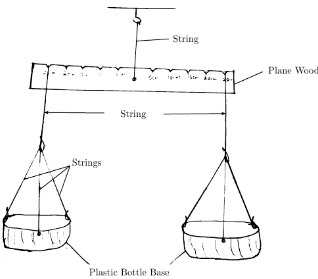
\includegraphics{./img/beam-balance.png}
\caption{A beam balance}
\label{fig:beam-balance}
\end{center}
\end{figure}

\subsubsection*{Activity Procedure}
Use the beam balance to measure the masses of different objects in the classroom.

\subsubsection*{Clean Up Procedure}
Return all materials to their proper places.

\subsubsection*{Discussion Question}
How can you improve the beam balance?

\subsubsection*{Notes}
There are different kinds of balances, such as a digital balance, double beam balance, single beam balance and triple beam balance. Each can be used to measure mass according to its sensitivity.

\subsection{Making a Spring and a Spring Balance}

\subsubsection*{Learning Objectives}
\begin{itemize}
\item{To make springs for various uses.}
\item{To create and calibrate a spring balance.}
\end{itemize}

\subsubsection*{Background Information}
Springs typically have a constant value which determines how much they can stretch or compress.  Because the value is constant, we can use it to accurately measure mass or weight, as it will always extend to the same length with the same force.

\subsubsection*{Materials}
Strong metal wire of swg 24 or 26 of various types like copper, nichrome or constantine; a rod of diameter 14 to 18 mm of any material, piece of wood, ruler, plane paper, known masses, glue.

\subsubsection*{Preparation Procedure}
Cut the metal wire into different lengths of at least 50 cm.

\subsubsection*{Activity Procedure}
\begin{enumerate}
\item{Take a piece of wire and hold one end to the rod.}
\item{Coil the wire tightly along the rod, keeping the coils close together.}
\item{When the entire wire is coiled along the rod, remove the rod.}
\item{Bend btoh ends of the wire into hooks.}
\item{Repeat these steps for all of the wires of different types and lengths.}
\item{Try stretching and compressing the springs to test the different strengths.}
\item{Attach the end of one spring to the top of a piece of wood with a nail or screw.}
\item{Glue or tape some white paper to the wood behind the spring.}
\item{Use a pen to make a mark at the bottom of the spring.}
\item{Hang a known mass on the spring so that it is stretched downward a short distance.}
\item{Make a mark at the bottom of the spring in its new position.  Label this with the mass of the object hung from the spring.}
\item{Repeat this process for other masses, marking each mass on the paper.}
\item{Use a ruler to finish the scale by filling in masses above, below and between the marks you have made.}
\end{enumerate}

\begin{figure}
\begin{center}
\def\svgwidth{150pt}
\input{./img/spring-balance.pdf_tex}
\caption{A Spring Balance}
\label{fig:spring-balance}
\end{center}
\end{figure}

\subsubsection*{Results and Conclusions}
When a load is placed on the spring, it increases the length of the spring.  When the load is removed, the spring returns to its original length.
Different materials of the same swg have different spring constants (strengths), or force per extension length.

\subsubsection*{Clean Up Procedure}
Return all materials to their proper places.

\subsubsection*{Discussion Questions}
\begin{enumerate}
\item{What are some uses of springs?}
\item{What are the qualities of a good spring?}
\item{What is the relationship between the wire's diameter and the strength of the spring?}
\item{Which metal makes the strongest spring?  Which metal makes the weakest spring?}
\end{enumerate}

\subsubsection*{Notes}
A good spring must obey Hooke's Law.  Springs can be used to make a spring balance or can be used in physics practicals to find the relationship between force and the resulting extension.

%Weight vs. Mass


%Density, Relative Density
	%See Density in Chem for more

\subsection{Applications of Material Densities}

\subsubsection*{Learning Objectives}
\begin{itemize}
\item{To observe the difference between densities of different liquids and solids.} 
\item{To design a density tower using a variety of liquids with different densities.} 
\end{itemize}

\subsubsection*{Background Information}
Materials can usually be distinguished from each other by their densities.  Normally, less dense materials float on denser liquids.  When liquids are placed in a container, the heavier (denser) liquids sink while the lighter (less dense) liquids float.  A density tower can be designed using liquids of different densities, even if they are soluble.

\subsubsection*{Materials}
Water, honey, glycerine, cooking oil, spirit, kerosene, beakers*, test tubes*, syringes, small pieces of wood, small pieces of rubber, small pieces of metal, and different food colour (optional).

\subsubsection*{Preparation Procedure}
\begin{enumerate}
\item{Find a test tube or syringe.}
\item{Place each liquid into a beaker so it can easily be obtained by students.} 
\end{enumerate}

\subsubsection*{Activity Procedure}
\begin{enumerate}
\item{Place a small amount of honey into the test tube.} 
\item{Slowly add glycerine to the test tube.} 
\item{Slowly pour water into the test tube.} 
\item{Slowly add methylated spirit to the test tube.} 
\item{Add cooking oil into the test tube.} 
\item{Slowly add kerosene to the test tube.} 
\item{Put a small piece of wood, rubber and iron into the test tube.}
\item{Observe the positions of the liquids and solids relative to each other.}

\end{enumerate}
\begin{figure}[h]
\begin{center}
\def\svgwidth{200pt}
\input{./img/density-tower.pdf_tex}
\caption{Density tower}
\label{fig:density-tower}
\end{center}
\end{figure}

\subsubsection*{Results and Conclusions}
The liquids with a higher density will sink, while the liquids with lower density will float. When the solid materials are dropped into the test tube, the solid material will rest in the liquid that has a relatively equal density.  

\subsubsection*{Clean Up Procedure}
Collect all materials and return them to their proper place.

\subsubsection*{Discussion Questions}
\begin{enumerate}
\item{Why should liquid be poured slowly into the test tube?}
\item{What happens when the wood, iron, and rubber are placed into test tubes?} 
\end{enumerate}

\subsubsection*{Notes}
Heavier density liquid should be poured into the test tube first, followed by relatively less dense liquids. Pouring the liquids should be done slowly to avoid mixing of liquid. Food colour can also be added to colorless liquid such as water, kerosene, and glycerine.  

\subsection{Relative Density of a Liquid}

\subsubsection*{Learning Objectives}
\begin{itemize}
\item{To determine the density and relative density of a liquid.} 
\end{itemize}

\subsubsection*{Background Information}
Bodies of different materials have different densities.  Density can be found by taking the ratio of a body's mass to its volume.  $$\mathrm{Density} = \frac{\mathrm{mass}}{\mathrm{volume}}$$

Relative density (R.D.) can be used to compare the density of a given material to that of water.  Water is the standard with a density of 1.0 g/mL, so all other densities are compared to water.
$$\mathrm{R.D.} = \frac{\mathrm{Density\; \; of \;substance}}{\mathrm{Density\; \;of \;water}}$$

\subsubsection*{Materials}
``Density bottle" (small empty can or bottle), rubber stopper/dry grass/maize cob*, plastic bag, water, honey, kerosene, cooking oil, straw/bamboo stick


\subsubsection*{Activity Procedure}
\begin{enumerate}
\item{Weigh the can with its stopper and plastic bag in air (variable \ce{M0}).} 
\item{Fill the small can with water and weigh it (variable \ce{M1}).} 
\item{Pour out the water from the can and dry it with a piece of clean cloth or tissue.} 
\item{Fill the can with another liquid, like honey, kerosene, or cooking oil, and weigh it again. (Variable \ce{M2})}
\item{Repeat steps 3 and 4 for other liquids}
\item Calculate the relative density of each liquid tested
\end{enumerate}

\subsubsection*{Results and Conclusions}
Mass of density bottle = \ce{M0}\\
Mass of density bottle with water = \ce{M1}\\
Mass of the density bottle with liquid A = \ce{M2}\\
$$\mathrm{Relative \;density \;of \;liquid \;}A = \frac{\mathrm{Mass \;of \;liquid \;}A}{\mathrm{Mass \;of \;water}} = \frac{M_2-M_0}{M_1-M_0}$$
We use this formula to find the relative density of any liquid.

\subsubsection*{Clean Up Procedure}
Collect all the used materials, cleaning and storing items that will be used later.

\subsubsection*{Discussion Questions}
\begin{enumerate}
\item{Determine the mass of the water.} 
\item{Calculate the volume of the density bottle and the relative density of honey.} 
\end{enumerate}

\subsubsection*{Notes}
A density bottle can also be used to find the density of a solid, liquid and granules.
When finding relative density, units must be considered carefully.  Before you find the ratio of liquid density to water density, be sure that the units are the same.  g/mL or kg/L are the common units.

\subsection{U-Tube apparatus}
\begin{itemize}
\item{Preparation Time: 1 hour}
\item{Materials: 3 clear plastic pen tubes, cardboard, hot poker or knife, tape, pen, super glue, water, any fluid, which will not readily mix with water.}
\item{Construction: Cut two of the pens at one end at a 45-degree angle, and cut the third pen (shorter than the other two) at both ends at a 45-degree angle. With the shorter pen on the bottom, attach the other two as styles so that the 45-degree angles meet to form right angles. Together the 3 pens should form a U-shaped tube with open ends at the top of each style (vertical tube). Melt the angled ends together with a hot knife, soldering iron, etc. so that the whole apparatus is watertight except for the tops. Glue the apparatus to a cardboard base so that it can stand up straight. Put thin strips of tape up each side of the U-tube and mark each strip with evenly spaced marks. The two scales should be identical. One good way to do this is to put steadily increasing volumes of water (3 ml, 4 ml, 5 ml, etc.) and mark the levels on each scale for each volume. Label these marks from top to bottom as 0, 1, 2, etc.}
\item{Procedure: Place an amount of water into the U-tube such that the water rises about half way on either side of the tube. The actual volume of water is not important as long as you can see the levels clearly. Stand the tube upright and slowly drip about 1 ml of another fluid, kerosene in this case, into one side of the U-tube (if the fluid has a higher density than water, it should go in first, and then the water). The kerosene will displace the water, so you should see the water level on the other side rise slightly.\\
Measure the relative heights of water and the kerosene from the bottom level of the kerosene. The heights are related to the densities by:
\[ \frac{\mathrm{Height of water}}{\mathrm{height of kerosene}} = \frac{\mathrm{density of kerosene}}{\mathrm{density of water}} \]
} % Procedure
\item{Theory: If a fluid’s density is less than that of water, it will float on top (if it is added slowly) of the water, displacing the water on the other side of the tube. From Archimedes’ principle and the Law of Flotation, we know that the relative density of the fluid is equal to the inverse ratio of the heights of the liquid. The scales drawn on the outside of the U-tube allow you to find the ratio of the heights without needing units, and the density of water is known to be 1.0 g/ml, so you can easily calculate the density of the other fluid.\\
If the other fluid has a higher density than water, the experiment can still be done, but you need to add the fluid with higher density first, then displace it with water, performing the same calculation.\\
This apparatus was designed and brought forward by two form 4 students without any prompting. They then proceeded to find the density of kerosene accurate to two decimal places. Never underestimate the curiosity and ability of students, or the power of broken pens.}
\end{itemize}

%Error in Measurement

\subsection{Measurement Errors}

\subsubsection*{Learning Objectives}
\begin{itemize}
\item{To understand the meaning of experimental error}
\item{To understand the importance of accurate measurement and sample size}
\end{itemize}

\subsubsection*{Background Information}
Measurement is one of the most important aspects of science. However, it is impossible to make a perfect measurement because of our own errors and errors in the tools that we use. To improve our accuracy, we take many measurements and compare them to get an average result. However, it is important to understand the source of errors, how to account for them and how to reduce them. Different people measure differently, and even one person will measure differently from one moment to another.

\subsubsection*{Materials}
Metre rules, stopwatches, other measuring instruments, materials to measure

\subsubsection*{Preparation Procedure}
Collect different tools used for measuring, like metre rules or rulers, stopwatches, syringes, etc.

\subsubsection*{Activity Procedure}
\begin{enumerate}
\item{Draw a line on the board or floor.}
\item{Have several students measure the line and secretly record their results.}
\item{Collect the results from the students and record them on the board. Observe any differences.}
\item{Distribute stopwatches to several students.}
\item{Clap twice; the students should measure the time between claps and record their results secretly.}
\item{Collect the results from the students and record them on the board. Observe any differences.}
\item{Have several students make other similar measurements, keeping their results secret until you record them on the board.}
\item{Have students decide what the best result is for each of the collected measurements.}
\end{enumerate}

\subsubsection*{Results and Conclusions}
The measurements will be different from person to person. Lengths, times, volumes, etc. will all vary for the same quantity. This is because each person measures slightly differently; this is fine as long as each person is trying their best to be accurate. The best result is the average of the results, combining the accuracy of all people in the final result.

\subsubsection*{Discussion Questions}
\begin{enumerate}
\item{Why do the measurements differ from student to student?}
\item{How accurate are the tools that we use?}
\end{enumerate}

\subsubsection*{Notes}
Be sure that students understand that error is not bad. Many science students feel that they need to make their answers better, even if it means changing their data. Every measurement ever made has an error. Some tools are better at measuring than others; we simply use what we have and measure as accurately as we can. However, error needs to be understood and taken into account when doing experiments.



%Shika



%\subsection{Measurement Errors}
%\begin{itemize}
%\item{Preparation time: 1 minute}
%\item{Materials: Meter sticks or stopwatches}
%\item{Procedure: Ask for several students to volunteer to help. If using stopwatches, tell them to measure the time between two claps that you will give. Clap once, at which time the students should start their stopwatches. After a period of several seconds, clap a second time, at which point the students should stop their stopwatches. Make a simple table of their results, including several intervals. Each student should have a slightly different measurement. As they were all measuring the same event, this shows that their measurements contain errors.\\
%Alternately, place a chalk mark on the wall at a height of more than 1 meter above the floor. Give several students a meter stick, and ask them to measure the height of the mark. Again, their answers should all be slightly different, because measurements always contain an error.\\
%For this demonstration, it may sometimes happen that the first student will report a certain value, and then all of the following students will agree with the first value, regardless of what they have measured. The students should not all get the same value. To prevent this false agreement, it may be necessary to have each student first write their measurement on a small piece of paper, and then hand all of the papers to you.}
%\end{itemize}
%
%\subsection{Beam balance}
%\begin{itemize}
%\item{Preparation Time: half hour}
%\item{Materials: Coat hanger, retort stand or other support, cardboard, pen, two water bottle bottoms, string, tape}
%\item{Procedure: Hang the coat hanger from the retort stand or support so that it is free to swing. Cut out a strip of cardboard with a single centerline and tape it to the stand upright. Cut out a cardboard pointer and tape it to the coat hanger so that when the hanger hangs level, the pointer lines up exactly with the centerline on the cardboard strip. Any swinging of the hanger should cause the pointer to drift from the line. Now hang the water bottle bottoms with string from each corner of the hanger (you can bend the hanger a bit so that the string does not slide in; the bottles act as scale pans. Make sure that the hanger still hangs level when nothing is placed in either scale pan; calibrate with extra bending or mass as necessary. With a little bit of fidgeting, you should have a decent beam balance ready for use!}
%\item{Theory: Beam balances do not need to be calibrated to specific masses; as long as they indicate clearly when two masses are equal, it is enough. If you have a set of known, graduated masses, you can do specific measurements.}
%\end{itemize}
%
%\subsection{Spring balance}
%\begin{itemize}
%\item{Preparation time: 1 hour}
%\item{Materials: pen springs, paper, ruler, known masses, pen, eye-hooks, glue}
%\item{Construction: Hang the spring(s) from an eye-hook in whatever frame you choose. From the bottom of the springs, hang the other eye-hook such that any weight can be hung again from it. On the bottom eye-hook place a pointer (paper, needle, etc.) facing sideways, then glue the paper over the frame so that the springs are free to move up and down and the pointer always points to some point on the paper (toothpaste boxes, glycerin boxes, etc. work well). Mark the pointer’s position when the springs hang freely, then when they hold 1 gram, 2 grams, etc.\\
%You now have a spring balance, though you will have to do your own work to make it smooth and structural depending on your materials. You can measure mass, acceleration due to gravity, and the spring constant. Every spring has a constant.}
%\end{itemize}
%\section{Forces}

% Concept of Force

\subsection{Making a Spring Balance} % Move to Force, Chapter 4

\begin{center}
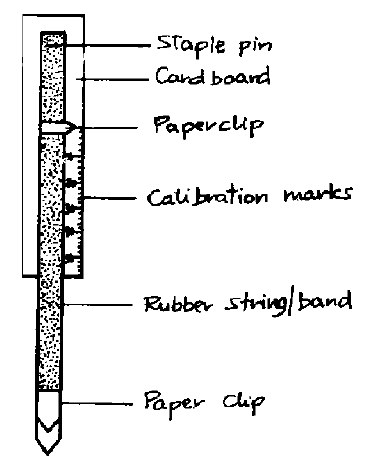
\includegraphics[width=6cm]{./img/source/spring-balance.png}
\end{center}

\begin{description*}
%\item[Subtopic:]{Concept of Force}
%\item[Shika Rating:]{4}
\item[Materials:]{Cardboard, strong rubber band, staple pin, 2 paper clips, \nameref{sec:masses}*}
\item[Setup:]{Take a strip of cardboard or wood and fix a strong rubber band to it using a staple pin. (The stronger the rubber band, the larger the force you can measure.) Attach one paper clip as a pointer as shown in the figure. Then fix another as a hook at the bottom end of the rubber band.}
\item[Procedure:]{Calibrate the balance in \emph{Newtons} using either a standard set of \nameref{sec:masses} or another spring balance. A mass of 10 g has a weight of 0.1 N; a mass of 100 g has a weight of 1 N, etc. Draw marks accordingly on the scale of the balance.}
\item[Hazards:]{Never apply such a large force that the pointer does not return to the zero mark when the force ceases.}
%\item[Questions:]{}
%\item[Theory:]{}
%\item[Applications:]{}
%\item[Notes:]{}
\end{description*}


%Gravitational Force and Weight

\subsection{Presence of Gravity}

\subsubsection*{Learning Objectives}
\begin{itemize}
\item{To identify the force of gravity as it acts on falling bodies} 
\item{To identify the effect of air resistance on falling bodies} 
\end{itemize}

\subsubsection*{Background Information}
All objects on the earth experience a force of attraction exerted by the earth.  This is a natural force called Gravity and it acts on all bodies at all times.  The force of gravity varies from one point to another; some areas experience stronger gravity than others, but this effect is not noticeable.  All objects are pulled by gravity with equal force, regardless of their weights or masses.

\subsubsection*{Materials}
Various objects, a piece of paper, and a book (the book should be the same size or bigger than the paper)

\subsubsection*{Activity Procedure}
\begin{enumerate}
\item{Hold the various objects at shoulder height.} 
\item{Drop the objects to the ground one at a time. Repeat this step, but releasing the objects at the same time.} 
\item{Observe if there is any difference in speed as the objects fall to the ground.} 
\item{Hold a piece of paper at shoulder height and then release it.} 
\item{Place a piece of paper on top of a book and hold the book flat at shoulder height.} 
\item{Release the two items together and observe any differences between the motion of the paper by itself and of the paper and book together.} 
\item{Bunch the paper into a tight ball and drop it again.}
\end{enumerate}

\subsubsection*{Results and Conclusions}
It will be seen that all objects, with the exception of paper and other light, wide objects, fall at exactly the same rate. This is because the acceleration due to gravity for all objects on earth is the same.  
The paper, however, falls very slowly. This is not because gravity pulls less on paper; it is because the paper is more affected by air resistance. All objects are affected by air resistance, but it is most obvious with objects that have a small weight but a large surface area. The effects of air resistance can be greatly reduced by placing a book under the paper. The book moves easily through air and blocks all of the air which would normally push against the paper. This is why the paper and book fall at the same rate.  When the paper is bunched into a ball, the mass stays the same but the air resistance is greatly reduced so it should fall at the same rate as the book.

\subsubsection*{Clean Up Procedure}
Collect all materials and return them to their proper place.

\subsubsection*{Discussion Questions}
\begin{enumerate}
\item{Did the objects fall at the same rate or at different rates?}
\item{Why did the paper fall slowly the first time?}
\item{Why did the paper fall quickly when it was placed on top of the book?}
\item{Why did the paper fall quickly when it was bunched into a tight ball?}
\item{What force is pulling all objects down? Does this force ever change?}
\end{enumerate}

\subsubsection*{Notes}
When performing this experiment, it is important to remember the effect of air resistance.  Gravity pulls equally on all bodies, but air resistance opposes the motion of light-weight objects more effectively than heavy-weight objects.

%Types / Effects of Forces


%Air Resistance

\subsection{Windmills}
\begin{itemize}
\item{Preparation Time: 15 minutes}
\item{Materials: thin cardboard or cardstock, scissors, pen, colored pencils/markers if desired, glue, paper fastener or thumb tack, straw or stick}
\item{Procedure: Use the following illustration (enlarge it); copy it onto a piece of thin cardboard or cardstock.}
\begin{enumerate}
\item{Cut along the lines and make holes with a pencil or pen.}
\item{Bend the four corners together into the center and glue them in place.}
\item{Push the fastener or tack through the center hole into a straw or stick.}
\end{enumerate}
\item{Reference: This demo was published in the Science Lab Kit by Silver Dolphin Books in 1997, compiled by Brenda Walpole}
\end{itemize}

\subsection{Helicopters}
\begin{itemize}
\item{Preparation Time: 15 minutes}
\item{Materials: paper, scissors, paper clip}
\item{Procedure: Copy the following design onto a piece of paper. Cut along the solid lines and fold along the dotted lines, attaching the paper clip to the bottom. Drop the helicopter with the paperclip down and watch it spin!
*This demo was published in the Science Lab Kit by Silver Dolphin Books in 1997, compiled by Brenda Walpole}
\end{itemize}

\begin{figure}[h!]
\begin{center}
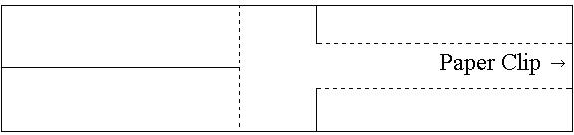
\includegraphics[width=0.45\textwidth]{./img/helicopter-1.png}
\caption{Paper helicopter template}
\label{fig:helicopter-1}
\end{center}
\end{figure}

\begin{figure}[h!]
\begin{center}
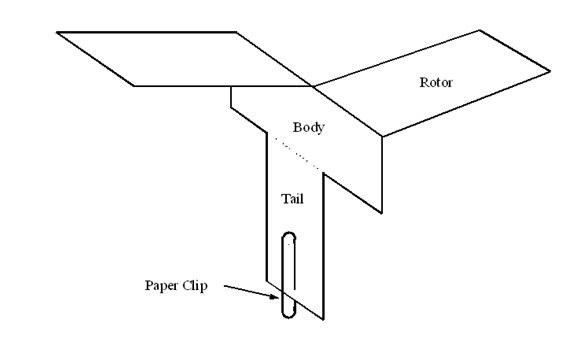
\includegraphics[width=0.6\textwidth]{./img/helicopter-2.png}
\caption{Paper helicopter construction}
\label{fig:helicopter-2}
\end{center}
\end{figure}
%\section{Archimedes' Principle and the Law of Flotation}


%Eureka Can


\subsection{Construction of Eureka Can}

\subsubsection*{Learning Objectives}
\begin{itemize}
\item{To construct a eureka can and use it to measure volumes of irregular objects.} 
\end{itemize}

\subsubsection*{Materials}
Plastic bottles of 500 mL or 1000 mL, straws* or a syringe needle cap, a knife/razor blade, heat source*, cellotape or super glue, nail, and a wire

\subsubsection*{Preparation Procedure}
\begin{enumerate}
\item{Cut the plastic bottle in half and use the bottom part.} 
\item{Heat a sharp pointed end of the nail.} 
\item{Using the heated sharp point of the nail, make a small hole about 5 cm from the top of the cut plastic bottle.} 
\item{Cut a piece of straw about 5 cm long or use the syringe needle cap.} 
\item{Insert the piece of straw into the hole. Make sure the piece of straw is tightly fixed with cellotape or super glue.} 
\end{enumerate}

\subsubsection*{Activity Procedure}
Use the constructed eureka can to overflow different liquids and to measure the volume of liquid displaced when an object floats in it.

\subsubsection*{Clean Up Procedure}
Collect all the used materials, cleaning and storing items that will be used later.

\subsubsection*{Discussion Questions}
\begin{enumerate}
\item{What is the relationship between the weight of a floating object and the weight of water it displaces?}
\item{What is the reason for using a Eureka Can instead of a normal bottle?}
\end{enumerate}

\subsubsection*{Notes}
A Eureka Can is typically used to move a certain volume from the can into another container.  When an object floats in a liquid, it displaces its own weight in water.  If the level of water in the Eureka can is at the level of the spout, the water displaced will flow through the spout into another container.  This water can then be measured on a beam balance to find the weight of the object.



\subsection{Water Weight and Upthrust}
\begin{itemize}
\item{Preparation Time: 1 minute}
\item{Materials: spring balance, syringe with the bottom melted shut and no plunger, eureka can (can be made cheaply by a metal craftsman), water, heavy object, thread, small dish}
\item{Procedure: Fill the eureka can up to its spout with water and place the spout over the dish. This can is designed so that when the water is being displaced, it is collected to another container for later measurements. Hang the object by the thread from the spring balance and measure its weight. Now immerse the water completely in the eureka can and measure its Apparent Weight (weight in water).\\
When you immersed the object in water, some water will have overflowed from the can into the small dish. Pour this water into your syringe shell and measure the weight of water. Record this result with the earlier Weight and Apparent Weight.}
\item{Theory: Archimedes’ Principle states that the upthrust of a liquid on an object is equal to the weight of water displaced by the object. The upthrust is equal to the Weight of the object minus its Apparent Weight in the water:@	Upthrust = Weight in air – Apparent Weight in liquid\\
But upthrust is also equal to the water displaced:@	Upthrust = Weight of liquid displaced\\
By calculating the upthrust, you should see that the result is equal to the weight of water in the syringe.}
\end{itemize}


%Sinking and Floatinng


%\subsection{Floating Eggs}
%\begin{itemize}
%\item{Preparation time: 5 minutes}
%\item{Materials: 1 uncooked egg, 1 jam jar, water, salt}
%\item{Procedure: Fill jam jar with water. Place egg in the water. The egg will sink. Add salt until the egg floats.}
%\item{Theory: The density of an egg is greater than water. This is why the egg will sink. Since density is defined as mass divided by volume, the density of water can be changed by dissolving extra mass, salt in this case. As more and more salt dissolves in the water, the densities increases until the density of the water is greater than the egg and the egg floats to the surface.\\
%This is the same reason why it is more difficult to swim in fresh water than salt or ocean water. The extra salt or ions in the ocean water increase its density and making the body more buoyant. Since those ions are much fewer in fresh water, the density of fresh water is greater than salt water. The Dead Sea in the Middle East has so much salt in the water that people do not swim in the water; they just float. Lake Natron in Tanzania probably has similar properties.}
%\end{itemize}



\subsection{Conditions of Flotation}

\subsubsection*{Learning Objectives}
\begin{itemize}
\item{To explain the conditions for a floating body.} 
\end{itemize}

\subsubsection*{Materials}
Water, fresh egg, salt, beaker*

\subsubsection*{Activity Procedure}
\begin{enumerate}
\item{Fill a beaker with water.} 
\item{Release a fresh egg on the surface of water slowly and observe its position.} 
\item{Add some salt while stirring and observe the position of the egg.} 
\item{Continue adding salt and observe the position of the egg.} 
\end{enumerate}

\subsubsection*{Results and Conclusion}
The egg sinks to the bottom of the container because its density is greater than that of water. After adding the salt, the egg rises and finally floats on the surface of water. This is because the density of the water becomes higher than that of the egg.  

\subsubsection*{Clean Up Procedure}
Collect all the used materials, cleaning and storing items that will be used later.

\subsubsection*{Discussion Questions}
\begin{enumerate}
\item{Why does the egg sink initially?}
\item{What causes the egg to float after the addition of salt?}
\end{enumerate}

\subsubsection*{Notes}
An object immersed in water experiences upward force equal to the weight of the water it displaces. The upthrust competes with the downward pull of gravity which diminishes the weight of the object. If the upthrust is greater than the object's weight, it will float. Otherwise, the object will sink. If the water density is greater than the average density of the object, the object will also float. If the water density is less than the average density of the object, the object will sink.  


%Law of Flotation


%Hydrometer


\subsection{Construction and Use of a Hydrometer}

\subsubsection*{Learning Objectives}
\begin{itemize}
\item{To construct a simple hydrometer.} 
\item{To explain the use of a hydrometer.} 
\item{To calibrate a hydrometer.} 
\item{To use a hydrometer to measure the density of various liquids.} 
\end{itemize}

 \begin{figure}
\begin{center}
\def\svgwidth{150pt}
\input{./img/hydrometer.pdf_tex}
\caption{A Hydrometer}
\label{fig:hydrometer}
\end{center}
\end{figure}

\subsubsection*{Background Information}
Each liquid has a different density. The level at which an object will float in a liquid depends on the density of that liquid, so the different densities of liquids can be observed and measured by observing the level at which an object floats in them.  

\subsubsection*{Materials}
Plastic straw, small piece of plastic bag, dry sand, several containers to hold liquids, marker pen, rubber band or thread, ruler, water, kerosene, honey, any other liquids

\subsubsection*{Preparation Procedure}
\begin{enumerate}
\item{Close one end of the straw with the plastic bag and secure it with the rubber band or thread so that water cannot enter.} 
\item{Place the straw in water with the plastic bag side down.} 
\item{Pour sand into the straw until the bottom is heavy enough that the straw floats upright.} 
\end{enumerate}

\subsubsection*{Activity Procedure}
\begin{enumerate}
\item{Place the straw in water so that it floats upright without touching the bottom or leaning.} 
\item{Use the marker pen to mark the water level on the outside of the straw. Label this mark as 1.0 (the known density of water).} 
\item{Place the straw in a container of kerosene so that it floats upright without touching the bottom or leaning to one side.} 
\item{Use the marker to mark the kerosene level on the outside of the straw. Label this mark as 0.8 (the known density of kerosene).}
\item{Remove the straw from the kerosene and clean it. Be careful not to get any liquid inside the straw.} 
\item{Use a ruler to draw an accurate scale on the straw, using the 1.0 and 0.8 marks as starting points. Begin by making a mark directly between them as 0.9, etc.} 
\item{When the scale is complete (both above 1.0 and below 0.8), use the designed hydrometer to measure the densities of other liquids by reading the mark at the level of the liquid.} 
\end{enumerate}

\subsubsection*{Results and Conclusions}
The straw, when properly weighted, will float upright in any liquid and will therefore provide a good surface to write levels of liquids. The density of water is known as 1.0 and is relatively constant. Kerosene is also known as 0.8 and will not vary from place to place. By writing both of these points on the hydrometer and the respective floating levels, we can create a scale extending up from 1.0 and down from 0.8. This can then be used to measure the densities of other liquids.  

\subsubsection*{Clean Up Procedure}
\begin{enumerate}
\item{Return all liquids to their proper containers.} 
\item{Clean the outside of the hydrometer.} 
\item{Return all materials to their proper places.} 
\end{enumerate}

\subsubsection*{Discussion Questions}
\begin{enumerate}
\item{What liquids have high density?}
\item{What liquids have low density?}
\item{Why, when reading a hydrometer, do the small numbers appear at the top of the scale?}
\end{enumerate}

\subsubsection*{Notes}
Be careful not to get any liquid in the straw. If the sand becomes wet, the hydrometer will not work again until it dries.  
%\section{Structure and Properties of Matter}

%States of Matter


%Particles / Kinetic Theory of Matter


%Elasticity


%Adhesion and Cohesion


\subsection{Determining Adhesion and Cohesion}

\subsubsection*{Learning Objectives}
\begin{itemize}
\item{To observe cohesion and adhesion forces of different liquids.}
\item{To determine adhesive forces between water molecules.}
\item{To determine cohesive forces between different liquids.}
\end{itemize}

\subsubsection*{Background Information}
Adhesion is the force of attraction between a material and its surroundings. Cohesion is the force of the liquid molecules to stick to themselves. The concept of adhesive and cohesive forces can be used in different ways such as determination of viscosity of the liquids and explaining the transportation of liquid in plants and animals. When a drop of water is placed on a sheet of glass, the water spreads because adhesive forces between glass and water are greater than the cohesive forces between water molecules. When a drop of honey, cooking oil, or glycerine is placed on a sheet of glass, it remains almost spherical because the cohesive force is greater than the adhesive force.

\subsubsection*{Materials}
Sheet of glass, water, honey, glycerine, cooking oil, syringe, and 2 wooden blocks

\subsubsection*{Activity Procedure}
\begin{enumerate}
\item{Place 2 wooden blocks on the top of the table.}
\item{Place a piece of pane glass horizontally over the two wooden blocks.}
\item{Using a syringe, place different drop of liquids on top glass. Record your observations.}
\end{enumerate}

\begin{figure}[h]
\begin{center}
\def\svgwidth{200pt}
\input{./img/adhesion-cohesion.pdf_tex}
\caption{Observing adhesive and cohesive forces}
\label{fig:adhesion-cohesion}
\end{center}
\end{figure}

\subsubsection*{Results and Conclusions}
When a drop of water is placed on top of glass, water spreads and wets the glass. While material like honey, glycerine, and cooking oil remain in a spherical shape. The adhesive forces between the water molecule and glass molecule is greater. While the cohesive forces between the molecule of honey, glycerine and cooking oil is larger.

\subsubsection*{Clean Up Procedure}
Collect all the used materials, cleaning and storing items that will be used later.

\subsubsection*{Discussion Questions}
\begin{enumerate}
\item{Explain why water wets the glass while glycerine does not wet the glass.}
\item{Discuss where we apply the concept of adhesive and cohesive forces in other areas of science.}
\item{How are cohesion and viscosity related?}
\end{enumerate}

\subsubsection*{Notes}
The liquids which have the greatest forces of cohesion are also those with the highest viscosity.


%\subsection{Pinching Water}
%\begin{itemize}
%\item{Preparation Time: 10 minutes}
%\item{Materials: 0.5 liter bottle, water, pin or small nail}
%\item{Procedure: At the bottom of the side of the can or bottle, poke five small holes close together with the syringe needle or nail. Be careful not to let the holes overlap or be too far apart. Pour water into the bottle and allow the water to start flowing out of the holes at the bottom. Using your thumb and forefinger, pinch the streams of water together so that they form a single stream (this takes some practice). To undo your great work of creation, pass your hand in front of the holes and five streams will appear again.}
%\item{Theory: Water has a tendency to “cling” to itself due to its surface tension and cohesion. As you bring the streams together, you allow the water to stick to itself forming a single stream. Passing your hand in front again stops the flow of water at the holes and allows it to start again, which it will do in five streams.}
%\end{itemize}


\subsection{Cohesion in a Moving Liquid}

\subsubsection*{Learning Objectives}
\begin{itemize}
\item{To observe the effect of cohesion on moving water}
\end{itemize}

\subsubsection*{Background Information}
Cohesion is the force between molecules in a liquid. It holds liquids like water together if they are standing still or moving.

\subsubsection*{Materials}
Empty 0.5 litre bottle, water, syringe needle OR pin OR small nail

\subsubsection*{Preparation Procedure}
Make five small holes at the bottom of the side of the bottle. Make the holes close together (about 5 mm apart) with the syringe needle or nail.

\subsubsection*{Activity Procedure}
\begin{enumerate}
\item{Pour water into the bottle and allow the water to start flowing out of the holes at the bottom.}
\item{Using your thumb and forefinger, pinch the streams of water together so that they form a single stream.}
\item{To separate the streams again, pass your hand in front of the holes and the five streams will appear again.}
\end{enumerate}

\subsubsection*{Results and Conclusions}
When you pinch the streams of water together, they form a single stream or a few streams. Water has a tendency to cling to itself due to its surface tension and cohesion. As you bring the streams together, you allow the water to stick to itself forming a single stream. Passing your hand in front again stops the flow of water at the holes and allows it to start again, which it will do in five streams.

\subsubsection*{Clean Up Procedure}
Return all materials to their proper places.

\subsubsection*{Discussion Questions}
\begin{itemize}
\item{How did the behaviour of the water streams change as the level in the bottle decreased?}
\item{What force holds the water streams together?}
\item{Why do the streams eventually split?}
\end{itemize}

\subsubsection*{Notes}
Be careful not to let the holes overlap or be too far apart. This will cause the water to form one stream from the beginning or make it impossible to pinch the streams. Practice pinching the water and make new holes if necessary.


%Surface Tension


\subsection{Water drops}
\begin{itemize}
\item{Preparation time: none}
\item{Materials: Water dropper or syringe}
\item{Procedure: Slowly drip water from the water dropper or syringe and point out that before a drop falls; it will hang suspended by its surface tension. Explain that as the drop becomes larger, its weight increases until surface tension is insufficient to support it, at which point it falls.}
\end{itemize}

\subsection{Blowing bubbles}
\begin{itemize}
\item{Preparation time: 5 minutes}
\item{Materials: Thin piece of wire (approximately 30cm), water, detergent, glycerin (optional)}
\item{Procedure: Bend the wire into a loop 2 to 3 cm in diameter. Continue to bend the wire so that it circles around the circumference of this circle several times. Leave a straight piece several centimeters long to use as a handle. This is the “bubble blower”. Dip the circular part of the bubble blower into a strong solution of detergent (regular powdered laundry detergent works well) mixed with glycerin. When you remove the bubble blower from the solution, a thin film should remain across the circle. Gently blow through the center of the circle. With a little practice, you should be able to cause a spherical bubble to separate from the blower and float away.}
\item{Theory: The detergent causes the surface tension in the solution to be slightly variable. In areas of higher concentration of detergent, the surface tension is lower. In order for the films and bubbles to be stable, the surface tension near the top must be slightly higher than at the bottom. As the detergent molecules are heavier than water, they tend to sink towards the bottom of the film, accomplishing this.\\
When you blow through the bubble blower, we can see that then tension is pulling it back towards a flat surface. Once an independent bubble is formed, we see that it forms a nearly perfect sphere. This is because the surface is under tension. This tension forces the bubble to form the shape with the minimum surface area, a sphere. It is also worth noting that both the film that stays on the bubble blower and the bubbles themselves appear to have small rainbows of colors in them. This is caused by thin-film interference.}
\end{itemize}


%\subsection{Surface Tension in Bubbles}
%
%\subsubsection*{Learning Objectives}
%\begin{itemize}
%\item{To observe the effect of surface tension in soapy water}
%\end{itemize}
%
%\subsubsection*{Background}
%Surface tension is the force which holds the molecules together on the surface of a liquid. It can be strong enough that insects can walk on water, or objects with high density can float on a liquid. Bubbles form under the force of surface tension. As the surface of a liquid naturally forms a shape with the smallest surface area, a thin film of liquid will form a sphere, held together by surface tension around air. The air inside pushes out with equal force that air outside pushes in. Bubbles do not form easily in water, so a soapy solution is needed.
%
%\subsubsection*{Materials}
%Thin piece of wire (approximately 30cm), water, detergent, glycerin (optional)
%
%\subsubsection*{Preparation Procedure}
%\begin{enumerate}
%\item{Bend the wire to form a loop of 2 to 3 cm in diameter.}
%\item{Continue to bend the wire so that it circles around the circumference of this circle several times.}
%\item{Leave a straight piece several centimeters long to use as a handle. This is the bubble blower.}
%\item{prepare a concentrated solution of detergent by mixing powdered soap in water with a small amount of glycerin.}
%\end{enumerate}
%
%\subsubsection*{Activity Procedure}
%\begin{enumerate}
%\item{Dip the circular part of the bubble blower into the detergent.}
%\item{When you remove the bubble blower from the solution, a thin soapy film should remain across the circle.}
%\item{Gently blow through the center of the circle. With a little practice, you should be able to cause a spherical bubble to separate from the blower and float away.}
%\end{enumerate}
%
%\subsubsection*{Results and Conclusions}
%When you blow through the bubble blower, we can see that the tension is pulling it back towards the surface. Once an independent bubble is formed, we see that it forms a nearly perfect sphere. This is because the surface is under tension. This tension forces the bubble to form the shape with the minimum surface area, a sphere.
%
%\subsubsection*{Clean Up Procedure}
%Return all materials to their proper places.
%
%\subsubsection*{Discussion Questions}
%\begin{enumerate}
%\item{What is inside the bubble?}
%\item{Compare the pressure inside the bubble to the pressure outside the bubble.}
%\item{Why do bubbles form easily in soapy water but not in fresh water?}
%\end{enumerate}
%
%\subsubsection*{Notes}
%Try making the solution without glycerin and note any different results.\\
%It will be seen that the bubbles have colours; this is due to thin film interference, or the refraction of white light in a thin liquid medium.


\subsection{Pin Float}
\begin{itemize}
\item{Preparation time: none}
\item{Materials: A cup or small dish, a straight pin, water, detergent}
\item{Procedure: Make sure the cup or dish is clean, and has no soap or detergent residue. Fill the cup or dish with clean water. Carefully place the straight pin on the surface of the water, being careful not to break the surface. If done properly, it should be possible to get the straight pin to remain suspended on the surface (see also floating compass). Next, sprinkle a small amount of detergent onto the water. The pin should sink to the bottom.}
\item{Theory: When the straight pin is placed on the surface, it causes the surface of the water to bend downwards. This means that the surface tension of the water is pulling the pin upwards. Although the pin is denser than water, and would normally sink, this surface tension is enough to support the weight of the pin. When detergent is sprinkled onto the surface of the water, it lowers the surface tension of the water. The surface tension is no longer strong enough to hold up the pin, so the pin sinks.}
\end{itemize}

\subsection{Pepper Float}
\begin{itemize}
\item{Preparation time: none}
\item{Materials: A cup or dish, water, ground black pepper, soap or detergent}
\item{Procedure: Make sure that the cup or dish is clean, and has no soap or detergent residue. Fill the cup or dish with clean water. Sprinkle ground black pepper over the surface of the water in a way that the pepper is distributed evenly and covers the whole surface. Next, apply a small amount of soap or detergent to one finger. Touch this finger to the surface of the water in the center of the cup or dish. The pepper will flee your finger, and all run to the sides of the cup or dish.}
\item{Theory: When you touch your finger to the surface, you introduce a small amount of soap or detergent, lowering the surface tension at that point. The surface of the water is now unbalanced – the surface tension near the edge is pulling the surface outwards more strongly than the surface tension at the center is pulling the surface inwards. As there is a net force on the surface outwards towards the edge, the surface moves, pulling the pepper along with it to the edges of the cup or dish.}
\end{itemize}

%\subsection{Changing Surface Tension}
%
%\subsubsection*{Learning Objectives}
%\begin{itemize}
%\item{To observe the effect of surface tension}
%\item{To observe the effect of an impurity on the surface tension of water}
%\end{itemize}
%
%\subsubsection*{Background Information}
%Surface tension holds the molecules of a liquid together at the surface. However, the surface tension is not uniform; it depends on the composition of the liquid as well as the other forces present. In this experiment, we observe the effects of changing the surface tension.
%
%\subsubsection*{Materials}
%Cup or dish, water, ground black pepper, soap or detergent
%
%\subsubsection*{Preparation Procedure}
%Make sure that the cup or dish is clean, and has no soap or detergent residue.
%
%\subsubsection*{Activity Procedure}
%\begin{enumerate}
%\item{Fill the cup or dish with clean water.}
%\item{Sprinkle ground black pepper over the surface of the water in a way that the pepper is distributed evenly and covers the whole surface.}
%\item{Apply a small amount of soap or detergent to one finger.}
%\item{Using this finger, touch the surface of the water at the center of the cup or dish.}
%\end{enumerate}
%\subsubsection*{Results and Conclusions}
%When your finger touched the center of the surface of the water, the pepper moves quickly towards the edge of the water. This is because as your finger touches the surface, you introduce a small amount of soap or detergent, lowering the surface tension at that point. The surface of the water is now unbalanced; the surface tension near the edge is pulling the surface outwards more strongly than the surface tension at the center is pulling the surface inwards. As there is a net force on the surface outwards towards the edge, the surface moves, pulling the pepper along with it to the edges of the cup or dish.
%
%\subsubsection*{Clean Up Procedure}
%Dispose of the water and return all materials to their proper places.
%
%\subsubsection*{Discussion Questions}
%\begin{enumerate}
%\item{Why does the pepper move quickly away from the center?}
%\item{What happens if you add other liquids instead of soap?}
%\end{enumerate}
%
%\subsubsection*{Notes}
%Floating objects will tend towards the area with highest surface tension. The pepper in this case is following the higher surface tension towards the side of the container.


\subsection{Water Dome}
\begin{itemize}
\item{Materials: Coin, water, syringe or eyedropper}
\item{Preparation Time: none}
\item{Procedure: Place a coin flat on the table. Using the syringe or eyedropper, carefully drop individual water drops onto the coin. With some practice, you should be able to get quite a few drops onto the coin before the water spills over, creating a dome of water.}
\item{Theory: The surface tension of the water holds it together against the force of gravity, which is trying to pull the water off the coin.}
\end{itemize}


%\subsection*{Water Dome}
%
%\subsubsection*{Learning Objectives}
%\begin{itemize}
%\item{To observe the strength of surface tension and cohesion}
%\end{itemize}
%
%\subsubsection*{Background Information}
%Surface tension can be surprisingly strong. Insects and objects can float on top of water because of its tension; also water itself holds together in droplets. Combining droplets allows cohesion to form more bonds, creating a larger droplet with the same surface tension.
%
%\subsubsection*{Materials}
%Coin, water, syringe or eyedropper
%
%\subsubsection*{Activity Procedure}
%\begin{enumerate}
%\item{Place a coin on the table.}
%\item{Using the syringe or eyedropper, carefully drop individual water drops onto the coin. With some practice, you should be able to get quite a few drops onto the coin before the water spills over, creating a dome of water.}
%\end{enumerate}
%
%\subsubsection*{Results and Conclusions}
%As you add more water to the coin, the water forms a larger and larger dome rather than spilling off the coin. The surface tension of the water holds it together against the force of gravity, which is trying to pull the water off the coin. 
%
%\subsubsection*{Clean Up Procedure}
%Return all materials to their proper places.
%
%\subsubsection*{Discussion Questions}
%\begin{enumerate}
%\item{How many drops did you think would fit on the coin? How many actually did fit?}
%\item{Why does the water dome eventually break?}
%\item{Describe all the forces acting on the water.}
%\end{enumerate}
%
%\subsubsection*{Notes}
%The most dramatic results can be see on small coins, though big coins can also be used. You should be able to get at least 60 drops on a 200 shilling coin.


%Capillarity


\subsection{Capillarity}

\subsubsection*{Learning Objectives}
\begin{itemize}
\item{To observe the effect of capillarity in various liquids.} 
\item{To explain the mode of action of capillarity.} 
\end{itemize}

\subsubsection*{Background Information}
Capillarity, or capillary action, is possible because of the combined effects of cohesion and adhesion. Cohesion holds a liquid together, especially at the surface. Adhesion allows a liquid to attach itself to another material, like the vertical surface of a container. 

\subsubsection*{Materials}
Clear thin plastic straws with different diameters, shallow container (bottom of a water bottle, jar cap), various liquids like water, spirit, cooking oil, and kerosene 

\subsubsection*{Activity Procedure}
\begin{enumerate}
\item{Pour some water into the container so that it is about 1 cm deep.} 
\item{Place one end of the straw into the liquid so that the end is completely submerged but not touching the bottom of the container.} 
\item{Observe the change in water level in the straw for about a minute.} 
\item{Repeat these steps for the other liquids and compare.}
\item{Repeat these steps for straws of different diameters and compare.} 
\item{Repeat these steps for different liquids and compare.} 
\end{enumerate}

\subsubsection*{Results and Conclusions}
Liquid in a thin tube will slowly climb up the tube without any visible force present. Adhesion and cohesion are pulling the liquid up the tube. The capillary action of the liquid depends on the diameter of the tube. Different liquids have different capillary action for the same size capillary.

\subsubsection*{Clean Up Procedure}
\begin{enumerate}
\item{Return all liquids to their proper containers and put them away.} 
\item{Wash the container and straw and put them away.} 
\end{enumerate}

\subsubsection*{Discussion Questions}
\begin{enumerate}
\item{What causes the liquid to move up the straw?}
\item{What causes the liquid at the edge to cling to the straw while the liquid in the middle remains lower?}
\item{Which liquid moved up the straw fastest? Which moved slowest?}
\item{What would happen if the diameter of the straw was increased? What would happen if it was decreased?}
\end{enumerate}

\subsubsection*{Notes}
Liquids are able to climb up a thin tube due to the combined effects of adhesion and cohesion. Cohesion allows a liquid to remain connected to itself while adhesion allows a liquid to remain connected to another surface. Adhesion causes a liquid to climb slightly up the side of any container; the surface tension of the liquid (cohesion) then pulls the remainder of the liquid up as well. In a normal container, the adhesive force at the side of the container is not strong enough to pull all the other liquid up. In a thin container, a larger proportion of liquid is attached to the side of the tube and a smaller proportion is being held by surface tension, so the adhesive force is strong enough to pull all the liquid up the tube.



%Diffusion


\subsection{Lemonade}
\begin{itemize}
\item{Preparation Time: 5 minutes}
\item{Materials: lemon, drinking water, pitcher}
\item{Procedure: Make lemonade by putting lemon wedges (oranges also work) into the pitcher and adding about a liter of water. Let it sit for a couple hours, then drink and enjoy! Adding sugar or honey is recommended.}
\item{Theory: The citrus flavor of the lemons will gradually spread throughout the water, though no force is apparent. This process is called diffusion. See the Transport topic in the Biology section for more activities involving diffusion.}
\end{itemize}


\subsection{Powder Diffusion}
\begin{itemize}
\item{Preparation time: 0 minutes}
\item{Materials: powdered food coloring or kool-aid like product, water, plastic water bottle}
\item{Procedure: Fill the plastic water bottle with water. Quickly add the powdered food color, but do not shake. Observe the color diffuse through the water.}
\item{Theory: Mixing does not occur immediately. Without shaking or stirring, it occurs slowly. By using a colored compound, it is easy to see how the molecules are slowly dissolving into the solution.}
\end{itemize}

\subsection{Orange Diffusion, Part A -- Sweet Smells}
\begin{itemize}
\item{Preparation time: 5 minutes}
\item{Materials: one orange or other citrus fruit}
\item{Procedure: Have students sit in their seats. Start to peel the orange. When students begin to smell oranges, have them raise their hands. Be sure the students only raise their hands as they smell the orange and not before.}
\item{Theory: Diffusion happens in not only liquids but also gases. Peeling oranges or other citrus fruits releases small compounds that diffuse through gases. When these compounds come in contact with out noses, we smell oranges. However, we cannot smell oranges immediately on peeling; the compounds must migrate towards our noses. In this case, the compounds will slowly diffuse in the classroom with the students closest to the orange smelling it first. The students in the back of the classroom will smell it last. The effects of wind should be considered.}
\end{itemize}

\subsection{Orange Diffusion, Part B -- Trapped}
\begin{itemize}
\item{Preparation time: 5 minutes}
\item{Materials: a box, one orange or other citrus fruit}
\item{Procedure: Turn the box upside down. Without turning the box over, peel the orange inside of the box. When students begin smelling oranges, have them raise their hands.}
\item{Theory: Diffusion can only occur when the molecules can move freely. Some objects will not allow compounds through. In this activity, the cardboard box prevents the compounds in the orange to diffuse out through the classroom. This time, students not smell oranges or it will take a long time for students to start smelling.}
\end{itemize}


%Osmosis


\subsection{Osmosis}
\begin{itemize}
\item{Preparation time: 10 minutes}
\item{Materials: 1 potato or carrot, water, salt, two water bottle bottoms}
\item{Procedure: Cut two equal sized pieces of potato. Put one piece is normal water and the other in a salt-water solution. Observe over the next few hours.}
\item{Theory: In all cells and plants, there is a proper balance of different concentrations of salts and sugars. Osmosis is the process where the salts move from a high concentration either to a low concentration or where water moves from a low concentration to a high concentration. In this activity, placing the potato in pure water will cause the potato to swell. Inside the potato, there is a higher concentration of salts and sugars compared to the water surrounding it. The water moves into the potato in order to make the concentrations inside the potato more similar to the water. The potato swelling is visual evidence of this phenomenon. The potato in salt water has exactly the opposite effect. The concentration of salts inside the potato is much lower compared to the concentration of salt in the water surrounding the potato. The water in the potato moves out of the potato to dilute the salt solution.}
\end{itemize}
%\section{Pressure}

%Concept of Pressure

\subsection{Balloon Pop}
\begin{itemize}
\item{Preparation Time: 20 minutes}
\item{Materials: piece of wood, nails, water balloons, water}
\item{Procedure: Put one nail through the board in one place and a large cluster of closely spaced nails in another place, all pointing up. Fill a balloon with water. As you lower the balloon onto the single or few nails, the balloon eventually pops. Fill another balloon with water and slowly lower it onto the cluster of nails. It should not pop.}
\item{Theory: As area of a force increases, pressure decreases. Therefore, as more nails are added and the area of the force (the weight of the balloon) increases, the pressure decreases and the balloon does not pop. Or, it takes more force to pop.}
\item{Alternative: hang the balloon from a spring balance as you lower it (by holding the spring balance) onto the nails. The difference in weight will allow you to calculate the force needed to pop the balloon.}
\end{itemize}

\subsection{Potato Poke}
\begin{itemize}
\item{Preparation Time: none}
\item{Materials: some straws, potato}
\item{Procedure: Take a straw and jab it into the potato. The straw should bend easily leaving the potato unharmed. Now place your thumb firmly over one end of a straw and jab the other end into the potato. This time the straw should enter the potato quite easily.}
\item{Theory: The straw is weaker than the potato and so will bend rather than break the potato’s skin. But, with your thumb plugging the back of the straw, the air inside the straw cannot leave and instead pushes out against the sides of the straw. As the straw strikes the potato, it cannot bend with the air pressure inside and so instead can poke through the skin into the potato.}
\end{itemize}


%\subsection{Air Pressure}
%
%\subsubsection*{Learning Objectives}
%\begin{itemize}
%\item{To observe the effects of air pressure on a flexible material}
%\end{itemize}
%
%\subsubsection*{Background Information}
%Air in a container pushes out with equal force on all sides of the container. If the pressure in the container is low, the force is small; if the pressure is high, the force is large. If the pressure is high, it is difficult to bend or crush the container as the air pressure inside resists being pushed. If the pressure is high enough, it can cause a flexible container to be rigid.
%
%\subsubsection*{Materials}
%Plastic straw, potato
%
%\subsubsection*{Activity Procedure}
%\begin{enumerate}
%\item{Hold a straw and push it hard into the potato.}
%\item{Observe what happens to the straw.}
%\item{Place your thumb firmly over one end of a straw and push the other end into the potato.}
%\item{Observe what happens to the straw and potato.}
%\end{enumerate}
%
%\subsubsection*{Cleanup Procedure}
%Dispose of the potato and return the straw to its proper place.
%
%\subsubsection*{Discussion Questions}
%\begin{enumerate}
%\item{Why does the straw not pierce the potato when your thumb is not blocking the back of the straw?}
%\item{Why does the straw pierce the potato when your thumb is blocking the potato?}
%\end{enumerate}
%
%\subsubsection*{Results and Conclusions}
%When the straw is pushed into the potato, it bends. The skin of the potato is strong enough that the straw cannot pass through it. However, when your thumb covers the back of the straw, the straw breaks the skin of the potato and passes through. This is because the air in the straw pushes out against the sides of the straw. Without your thumb, the air can simply escape out the back of the straw without applying a force. When your thumb covers the hole, the air cannot go anywhere so it applies a force outward. This causes the side of the straw to become rigid, allowing it to break the skin of the potato.
%
%\subsubsection*{Notes}
%Be sure that, in the first step, you are not holding your thumb over the back of the straw. This should only be done later.

%Pressure Due to Solids

\subsection{The Effect of Surface Area on Pressure}

\subsubsection*{Learning Objectives}
\begin{itemize}
\item{To observe the factors affecting pressure} 
\item{To demonstrate the effects of surface area on pressure} 
\end{itemize}

\subsubsection*{Background Information}
When a force acts on an object, the results are greatly affected by the area over which it acts. Consider the pain in your hand when you carry a bucket of water with a thin wire handle. Wrapping a piece of fabric around the handle greatly reduces the pain. This can be explained using pressure and summarized in the equation:
$$\mathrm{Pressure} = \mathrm{Force} \times \mathrm{Area}$$
$$P=F\times A$$

\subsubsection*{Materials}
Bar of soap, thin thread, thick string, 4 heavy stones of approximately equal weight, two stools, and a small wooden board.

\subsubsection*{Activity Procedure}
\begin{enumerate}
\item{Place the wooden board between the two stools.}
\item{Place the piece of soap on top of the wooden board. }
\item{Tie stones to the ends of the thick string. Then tie stones to the end of the thin thread.} 
\item{Hang each type of thread across the bar of soap so that the stones hang freely.} 
\item{Observe the effect of each thread on the bar of soap.} 
\end{enumerate}

\begin{figure}
\begin{center}
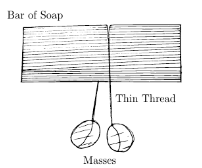
\includegraphics{./img/pressure-solid1.png}
\caption{Thin Thread}
\label{fig:pressure-solid1}
\end{center}
\end{figure}

\begin{figure}
\begin{center}
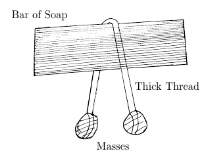
\includegraphics{./img/pressure-solid2.png}
\caption{Thick String}
\label{fig:pressure-solid2}
\end{center}
\end{figure}

\subsubsection*{Results and Conclusions}
It will be seen that the bar of soap was cut easily by using a thin thread but not by using a thick string. This because the thin thread has a small surface area and the same force and therefore a large pressure, while the thick thread has a larger area for the same force and therefore smaller pressure. 

\subsubsection*{Clean Up Procedure}
Collect all the used materials, cleaning and storing items that will be used later.

\subsubsection*{Discussion Question}
Why does a thin thread cut easily through a bar of soap while a thick thread does not?


%Pressure in Liquids


\subsection{Straw Fountain}
\begin{itemize}
\item{Preparation Time: 10 minutes}
\item{Materials: 0.5 liter water bottle with cap, water, straw, glue}
\item{Procedure: Poke a hole with the diameter of the straw in the cap of the water bottle with a hot nail or pin. Insert the straw so that it extends almost to the bottom of the water bottle and leaves enough sticking out for your mouth. Secure it with glue so that it is airtight. When the glue is dry, fill the bottle about half way with water and close the cap with the straw inside. Have a student blow as hard as they can through the straw into the water. When they run out of air and stop blowing, they will get a nice spray in the face. }
\item{Theory: By blowing into the bottle, you greatly increase the pressure inside. When you finish blowing, the pressure will try to equilibrate by forcing the pressure back out through the straw. There is nowhere for the water to go but out.}
\end{itemize}


\subsection{Cartesian Diver}

\subsubsection*{Learning Objectives}
\begin{itemize}
\item{To observe characteristics of a submerging body}
\item{To describe and apply the concept of Cartesian diver in daily life}
\end{itemize}

\subsubsection*{Background Information}
When the body is immersed in a liquid it may sink or float. The body will float in water when its density is less than density of water. A submerging body is designed in such a way that it will sink a little but also float in water. 

\subsubsection*{Materials}
Large Bottle (1.5 litres) or transparent long container with a cover or cap, water, syringe, and small stones

\subsubsection*{Preparation Procedure}
Remove the needle from the syringe.

\subsubsection*{Activity Procedure}
\begin{enumerate}
\item{Fill a bottle with some water.}
\item{Remove the plunger from the syringe and insert a few stones into the syringe.}
\item{Replace the plunger so that the syringe is full of air but sealed at the top.} 
\item{Hold the syringe upright and immerse it in the bottle making sure that the syringe and its contents float upright in the water.}
\item{Close the bottle with the cap.}
\item{Gently squeeze the bottle near the bottom.} 
\item{Observe what happens.}
\end{enumerate}

\begin{figure}
\begin{center}
\def\svgwidth{100pt}
\input{./img/cartesian-diver.pdf_tex}
\caption{The Cartesian Diver}
\label{fig:cartesian-diver}
\end{center}
\end{figure}

\subsubsection*{Results and Conclusions}
When the bottle is gently squeezed the syringe sinks down to the bottom. When the bottle is released the syringe rises back up. 

\subsubsection*{Discussion Question}
Why does the syringe move down when the bottle is squeezed?

\subsubsection*{Notes}
The syringe sinks down because the pressure in the bottle increases when you squeeze it. Added pressure will cause water from the bottle to enter into the syringe through the needle hole. This increases the weight of the syringe and thus it sinks. When the pressure is released, the water in the syringe leaves and so the syringe will float again. A Cartesian diver and a submarine use the same principle to sink and float in deep water.

	%Variation of Pressure with Depth
	
\subsection{Holey Bottle 2}
\begin{itemize}
\item{Preparation Time: 10 minutes}
\item{Materials: Water bottle, pin or small nail, water, bucket (for catching water)}
\item{Procedure: In even intervals around the base of the water bottle, poke small holes with the pin or nail. Try to get an even distribution and the same size hole all around. Fill the bottle with water and watch the water leave each hole with the same force. Blowing into the bottle will help illustrate the equality of the pressure in all directions.}
\item{Theory: Pressure in a fluid acts equally in all directions, therefore the water being forced out the bottom should feel the same amount of pressure and shoot the same distance.}
\end{itemize}


%\subsection{Holey Bottle 1}
%\begin{itemize}
%\item{Preparation time: 5 minutes}
%\item{Materials: empty 1.5 liter water bottle, water}
%\item{Construction: Pierce three or more small (less than 0.5cm) neat holes in the water bottle, at different vertical heights. An easy way to do this is to use firm but gently pressure with a metal needle from a syringe. Make sure to pierce the bottle in parts that are vertical, not parts that slope in or out.}
%\item{Procedure: Fill the bottle with water and place it on the ground or on a table. Water will pour out of the bottle through the small holes. Note that the streams of water strike the ground at different distances from the bottle. At any given time, the hole that is closest to one-half of the height of the water level should strike the ground or table at the greatest distance from the bottle.}
%\item{Theory: To understand this we must consider both Bernoulli’s Principle and Projectile Motion. Bernoulli’s Principle tells us that the horizontal speed of each stream of water varies as the square root of the depth from the surface of the water. Projectile Motion tells us that the distance reached by a stream of water is proportional to the velocity of the water and to the time before the water strikes the ground. The time before the water strikes the ground is proportional to the square root of the height above the ground. Combining these two factors, we find that the maximum distance will be reached for a stream of water that is halfway between the ground and the surface.}
%\end{itemize}


\subsection{Liquid Pressure and Depth}

\subsubsection*{Learning Objectives}
\begin{itemize}
\item{To verify the variation of pressure with depth in water} 
\end{itemize}

\subsubsection*{Background Information}
The wall of a dam is made much thicker at the bottom than at the top. Also, water storage tanks are placed at the top of a building. This is because the pressure in a liquid is related to its depth.

\subsubsection*{Materials}
Plastic bottle, nail or metal pin/needle, matches, water


\subsubsection*{Preparation Procedure}
\begin{enumerate}
\item{Light a match and heat the sharp point of the nail or pin.} 
\item{Use the heated nail to put three holes into a bottle. Put one hole near the bottom, one near the middle, and the last hole between them.} 
\end{enumerate}

\subsubsection*{Activity Procedure}
\begin{enumerate}
\item{Fill the bottle with water up to the rim.} 
\item{Hold the bottle in air using your hand or place the bottle at the top of a tall object like a stool on a table.} 
\item{Allow water to flow out of the bottle and observe the trajectory of water from each hole. Note the horizontal distance reached of water from each hole.} 
\end{enumerate}

\begin{figure}
\begin{center}
%\def\svgwidth{200pt}
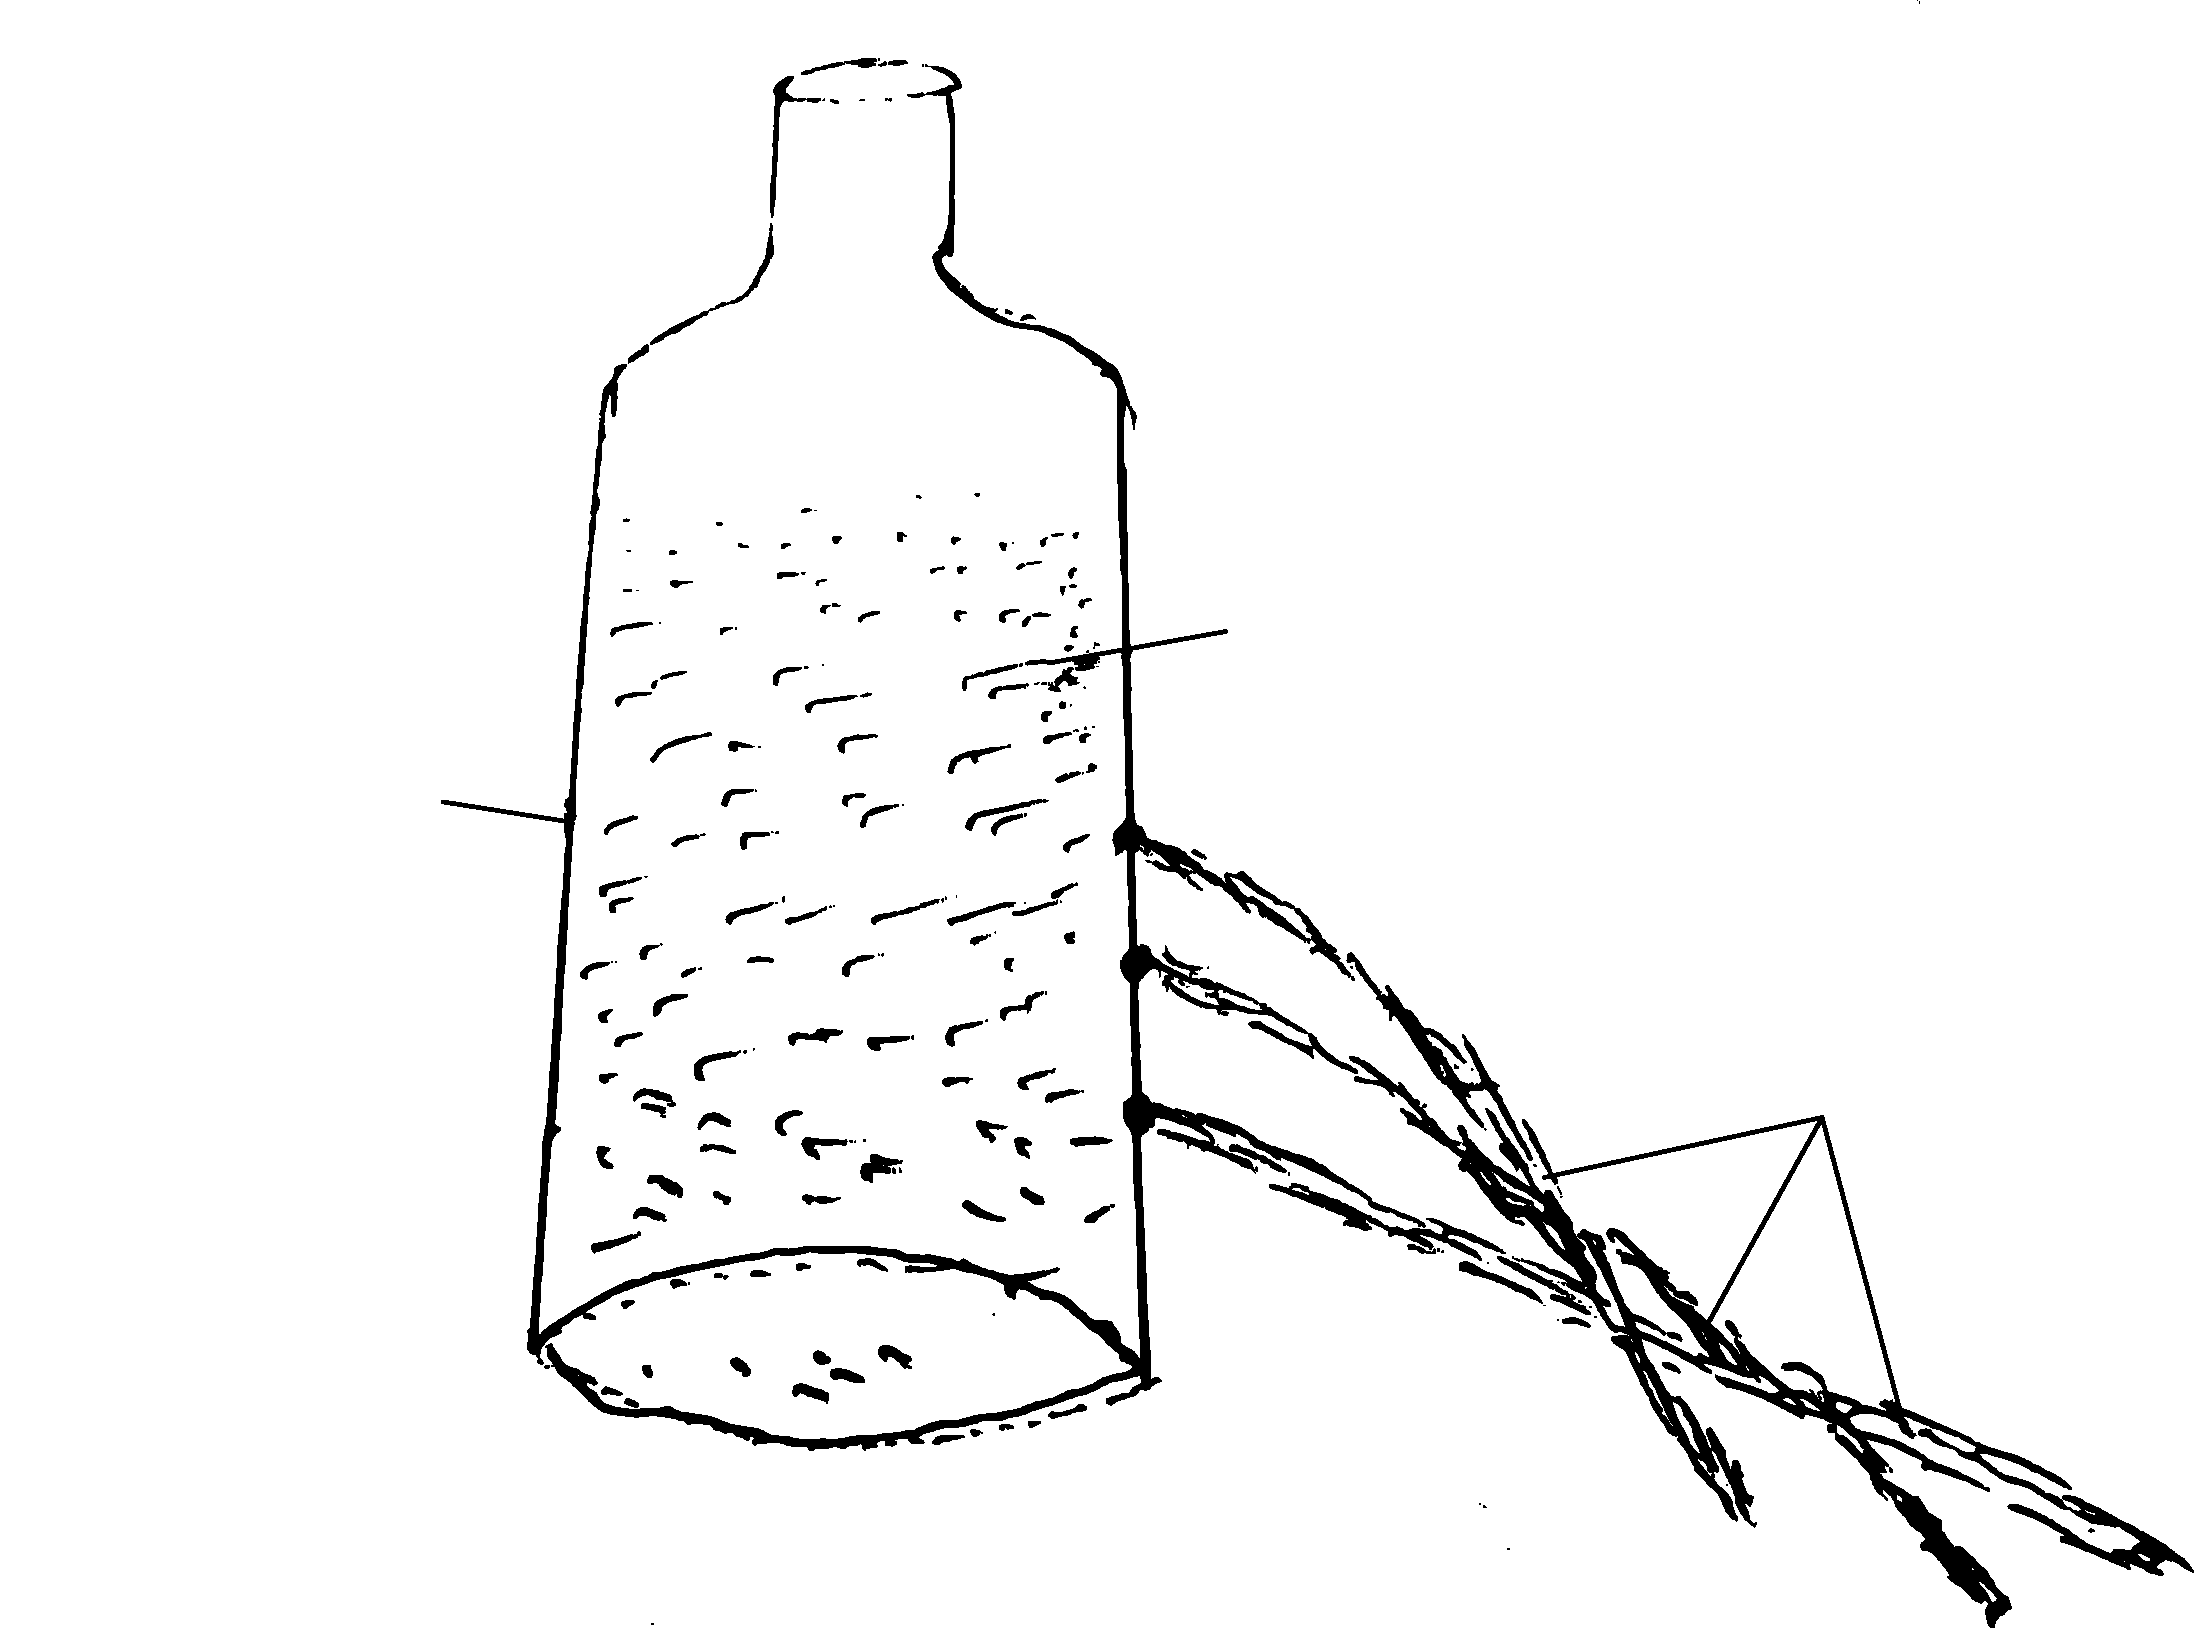
\includegraphics{./img/pressure-liquid.png}
\caption{Demonstration of the effect of depth on liquid pressure}
\label{fig:pressure-liquid}
\end{center}
\end{figure}

\subsubsection*{Results and Conclusions}
The water flows faster from the hole with the greater depth because there is greater pressure, showing that the water pressure increases with the depth of the water. This is because the weight of the water on top acts downward causing pressure. The greater the depth, the greater the weight, resulting in greater pressure. 

\subsubsection*{Clean Up Procedure}
Collect all the used materials, cleaning and storing items that will be used later.

\subsubsection*{Discussion Questions}
\begin{enumerate}
\item{What have you observed in the trajectory of water from each hole?}
\item{How does the pressure change with the depth of water? Why?}
\end{enumerate}

\subsubsection*{Notes}
There is a difference between depth and height. Height is measured from the reference point upward while depth is measured from the reference point downward. The reference point in this case is at the surface of water. 
%The holes must not be in the same vertical line in order to view the flow clearly. 	
	

	%Hydraulic Press
	
\subsection{Hydraulic Press}
\begin{itemize}
\item{Preparation Time: 15 minutes}
\item{Materials: Two syringes of different sizes (50 ml and 20 ml work well), thin rubber tubing, water}
\item{Procedure: Fill the larger syringe with water and attach one end of the rubber tubing to its end. Attach the other end of the tubing to the smaller syringe (the plunger should be inserted all the way in the smaller syringe). Pushing the plunger of the larger syringe will cause the plunger of the smaller syringe to go out, and vice-versa. You will notice that it is easier to push the plunger of the small syringe than that of the larger syringe.}
\item{Theory: Pressure is equal to force per area, and the pressure is distributed equally throughout a liquid. As such, the pressure at one plunger must be equal to the pressure at the other plunger. Setting the two ratios equal, we can see that a small force over a small area can overcome a large force over a large area.}
\end{itemize}

\begin{figure}[h!]
\begin{center}
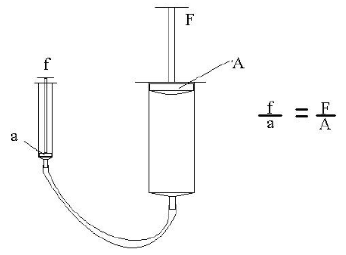
\includegraphics{./img/hydraulic-press.png}
\caption{A hydraulic press}
\label{fig:hydraulic-press}
\end{center}
\end{figure}
	

	%Manometer
	
%Atmospheric Pressure [See Gas Laws in Chem - Charles' Law]


\subsection{Atmospheric Pressure}
\begin{itemize}
\item{Preparation Time: 5 minutes}
\item{Materials: Water bottle, pin and/or nail, water}
\item{Procedure: Using an empty water bottle (bigger is better), poke four or five small holes (0.5 cm) in the bottom with the pin and then the nail. Fill the bottle about half way with water, allowing it to spill out through the holes in the bottom. While the students are watching, seal the cap on the bottle. The water will cease to pour out of the bottom despite the holes and rather predictable effect of gravity. When the gasps of wonder die down, discuss the following:}
\item{Theory: The pressure of the water combined with the pull of gravity is enough to cause the water to pour through the holes in the bottle when the cap is not sealed. When the cap is on tight, however, the combined high air pressure outside the bottle and low air pressure inside the bottle creates enough of an upward force on the water to counter the downward force of gravity.}
\end{itemize}


\subsection{Charles' Law, Part C -- Bottle Crush}
\begin{itemize}
\item{Preparation time: 10 minutes}
\item{Materials: water bottle, boiling water}
\item{Procedure: pour some boiling water into the water bottle. Cap the bottle and shake to make sure all the air in the bottle is heated from the hot water. Open the bottle and pour out the liquid. Recap the bottle. After a short time, the bottle will contract.}
\item{Theory: Charles' law states that volume is proportional to temperature. By capping the hot air inside of the water bottle, the volume of the air inside the bottle will decrease as the temperature of the gas cools off. As the volume of the air reduces, the atmospheric pressure crushes the plastic water bottle.}
\end{itemize}


\subsection{Straw Elevator}
\begin{itemize}
\item{Preparation Time: none}
\item{Materials: two straws, container, water}
\item{Procedure: Fill the container with water and insert one straw so that it stands vertically in the water. Using the other straw, blow across the opening of the vertical straw; the water level in the straw will rise.}
\item{Theory: Bernoulli’s Principle states that moving air causes low pressure; the air passing in a stream over the vertical straw creates low pressure and therefore a pressure differential between the bottom of the straw (the water) and the top. The water will move towards the lower pressure, moving up the straw.}
\end{itemize}


\subsection{Making a Magdeburg Hemisphere}

\subsubsection*{Learning Objectives}
\begin{itemize}
\item{To demonstrate the effect of atmospheric pressure} 
\end{itemize}

\subsubsection*{Materials}
Two small cooking pots of equal size, oil, matches, small pieces of paper

\subsubsection*{Preparation Procedure}
Spread oil or grease around the edge of one of the cooking pots.

\subsubsection*{Activity Procedure}
\begin{enumerate}
\item{Place some pieces of paper into the cooking pot which does not have any oil.} 
\item{Light the pieces of paper on fire.} 
\item{Allow the paper to burn until about half of it has burned.} 
\item{Place the greased cooking pot upside-down on top of the ungreased cooking pot so that they create a sort of ball and no air can escape.} 
\item{Allow the pots to cool.} 
\item{Try to separate the pots.} 
\end{enumerate}

\subsubsection*{Results and Conclusions}
After the pots have cooled it is very difficult to separate them. This is because when you burn the paper, the air in the pot expands and escapes. When you cover the pots, no more air can enter and the air inside cools, reducing the pressure inside the pots while the pressure outside the pots remains the same. The atmospheric pressure therefore presses the pots together so as to equalize the pressure on either side of the pot. 



\subsubsection*{Clean Up Procedure}
Collect all the used materials, cleaning and storing items that will be used later.

\subsubsection*{Discussion Questions}
\begin{enumerate}
\item{What is the reason for burning the paper and then covering the pot?}
\item{What happens when the pots cool?}
\end{enumerate}

\subsubsection*{Notes}
The principle behind the Magdeburg hemisphere is used to create suction. When air is heated, it expands and escapes. If the hot container is sealed and allowed to cool, the reduced number of particles causes a lower pressure than atmospherric pressure. Thus, the force pushing the two pots together from the outside is greater than the force pushing out from the inside and thus the two pots are very difficult to separate. 

	%Barometer
	
	%Siphon
	
\subsection{Siphon}
\begin{itemize}
\item{Preparation Time: 1 minute}
\item{Materials: two containers, half meter of rubber tubing/IV line/feeding tube, water}
\item{Procedure: Place one jar with water on a table and the other empty jar on a chair just below the table. Place one end of the tubing into the water and the other in your mouth. Suck on the tube until the water starts coming out and place the end of the tube into the empty beaker, holding the middle of the tube at the level of your mouth. The water will continue to flow from the water jar to the empty jar, despite the water’s initial uphill climb.}
\item{Theory: By sucking on the tubing, you create low pressure on that side. The slightly higher pressure (atmospheric) at the water will cause the water to continue to travel as long as the pressure difference is enough to overcome gravity. If you raise the middle of the tube too high, the water will stop flowing.}
\end{itemize}


%\subsection{A Siphon}
%
%\subsubsection*{Learning Objectives}
%\begin{itemize}
%\item{To demonstrate how to shift water from one bucket to another bucket using suction} 
%\item{To identify the applications of atmospheric pressure} 
%\end{itemize}
%
%\subsubsection*{Materials}
%Two buckets, water, thick rubber tube about 1 m long
%
%\subsubsection*{Activity Procedure}
%\begin{enumerate}
%\item{Pour some water into a bucket and place it on the table. Place the other bucket below the table.} 
%\item{Put the rubber tube in the bucket and fill it with water.} 
%\item{Bend one end of the tube so that air cannot enter and remove it from the bucket. Make sure the other end of the tube remains underwater.}
%\item{Lower the bent end of the tube into the lower bucket.}
%\item{Open the bent end. Observe what happens.} 
%\end{enumerate}
%
%\subsubsection*{Results and Conclusions}
%Water will flow from the bucket on the table to the other bucket below the table. This is because of the combined force of atmospheric pressure pushing in the top bucket and gravity pulling the water to the bottom bucket.
%
%\subsubsection*{Clean Up Procedure}
%Collect all the used materials, cleaning and storing items that will be used later.
%
%\subsubsection*{Discussion Question}
%If the two buckets were switched, would the water flow from the lower bucket to a bucket on the table? Explain your answer.
%
%\subsubsection*{Notes}
%The flow of water is driven by the net difference in elevation of the two ends of the tube. The force of gravity pulls the water through a siphon. As long as the inlet is above the outlet, water will flow even if it has to go up before it goes down. This is because as water is pulled down the of the tube by gravity the pressure decreases at the top of the siphon and air pressure in the bucket pushes the water into the tube. This will continue until the water level in the top bucket is below the inlet of the tube.	
	

\subsection{Automatic Flushing Tank}

\subsubsection*{Learning Objectives}
\begin{itemize}
\item{To identify the application of pressure differences}
\end{itemize}

\subsubsection*{Background Information}
The effect of pressure in a liquid can be observed in different ways. Automatic flushing tanks operate under the influence of pressure in a liquid. When the level of water in a container reaches the highest point in the exit pipe, water will drain from the tank until the level of the water in the tank is below the level of the outlet. The tank can then be refilled to repeat the cycle. This type of system is useful for flushing or when you need a certain amount of water for a given amount of time.

\subsubsection*{Materials}
Empty drinking water bottle, straw, water, bucket, chewing gum OR superglue

\begin{figure}
\begin{center}
\def\svgwidth{100pt}
\input{./img/auto-flushing-tank.pdf_tex}
\caption{The Automatic Flushing Tank}
\label{fig:auto-flushing-tank}
\end{center}
\end{figure}

\subsubsection*{Preparation Procedure}
Cut off the top of an empty water bottle, make a hole at the bottom so as to fit the straw through it. 
Bend the straw inside the bottle so that it makes an upside down 'U' shape. Use the chewing gum or superglue to seal the hole.

\subsubsection*{Activity Procedure}
\begin{enumerate}
\item{Hold the bottle and place the bucket below the bottle.} 
\item{Pour some water into the bottle up to and above the bend in the straw and observe what happens.} 
\end{enumerate}

\subsubsection*{Results and Conclusions}
The water will flow into the bucket through the bent straw. 

\subsubsection*{Clean Up Procedure}
Collect all the used materials, cleaning and storing items that will be used later.

\subsubsection*{Discussion Question}
What causes the water to flow from the bottle to the bucket? How does this work?

\subsubsection*{Notes}
The siphon principle states that liquid is able to flow without pumping because the combined pressure of the water and the atmosphere pushing down on the water is greater then the air pushing up on the straw. The automatic flushing tank does not require a handle to trigger the flush. Once the water flows into the tank up to the level of the siphon, the tank will flush automatically. 
	
	
	
	%Pumps (Lift Pump, Force Pump, Bicycle Pump)


\subsection{Reverse Air Pump}
\begin{itemize}
\item{Preparation Time: varies, about 1 hour}
\item{Materials: Bicycle pump (the tall, metal kind), short piece of rubber tubing fitted to pump valves, utility knife, tightening sleeves, extra valve}
\item{Procedure: There are two parts of the pump that control the direction of airflow: the first is a diaphragm inside the pump and the second is a ball valve at the base of the pump in the hose.
\begin{enumerate}
\item{You need to open the pump and pull out the ‘dipstick’ with the diaphragm attached. At the bottom, there should be a diaphragm with holes around the top, a metal disc the same diameter as the diaphragm, and a few nuts and washers to keep it all together. In its normal configuration, the diaphragm is pulled down by friction away from the disc when the pump handle is pulled up, allowing air to enter the pump freely. When the pump handle is pushed in, the diaphragm is forced against the disc, restricting any back airflow, and forcing all the air forward through the hose. Switch the position and direction of the diaphragm and disc so that it has the opposite effect when the pump handle is pulled in or out.}
\item{Next, you need to cut open the hose at the base of the pump and find the valve with the small bead inside. Normally, when air is forced forward through the valve, the bead does not restrict any airflow. When air tries to go back through the pump, the bead blocks the valve and stops any airflow. Switch the direction of the valve.}
\item{From here, you need to reattach the hose to the pump. You may need to get another nozzle to attach to the pump, attaching the hose with reversed valve with the extra bit of rubber tubing. It depends on your pump, but if you have made it this far, you will find a way to make it work. Tightening sleeves will come in handy here to make sure no air is lost after all this cutting and jury-rigging.}
\end{enumerate}
} % Procedure
\item{Applications: This suction pump is great for showing the gas laws and boiling points: suck the air out of a jar of water and watch the water boil, you could also kill stuff in the jar this way, but that is just morbid, and possibly cool, or that sound travels through a medium.}
\end{itemize}

%\section{Work, Energy and Power}

%Work


\subsection{Work as Heat, Part A}
\begin{itemize}
\item{Preparation time: 5 minutes}
\item{Materials: thin strip of metal, pliers}
\item{Procedure: Take a piece of metal. Use a set of pliers to bend the metal back and forth. Feel the temperature of the metal.}
\item{Theory: Work can manifest itself in a variety of ways. One of the most common ways is the rise in temperature. By moving the metal back and forth, you are doing work on the metal. This work is converted into heat. This heat is evidenced by the rise in temperature in the metal. }
\end{itemize}

\subsection{Work as Heat, Part B}
\begin{itemize}
\item{Preparation time: 0 minutes}
\item{Materials: radio antennas, old or new }
\item{Procedure: The radio antennas operate in a telescopic motion. Pull the radio antenna in and out for one full minute. Do not break the antenna in this movement. Observe the temperature of the antenna after the work is over.}
\item{Theory: Again, you are doing work on the radio antenna by moving it in an out quickly. Through this action, the antenna heats up. This is the evidence of the work you have been doing. Work is defined as force times distance or. In this case, the force is the effort required to move the antenna in and out while the distance is the length of the antenna.}
\end{itemize}

\subsection{Work as Light}
\begin{itemize}
\item{Preparation time: 0 minutes}
\item{Materials: duct tape, or other tape that holds together tightly.}
\item{Procedure: Cut two pieces of duct tape. Press the ends of the bottom pieces of tape together but allow the top pieces of tape to be apart. Hold tightly to both pieces of tape at the top, and quickly rip them apart. Observe the blue light when the tape comes apart.}
\item{Theory: Pulling the tape apart quickly creates a faint blue light. It is best to observe this light at night since it is so faint. In this activity, this is the work being done to pull the tape apart. Unlike the previous activities, this work is released as light. This phenomenon as where work manifests itself as light is called triboluminescence. This is the same phenomenon that causes the green light when snapping wintergreen mints.}
\end{itemize}


%Energy

	%Kinetic Energy, Potential Energy
	
	%Transformation of Energy
	
	%Conservation of Energy
	
	
%\subsection{Pencil Launcher}
%\begin{itemize}
%\item{Preparation Time: 5 minutes}
%\item{Materials: Clothes clip, thread, two pencils}
%\item{Procedure: Open the clip and tie the closed end with thread so that the clip stays open against the tension of the spring. Place the clip flat on a table and place two pencils next to the clip, one on either side, so that the eraser touches the tied end and the tips point out in opposite directions along the table. Cut the thread holding the clip open and stay clear of the flying pencils.}
%\item{Theory: The spring inside the clip holds energy when it is forced to contract. When the clip is allowed to close, the potential energy of the spring is transformed into mechanical energy as the clip moves, forcing the pencils away at a decent speed.}
%\end{itemize}


\subsection{Potential Energy of a Spring}

\subsubsection*{Learning Objectives}
\begin{itemize}
\item{To observe the change in energy from potential to kinetic}
\end{itemize}

\subsubsection*{Background Information}
In a closed system, where no force acts on the objects, the total energy remains constant.  In the case of mechanical energy, this means that potential energy and kinetic energy can change, but their total remains the same.  Springs and other elastic materials also have potential energy in the form of elastic potential.

\subsubsection{Materials} 
Clothes pin, thread, two pencils

\begin{figure}[h]
\begin{center}
\def\svgwidth{100pt}
\input{./img/energy-conservation.pdf_tex}
\caption{Energy conservation in a spring}
\label{fig:energy-conservation}
\end{center}
\end{figure}

\subsubsection{Activity Procedure}
\begin{enumerate}
\item{A clothes pin has two ends: one for gripping clothes and one for pushing with fingers. Press the finger ends together so the gripping end is open as far as possible. Use a thread to tie the finger ends together so that the gripping ends stay wide open.}
\item{Place the clothes pin side-down on a table and place two pencils touching the clothes pins as shown in the figure below.}
\item{Cut the thread holding the clothes pin open, the clothes pin should open quickly and push the pencils away.}
\end{enumerate}

\subsubsection*{Cleanup Procedure}
Return all materials to their proper places.

\subsubsection*{Discussion Questions}
\begin{enumerate}
\item{What two types of energy are being used here?}
\item{Describe the change in energy occurring here.}
\end{enumerate}
 
\subsubsection{Notes}
The spring inside the clip holds energy when it is forced to contract.  
When the clip is allowed to close, the potential energy of the spring
is converted into mechanical energy as the clip moves, forcing the pencils
away quickly.

The interconversion of potential and kinetic energy may also be shown with a simple pendulum. Another option is to hold a heavy book above the table and then to drop it on the table.


%Power
%\section{Light}

%Propagaion and Transmission of Light

	%Rays (straight line)
	
	
	\subsection{Light in a Straight Line}

\subsubsection*{Learning Objectives}
\begin{itemize}
\item{To explain the concept of light rays and beam of light} 
\item{To demonstrate that light travels in straight line} 
\end{itemize}

\subsubsection*{Materials}
Torch/kerosene lamp/light source, cardboard, 6 large books, iron nail

\subsubsection*{Preparation Procedure}
Cut 3 rectangular pieces of cardboard. Make a hole at the center of each piece of cardboard using a nail. The holes should all be the same distance from the bottom of the cardboard so they can be easily aligned.

\begin{figure}[h!]
\begin{center}
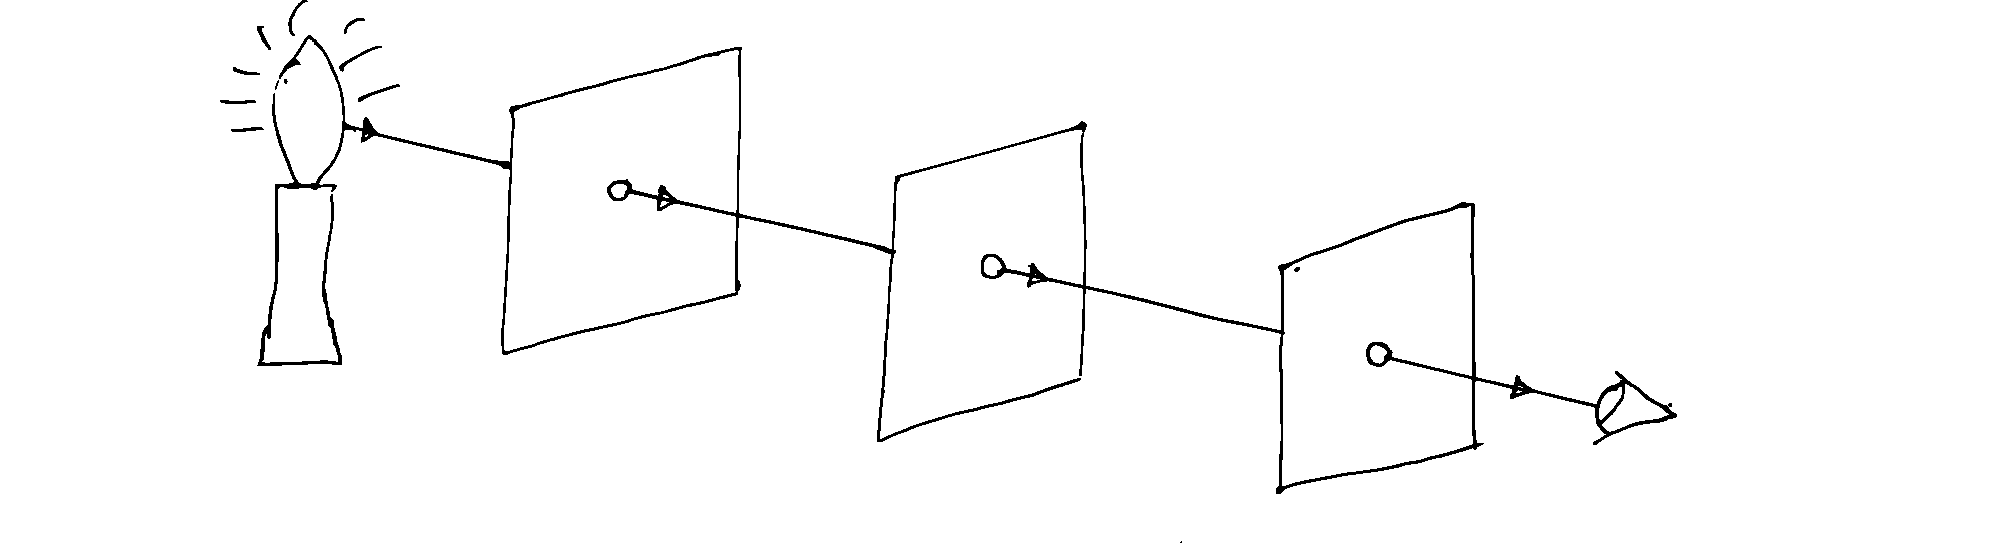
\includegraphics{./img/prop-of-light.png}
\caption{Experiment to show that light travels in straight lines}
\label{fig:prop-of-light}
\end{center}
\end{figure}

\subsubsection*{Activity Procedure}
\begin{enumerate}
\item{Arrange the cardboard pieces in between two books so they stand upright and arrange them in a straight line. The cardboard pieces should be at least 45 cm apart so that the holes are aligned.} 
\item{Place a light source 30 cm from the first piece of cardboard. Have an observer stand at the other end of the table.} 
\item{Look through the series of holes to see the light source.}
\item{Slightly displace one of the pieces of cardboard and again look through the holes.}
\end{enumerate}

\subsubsection*{Clean Up Procedure}
Collect all the used materials, cleaning and storing items that will be used later.

\subsubsection*{Discussion Questions}
\begin{enumerate}
\item{What does this experiment show about the way that light travels?}
\item{Draw a ray diagram to show the two alignments of the cardboard pieces.}
\end{enumerate}

\subsubsection*{Notes}
This activity is best done at night or in a dark room so that the light can be seen clearly through the holes.


%\subsection{Pinhole Camera}
%\begin{itemize}
%\item{Preparation Time: half hour}
%\item{Materials: Cardboard box, black paint if necessary, translucent screen (tissue paper, color gel, etc.), pin, tape, scissors, light source, any object}
%\item{Procedure: Cut out one side of the cardboard box and paint the inside black. Replace the cutout side of the box with your translucent screen, taping it shut along all four edges. On the opposite side of the box from the screen, poke a small hole with the pin. Your camera is now complete.\\
%In a dark room, shine a bright light source on an object and aim the camera at it so that the light from the object passes through the pinhole to the screen. If the source is bright enough, the image should appear, upside down, on the screen. Play around with the object distance until you have a large, clear image on the screen. It is recommended to try this outside on a bright day, but you will need to cover the space between the camera and your head completely so that no light can enter.}
%\item{Theory: Light travels in a straight line, and so light from the top of the object will pass at an angle through the pinhole, appearing at the bottom of the screen on the other side. Alternately, light from the bottom of the object will appear at the top of the screen. A strong light source is needed because the aperture pinhole is small and will only admit a small amount of light.}
%\end{itemize}
%
%\begin{center}
%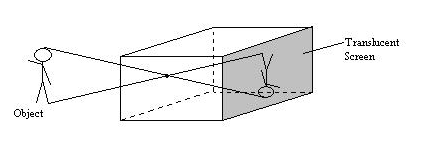
\includegraphics[width=8cm]{./img/pinhole-camera-1.png}
%\end{center}


\subsection{Pin Hole Camera}

\subsubsection*{Learning Objectives}
\begin{itemize}
\item{To construct a pinhole camera.}
\item{To use a pinhole camera to demonstrate that light travels in a straight line.}
\end{itemize}

\subsubsection*{Background Information}
Light rays travel in a straight line.  When the rays of light from a source pass through a small hole, the image of the source (any object producing or reflecting light) can be seen inverted on the other side of the hole.  A simple, closed box can be used to demonstrate this property of light.  This instrument is called a pinhole camera and it demonstrates the basis of photography.

\subsubsection*{Materials}
Cardboard box, plain paper, candle, kerosene, pin, glue, matches


\subsubsection*{Preparation Procedure}
\begin{enumerate}
\item{Remove one side of an empty box and on the opposite side make a small hole using a pin.} 
\item{Soak a piece of plain paper in kerosene to make it translucent.} 
\item{Using glue, cover the open side of the box with the translucent paper to act as a screen.} 
\item{Light the candle.} 
\end{enumerate}

\begin{figure}
\begin{center}
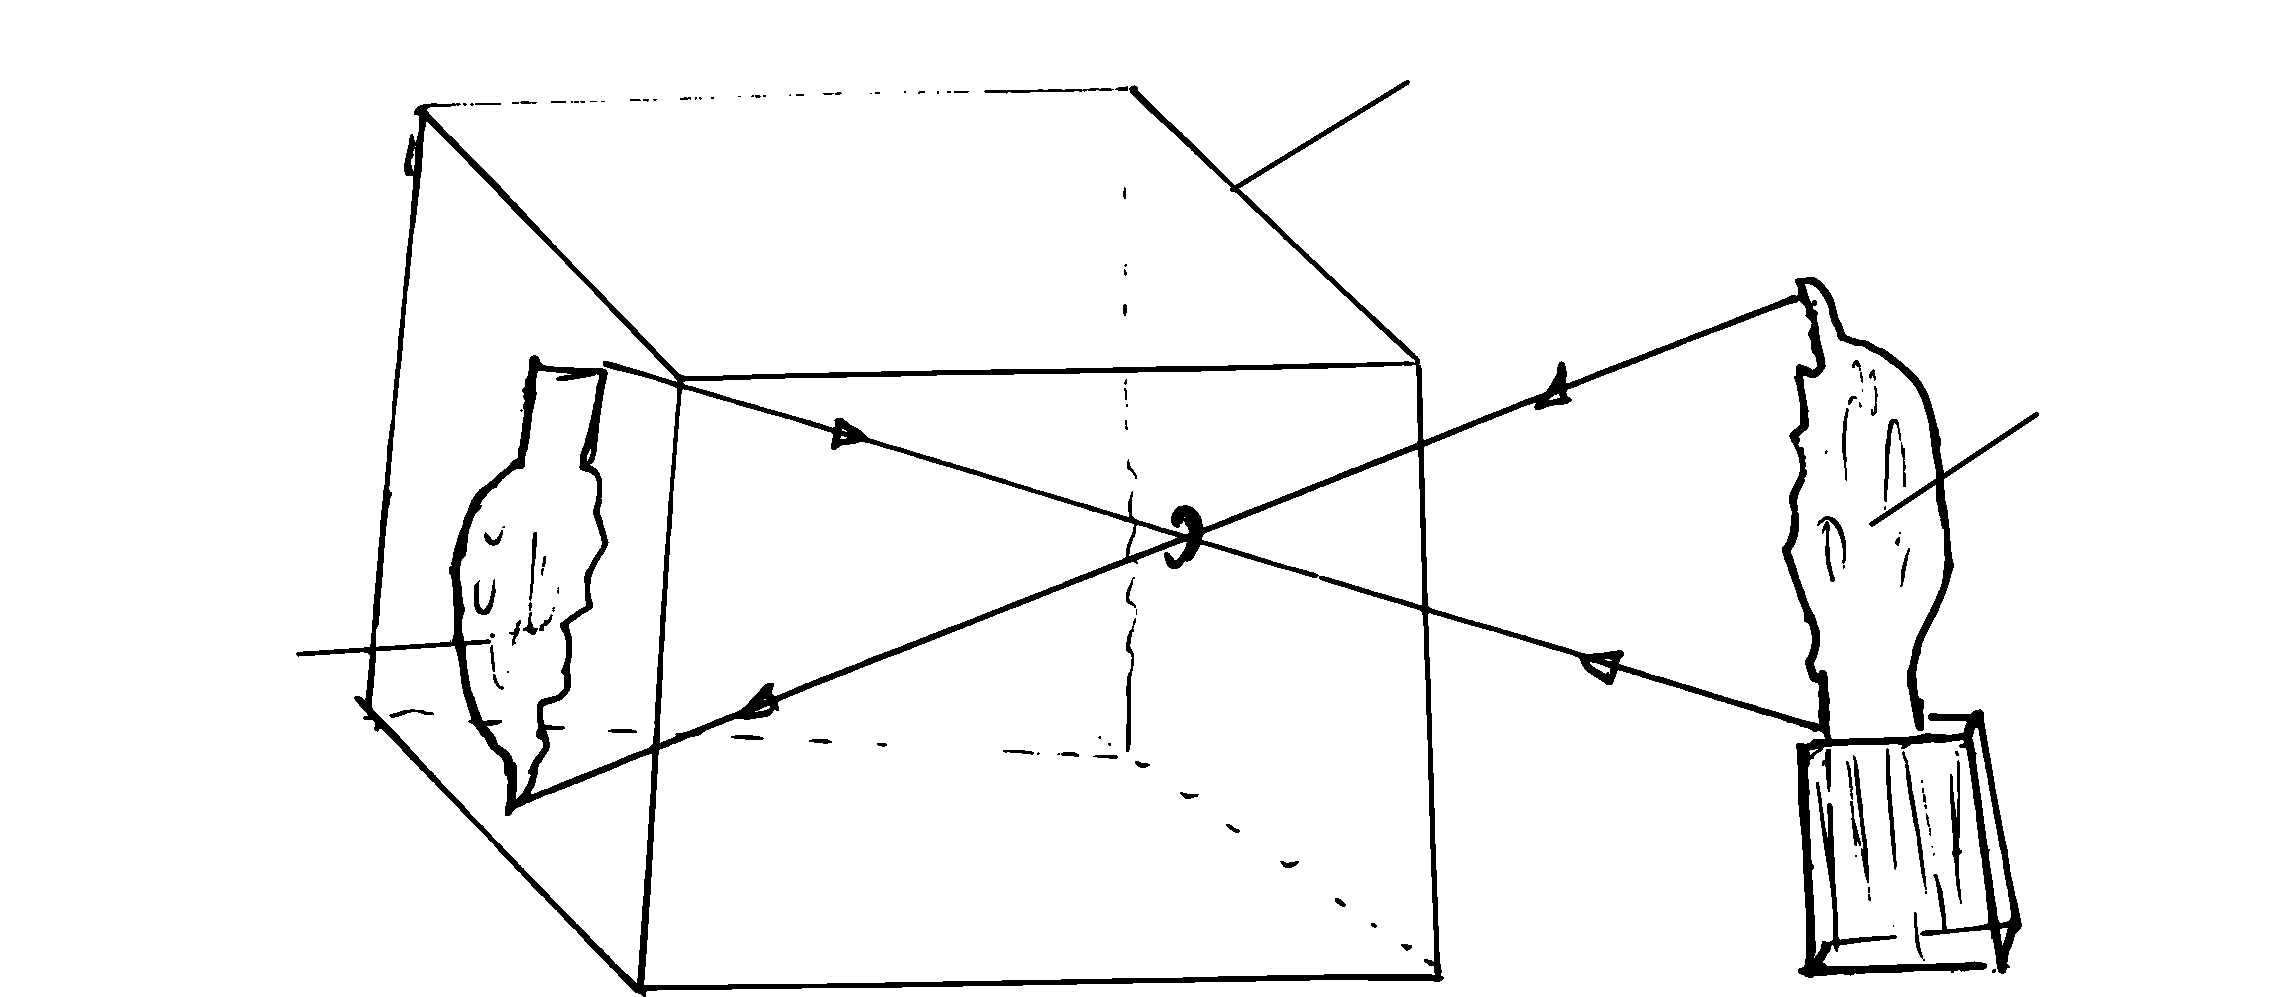
\includegraphics{./img/pinhole-camera.png}
\caption{Construction of a pinhole camera}
\label{fig:pinhole-camera}
\end{center}
\end{figure}

\subsubsection*{Activity Procedure}
\begin{enumerate}
\item{Place the candle in front of the box on the side with the small hole.} 
\item{Observe and record the image of the candle on the plain paper.} 
\end{enumerate}

\subsubsection*{Results and Conclusions}
Rays of light travel in a straight line. The observed image is inverted as the result of the path of light rays from the object to the paper -- the rays cross at the pin hole.

\subsubsection*{Clean Up Procedure}
The pinhole camera can be stored for later use.

\subsubsection*{Discussion Questions}
\begin{enumerate}
\item{What properties of light allow the image to appear?}
\item{Why is the image of the candle inverted?}
\item{Draw a ray diagram to represent how a pinhole camera works.}
\end{enumerate}

\subsubsection*{Notes}
The hole must be very small, clean for the pin hole camera to work properly. A large or jagged hole will create a blurred image.  
If it is difficult to see the image go to a darker room or try the experiment in the evening or night.


\subsection{Light through a Comb}
\begin{itemize}
\item{Preparation Time: 1 minute}
\item{Materials: comb, light source, optional mirror}
\item{Procedure: In a dark place, shine the light parallel to a table surface through the comb. The apertures in the comb will act as ‘beams’ of light. Reflect the beams off a mirror and observe the straight-line propagation of light.}
\item{Theory: Light travels in a straight line, even when reflected at a surface.}
\end{itemize}

	
	%Shadows
	
	
%Laws of Reflection (reflection of light)


\subsection{Laws of Reflection}

\subsubsection*{Learning Objectives}
\begin{itemize}
\item{To verify the laws of reflection in a plane mirror}
\end{itemize}

\subsubsection*{Materials}
Plane mirror, pins, thick cardboard, protractors and rulers, white paper, pen, pencil

\subsubsection{Activity Procedure}
\begin{enumerate}
\item{Place a plane mirror vertically on a sheet of white paper on top of the cardboard.}
\item{Draw a line along the back of the mirror.}
\item{Construct a perpendicular line to the line on which the mirror stands.}  
\item{Draw a line making an angle of incidence $i$ from the normal.}
\item{Insert two pins on the line drawn which makes an angle $i$ with the normal.}
\item{Look into the mirror such that the images of the pins look as if they are in straight line.}
\item{Insert two more pins so that they are in line with the images of the first two pins.  These two more pins mark the path of the reflected ray.}
\item{Remove the pins and draw lines joining the marks of the pins.}
\item{Using a protractor measure and record the angle between the reflected ray and the normal.}
\end{enumerate}

\subsubsection*{Results and Conclusions}
This practical is used to verify the Laws of Reflection and to observe and describe images formed in a plane mirror.  It will be seen that the angles of reflection are equal to the angles of incidence in each case.



%Applications (periscope, telescope)


\subsection{Kaleidoscope}
\begin{itemize}
\item{Preparation Time: 5 minutes}
\item{Materials: 3 or more mirrors of equal size OR 3 or more pieces of glass of equal size with metal foil on one side, tape; Optional: colored objects}
\item{Procedure: Tape the three mirrors together so that they form a triangular tube with the reflective sides facing in. Look through the kaleidoscope at any objects, especially colored beads or paper, and turn the scope to watch the pretty colors change!}
\end{itemize}

%%\section{Introduction to Physics} 

\begin{multicols}{2}


\section*{Concept of Physics} \index{Physics! concept of}


%\subsection{•}

\begin{center}
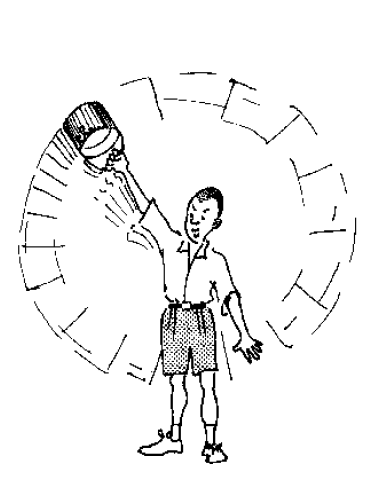
\includegraphics[width=0.45\textwidth]{./img/source/bucket-swing-2.png}
\end{center}

%\begin{description*}
%%\item[Subtopic:]{}
%\item[Materials:]{}
%\item[Setup:]{}
%\item[Procedure:]{}
%\item[Hazards:]{}
%\item[Questions:]{}
%\item[Observations:]{}
%\item[Theory:]{}
%\item[Applications:]{}
%\item[Notes:]{}
%\end{description*}

A bucket of water is sufficient to start investigating the effect of centripetal forces. Fill the
bucket with various quantities of water and you will learn even more by doing. Increase the
number of revolutions of the bucket.\\

Physics must not be a boring, tough subject, just good for exams and to be understood by a
few ``experts'' only. Physics should not happen in books only. It is everywhere where things
are. The teaching of science without experiments is just like a ngoma without dancers.\\

Pupils learn more and better by doing. Stimulate them to investigate their environment
through easy to carry out experiments. Ask the pupils to make a list of physical phenomena
which can be observed in their environment. Let the pupils enjoy physics. The activities in this book
show how this can be achieved.

\vfill
\columnbreak


%==================================================================================================%

\section*{Applications of Physics} \index{Physics! applications of}


\subsection{Measurement and Data} \index{Measurement! introduction}

\begin{center}
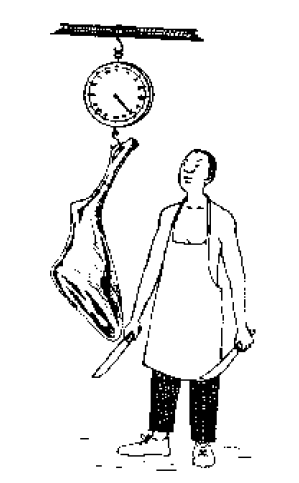
\includegraphics[width=0.4\textwidth]{./img/source/butcher.png}
\end{center}

Imagine you would buy different kinds and different quantities of meat. The butcher will have
to weigh and then calculate the price for each kind of meat and produce the total bill. Thus,
measuring and the collection of data happen everyday in our life.\\

The tailor takes the measurements of his customer and of the material needed for a suit. The
milkman measures the volume of the milk sold. The technician measures with a caliper the
diameter of a screw and even at school the time of each period is measured. Especially in
engineering precise measurements are indispensable.

\vfill
\columnbreak

\subsection{Mechanics} \index{Mechanics}

\begin{center}
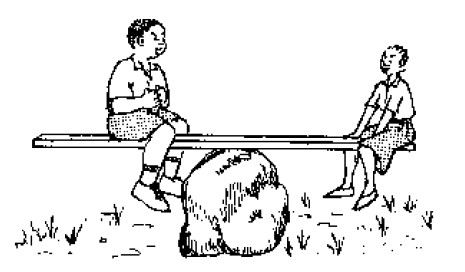
\includegraphics[width=0.4\textwidth]{./img/source/mechanics.png}
\end{center}

Have you observed children balancing a plank like a seesaw? They know how a big and a
small child can balance although they are of different weight.\\

Usually they do not know what a fulcrum, a load distance and a moment of force is. However,
such basic mechanics dominate an essential part of our daily life. We encounter motion,
friction, inertia, work and power almost every day. We also learn in a practical way about
density, pressure of fluids or gases. Work, energy, power and other physical phenomena look
very abstract in books but happen every day. Also the movement of earth, moon and the
planets which determines the lengths of our days, months and years, has to do with basic
mechanics such as motion, mass attraction and centripetal forces.

\subsection{Matter} \index{Matter! introduction}

\begin{center}
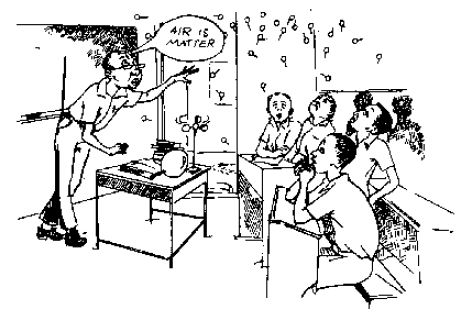
\includegraphics[width=0.4\textwidth]{./img/source/matter.png}
\end{center}

A chair can be touched. Water in a bucket also. But air? Can you imagine that while you are
reading these lines your nose is punched more than 100 billion times by air molecules?\\

The environment around us, whether in solid, liquid or gaseous state is made up of billions of
tiny particles which are either molecules or atoms. These particles which constitute air are so
tiny, that we cannot see them even by a powerful microscope. However, the students can be
given an idea of the particle structure of matter by indirect evidence.

\subsection{Thermal Physics} \index{Thermal physics! introduction}

\begin{center}
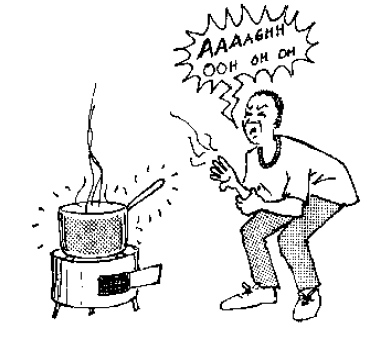
\includegraphics[width=0.4\textwidth]{./img/source/thermal-physics.png}
\end{center}

Would you ever touch the handle of a hot pan? Would you put margarine just aside
of the pot? Would you hold your hand right above the hot water? No; this is
because we know a lot about thermal physics by daily experience. But we do not always
relate this knowledge with what we learn at school about heat conduction, heat radiation or
heat convection as is the case in the examples mentioned above.\\

Thermal physics has also to do with thermal energy and the measurement of temperatures,
with calorimetry, change of states, expansion, etc. Ask the students to talk about everyday
thermal phenomena and to write about these. Why should we teach this topic by talk and
chalk only, if there are illustrative experiments which do not require a lot of equipment and
which are not time consuming in their preparation and performance?

\subsection{Wave Motion} \index{Waves! introduction}

\begin{center}
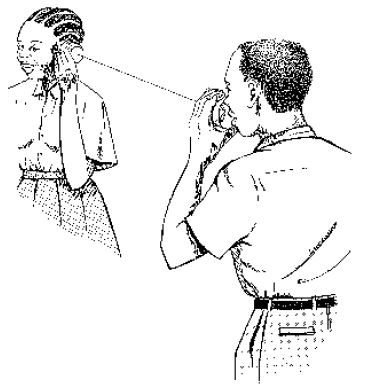
\includegraphics[width=0.4\textwidth]{./img/source/wave-motion.jpg}
\end{center}

Communication through spoken words has to do with the transport of waves. Telephone and
radio are well known. But do we think about waves when we hear a music band, when a crow
is croaking or when children are playing with a string telephone? All this is everyday knowledge about the transport of sound waves.\\

But teaching about waves does not mean only sound waves. Water waves we notice in a puddle as well as in a cup of tea. Electromagnetic waves are responsible for hearing our radios and watching our televisions.
Produce waves in physics not only by talking. Meaningful and simple experiments are
possible on many themes of this topic. No time? Hand experiments are always brief,
illustrative and can be carried out with everyday things.

\subsection{Light and Optics} \index{Light! introduction}

\begin{center}
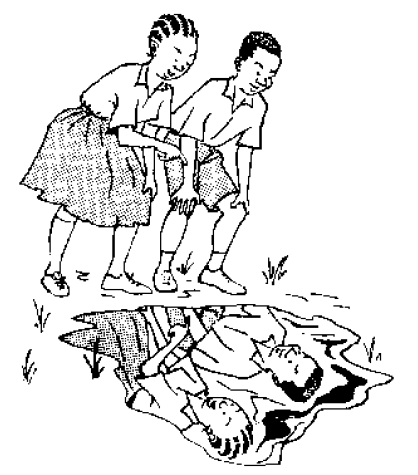
\includegraphics[width=0.4\textwidth]{./img/source/light-optics.png}
\end{center}

When we hear about optics, the optician, eye glasses and lenses come into our mind. But that
is not all what optics is about. Optics is also about the reflection of an image in a mirror or in a
water puddle. The water surface is like a mirror. The image to be seen is inverted and it
seems to be as far behind the water surface as the object is in front of it.\\

Perhaps there are no curved mirrors at your school to teach about concave and convex mirrors. No problem. Take a polished spherical spoon and you will be able to perform an interesting lesson. Certainly not all themes can be taught by simple qualitative hand experiments only. But you may be astonished to see how many there are for eye catching demonstrations.

\subsection{Electricity and Magnetism} \index{Electricity! introduction} \index{Magnetism! introduction}

\begin{center}
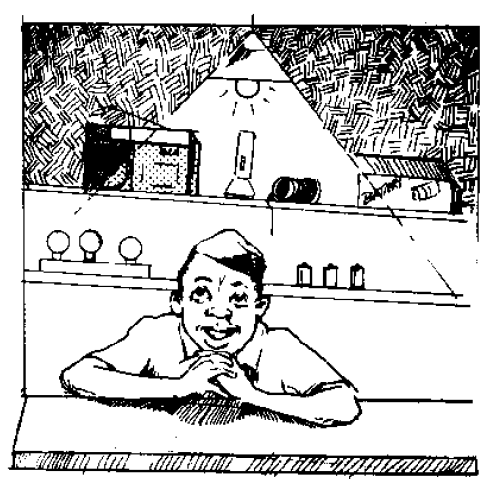
\includegraphics[width=0.4\textwidth]{./img/source/elec-mag.png}
\end{center}

Effects of electricity can be observed nowadays nearly everywhere. A light bulb lights the
room; a radio enchants our ears; a torch helps to find our way in the darkness; and last but
not least we do owe a cool soft drink to a refrigerator. The understanding on how electric
apparatus work is essential nowadays.\\

But electricity does not only mean a current flows in a circuit. It means also static electricity or lightning during a thunderstorm. The topic of electricity is closely related to magnetism.
Without magnets electric motors would not work. Loudspeakers work with magnets and even
a simple bicycle dynamo has one. In harbours you can see how ``attractive'' magnets can be
to lift heavy loads. Do you think that the teaching of electricity by doing is difficult, needs a lot
of equipment and is even dangerous? See that this is not the case by trying some of the activities provided in this manual.

%==================================================================================================%


\end{multicols}

\pagebreak
%%\section{Introduction to Laboratory Practice}

\begin{multicols}{2}


%==================================================================================================%

\section*{Laboratory Rules and Safety}


\subsection{Display of Hazardous Chemicals}

\begin{center}
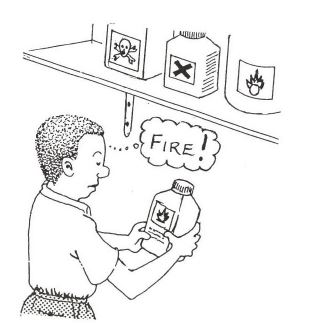
\includegraphics[width=0.45\textwidth]{./img/source/display-chemicals.jpg}
\end{center}

\begin{description*}
%\item[Subtopic:]{}
%\item[Materials:]{}
%\item[Setup:]{}
\item[Procedure:]{Display some well labelled containers with
hazard symbols for the students and let them
talk about them.}
%\item[Hazards:]{}
%\item[Questions:]{}
%\item[Observations:]{}
%\item[Theory:]{}
%\item[Applications:]{}
%\item[Notes:]{}
\end{description*}

\subsection{A Safety Game}

\begin{center}
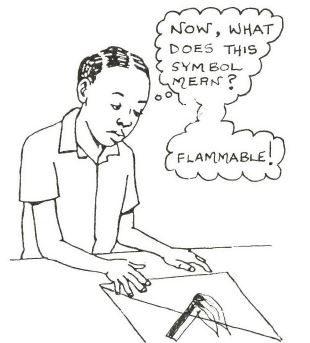
\includegraphics[width=0.45\textwidth]{./img/source/safety-game.jpg}
\end{center}

\begin{description*}
%\item[Subtopic:]{}
\item[Materials:]{Cards of hazard symbols}
%\item[Setup:]{}
\item[Procedure:]{Play a game with the symbol charts. A
student is given a hazard symbol. He has to
explain the hazard shown and to explain the
necessary safety precautions in order to avoid
that hazard.}
%\item[Hazards:]{}
%\item[Questions:]{}
%\item[Observations:]{}
%\item[Theory:]{}
%\item[Applications:]{}
%\item[Notes:]{}
\end{description*}

\columnbreak

\subsection{The Cleanliness Play}

\begin{center}

\includegraphics[width=0.45\textwidth]{./img/source/cleanliness-play.jpg}
\end{center}

\begin{description*}
%\item[Subtopic:]{}
%\item[Materials:]{}
%\item[Setup:]{}
\item[Procedure:]{Ask the students to play group-wise short
and funny scenes using appropriate words to
make them familiar with cleanliness rules.}
%\item[Hazards:]{}
%\item[Questions:]{}
%\item[Observations:]{}
%\item[Theory:]{}
%\item[Applications:]{}
%\item[Notes:]{}
\end{description*}

\subsection{The Tidiness Play}

\begin{center}
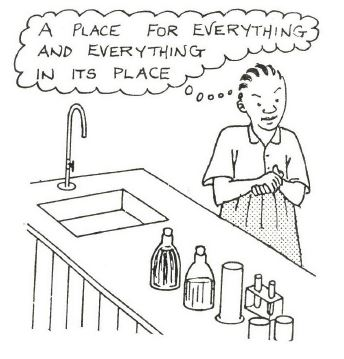
\includegraphics[width=0.45\textwidth]{./img/source/tidiness-play.jpg}
\end{center}

\begin{description*}
%\item[Subtopic:]{}
%\item[Materials:]{}
%\item[Setup:]{}
\item[Procedure:]{Chemists are very tidy. Apparatus and
reagents should be arranged on the table so that
they can be reached easily but at a safe distance
from the experiment.}
%\item[Hazards:]{}
%\item[Questions:]{}
%\item[Observations:]{}
%\item[Theory:]{}
%\item[Applications:]{}
%\item[Notes:]{}
\end{description*}

\end{multicols}

\pagebreak

%==================================================================================================%

\section*{The Scientific Method}
\label{sec:scientific-method}

\setcounter{secnumdepth}{1}

The following activities can be used as a method of introducing students to the scientific method. Rather than just performing the activities, first identify the question or problem with the students, then have them form a hypothesis for each step of the experiment. Students should record observations and data accordingly and use them to draw a conclusion about the activity.\\

Prepare an activity sheet for each student or have them copy it into their notebooks before performing the activities. Set up stations for the various activities and have students rotate among them in small groups. Incorporate activities in Biology and Chemistry as well from the \emph{Shika na Mikono} resource manual.\\


\subsection{Complete the Circuit}

\begin{center}
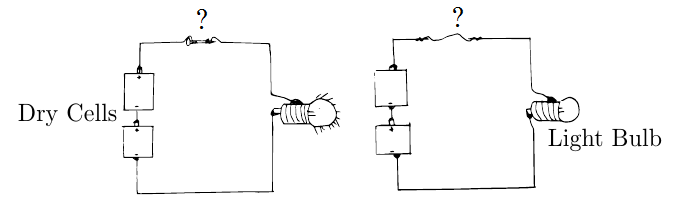
\includegraphics[width=0.8\textwidth]{./img/conductors-insulators-sci-meth.png}
\end{center}

\begin{description*}
\item[Materials:]{Dry cell, speaker wire, bulb/ammeter, cardboard, various objects, e.g. rubber band, nail, paper, aluminum foil, toothpick, pen, scissors, bottle cap, coin, balloon, chalk}
\item[Setup:]{Connect a dry cell and bulb in series using speaker wire and attach to a sheet of cardboard. Leave two wires free and pin to the cardboard to act as a switch.}
\item[Problem:]{Which objects will light a bulb?\\

\begin{tabular}{|l|c|c|} \hline
\multirow{2}{*}{\textbf{Object}} & \textbf{Hypothesis} & \multirow{2}{*}{\textbf{Experimental Result}} \\
& \textbf{(Light or No Light)} & \\ \hline
Copper wire & & \\ \hline
Pen & & \\ \hline
Aluminum foil& & \\ \hline
Paper& & \\ \hline
Nail& & \\ \hline
Toothpick& & \\ \hline
Bottle cap& & \\ \hline
Balloon& & \\ \hline
Chalk& & \\ \hline
Scissors (blade)& & \\ \hline
Scissors (handle)& & \\ \hline
\end{tabular}\\[10pt]
}
\item[Hypothesis:]{Predict which materials will cause the bulb to light when placed across the switch. Record predictions in the table.}
\item[Procedure:]{Test each object by placing it across the free wires to close the circuit.}
\item[Observations:]{Record the result for each item in the table.}
\item[Questions:]{}\hfill 
\begin{enumerate}
\item Which materials caused the bulb to light?
\item These objects are made from what kind or materials?
\item What other objects in the room can you find to test? Will they light the bulb?
\end{enumerate}
\item[Theory:]{\emph{Conductors} are materials which easily allow electrons to flow through them. \emph{Insulators} are materials which do not easily allow the the flow of electrons. Examples of good conductors are most metals, water and the human body. Examples of good insulators are rubber, wood and plastic.}
\end{description*}

\pagebreak


\subsection{Density Tower}

\begin{center}
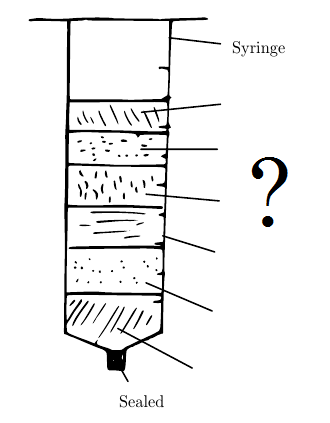
\includegraphics[width=0.3\textwidth]{./img/density-tower-sci-meth.png}
\end{center}

\begin{description*}
\item[Materials:]{Syringes, bottles, water, cooking oil, kerosene, spirit, honey, glycerine, tape, scissors}
\item[Setup:]{Prepare a test tube rack by cutting a bottle and filling it with dirt. Remove the plungers from the syringes and seal them with tape, super glue, or by melting to opening closed.}\\
\item[Problem:]{Which liquids are more dense than others?\\

\begin{tabular}{|l|c|c|} \hline
\multirow{2}{*}{\textbf{Liquid}} & \textbf{Hypothesis} & \multirow{2}{*}{\textbf{Experimental Result}} \\
& \textbf{(Position, 1 = bottom)} & \\ \hline
Water & & \\ \hline
Cooking oil & & \\ \hline
Kerosene & & \\ \hline
Spirit & & \\ \hline
Honey & & \\ \hline
Glycerine & & \\ \hline
\end{tabular} \\[10pt]
}\\
\item[Hypothesis:]{Predict the order in which the liquids will settle from the bottom of the syringe. Assign 1 to the bottom liquid, 2 to the one above it, and so on.}
\item[Procedure:]{Pour a small amount of each liquid into a syringe, observing after each addition.}
\item[Observations:]{After adding all liquids, record the order in which they rest, starting with 1 at the bottom.}
\item[Questions:]{}\hfill
\begin{enumerate}
\item Which liquid finished at the bottom?
\item Which liquid finished at the top?
\item Which liquid has the greatest density?
\item Which liquid has the lowest density?
\item What happens if you place a small object (e.g. paper clip, eraser, paper) in the tower? 
\end{enumerate}
\item[Theory:]{\emph{Density} is a property of different materials and liquids. It is a ratio of its mass to its volume. Dense liquids sink to the bottom, while less dense liquids rise to the top. A small object placed in the tower will settle in the liquid which is nearest its own density.}
\end{description*}

\pagebreak


\subsection{Sinkers and Floaters}

%\begin{center}
%\includegraphics[width=0.4\textwidth]{./img/source/.jpg}
%\end{center}

\begin{description*}
\item[Materials:]{Basin of water, various objects, e.g. nail, paper clip, paper, aluminum foil, soda cap, matchbox, pen cap, toothpick, balloons, flour}
%\item[Setup:]{}\\
\item[Problem:]{Which objects sink or float when placed in water?\\

\begin{tabular}{|l|c|c|} \hline
\multirow{2}{*}{\textbf{Object}} & \textbf{Hypothesis} & \multirow{2}{*}{\textbf{Experimental Result}} \\
& \textbf{(Sink or Float)} & \\ \hline
Nail& & \\ \hline
Paper clip& & \\ \hline
Pen cap& & \\ \hline
Soda cap (dropped)& & \\ \hline
Soda cap (placed carefully)& & \\ \hline
Toothpick & & \\ \hline
Paper& & \\ \hline
Aluminum foil& & \\ \hline
Matchbox& & \\ \hline
Balloon (empty)& & \\ \hline
Balloon (filled with flour)& & \\ \hline
Balloon (filled with water)& & \\ \hline
Balloon (filled with air)& & \\ \hline
\end{tabular} \\[10pt]
}\\
\item[Hypothesis:]{Predict whether each object will sink or float when placed in the basin of water. Record in the table.}
\item[Procedure:]{Place each object in the water. First place an object very carefully, then drop it in.}
\item[Observations:]{Record the results in the table.}
\item[Questions:]{}\hfill
\begin{enumerate}
\item What factors affect whether an object sinks or floats?
\item How do large objects such as boats float?
\end{enumerate}
\item[Theory:]{\emph{Flotation} depends on several things. A bottle cap placed carefully on the surface of the water will float, but when pushed under, will sink. A sheet of aluminum foil will float while a sheet of the same size which is folded several times will sink. A balloon filled with flour sinks, one filled with water just floats, and one filled with air floats above the surface.\\

If an object's \emph{total density} is greater than that of water, it sinks, but if less than water, it floats. Air has a density less than water, so when air is trapped in objects such as bottle caps or balloons, they float because their total density is less than water. When air is removed (folded aluminum foil) or replaced by water (bottle cap), the total density of the object is just the density of the material. A matchbox pushed under water rises back to the surface because its density is less than that of water.\\

Boats are able to float despite being built from dense materials because of the large volume of water they displace and the large amount of air inside the boat. A boat with a larger surface area displaces a larger volume of water and thus can carry a larger load before sinking.\\

Follow up this activity with the \emph{Raft Rally} science competition.}
\end{description*}

\pagebreak

\subsection{Mixing Colours}

%\begin{center}
%\includegraphics[width=0.4\textwidth]{./img/source/.jpg}
%\end{center}

\begin{description*}
\item[Materials:]{Various food colours, syringes, bottle, scissors, tape, paper}
\item[Setup:]{Prepare a test tube rack by cutting a bottle and filling it with dirt. Remove the plungers from the syringes and seal them with tape, super glue, or by melting to opening closed.}\\
\item[Problem:]{What happens when we mix different colours?\\

\begin{tabular}{|l|c|c|} \hline
\multirow{2}{*}{\textbf{Colours to Mix}} & \textbf{Hypothesis} & \multirow{2}{*}{\textbf{Experimental Result}} \\
& \textbf{(What colour?)} & \\ \hline
Red and green & & \\ \hline
Yellow and blue & & \\ \hline
Red and yellow & & \\ \hline
All colours & & \\ \hline
\end{tabular} \\[10pt]
}\\
\item[Hypothesis:]{Predict which colour will result when the two colours given are mixed together. Record it in the table.}
\item[Procedure:]{Use syringes to remove small amounts of each colour and place on a sheet of paper. Be sure to lay down plenty of paper so that the colours do not bleed through onto the table!}
\item[Observations:]{Record the resulting colour mixture in the table.}
\item[Questions:]{}\hfill
\begin{enumerate}
\item How can you make orange from other colours?
\item What colour do you get by mixing all of the colours together?
\item What are some uses of coloured dyes?
\end{enumerate}
\item[Theory:]{Red, green and blue are \emph{primary colours} of light. Other colours are made by different combinations of these primary colours. Coloured dyes are used for many applications, including clothes, paper and printing pictures.}
\end{description*}

%==================================================================================================%

\setcounter{secnumdepth}{2}

%\end{multicols}
\vfill
\pagebreak
%\section{Measurement and Density/Relative Density}

\begin{multicols}{2}

\section*{Collection of Data}


\subsection{Data on Weighing}

\begin{center}
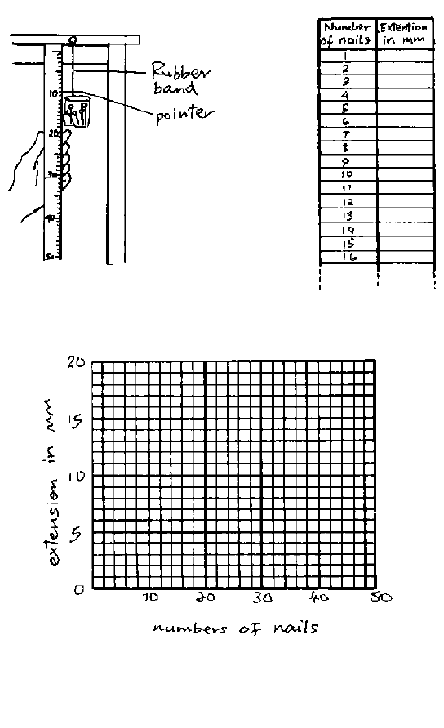
\includegraphics[width=0.4\textwidth]{./img/source/meas-mass.png}
\end{center}

Fix a rubber band at one end to a table or retort stand. At the other end, attach a paper clip to act as a pointer and a small bag or scale pan. Fill the bag or scale pan with successive numbers of nails. Have students measure the extension of the rubber band each time they add more nails. Record the readings and use the data to draw a graph as shown in the figure.

\subsection{Data on Distance}

\begin{center}
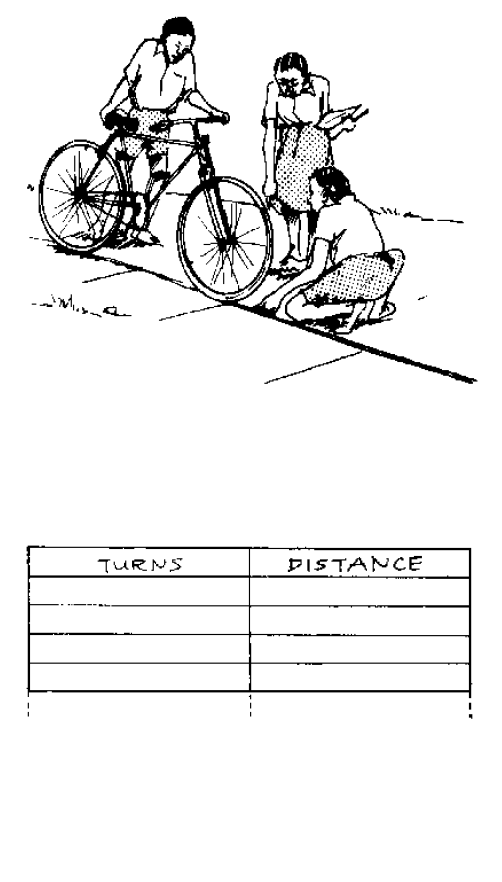
\includegraphics[width=0.4\textwidth]{./img/source/meas-distance.png}
\end{center}

Make a mark on the tyre of a bicycle at the point where it touches the ground. Turn the tyre by moving the bicycle forward and record the length of one turn. Repeat the experiment several times for various numbers of turns, each time recording the horizontal distance covered. Draw a graph to show the data.

\subsection{Data on Time}

\begin{center}
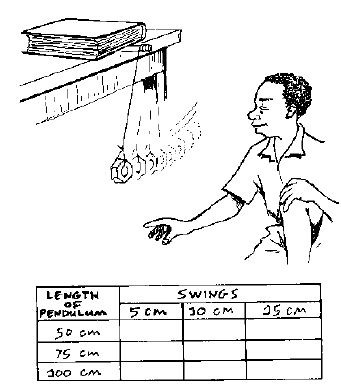
\includegraphics[width=0.4\textwidth]{./img/source/meas-time.png}
\end{center}

Fix a string just off the edge of a table and hang a small weight (e.g. a nut or nail) at a distance of 50 cm. This is a simple pendulum. Pull the pendulum to one side so that its horizontal displacement is 5 cm. Count the number of oscillations (back and forth) made in one minute. Repeat by increasing the horizontal displacement to 10 cm and 15 cm. Then try varying the length of the string. How long must the pendulum be to oscillate 60 times in one minute?

%\subsection{Mass vs. Weight}

%==================================================================================================%

\section*{Measuring Instruments}


\subsection{Construction of a Metre Rule}
\label{sub:metrerule}

\begin{description*}
%\item[Subtopic:]{Concept of Measurement}
\item[Materials:]{Wooden board, pen\slash pencil, a handsaw, ruler or tape measure}
%\item[Setup:]{}
\item[Procedure:]{Use the handsaw to cut a piece of wood 100 cm $\times$ 3.5 cm $\times$ 0.5 cm. Use a ruler or tape measure to mark a scale in cm on the wood.}
%\item[Hazards:]{}
%\item[Questions:]{}
%\item[Observations:]{}
%\item[Theory:]{}
\item[Applications:]{Students can record data on their height, dimensions of the classroom, etc.}
\item[Notes:]{Instead of a wooden block, string can be used by making knots at different intervals.}
\end{description*}

\subsection{Construction of a Beam Balance}
\label{sub:beambalance}

\begin{center}
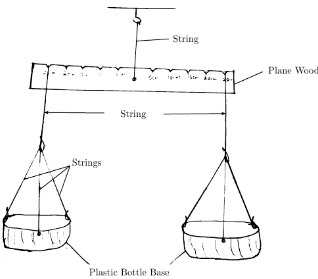
\includegraphics[width=0.4\textwidth]{./img/beam-balance.png}
\end{center}

\begin{description*}
%\item[Subtopic:]{Concept of Measurement}
\item[Materials:]{Ruler or wooden bar 30 cm $\times$ 2 cm, nails, heat source*, razor/knife, string/wire, pen, 2 \nameref{sub:scalepans}}
%\item[Setup:]{}
\item[Procedure:]{Find the balancing point of the ruler/wood block and mark it with a pen. Use a heated nail to make a hole through this point. Make notches at 5 cm intervals on either side of the center hole using a razor/knife to suspend scale pans. Use a string/wire tied through the center hole to suspend the balance.}
%\item[Hazards:]{}
%\item[Questions:]{}
%\item[Observations:]{}
%\item[Theory:]{}
\item[Applications:]{Principle of Moments}
\item[Notes:]{Use locally available \nameref{sec:masses} to find the mass of everyday objects, e.g. notebooks, pens, rulers.}
\end{description*}

\subsection{Scale Pans}
\label{sub:scalepans}

\begin{center}
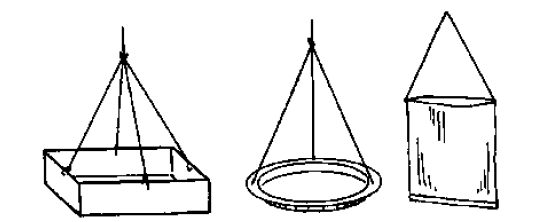
\includegraphics[width=0.4\textwidth]{./img/source/scale-pans.png}
\end{center}

\begin{description*}
%\item[Subtopic:]{Concept of Measurement}
\item[Materials:]{Match boxes, large plastic bottles, tin can lids, small plastic bags, knife, string}
%\item[Setup:]{}
\item[Procedure:]{Use a knife to poke 3~-~4 holes in the sides of one of the above materials. If using plastic bottles, cut them about 3~-~4~cm from the bottom. Cut equal lengths of string and tie them through the holes in the scale pan. Join the strings together at the upper end. }
%\item[Hazards:]{}
%\item[Questions:]{}
%\item[Observations:]{}
%\item[Theory:]{}
%\item[Applications:]{}
%\item[Notes:]{}
\end{description*}

\subsection{Construction of a Measuring Cylinder}
\label{sub:meascyl}
\begin{description*}
%\item[Subtopic:]{Concept of Measurement}
\item[Materials:]{Plastic bottles of different sizes, syringes (10 mL - 50 mL), marker pen, ruler, bucket of water}
%\item[Setup:]{}
\item[Procedure:]{Using the syringe, transfer a known volume of water from the bucket to the empty bottle. Use the marker pen to mark the level of water on the bottle. Repeat for a range of volumes, using a ruler to complete the scale.}
%\item[Hazards:]{}
%\item[Questions:]{}
%\item[Observations:]{}
%\item[Theory:]{}
%\item[Applications:]{}
%\item[Notes:]{}
\end{description*}

\subsection{Construction of a Eureka Can}
\label{sub:eurekacan}

\begin{center}
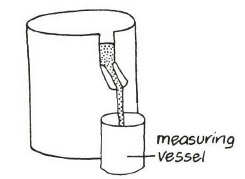
\includegraphics[width=0.2\textwidth]{./img/vso/overflow-can.png}
\end{center}

\begin{description*}
%\item[Subtopic:]{Determining the Volume of Irregular Objects}
\item[Materials:]{Plastic bottle, knife}
%\item[Setup:]{}
\item[Procedure:]{Cut a plastic bottle about 10~cm from the bottom. Cut 2 slits at the top of the bottle and bend the strip forward to form a spout.}
%\item[Hazards:]{}
%\item[Questions:]{}
%\item[Observations:]{}
%\item[Theory:]{}
\item[Applications:]{Measuring the volume of irregular objects, Archimedes' Principle}
\item[Notes:]{Alternatively, use a bottle or tin can and poke a hole near the top using a heated nail. Attach a straw/hollow pen tube/tube of aluminum foil, using super glue to ensure an air-tight seal.}
\end{description*}

\subsection{Errors in Measurement}
\label{sub:meas-errors}

\begin{description*}
%\item[Subtopic:]{}
\item[Materials:]{Metre rules, stopwatches}
%\item[Setup:]{}
\item[Procedure:]{(a) Draw a line on the board or floor. Have several students measure the length and secretly record their results. Collect the results and record them on the board, noting any differences.\\(b) Distribute stopwatches to several students. Clap twice and have students measure the time betweeen claps and secretly record their results. Collect the results and record them on the board, observing any differences.}
%\item[Hazards:]{}
\item[Questions:]{What is the best result to use for each of the collected measurements?}
%\item[Observations:]{}
\item[Theory:]{Measurements vary from person to person. Every measurement comes with some level of error, and so it is important to take care when measuring to increase accuracy. The best result to use is the average of all the measurements.}
%\item[Applications:]{}
%\item[Notes:]{}
\end{description*}

%==================================================================================================%

\section*{Density/Relative Density}

Density can be found by taking the ratio of a body's mass to its volume. Common units of density are g/mL and kg/L. $$ \mathrm{Density} = \mathrm{mass} \div \mathrm{Volume} $$$$ \rho = \cfrac{m}{V} $$
Relative density (R.D.) can be used to compare the density of a given material to that of water.  Water is the standard with a density of 1.0 g/cm$^3$ (or 1 000 kg/m$^3$), so all other densities are compared to water. Because relative density is a ratio of two densities, it has no units.
$$\mathrm{R.D.} = \frac{\mathrm{Density\; \; of \;substance}}{\mathrm{Density\; \;of \;water}}$$


%\subsection{Density of a Solid}

\subsection{Density Column}
\label{sub:density-column}

\begin{center}
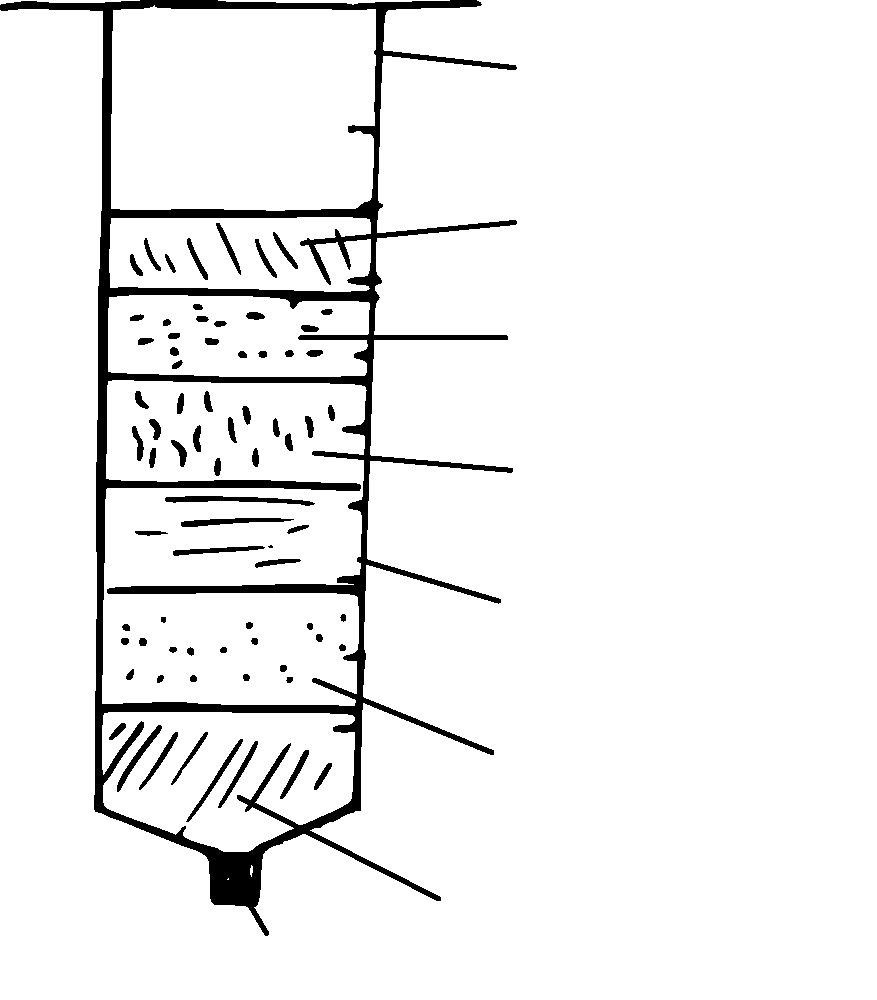
\includegraphics[width=0.25\textwidth]{./img/density-tower.png}
\end{center}

\begin{description*}
%\item[Subtopic:]{}
\item[Materials:]{Syringes, water, honey, glycerine, cooking oil, spirit, kerosene, erasers, paper clips, nails, other small objects}
%\item[Setup:]{}
\item[Procedure:]{Add each liquid into the syringe, one by one, observing the relative depths of each liquid. Place small solid objects e.g. rubber erasers, paper clips, small nails, etc. into the syringe and observe their positions relative to the various liquids.}
%\item[Hazards:]{}
\item[Questions:]{Which liquid is the most dense? Which is the least dense?}
\item[Observations:]{The denser liquids sink to the bottom while the less dense liquids rise to the top. The solid objects settle among liquids of comparable density.}
\item[Theory:]{}
\item[Applications:]{Relative densities of liquids and solids help to identify certain substances, e.g. whether a ring is really made of gold.}
\item[Notes:]{Food coloring can be added to colorless liquids such as water, kerosene and glycerine to help distinguish among them.}
\end{description*}

%\subsection{Relative Density of a Liquid}

\subsection{U-Tube Apparatus}
\label{sub:u-tube}

\begin{description*}
%\item[Subtopic:]{}
\item[Materials:]{3 clear plastic pen tubes, cardboard, heated nail or knife, tape, pen, super glue, water, kerosene.}
\item[Setup:]{Cut two of the tubes at one end to make a 45$^\circ$ angle, and cut the third tube (shorter than the other two) to make a 45$^\circ$ angle at both ends. Attach the two longer tubes to either side of the short one so that they make right angles and form a U-shape. Melt the angled ends together with a hot knife, soldering iron, etc. so that the apparatus is water-tight. Glue the assembly to a cardboard base so that it stands upright. 

Place thin strips of tape along each side of the U-tube and mark with identical scales. Do this by adding known volumes of water and marking the levels on each scale. Label these marks from top to bottom as 0, 1, 2, etc.}
\item[Procedure:]{Place an amount of water into the U-tube such that the water rises about half way on either side of the tube. The actual volume of water is not important as long as you can see the levels clearly. Stand the tube upright and slowly drip about 1 mL of kerosene into one side of the U-tube. Measure the relative heights of water and the kerosene from the bottom level of the kerosene.}
%\item[Hazards:]{}
%\item[Questions:]{}
\item[Observations:]{The kerosene will displace the water, so you should see the water level on the other side rise slightly.}
\item[Theory:]{If a fluid’s density is less than that of water, it will float on top, displacing the water on the other side of the tube. From Archimedes’ principle and the Law of Flotation, we know that \[ \frac{\text{height of water}}{\text{height of kerosene}} = \frac{\text{density of kerosene}}{\text{density of water}} \]. The scales drawn on the outside of the U-tube allow us to find the ratio of the heights without needing units, and the density of water is known to be 1.0 g/mL, so the density of the other fluid can be calculated.}
%\item[Applications:]{}
\item[Notes:]{If the other fluid has a higher density than water, the experiment can still be done, but the fluid with higher density must be added first, then displaced with water, performing the same calculation.}
\end{description*}

\end{multicols}

\pagebreak
%\section{Force}

\begin{multicols}{2}

\section*{Concept of Force}


\subsection{Examples of Forces}
\begin{center}
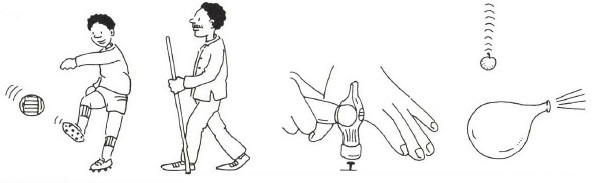
\includegraphics[width=0.5\textwidth]{./img/vso/forces-ex.jpg}
\end{center}

A \textbf{force} is any push or pull on an object. Examples of forces in our daily life include kicking a football, walking due to friction, hammering a nail and dropping an object. What other examples can you think of?

\subsection{Making a Spring Balance}

\begin{center}
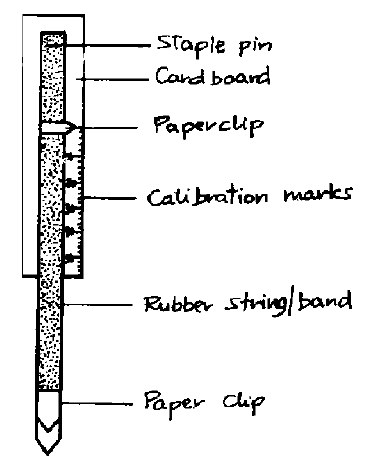
\includegraphics[width=0.26\textwidth]{./img/source/spring-balance.png}
\end{center}

\begin{description*}
%\item[Subtopic:]{Concept of Force}
%\item[Shika Rating:]{4}
\item[Materials:]{Cardboard, strong rubber band, staple pin, 2 paper clips, \nameref{sec:masses}}
\item[Setup:]{Take a strip of cardboard or wood and fix a strong rubber band to it using a staple pin. (The stronger the rubber band, the larger the force you can measure.) Attach one paper clip as a pointer as shown in the figure. Then fix another as a hook at the bottom end of the rubber band.}
\item[Procedure:]{Calibrate the balance in \emph{Newtons} using either a standard set of \nameref{sec:masses} or another spring balance. A mass of 10 g has a weight of 0.1 N; a mass of 100 g has a weight of 1 N, etc. Draw marks accordingly on the scale of the balance.}
\item[Hazards:]{Never apply such a large force that the pointer does not return to the zero mark when the force ceases.}
%\item[Questions:]{}
%\item[Theory:]{}
\item[Applications:]{Use the spring balance to measure the weight of small objects or the force of pulling an object along a table.}
%\item[Notes:]{}
\end{description*}

%==================================================================================================%

\section*{Effects of Forces}
%Forces can have a variety of effects on objects, including \emph{stretching}, \emph{compression} (or \emph{restoring}), \emph{attraction}, \emph{repulsion}, \emph{torsion}, \emph{friction}, \emph{viscosity} and \emph{air resistance}. These effects are seen all around us in our daily lives.


\subsection{Observing Effects of Forces}

\begin{center}
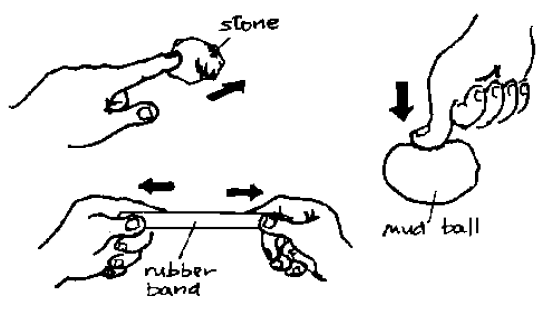
\includegraphics[width=0.45\textwidth]{./img/source/effects-forces.png}
\end{center}

\begin{description*}
%\item[Subtopic:]{}
\item[Materials:]{Rubber bands, springs, magnets, ruler, honey, water, paper}
%\item[Setup:]{}
\item[Procedure:]{Have students investigate different effects of forces using common materials.}
%\item[Hazards:]{}
%\item[Questions:]{}
\item[Observations:]{Rubber bands and springs stretch when pulled and then restore their shape. Magnets attract and repel each other. A ruler can be twisted under torsion. Rubbing hands together produces heat from friction. Honey pours more slowly than water due to a higher viscosity. A sheet of paper falls to the ground slowly because of air resistance.}
%\item[Theory:]{}
\item[Applications:]{Brainstorm various applications of the effects of forces with the class.}
%\item[Notes:]{}
\end{description*}

\subsection{Presence of Gravity}
\begin{description*}
%\item[Subtopic:]{}
\item[Materials:]{Pen, ruler, sheet of paper, book (same size as paper)}
%\item[Setup:]{}
\item[Procedure:]{Drop the pen and ruler side by side from shoulder height. Repeat with a pen and sheet of paper. Then place the paper on top of a book and drop side by side with a regular sheet of paper. Bunch the paper into a tight ball and drop it again with the book.}
%\item[Hazards:]{}
\item[Questions:]{Which objects fell at the same rate? Which ones fell more slowly?}
\item[Observations:]{All objects, with the exception of paper and other light, wide objects, fall at exactly the same rate.}
\item[Theory:]{Gravity pulls on all objects on earth the same.  The paper falls slowly because it is more affected by air resistance due to its small weight and large surface area. Placing a book under the paper reduces air resistance by blocking all of the air which would normally push against the paper. Thus they fall at the same rate.  When the paper is bunched into a ball, the mass stays the same but the air resistance is greatly reduced so it falls at the same rate as the book.}
%\item[Applications:]{}
%\item[Notes:]{}
\end{description*}

\subsection{Helicopters}

\begin{center}
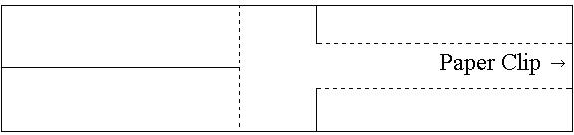
\includegraphics[width=0.4\textwidth]{./img/helicopter-1.png}
\end{center}

\begin{center}
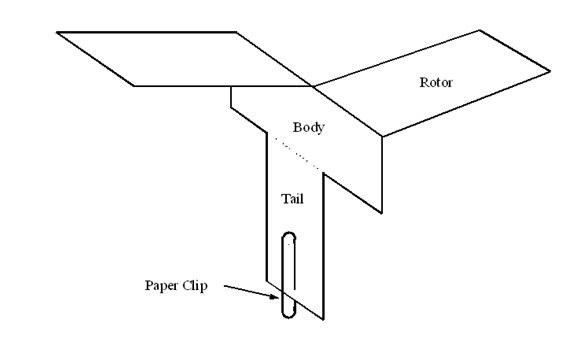
\includegraphics[width=0.4\textwidth]{./img/helicopter-2.png}
\end{center}

\begin{description*}
%\item[Subtopic:]{}
\item[Materials:]{Paper, scissors, paper clip}
%\item[Setup:]{}
\item[Procedure:]{Copy the following design onto a piece of paper. Cut along the solid lines and fold along the dotted lines, attaching the paper clip to the bottom. Drop the helicopter with the paperclip down and watch it spin!}
%\item[Hazards:]{}
\item[Questions:]{Does the helicopter spin more if you add more paper clips? If you change the size/number of wings?}
\item[Observations:]{Adding more paper clips causes the helicopter to spin faster. Increasing the surface area of the wings also increases the rate of spin.}
\item[Theory:]{The helicopter spins because the force of air resistance pushing up on the wings creates a moment about the vertical axis of rotation. Increasing the force of air resistance increases this moment and the helicopter spins faster.}
%\item[Applications:]{}
%\item[Notes:]{}
\end{description*}

\subsection{Forces on Bridges}

\begin{center}
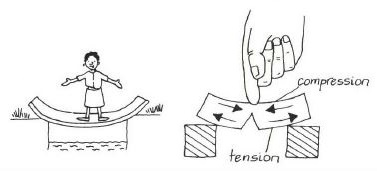
\includegraphics[width=0.5\textwidth]{./img/vso/forces-bridges.jpg}
\end{center}

\begin{description*}
%\item[Subtopic:]{}
%\item[Materials:]{}
%\item[Setup:]{}
%\item[Procedure:]{}
%\item[Hazards:]{}
%\item[Questions:]{}
%\item[Observations:]{}
\item[Theory:]{The bridge bends under the
weight of the load. More than
one force is at work. Compression
forces are concentrated on the
top surface. When a bridge
bends, compression on top
creates tension forces on the
bottom surface.}
%\item[Applications:]{}
%\item[Notes:]{}
\end{description*}

\subsection{Parachutes}

\begin{center}
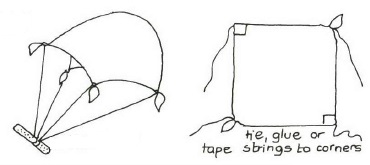
\includegraphics[width=0.4\textwidth]{./img/vso/parachute.jpg}
\end{center}

\begin{description*}
%\item[Subtopic:]{}
\item[Materials:]{Paper/newspaper/plastic bags, string, paper clips}
\item[Setup:]{Tie pieces of string (about 30 cm) to each corner of the paper/bag. Join the four strings together and attach a paper clip or other small weight.}
\item[Procedure:]{Drop the parachute side by side with a normal paper clip.}
%\item[Hazards:]{}
\item[Questions:]{Which one reaches the ground first? If the paper clip were a person, which one would arrive safely to the ground? Does a person using a parachute want to make it as large as possible or as small as possible?}
\item[Observations:]{The parachute falls more slowly because there is a larger space for air to enter and counteract the force of gravity pulling it to the ground.}
%\item[Theory:]{}
\item[Applications:]{Skydivers, military personnel, air-dropped aid packages. Follow up this activity with the \emph{Egg Drop} or \emph{Drop Zone} science competitions (see \emph{Shika na Mikono} resource manual).}
%\nameref{sec:drop-zone} or \nameref{sec:egg-drop} science competitions (p.~\pageref{ec:egg-drop}).}
\item[Notes:]{Poke a small hole in the top of the parachute and ask students what will happen.}
\end{description*}

\subsection{Strengthening Bridges}

\begin{center}
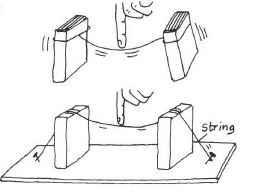
\includegraphics[width=0.4\textwidth]{./img/vso/strengthening-bridges.jpg}
\end{center}

\begin{description*}
%\item[Subtopic:]{}
\item[Materials:]{Books, string, nails, board}
%\item[Setup:]{}
\item[Procedure:]{Ask students to build the 2
bridges shown. Discuss why the
suspension bridge is stronger.}
%\item[Hazards:]{}
%\item[Questions:]{}
%\item[Observations:]{}
\item[Theory:]{In a suspension bridge the tension
in the bridge is increased by
securing the `strings' and
suspending them over towers or
from trees.}
\item[Applications:]{Follow up the discussion by having students compete in the \emph{Bridge Challenge} science competition (see \emph{Shika na Mikono} resource manual).}
%\nameref{sec:bridge-challenge} science competition (p.~\pageref{sec:bridge-challenge}).}
%\item[Notes:]{}
\end{description*}


\end{multicols}

\pagebreak
%\section{Archimedes' Principle and the Law of Flotation}

\begin{multicols}{2}


\section*{Concept of Upthrust}
\textbf{Archimedes' Principle} states that any object partially or totally immersed in a fluid experiences an upthrust equal to the weight of the fluid displaced by the body.
$$ \text{Upthrust} = \text{Weight of displaced fluid}$$
%$$ \text{Weight in air} - \text{Apparent weight in fluid} = \text{Weight of displaced fluid}$$

\subsection{Verifying Archimedes' Principle}

\begin{center}
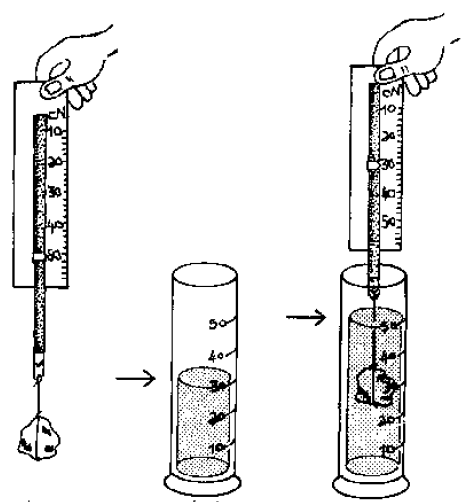
\includegraphics[width=0.4\textwidth]{./img/source/upthrust.png}
\end{center}

\begin{description*}
%\item[Subtopic:]{}
\item[Materials:]{\nameref{sec:spring-balance}, stone, string, \nameref{sec:meascyl}, water, \nameref{sec:eureka-can}, syringe}
%\item[Setup:]{}
\item[Procedure:]{Tie a string around a stone and measure its weight in Newtons using a spring balance. Fill the measuring cylinder partially with water and record the reading. Immerse the stone fully into the water (without touching the bottom) and record the reading on the spring balance, as well as the new water level of the measuring cylinder.}
%\item[Hazards:]{}
\item[Questions:]{What is the change in weight of the stone as read from the spring balance? What is the weight of the displaced water (1 mL = 0.01 N)?}
%\item[Observations:]{}
\item[Theory:]{The change in weight of the stone is known as its \emph{Apparent Loss in Weight}, which is equal to the \emph{Upthrust} exerted on the stone by the water. Archimedes' Principle tells us that this is equal to the weight of the water displaced by the stone.}
%\item[Applications:]{}
\item[Notes:]{A Eureka can and syringe may be used to measure the displaced fluid in place of a measuring cylinder.}
\end{description*}

%==================================================================================================%

\section*{Sinking and Floating}
If the density of an object is less than that of the surrounding fluid, the object will float. If the density is greater than that of the fluid, it will sink.

\textbf{The Law of Flotation} states that a floating body displaces its own weight of the fluid in which it floats.
$$\text{Weight of body} = \text{Weight of displaced fluid}$$


\subsection{Verifying the Law of Flotation}

\begin{center}
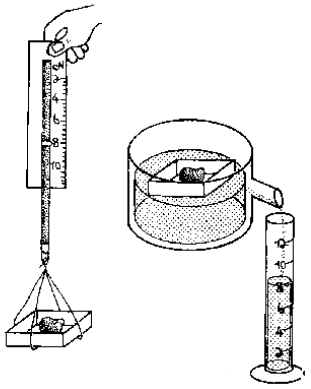
\includegraphics[width=0.4\textwidth]{./img/source/flotation.png}
\end{center}

\begin{description*}
%\item[Subtopic:]{}
\item[Materials:]{\nameref{sec:spring-balance}, matchbox, stone, string, \nameref{sec:eureka-can}, \nameref{sec:meascyl}/syringe}
%\item[Setup:]{}
\item[Procedure:]{Load a matchbox with a small stone so that it still floats in water. Record the weight of the matchbox and stone in Newtons using a spring balance. Fill the Eureka can with water and allow the matchbox to float on it. Collect the overflow in a measuring cylinder or syringe. Calculate the weight of the overflow (1 mL = 0.01 N).}
%\item[Hazards:]{}
\item[Questions:]{How does the weight of the matchbox and stone compare to that of the displaced water?}
\item[Observations:]{The values should be equal, thus verifying the Law of Flotation.}
%\item[Theory:]{}
\item[Applications:]{Submarine, hot air balloon, ships. Design and selection of materials for these vessels are done using the Law of Flotation.}
%\item[Notes:]{}
\end{description*}

\vfill
\columnbreak

\subsection{Sinkers and Floaters}

%\begin{center}
%\includegraphics[width=0.4\textwidth]{./img/.jpg}
%\end{center}

\begin{description*}
%\item[Subtopic:]{}
\item[Materials:]{Basin of water, various objects, e.g. nail, paper clip, paper, aluminum foil, soda cap, matchbox, pen cap, toothpick, balloons, flour}
\item[Setup:]{Fill one balloon with flour, one with water, and one with air. They should all be the same size.}
\item[Procedure:]{Have students predict the outcome for each object. Then place each object in the water, first by placing very carefully, then by dropping it in.}
\end{description*}

\begin{tabular}{|l|c|} \hline
\textbf{Object} & \textbf{Sink or Float?} \\ \hline
Nail&  \\ \hline
Paper clip&  \\ \hline
Pen cap&  \\ \hline
Soda cap &  \\ \hline
Toothpick &  \\ \hline
Paper&  \\ \hline
Aluminum foil&  \\ \hline
Matchbox&  \\ \hline
Balloon (empty)&  \\ \hline
Balloon (flour)&  \\ \hline
Balloon (water)&  \\ \hline
Balloon (air)&  \\ \hline
\end{tabular} \\[10pt]
%\item[Hazards:]{}
\begin{description*}
\item[Questions:]{}\hfill
\begin{enumerate}
\item What factors affect whether an object sinks or floats?
\item How do large objects such as boats float?
\end{enumerate}
\item[Observations:]{A bottle cap placed carefully on the surface of the water will float, but when pushed under, will sink. A sheet of aluminum foil will float while a sheet of the same size which is folded several times will sink. A balloon filled with flour sinks, one filled with water just floats, and one filled with air floats above the surface.}
\item[Theory:]{If an object's \emph{total density} is greater than that of water, it sinks, but if less than water, it floats. Air has a density less than water, so when air is trapped in objects such as bottle caps or balloons, they float because their total density is less than water. When air is removed (folded aluminum foil) or replaced by water (bottle cap), the total density of the object is just the density of the material. A matchbox pushed under water rises back to the surface because its density is less than that of water.

%Boats are able to float despite being built from dense materials because of the large volume of water they displace and the large amount of air inside the boat. A boat with a larger surface area displaces a larger volume of water and thus can carry a larger load before sinking.
}
\item[Applications:]{See the section on \nameref{sec:scientific-method} (p.~\pageref{sec:scientific-method}) to conduct this activity as an experiment with students. Follow up this activity with the \emph{Raft Rally} science competition (see \emph{Shika na Mikono} resource manual).}
%\item[Notes:]{}
\end{description*}

\subsection{Egg Float}

\begin{center}
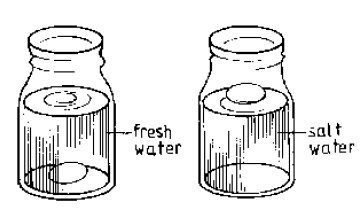
\includegraphics[width=0.49\textwidth]{./img/source/egg-float.png}
\end{center}

\begin{description*}
%\item[Subtopic:]{}
\item[Materials:]{2 fresh eggs, 2 containers (bottles cut in half), salt (less than half a cup)}
\item[Setup:]{Fill the two containers with water and place a fresh egg in each.}
\item[Procedure:]{Leave one as it is and add salt to the other. Add and mix salt until the egg floats in the saltwater container.}
%\item[Hazards:]{}
\item[Questions:]{Why does the egg float in saltwater but sink in fresh water?}
%\item[Observations:]{}
\item[Theory:]{Saltwater has a greater density than fresh water. A fresh egg has a density between fresh water and saltwater. Since an egg is denser than freshwater, it sinks. Since an egg is less dense than saltwater, it floats.}
\item[Applications:]{This is the same reason why it is easier to stay afloat when swimming in the ocean (saltwater) as opposed to a lake (fresh water).}
%\item[Notes:]{}
\end{description*}

\subsection{Floating Candle}

\begin{center}
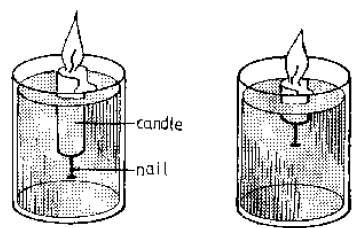
\includegraphics[width=0.45\textwidth]{./img/source/floating-candle.png}
\end{center}

\begin{description*}
%\item[Subtopic:]{}
\item[Materials:]{Candle, nail, container, water}
%\item[Setup:]{}
\item[Procedure:]{Put a nail into the bottom end of a candle so that the candle just floats with its top a bit above the surface of the water. Light the candle and watch as it burns up.}
%\item[Hazards:]{}
\item[Questions:]{Why does the candle continue to float even though it loses weight as it burns up?}
%\item[Observations:]{}
\item[Theory:]{The candle continues to float because its density remains less than that of the surrounding water.}
%\item[Applications:]{}
%\item[Notes:]{}
\end{description*}

\vfill

\subsection{Cartesian Diver}

\begin{center}
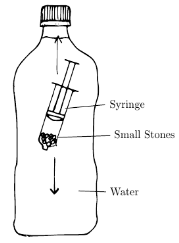
\includegraphics[width=0.3\textwidth]{./img/cartesian-diver.png}
\end{center}

\begin{description*}
%\item[Subtopic:]{}
\item[Materials:]{1.5 L plastic bottle, balloon, paper clips (large), water}
\item[Setup:]{Fill the bottle with water. Fix a large paper clip to the lip of a balloon. Making sure to keep all air out of the balloon, insert it into the bottle. It should just float at the top while remaining completely submerged. Adjust depending on type of balloon and paper clips.}
\item[Procedure:]{Screw the cap on the bottle and squeeze the middle of the bottle, then release.}
%\item[Hazards:]{}
%\item[Questions:]{}
\item[Observations:]{The balloon should begin to sink when you squeeze, but float again when you release.}
\item[Theory:]{While water is nearly incompressible, the balloon (and any small amount of air inside) is compressible. This means when you squeeze the bottle, the water remains unchanged, but the balloon is compressed, decreasing its volume and so increasing its density. Before squeezing, it was less dense than the water and so it floated. After squeezing, it becomes denser than the water and sinks.}
%\item[Applications:]{}
%\item[Notes:]{}
\end{description*}

\subsection{The Hydrometer}

\begin{center}
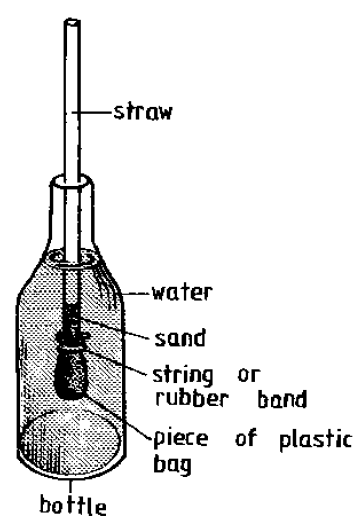
\includegraphics[width=0.35\textwidth]{./img/source/hydrometer.png}
\end{center}

\begin{description*}
%\item[Subtopic:]{}
\item[Materials:]{Bottle, straw, plastic bag, dry sand, rubber band/string, pen, ruler, water, kerosene, other liquids}
\item[Setup:]{Close one end of the straw with the plastic bag and secure it with the rubber band so that water cannot enter. Pour sand into the straw until it floats upright in the bottle of water without touching the bottom or leaning.}
\item[Procedure:]{Use a pen to mark the water level on the outside of the straw. Label it 1.0 (the density of water in g/cm$^3$). Place the straw upright in a container of kerosene. Mark the kerosene level on the straw as 0.8 (known density of kerosene). Remove and clean the straw, without getting any liquid inside. Use a ruler to complete the scale above 1.0 and below 0.8, beginning with 0.9 at the midpoint. Use the hydrometer to measure the densities of other liquids.}
%\item[Hazards:]{}
\item[Questions:]{Why do smaller numbers appear at the top of the hydrometer scale?}
%\item[Observations:]{}
\item[Theory:]{Liquids with a lower density allow the hydrometer to sink deeper, and thus the liquid reaches a higher point on the scale.}
%\item[Applications:]{}
%\item[Notes:]{}
\end{description*}


\end{multicols}

\pagebreak
%\section{Structure and Properties of Matter}

\begin{multicols}{2}

\section*{States of Matter}
All matter is made up of particles. These particles are in constant motion which increases with their temperature. Depending on temperature, matter may exist in three states: \emph{solid}, \emph{liquid} or \emph{gas}.


\subsection{Student Particles}

\begin{center}
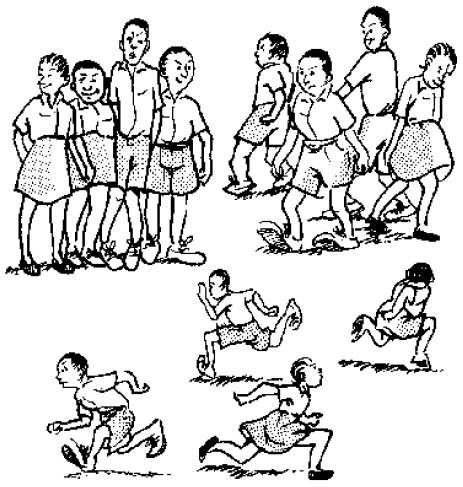
\includegraphics[width=0.4\textwidth]{./img/source/states-matter.png}
%\includegraphics[width=0.4\textwidth]{./img/vso/states-matter.png}
\end{center}

\begin{description*}
%\item[Subtopic:]{}
%\item[Materials:]{}
%\item[Setup:]{}
\item[Procedure:]{Use students to demonstrate the concept of states of matter.}
%\item[Hazards:]{}
%\item[Questions:]{}
%\item[Observations:]{}
\item[Theory:]{When students or objects are close together, they represent particles in the \emph{solid} state. As they move apart and past each other they represent particles in the \emph{liquid} state. Fast and randomly moving pupils or objects represent particles in the \emph{gaseous} state.}
%\item[Applications:]{}
%\item[Notes:]{}
\end{description*}

\subsection{A Model of Motion}

\begin{center}
\includegraphics[width=0.49\textwidth]{./img/vso/motion-model.png}
\end{center}

\begin{description*}
%\item[Subtopic:]{}
%\item[Materials:]{}
%\item[Setup:]{}
\item[Procedure:]{Put some dry beans, rice or stones in a clear bottle. Hold the bottle still, then turn it, then shake it vigorously.}
%\item[Hazards:]{}
\item[Questions:]{Which activity corresponds to which state of matter?}
%\item[Observations:]{}
\item[Theory:]{The movement of particles in solids is small and hence they are in fixed order. In liquids the particles move past each other and have lost the stiff order. In gases they move very fast and randomly, losing all order.}
%\item[Applications:]{}
%\item[Notes:]{}
\end{description*}

\subsection{Changes of State}

\begin{center}
\includegraphics[width=0.25\textwidth]{./img/source/change-state.png}
\end{center}

\begin{description*}
%\item[Subtopic:]{}
\item[Materials:]{Tin can, glass bottle, water, \nameref{sec:heatsources}*}
%\item[Setup:]{}
\item[Procedure:]{Pour a small amount of water into a tin can and heat it until it boils. Fill a bottle with cool water and hold it above the tin can.}
%\item[Hazards:]{}
%\item[Questions:]{}
\item[Observations:]{Water drops form on the outside of the cool bottle when it is touched by the steam of the boiling water.}
\item[Theory:]{Water particles escape from the boiling water as vapour and condense on the lower surface of the bottle to form water droplets. This is indirect evidence that water is made up of small particles.}
%\item[Applications:]{}
%\item[Notes:]{}
\end{description*}

%==================================================================================================%

\section*{Particulate Nature of Matter}


\subsection{Salt is Made of Particles}

\begin{center}
\includegraphics[width=0.4\textwidth]{./img/source/salt-particles.png}
\end{center}

\begin{description*}
%\item[Subtopic:]{}
\item[Materials:]{Salt/sugar, cup, water}
%\item[Setup:]{}
\item[Procedure:]{Roll some salt or sugar crystals between your fingers to feel their hardness. Taste the crystals. Take a sip of the water. Now put the salt or sugar crystals in the water and shake it. Taste again.}
%\item[Hazards:]{}
%\item[Questions:]{}
\item[Observations:]{The crystals are hard and of cubical shape. They dissolve in water and the solution tastes like salt or sugar.}
\item[Theory:]{Sugar and salt are made up of tiny particles that can be identified by tasting even though they can not be seen as a solution.}
%\item[Applications:]{}
%\item[Notes:]{}
\end{description*}

\subsection{Weighing Particles}

\begin{center}
\includegraphics[width=0.4\textwidth]{./img/source/weighing-particles.png}
\end{center}

\begin{description*}
%\item[Subtopic:]{}
\item[Materials:]{\nameref{sub:beambalance}*, small pieces of wood, \nameref{sec:heatsources}}
%\item[Setup:]{}
\item[Procedure:]{Weight pieces of wood and record the weight. Then burn the wood and weigh the ash.}
%\item[Hazards:]{}
\item[Questions:]{Is there a difference between the two weights?}
%\item[Observations:]{}
\item[Theory:]{The weight of the ash is less than that of wood. The loss in weight is due to particles which escaped as soot and gas.}
\item[Applications:]{This is why garbage reduces in size when burned. Burning wood and garbage releases carbon dioxide and other harmful gases into our environment. This is one form of \emph{pollution}.}
%\item[Notes:]{}
\end{description*}

%==================================================================================================%

\section*{Elasticity}


\subsection{Hooke's Law}
\textbf{*NECTA PRACTICAL*}
\begin{center}
\includegraphics[width=0.49\textwidth]{./img/source/elasticity.png}
\end{center}

\begin{description*}
%\item[Subtopic:]{}
\item[Materials:]{Rubber band/elastic strip, ruler, staple pin, \nameref{sec:retort-stand}*, \nameref{sub:scalepans}*, nails/small \nameref{sec:masses}*}
\item[Setup:]{Fix a rubber band at one end to a table or retort stand. At the other end, attach a paper clip to act as a pointer and a small bag or scale pan.}
\item[Procedure:]{Fill the scale pan with successive numbers of nails or known weights. Have students measure the extension of the rubber band each time they add more weights. Record the readings and use the data to draw a graph of force (weight) against extension.}
%\item[Hazards:]{}
\item[Questions:]{What is the relationship between number of weights added and extension of the rubber band? What does the slope of the graph represent?}
%\item[Observations:]{}
\item[Theory:]{Hooke's Law states that the force applied to an elastic object is directly proportional to its extension ($F = kx$). Graphing the applied \emph{weight} (in Newtons) against the extension (in metres), the slope represents the spring constant of the elastic material in N/m. }
%\item[Applications:]{}
%\item[Notes:]{}
\end{description*}

%==================================================================================================%

\section*{Adhesion and Cohesion}
Forces between particles of the same material are called \emph{cohesive forces} while those between particles of different materials are called \emph{adhesive forces}.


\subsection{Exploring Adhesion and Cohesion}

\begin{center}
\includegraphics[width=0.4\textwidth]{./img/adhesion-cohesion.png}
\end{center}

\begin{description*}
%\item[Subtopic:]{}
\item[Materials:]{Sheet of glass, water, honey, glycerin, cooking oil, syringe, and 2 wooden blocks}
%\item[Setup:]{}
\item[Procedure:]{Place a sheet of glass over two wooden blocks on a table. Using a syringe, place a drop of different liquids on the glass.}
%\item[Hazards:]{}
%\item[Questions:]{}
\item[Observations:]{Water spreads and wets the glass, while honey, glycerin and cooking oil remain in a spherical shape.}
\item[Theory:]{The adhesive forces between the water molecules and glass molecules are greater, while the cohesive forces between the molecules of honey, glycerin and cooking oil are larger.}
%\item[Applications:]{}
%\item[Notes:]{}
\end{description*}

\subsection{Pinching Water}
\begin{description*}
%\item[Subtopic:]{}
\item[Materials:]{500 mL water bottle, needle/pin/small nail}
\item[Setup:]{Make 5 small holes at the bottom of the bottle with a syringe needle or nail. Make them close together (about 5 mm apart).}
\item[Procedure:]{Fill the bottle with water and allow it to flow through the holes at the bottom. Use your thumb and forefinger to pinch the streams together to form a single stream. Pass your hand in front of the holes and all five will appear again.}
%\item[Hazards:]{}
%\item[Questions:]{}
%\item[Observations:]{}
\item[Theory:]{Water has a tendency to cling to itself due to its surface tension and cohesion. As you bring the streams together, you allow the water to stick to itself forming a single stream. Passing your hand in front again stops the flow of water at the holes and allows it to start again, which it will do in five streams.}
%\item[Applications:]{}
%\item[Notes:]{}
\end{description*}

\subsection{Water Drops}

\begin{center}
\includegraphics[width=0.3\textwidth]{./img/source/water-drops.png}
\end{center}

\begin{description*}
%\item[Subtopic:]{}
\item[Materials:]{Syringe or water dropper}
%\item[Setup:]{}
\item[Procedure:]{Slowly drip water from the syringe or water dropper. Observe how the drop forms.}
%\item[Hazards:]{}
%\item[Questions:]{}
\item[Observations:]{The water stream grows thinner and thinner as it moves further down and finally breaks to form drops.}
\item[Theory:]{Strong cohesive forces hold the water molecules together, until they are overcome by gravity and the water breaks off as drops.}
%\item[Applications:]{}
%\item[Notes:]{}
\end{description*}

%==================================================================================================%

\section*{Surface Tension}


\subsection{Pin Float}

\begin{center}
\includegraphics[width=0.49\textwidth]{./img/source/pin-float.png}
\end{center}

\begin{description*}
%\item[Subtopic:]{}
\item[Materials:]{Cup or small dish, straight pin/razor/paper clip, water, detergent}
%\item[Setup:]{}
\item[Procedure:]{Fill the cup with clean water and carefully float a pin, razor or small paper clip. Now add a small amount of detergent to the water and observe what happens.}
%\item[Hazards:]{}
%\item[Questions:]{}
\item[Observations:]{The objects float on the surface of the water initially, but after adding detergent, they sink to the bottom.}
\item[Theory:]{The surface tension of the water acts as an elastic membrane and is strong enough to support the small objects. Soap lowers the surface tension of water and therefore the objects sink.}
%\item[Applications:]{}
%\item[Notes:]{}
\end{description*}

\subsection{Water Dome}

\begin{center}
\includegraphics[width=0.2\textwidth]{./img/source/water-dome.png}
\end{center}

\begin{description*}
%\item[Subtopic:]{}
\item[Materials:]{Coin, water, syringe or eyedropper}
%\item[Setup:]{}
\item[Procedure:]{Place the coin flat on a table. Use the syringe or eyedropper to carefully drop individual water drops onto the coin.}
%\item[Hazards:]{}
\item[Questions:]{How many drops do you think the coin can hold?}
\item[Observations:]{The coin holds a surprising number of drops and forms a dome shape before the water spills over.}
\item[Theory:]{The surface tension of the water holds it together against the force of gravity, which is trying to pull the water off the coin.}
%\item[Applications:]{}
%\item[Notes:]{}
\end{description*}

\subsection{Blowing Bubbles}
\begin{description*}
%\item[Subtopic:]{}
\item[Materials:]{Thin piece of wire (approximately 30cm), water, detergent, glycerin (optional)}
\item[Setup:]{Bend the wire to form a loop of 2 to 3 cm in diameter, circling this loop many times. Leave a straight piece several cm long as a handle. Make a concentrated solution of detergent in water with a small amount of glycerin.}
\item[Procedure:]{Dip the circular part of the wire into the detergent. You should see a thin soapy film across the circle upon removal. Gently blow through the circle until a bubble separates from the wire.}
%\item[Hazards:]{}
%\item[Questions:]{}
\item[Observations:]{While blowing, the solution is being pulled back towards the surface. Once it breaks free as a bubble, it forms a spherical shape.}
\item[Theory:]{The surface tension of water causes the bubble to form the shape with the minimum surface area, which is a sphere.}
%\item[Applications:]{}
%\item[Notes:]{}
\end{description*}

%==================================================================================================%

\section*{Capillarity}

\subsection{Capillary Rise}
\begin{description*}
%\item[Subtopic:]{}
\item[Materials:]{Clear thin plastic straws with different diameters, shallow container (bottom of a water bottle/jar cap), various liquids, e.g. water, spirit and cooking oil}
%\item[Setup:]{}
\item[Procedure:]{Place one end of a straw into a container of water 1 cm deep so that the end is submerged but not touching the bottom. Mark the change in water level in the straw after about a minute. Repeat for different liquids and different size straws.}
%\item[Hazards:]{}
\item[Questions:]{Which liquid rises the farthest up the straw? Do liquids rise faster in wide or thin straws?}
\item[Observations:]{The spirit rises to the greatest height while water rises the least. Liquids rise faster in thin straws compared to thick ones.}
\item[Theory:]{Capillary rise results from adhesion, allowing the liquid to climb along the surface of the tube, as well as cohesion, which pulls the remainder of the liquid up. In a thin container, a larger proportion of liquid is attached to the side of the tube and a smaller proportion is being held by surface tension, so the adhesive force is strong enough to pull all the liquid up the tube.}
%\item[Applications:]{}
%\item[Notes:]{}
\end{description*}

\subsection{Moving Matches}

%\begin{center}
%\includegraphics[width=0.4\textwidth]{./img/.png}
%\end{center}

\begin{description*}
%\item[Subtopic:]{}
\item[Materials:]{Matches, water, straw, plastic lid}
%\item[Setup:]{}
\item[Procedure:]{Break several matches near the middle, but not so that they come apart. They should make acute angles. Place them on the plastic lid and place a few drops of water on the broken joints of the matches using the straw.}
%\item[Hazards:]{}
%\item[Questions:]{}
\item[Observations:]{The matches close and return to their original straight shape.}
\item[Theory:]{Water gets absorbed in the wooden matchstick and causes it to expand.}
\item[Applications:]{This is why it is difficult to open a wooden door after it rains. The water rises up the wood causing it to expand into its frame.}
%\item[Notes:]{}
\end{description*}

\subsection{Automatic Irrigation}

\begin{center}
\includegraphics[width=0.3\textwidth]{./img/source/irrigation.png}
\end{center}

Capillary action can be used to provide automatic irrigation for plants. Students can perform irrigation by dipping a porous material such as paper or cotton cloth in water.

%==================================================================================================%

\section*{Diffusion}

\subsection{Diffusion in Liquids}

\begin{center}
\includegraphics[width=0.4\textwidth]{./img/vso/diffusion.png}
\end{center}

\begin{description*}
%\item[Subtopic:]{}
\item[Materials:]{Plastic water bottle, food colour (liquid or powder)}
%\item[Setup:]{}
\item[Procedure:]{Put a drop or small amount of powdered food colour into the water without shaking and observe what happens.}
%\item[Hazards:]{}
%\item[Questions:]{}
\item[Observations:]{The colour gradually spreads throughout the water.}
\item[Theory:]{This spreading is due to the motion of the particles of food colour. This process is called \emph{diffusion}.}
\item[Applications:]{Organisms utilize diffusion to balance nutrient concentrations in cells and to transfer oxygen into the bloodstream during respiration.}
%\item[Notes:]{}
\end{description*}

\subsection{Smelling Particles}

\begin{description*}
%\item[Subtopic:]{}
\item[Materials:]{Orange or other citrus fruit, box}
%\item[Setup:]{}
\item[Procedure:]{Peel and orange and have students raise their hands when they begin to smell it. Now place a box in front of the orange and repeat the test.}
%\item[Hazards:]{}
%\item[Questions:]{}
\item[Observations:]{Students in the front center of the room should be the first to raise their hands, followed by those near the sides and in the back. When the orange is peeled behind the box it takes longer for the smell to reach the students.}
\item[Theory:]{Tiny particles from the orange peel spread by diffusion to students' noses. The box hinders the motion of the particles and so they reach the students more slowly.}
\item[Applications:]{Air fresheners and other sprays}
%\item[Notes:]{}
\end{description*}

%==================================================================================================%

\section*{Osmosis}


\subsection{Vanilla Balloon}

\begin{center}
\includegraphics[width=0.3\textwidth]{./img/vso/osmosis-vanilla.png}
\end{center}

\begin{description*}
%\item[Subtopic:]{}
\item[Materials:]{Balloon/plastic bag, vanilla, straw/syringe}
%\item[Setup:]{}
\item[Procedure:]{Place a few drops of vanilla in a deflated balloon. Now blow up the balloon and tie it shut.}
%\item[Hazards:]{}
%\item[Questions:]{}
\item[Observations:]{You can smell the vanilla through the surface of the balloon.}
\item[Theory:]{The balloon acts as a \emph{semi-permeable membrane} which allows some of the vanilla particles to pass through and reach your nose. Other particles remain inside the balloon.}
%\item[Applications:]{}
%\item[Notes:]{}
\end{description*}

\subsection{Semi-Permeable Membranes}

\begin{center}
\includegraphics[width=0.4\textwidth]{./img/vso/membrane.png}
\end{center}

\begin{description*}
%\item[Subtopic:]{}
\item[Materials:]{Glass jar, clear plastic bag, small beads or stones, beans, netting, string/rubber band}
\item[Setup:]{Place the mixture of beads and beans in the jar. Place the net and plastic bag over the top and tie them on securely.}
\item[Procedure:]{Shake the apparatus for a few seconds.}
%\item[Hazards:]{}
%\item[Questions:]{}
\item[Observations:]{Only the small beads pass through the netting. The beans remain in the jar.}
\item[Theory:]{The beads represent small molecules and the net is a semi-permeable membrane. The beans are too large to pass through and hence remain in the jar.}
\item[Applications:]{Water filters, organism cell membranes}
%\item[Notes:]{}
\end{description*}


\subsection{Potato Osmosis}

\begin{center}
\includegraphics[width=0.49\textwidth]{./img/vso/osmosis-potato-full.png}
\end{center}

\begin{description*}
%\item[Subtopic:]{}
\item[Materials:]{Potato, 2 water bottles, salt, water}
\item[Setup:]{Cut two equal size pieces of potato. Fill one bottle with fresh water and the other with a salt water solution.}
\item[Procedure:]{Put one piece of potato in each bottle. Observe over the next few hours.}
%\item[Hazards:]{}
%\item[Questions:]{}
\item[Observations:]{The potato in fresh water swells while the potato in salt water shrivels up.}
\item[Theory:]{Through osmosis, water moves from a region of low concentration to one of high concentration through a semi-permeable membrane (the potato). In fresh water, the potato has the higher salt concentration, so water enters in order to make a balance. In salt water, the concentration of the surrounding water is higher than that of the potato, so water inside the potato moves outside to dilute the salt solution.}
%\item[Applications:]{}
\item[Notes:]{Try this experiment again with a boiled potato. Do you observe any differences?}
\end{description*}


\end{multicols}

\pagebreak
%\section{Pressure}
\label{sec:pressure}

\begin{multicols}{2}


\section*{Concept of Pressure}
Pressure is the force acting normally per unit surface area. $$\text{Pressure} = \text{Force} \div \text{Area} $$


\subsection{Balloon Pop}

%\begin{center}
%\includegraphics[width=0.4\textwidth]{./img/.png}
%\end{center}

\begin{description*}
%\item[Subtopic:]{}
\item[Materials:]{2 piece of wood, nails, balloons, water}
\item[Setup:]{Put a single nail through one piece of wood and for the other, put many nails closely spaced. Blow up 2 balloons or fill them with water.}
\item[Procedure:]{Slowly press one balloon against the single nail until it pops. Then repeat for the cluster of nails.}
%\item[Hazards:]{}
%\item[Questions:]{}
\item[Observations:]{The balloon pops easily on the single nail, though it may not pop at all on the cluster of nails.}
\item[Theory:]{Using many nails increases the area over which the force of the nails act, thus decreasing the pressure and requiring a greater force to make the balloon pop.}
%\item[Applications:]{}
\item[Notes:]{You can also hang the balloon from a spring balance as you lower it onto the nails. The difference in weight gives the force needed to pop the balloon.}
\end{description*}

\subsection{Carrying a Load on the Head}

\begin{center}
\includegraphics[width=0.4\textwidth]{./img/source/load-head.png}
\end{center}

\begin{description*}
%\item[Subtopic:]{}
%\item[Materials:]{}
%\item[Setup:]{}
\item[Procedure:]{Carry a bucket on your head without (a) and with (b) a cloth or khanga.}
%\item[Hazards:]{}
\item[Questions:]{Which is more difficult?}
%\item[Observations:]{}
\item[Theory:]{Using the cloth causes the force of the bucket to be more evenly distributed across a larger area. Hence the force felt at any single point is reduced.}
%\item[Applications:]{}
%\item[Notes:]{}
\end{description*}

\subsection{Potato Poke}

%\begin{center}
%\includegraphics[width=0.4\textwidth]{./img/.png}
%\end{center}

\begin{description*}
%\item[Subtopic:]{}
\item[Materials:]{Straw, potato}
%\item[Setup:]{}
\item[Procedure:]{Try to stab a straw into the potato. Now place your thumb firmly over one end of the straw and try again.}
%\item[Hazards:]{}
%\item[Questions:]{}
\item[Observations:]{The straw bends easily and does not harm the potato the first time. When you cover one end of the straw, it enters the potato easily and may even break through the other side.}
\item[Theory:]{Holding your thumb over the straw traps air inside which increases the pressure in the straw. When it strikes the potato, the increased pressure prevents it from bending and so it is able to poke through the potato.}
%\item[Applications:]{}
%\item[Notes:]{}
\end{description*}

%==================================================================================================%

\section*{Pressure in Solids}


\subsection{Effect of Surface Area on Pressure}

\begin{center}
\includegraphics[width=0.4\textwidth]{./img/pressure-solid1.png}
\includegraphics[width=0.4\textwidth]{./img/pressure-solid2.png}
\end{center}

\begin{description*}
%\item[Subtopic:]{}
\item[Materials:]{Bar of soap, thin thread, thick string, 4 heavy stones of approximately equal weight}
%\item[Setup:]{}
\item[Procedure:]{Tie a heavy stone to either end of both the thin thread and thick string. Hang each thread across the bar of soap so that the weights hang freely.}
%\item[Hazards:]{}
%\item[Questions:]{}
\item[Observations:]{The thin thread easily cuts through the soap, but the thick string does not.}
\item[Theory:]{The smaller area of the thin thread, acting with the same force, results in an increased pressure which is enough to cut through the soap.}
%\item[Applications:]{}
%\item[Notes:]{}
\end{description*}

%==================================================================================================%

\section*{Pressure in Liquids}


\subsection{Pressure Increases with Depth}

\begin{center}
\includegraphics[width=0.3\textwidth]{./img/source/pressure-depth.png}
\end{center}

\begin{description*}
%\item[Subtopic:]{}
\item[Materials:]{1.5 L bottle, syringe needle or pin/nail, water}
\item[Setup:]{Poke three holes into a bottle. Put one hole near the bottom, one near the middle, and the last hole between them.}
\item[Procedure:]{Fill the bottle with water and place on a table. Observe the trajectories of water coming from the three holes.}
%\item[Hazards:]{}
\item[Questions:]{Which stream goes the farthest distance horizontally? Which hole has the highest pressure?}
\item[Observations:]{The water flowing from the lower holes travels farther.}
\item[Theory:]{The added weight of the water above the lower holes increases the pressure there, resulting in an increased horizontal velocity. It is shown that pressure increases with depth ($P = \rho g h$).}
\item[Applications:]{he wall of a dam is made much thicker at the bottom than at the top. This is to reinforce against the increased water pressure at greater depths.}
%\item[Notes:]{}
\end{description*}

\subsection{Pressure Acts in All Directions}

\begin{center}
\includegraphics[width=0.4\textwidth]{./img/source/pressure-direction.png}
\end{center}

\begin{description*}
%\item[Subtopic:]{}
\item[Materials:]{Water bottle/balloon/plastic bag, pin/needle, water}
%\item[Setup:]{}
\item[Procedure:]{Fill a bottle, balloon or plastic bag with water. Poke several small holes around the surface.}
%\item[Hazards:]{}
%\item[Questions:]{}
\item[Observations:]{Water is expelled equally through all of the holes.}
\item[Theory:]{Pressure in a liquid acts equally in all directions.}
%\item[Applications:]{}
%\item[Notes:]{}
\end{description*}

\subsection{Straw Fountain}

\begin{center}
\includegraphics[width=0.25\textwidth]{./img/straw-fountain.png}
\end{center}

\begin{description*}
%\item[Subtopic:]{}
\item[Materials:]{500 mL water bottle with cap, water, straw, glue, hot nail/pin}
\item[Setup:]{Poke a hole the size of the straw in the bottle cap using a heated nail or pin. Stick the straw through the hole and screw on the cap so that the straw reaches near the bottom. Glue around the straw so that it is air tight.}
\item[Procedure:]{Fill the bottle about half way with water and close the cap with the straw inside. Have a student blow as hard as they can through the straw into the water and then stop.}
%\item[Hazards:]{}
%\item[Questions:]{}
\item[Observations:]{When the student stops blowing, they get sprayed in the face by water.}
\item[Theory:]{Blowing into the bottle greatly increases the pressure inside. When you stop blowing, the pressure equalizes by forcing water back out through the straw.}
%\item[Applications:]{}
%\item[Notes:]{}
\end{description*}

\subsection{Hydraulic Press}

\begin{center}
\includegraphics[width=0.25\textwidth]{./img/source/hydraulic-press.png}
\end{center}

\begin{description*}
%\item[Subtopic:]{}
\item[Materials:]{2 syringes of different size (5 mL and 20 mL), \nameref{sec:delivery-tube}*, water}
\item[Setup:]{Fill the larger syringe with water and attach one end of the rubber tubing to its end. Attach the other end of the tubing to the smaller syringe (with its plunger inserted all the way).}
\item[Procedure:]{Pushing the plunger of the larger syringe will cause the plunger of the smaller syringe to go out, and vice-versa.}
%\item[Hazards:]{}
%\item[Questions:]{}
\item[Observations:]{It is easier to push the plunger of the small syringe than that of the larger syringe.}
\item[Theory:]{Pascal's principle states that pressure is distributed equally throughout a liquid. Thus, the pressure at one plunger must be equal to the pressure at the other plunger. Setting the two ratios equal, we can see that a small force over a small area can overcome a large force over a large area.}
\item[Applications:]{Industrial machinery, hydraulic breaks}
%\item[Notes:]{}
\end{description*}

\subsection{The Manometer}

\begin{center}
\includegraphics[width=0.45\textwidth]{./img/source/manometer.png}
\end{center}

\begin{description*}
%\item[Subtopic:]{}
\item[Materials:]{\nameref{sec:delivery-tube}*, ruler, cardboard, string, water, food colour, water bottle}
\item[Setup:]{Create the manometer as shown by attaching thin tubing in a U-shape to a cardboard stand and filling with a small amount of coloured water. Make sure there is sufficient length of tubing left over on either side.}
\item[Procedure:]{Insert each arm of the manometer to a different depth in a bottle of water.}
%\item[Hazards:]{}
%\item[Questions:]{}
\item[Observations:]{When both arms are at equal pressure, the water levels are equal. When one side experiences a higher pressure, there is a noticeable difference in the height $h$ of coloured water on the opposite side.}
\item[Theory:]{A manometer is used to measure fluid pressure. When the pressure is higher on one side, it is shown by a difference in height on the manometer which can be measured. The greater the pressure difference, the higher the value of $h$.}
%\item[Applications:]{}
%\item[Notes:]{}
\end{description*}

%==================================================================================================%

\section*{Atmospheric Pressure}


\subsection{Overturned Glass}

\begin{center}
\includegraphics[width=0.4\textwidth]{./img/source/overturned-glass.png}
\end{center}

\begin{description*}
%\item[Subtopic:]{}
\item[Materials:]{Cup/glass, card, water}
%\item[Setup:]{}
\item[Procedure:]{Fill a cup to the rim with water. Push a smooth card from the side to cover the glass so that no air bubbles are included. Turn the glass upside down.}
%\item[Hazards:]{}
\item[Questions:]{Why can there be no air bubbles inside the glass?}
\item[Observations:]{The card remains attached to the glass and the water does not fall out.}
\item[Theory:]{The card is held in place by atmospheric pressure pushing upwards, which is larger than the weight of the water pushing downwards, so the card does not fall.}
%\item[Applications:]{}
%\item[Notes:]{}
\end{description*}

\subsection{Holey Bottle}

%\begin{center}
%\includegraphics[width=0.4\textwidth]{./img/.png}
%\end{center}

\begin{description*}
%\item[Subtopic:]{}
\item[Materials:]{Water bottle, pin, water}
%\item[Setup:]{}
\item[Procedure:]{Poke 4 or 5 small holes in the bottom of the bottle. Fill it half way with water, allowing it to spill out the holes in the bottom. Then cap the bottle and observe what happens.}
%\item[Hazards:]{}
%\item[Questions:]{}
\item[Observations:]{When the bottle is capped, the water stops flowing through the holes.}
\item[Theory:]{When the bottle is open, gravity is strong enough to pull the water through the bottom holes. When closed, however, the low pressure inside the bottle and the high atmospheric pressure outside creates an upward force that is able to overcome gravity and prevent water from flowing.}
%\item[Applications:]{}
%\item[Notes:]{}
\end{description*}

\subsection{Bottle Crush}

\begin{center}
\includegraphics[width=0.4\textwidth]{./img/source/bottle-crush.png}
\end{center}

\begin{description*}
%\item[Subtopic:]{}
\item[Materials:]{Plastic water bottle, boiling water, cold water}
%\item[Setup:]{}
\item[Procedure:]{Pour some boiling water into the bottle and cap it immediately. Shake it to make sure all the air inside is heated. Then pour cold water on the bottle.}
%\item[Hazards:]{}
%\item[Questions:]{}
\item[Observations:]{Upon pouring the cold water, the bottle crushes.}
\item[Theory:]{When the hot air inside the water bottle is cooled off, its volume decreases, leaving a partial vacuum inside the bottle. The greater atmospheric pressure outside crushes the bottle inwards.}
%\item[Applications:]{}
%\item[Notes:]{This is an application of Charles' Law. For more, see \nameref{}.}
\end{description*}

\subsection{Madgeburg Hemisphere}

%\begin{center}
%\includegraphics[width=0.4\textwidth]{./img/.png}
%\end{center}

\begin{description*}
%\item[Subtopic:]{}
\item[Materials:]{2 equal size cooking pots, oil, matches, small pieces of paper}
\item[Setup:]{Spread oil or grease around the edge of one of the cooking pots.}
\item[Procedure:]{Place small papers in the un-greased pot and light them on fire. Allow them to burn about half way and then cover with the greased pot so that no air can escape. Allow the pots to cool and try to separate them.}
%\item[Hazards:]{}
%\item[Questions:]{}
\item[Observations:]{After the pots have cooled it is very difficult to separate them.}
\item[Theory:]{When you burn the paper, the air in the pot expands and escapes. When you cover the pots, no more air can enter and the air inside cools, reducing the pressure inside the pots while the pressure outside the pots remains the same. The atmospheric pressure therefore presses the pots together so as to equalize the pressure on either side. }
%\item[Applications:]{}
%\item[Notes:]{}
\end{description*}

\subsection{The Barometer}

\begin{center}
\includegraphics[width=0.3\textwidth]{./img/source/barometer.png}
\end{center}

\begin{description*}
%\item[Subtopic:]{}
\item[Materials:]{Bottle, plastic bag, string/rubber band, straw, glue, cardboard, pen}
%\item[Setup:]{}
\item[Procedure:]{Close a bottle air-tight using a piece of plastic bag and string/rubber band. Glue the straw onto the middle of the plastic and point it to a vertical scale written on paper or cardboard.}
%\item[Hazards:]{}
%\item[Questions:]{}
%\item[Observations:]{}
\item[Theory:]{When the air pressure increases, it pushes downward on the plastic and the straw dips down. When the air pressure decreases, the relatively high pressure inside the bottle pushes the plastic up, raising the straw.}
%\item[Applications:]{}
%\item[Notes:]{}
\end{description*}

%==================================================================================================%

\section*{Applications of Atmospheric Pressure}


\subsection{The Siphon}

\begin{center}
\includegraphics[width=0.3\textwidth]{./img/source/siphon.png}
\end{center}

\begin{description*}
%\item[Subtopic:]{}
\item[Materials:]{2 containers/bottles, \nameref{sec:delivery-tube}*, (1 m), water}
%\item[Setup:]{}
\item[Procedure:]{Place one bottle full of water on a table and the other below. Place one end of the tubing into the water and suck on the other end until water starts coming out. Place this end of the tube into the empty bottle and observe what happens.}
\item[Hazards:]{Clean off the tube thoroughly between uses.}
%\item[Questions:]{}
\item[Observations:]{The water continues to flow to the empty bottle despite an initial uphill climb.}
\item[Theory:]{Sucking on the tube creates a low pressure on that end. The higher atmospheric pressure on the water end causes the water to flow from high pressure to low pressure, overcoming gravity.}
\item[Applications:]{Toilets, drainage systems, \nameref{sub:auto-tank}}
\item[Notes:]{Alternatively, submerge the entire tube initially, then pinch on end and remove from the water. Upon releasing the pinched end outside of the water, the water will flow.}
\end{description*}

\subsection{Automatic Flushing Tank}
\label{sub:auto-tank}

\begin{center}
\includegraphics[width=0.25\textwidth]{./img/auto-flushing-tank.png}
\end{center}

\begin{description*}
%\item[Subtopic:]{}
\item[Materials:]{Empty water bottle, straw, water, bucket, super glue}
\item[Setup:]{Cut the top off of a water bottle and make a hole at the bottom for a straw to fit through. Bend the straw inside the bottle as shown and seal with super glue.}
\item[Procedure:]{Fill the bottle up to and above the bend in the straw and observe what happens.}
%\item[Hazards:]{}
%\item[Questions:]{}
\item[Observations:]{The water will flow into the bucket through the bent straw.}
\item[Theory:]{The combined pressure of the water and the atmosphere pushing down on the water is greater then the air pushing up on the straw. The tank does not require a handle to trigger the flush. Once the water flows into the tank up to the level of the siphon, the tank will flush automatically. }
%\item[Applications:]{}
%\item[Notes:]{}
\end{description*}

%\subsection{Reverse Air Pump} %?%
%
%\begin{center}
%\includegraphics[width=0.4\textwidth]{./img/.png}
%\end{center}
%
%\begin{description*}
%%\item[Subtopic:]{}
%\item[Materials:]{}
%\item[Setup:]{}
%\item[Procedure:]{}
%\item[Hazards:]{}
%\item[Questions:]{}
%\item[Observations:]{}
%\item[Theory:]{}
%\item[Applications:]{}
%\item[Notes:]{}
%\end{description*}

%\subsection{Reverse Air Pump}
%\begin{itemize}
%\item{Preparation Time: varies, about 1 hour}
%\item{Materials: Bicycle pump (the tall, metal kind), short piece of rubber tubing fitted to pump valves, utility knife, tightening sleeves, extra valve}
%\item{Procedure: There are two parts of the pump that control the direction of airflow: the first is a diaphragm inside the pump and the second is a ball valve at the base of the pump in the hose.
%\begin{enumerate}
%\item{You need to open the pump and pull out the ‘dipstick’ with the diaphragm attached. At the bottom, there should be a diaphragm with holes around the top, a metal disc the same diameter as the diaphragm, and a few nuts and washers to keep it all together. In its normal configuration, the diaphragm is pulled down by friction away from the disc when the pump handle is pulled up, allowing air to enter the pump freely. When the pump handle is pushed in, the diaphragm is forced against the disc, restricting any back airflow, and forcing all the air forward through the hose. Switch the position and direction of the diaphragm and disc so that it has the opposite effect when the pump handle is pulled in or out.}
%\item{Next, you need to cut open the hose at the base of the pump and find the valve with the small bead inside. Normally, when air is forced forward through the valve, the bead does not restrict any airflow. When air tries to go back through the pump, the bead blocks the valve and stops any airflow. Switch the direction of the valve.}
%\item{From here, you need to reattach the hose to the pump. You may need to get another nozzle to attach to the pump, attaching the hose with reversed valve with the extra bit of rubber tubing. It depends on your pump, but if you have made it this far, you will find a way to make it work. Tightening sleeves will come in handy here to make sure no air is lost after all this cutting and jury-rigging.}
%\end{enumerate}
%} % Procedure
%\item{Applications: This suction pump is great for showing the gas laws and boiling points: suck the air out of a jar of water and watch the water boil, you could also kill stuff in the jar this way, but that is just morbid, and possibly cool, or that sound travels through a medium.}
%\end{itemize}


\end{multicols}

\pagebreak
%\section{Work, Energy and Power}
\begin{center}
$\text{\textbf{Work}} = \text{Force} \times \text{distance in direction of Force} $\\
Unit = 1 N $\times$ m = 1 J (Joule)\\
\textbf{Energy} is the ability to do work. Unit = 1 J (Joule)\\
$\text{\textbf{Power}} = \text{Work Done} \div \text{time} $\\
Unit = 1 J $\div$ 1 s = 1 W (Watt)
\end{center}

\begin{multicols}{2}


\section*{Work}


\subsection{Work Done by Lifting}

\begin{center}
\includegraphics[width=0.25\textwidth]{./img/source/work-lifting.png}
\end{center}

\begin{description*}
%\item[Subtopic:]{}
\item[Materials:]{\nameref{sec:spring-balance}*, block of wood, ruler}
%\item[Setup:]{}
\item[Procedure:]{Raise a block of wood from a table using a spring balance. Read the balance while lifting at \emph{constant velocity}, not when starting or stopping. Compare this to the weight of the block. Measure the vertical distance raised $h$. }
%\item[Hazards:]{}
\item[Questions:]{Calculate the work done when the block is raised a vertical distance $h$.}
%\item[Observations:]{}
\item[Theory:]{$\text{Work done} = \text{Weight} \times h$}
%\item[Applications:]{}
%\item[Notes:]{}
\end{description*}

\subsection{Work Done by Friction}

\begin{center}
\includegraphics[width=0.4\textwidth]{./img/source/work-friction.png}
\end{center}

\begin{description*}
%\item[Subtopic:]{}
\item[Materials:]{\nameref{sec:spring-balance}*, block of wood, ruler}
%\item[Setup:]{}
\item[Procedure:]{Place the block of wood on a table and pull with constant velocity using a spring balance. Measure the distance moved by the block.}
%\item[Hazards:]{}
\item[Questions:]{Calculate the work done from the spring balance reading and measured distance $x$.}
%\item[Observations:]{}
\item[Theory:]{Because the block is moving at constant velocity (no net force), the force which pulls the block is equal to the force of friction and opposite in magnitude. Thus, $\text{Work done} = \text{Force of friction} \times x$}
%\item[Applications:]{}
%\item[Notes:]{}
\end{description*}

%==================================================================================================%

\section*{Energy}


\subsection{A Slingshot}

\begin{center}
\includegraphics[width=0.4\textwidth]{./img/source/slingshot.png}
\end{center}

\begin{description*}
%\item[Subtopic:]{}
\item[Materials:]{Rubber band, branched stick, stone}
%\item[Setup:]{}
\item[Procedure:]{Tie either end of a rubber band to the branches of the stick. Place a stone in the middle of the band, pull back and release.}
\item[Hazards:]{Aim the slingshot away from all people.}
%\item[Questions:]{}
%\item[Observations:]{}
\item[Theory:]{The rubber band stores potential energy when stretched, which is transferred to the stone as kinetic energy upon release.}
%\item[Applications:]{}
\item[Notes:]{Conduct an experiment to determine the relationship between stretched length of the rubber band and distance traveled by the stone.}
\end{description*}

\subsection{Potential Energy of a Clothespin}

\begin{center}
\includegraphics[width=0.4\textwidth]{./img/source/energy-clothespin.png}
\end{center}

\begin{description*}
%\item[Subtopic:]{}
\item[Materials:]{Three clothespins, scissors}
%\item[Setup:]{}
\item[Procedure:]{Tie the handles of a spring clothespin together with one loop of string. Place it in between two other clothespins on a flat table as shown. Cut or burn the string.}
%\item[Hazards:]{}
%\item[Questions:]{}
\item[Observations:]{The two clothespins on either side fly off in opposite directions.}
\item[Theory:]{The spring in the clothespin stores potential energy which is released when the string is cut. This energy is converted into kinetic energy, seen by the movement of the other clothespins.}
%\item[Applications:]{}
%\item[Notes:]{}
\end{description*}

\subsection{The Simple Pendulum}

\begin{center}
\includegraphics[width=0.25\textwidth]{./img/source/pendulum.png}
\end{center}

\begin{description*}
%\item[Subtopic:]{}
\item[Materials:]{Stone, string}
%\item[Setup:]{}
\item[Procedure:]{Suspend a stone on a long string and hang from a table. Displace the pendulum to one side and release.}
%\item[Hazards:]{}
%\item[Questions:]{}
\item[Observations:]{The pendulum swings back and forth at near regular intervals.}
\item[Theory:]{When the pendulum is released from one side, it has a maximum height and hence potential energy (P.E.), but no kinetic energy (K.E.). When it reaches the low point of its swing, it has maximum velocity and hence K.E., but its P.E. is a minimum. Thus the pendulum's energy is constantly being converted between P.E. and K.E.}
%\item[Applications:]{}
%\item[Notes:]{}
\end{description*}

\subsection{The Steam Engine}

\begin{center}
\includegraphics[width=0.45\textwidth]{./img/vso/steam-engine.png}
\end{center}

\begin{description*}
%\item[Subtopic:]{}
\item[Materials:]{Tin can with lid, pin, cork, \nameref{sec:heatsources}*, 2 straws}
\item[Setup:]{Poke a small hole near the top of the tin can. Make sure the lid fits tightly, but has a safety bung (i.e. cork). Mount a straw on a pin so that it may spin freely.}
\item[Procedure:]{Fill the can half way with water and heat until boiling. Hold the straw spinner near the hole in the tin.}
\item[Hazards:]{Make sure the safety bung is not too tight and that the tin is not filled with water.}
%\item[Questions:]{}
%\item[Observations:]{}
\item[Theory:]{The candle or burner transfers heat energy to the tin and hence water. This heat energy in the water molecules is converted to kinetic energy as they are forced out of the tin hole. This mechanical energy is transferred to the spinner and makes it turn.}
\item[Applications:]{Mount the steam engine to a small raft and place in water to make a steam boat.}
%\item[Notes:]{}
\end{description*}

\subsection{Windmills}

%\begin{center}
%\includegraphics[width=0.4\textwidth]{./img/windmill.png}
%\end{center}

\begin{description*}
%\item[Subtopic:]{}
\item[Materials:]{Paper/thin cardstock, scissors, pen, glue, paper fastener/thumb tack, straw or stick, colored pencils (optional)}
%\item[Setup:]{}
\item[Procedure:]{Copy the illustration onto a sheet of paper or thin cardstock. Cut along the lines and make holes with a pen. Bend the four corners together into the center and glue them in place. Push the fastener through the center into a straw or stick.}
%\item[Hazards:]{}
%\item[Questions:]{}
%\item[Observations:]{}
%\item[Theory:]{}
\item[Applications:]{Wind energy, wind turbines (see \nameref{sec:electromagnetism}.}
%\item[Notes:]{}
\end{description*}

%\subsection{Mousetrap Car}
%
%\begin{center}
%\includegraphics[width=0.4\textwidth]{./img/source/.png}
%\end{center}
%
%\begin{description*}
%\item[Subtopic:]{}
%\item[Materials:]{}
%\item[Setup:]{}
%\item[Procedure:]{}
%\item[Hazards:]{}
%\item[Questions:]{}
%\item[Observations:]{}
%\item[Theory:]{}
%\item[Applications:]{}
%\item[Notes:]{}
%\end{description*}

%==================================================================================================%

%\section*{Power}


%==================================================================================================%
%==================================================================================================%

% NOT USED

%\subsection{Work as Heat, Part A}
%\begin{itemize}
%\item{Preparation time: 5 minutes}
%\item{Materials: thin strip of metal, pliers}
%\item{Procedure: Take a piece of metal. Use a set of pliers to bend the metal back and forth. Feel the temperature of the metal.}
%\item{Theory: Work can manifest itself in a variety of ways. One of the most common ways is the rise in temperature. By moving the metal back and forth, you are doing work on the metal. This work is converted into heat. This heat is evidenced by the rise in temperature in the metal. }
%\end{itemize}
%
%\subsection{Work as Heat, Part B}
%\begin{itemize}
%\item{Preparation time: 0 minutes}
%\item{Materials: radio antennas, old or new }
%\item{Procedure: The radio antennas operate in a telescopic motion. Pull the radio antenna in and out for one full minute. Do not break the antenna in this movement. Observe the temperature of the antenna after the work is over.}
%\item{Theory: Again, you are doing work on the radio antenna by moving it in an out quickly. Through this action, the antenna heats up. This is the evidence of the work you have been doing. Work is defined as force times distance or. In this case, the force is the effort required to move the antenna in and out while the distance is the length of the antenna.}
%\end{itemize}
%
%\subsection{Work as Light}
%\begin{itemize}
%\item{Preparation time: 0 minutes}
%\item{Materials: duct tape, or other tape that holds together tightly.}
%\item{Procedure: Cut two pieces of duct tape. Press the ends of the bottom pieces of tape together but allow the top pieces of tape to be apart. Hold tightly to both pieces of tape at the top, and quickly rip them apart. Observe the blue light when the tape comes apart.}
%\item{Theory: Pulling the tape apart quickly creates a faint blue light. It is best to observe this light at night since it is so faint. In this activity, this is the work being done to pull the tape apart. Unlike the previous activities, this work is released as light. This phenomenon as where work manifests itself as light is called triboluminescence. This is the same phenomenon that causes the green light when snapping wintergreen mints.}
%\end{itemize}

%==================================================================================================%
%==================================================================================================%


\end{multicols}

\pagebreak
%\section{Light}

\begin{multicols}{2}


\section*{Propagation of Light}


\subsection{Light Travels in a Straight Line}

\begin{center}
\includegraphics[width=0.49\textwidth]{./img/source/prop-of-light-2.jpg}
\end{center}

\begin{description*}
%\item[Subtopic:]{}
\item[Materials:]{Candle, cardboard/3 toilet paper tubes, nail, string}
\item[Setup:]{Cut 3 rectangular pieces of cardboard or use 3 toilet paper tubes. Poke a hole at the center of each using a nail. The holes should all be equal distance from the bottom.}
\item[Procedure:]{Arrange the cardboard pieces in a straight line - pass a string through the holes and pull tight to do this. Place the candle or light source near card A and look through card C. Displace any of the 3 cards and look again.}
%\item[Hazards:]{}
%\item[Questions:]{}
\item[Observations:]{The light can be seen when all holes are in a straight line, but not when any card is moved.}
\item[Theory:]{Light travels in a straight line. The ray of light cannot be seen through card C when there is an obstruction in its path. Figure (b) shows the \emph{ray diagram} for the path of the light.}
%\item[Applications:]{}
%\item[Notes:]{}
\end{description*}

\vfill
\columnbreak

\subsection{Light Through a Comb}

\begin{center}
\includegraphics[width=0.45\textwidth]{./img/source/light-comb.png}
\end{center}

\begin{description*}
%\item[Subtopic:]{}
\item[Materials:]{Comb, light source, paper, cardboard}
%\item[Setup:]{}
\item[Procedure:]{Hold a comb on a white paper placed on a table near a window. Place cardboard on either side of the comb.}
%\item[Hazards:]{}
%\item[Questions:]{}
\item[Observations:]{Parallel beams of light can be seen on the paper.}
\item[Theory:]{Light travels in a straight line, so beams of sunlight passing through the slits in the comb appear in parallel lines on the paper.}
%\item[Applications:]{}
%\item[Notes:]{}
\end{description*}

\subsection{Ray Boxes}

\begin{center}
\includegraphics[width=0.49\textwidth]{./img/vso/ray-boxes.jpg}
\end{center}

\begin{description*}
%\item[Subtopic:]{}
\item[Materials:]{Torch, paper funnel, comb, card, tin can, candle}
%\item[Setup:]{}
\item[Procedure:]{Many experiments with light require thin beams of light. Make a ray box using one of the methods shown.}
%\item[Hazards:]{}
%\item[Questions:]{}
%\item[Observations:]{}
%\item[Theory:]{}
%\item[Applications:]{}
%\item[Notes:]{}
\end{description*}

\subsection{Pinhole Camera}

\begin{center}
\includegraphics[width=0.4\textwidth]{./img/source/pinhole-camera.png}
\end{center}

\begin{description*}
%\item[Subtopic:]{}
\item[Materials:]{Tin/cardboard box/manila paper, glue, pin, candle}
\item[Setup:]{Roll a piece of manila paper to make a cylinder. Glue a circular piece of card on one end and poke a hole with a pin. Make a second cylinder to fit tightly in the first. Cover one end with plain paper to act as a screen, and close the other end with a card. At the center of the card make a large 2 cm diameter hole.}
\item[Procedure:]{Observe a burning candle by looking through the large hole. Adjust the inner cylinder to get a sharp image. Adjust the distance between screen and pinhole, as well as between candle and pinhole.}
%\item[Hazards:]{}
%\item[Questions:]{}
\item[Observations:]{The image of the candle is real and inverted. When the distance from screen to pinhole is increased, the image becomes larger and more blurred. When the candle is closer to the pinhole, the image gets smaller and sharper.}
\item[Theory:]{The rays of light from the candle cross at the pinhole and thus show up on the screen as an inverted image.}
%\item[Applications:]{}
%\item[Notes:]{}
\end{description*}

\subsection{Transparent, Translucent, Opaque}

%\begin{center}
%\includegraphics[width=0.4\textwidth]{./img/.jpg}
%\end{center}

\begin{description*}
%\item[Subtopic:]{}
\item[Materials:]{Piece of glass/clear plastic, book, paper, oil}
%\item[Setup:]{}
\item[Procedure:]{Hold a clear sheet of glass or plastic up in the light. Hold up a book. Rub some cooking oil on a sheet of paper and hold it up.}
%\item[Hazards:]{}
%\item[Questions:]{}
%\item[Observations:]{}
\item[Theory:]{The glass/plastic is \emph{transparent} - it allows light to pass through it. The book is \emph{opaque} - light does not pass through it. The oily paper is \emph{translucent} - it allows some light to pass through it.}
%\item[Applications:]{}
%\item[Notes:]{}
\end{description*}

\subsection{Formation of Shadows}

\begin{center}
\includegraphics[width=0.49\textwidth]{./img/source/shadows.jpg}
\end{center}

\begin{description*}
%\item[Subtopic:]{}
\item[Materials:]{Torch, cardboard, obstacle (e.g. bucket lid)}
%\item[Setup:]{}
\item[Procedure:]{Place a torch light behind a piece of cardboard with a large hole in it. Hold an obstacle in front of the light (a). Change the hole to a very small size and note the shadow formed by the same obstacle on the same screen (b). Repeat in sunlight.}
%\item[Hazards:]{}
%\item[Questions:]{}
\item[Observations:]{The large hole produces a partial shadow and full shadow, while the small hole produces a full shadow only.}
\item[Theory:]{Extended light sources give partial shadows (called \emph{penumbra}) and full shadows (called \emph{umbra}), while single point sources give mainly full shadows. Sharper shadows are obtained when an
obstacle intercepts parallel rays, i.e. rays from a distant source. }
\item[Applications:]{Though the sun is an
extended source, its rays reach the earth parallel and therefore produce sharp shadows.}
%\item[Notes:]{}
\end{description*}

\vfill
\columnbreak

%==================================================================================================%

\section*{Reflection of Light}


\subsection{Laws of Reflection}
\textbf{*NECTA PRACTICAL*}

\begin{center}
\includegraphics[width=0.49\textwidth]{./img/plane-mirror-prac.png}
\end{center}

\begin{description*}
%\item[Subtopic:]{}
\item[Materials:]{Plane mirror, pins/syringe needles, paper, ruler, protractor}
\item[Setup:]{Attach a plane mirror to a block of wood.}
\item[Procedure:]{Stand up the mirror and trace a straight line along its base. Place a pin at O a few cm from the mirror. Look at the mirror from the right side and place to pins P$_1$ and P$_2$ so that they appear in a straight line with the image. Repeat for the left side using pins P$_3$ and P$_4$. Remove the mirror and pins and join the straight lines to meet at I behind the mirror.}
%\item[Hazards:]{}
\item[Questions:]{Measure and compare the distances ON and NI using a ruler. Measure angles $i$ and $r$ with a protractor.}
\item[Observations:]{The distances ON and NI are equal. The angles $i$ and $r$ are equal.}
\item[Theory:]{The laws of reflection for a plane mirror state that: (1) object distance (ON) and image distance (NI) are equal; and (2) the angle of incidence ($i$) and angle of reflection ($r$) are equal.}
%\item[Applications:]{}
%\item[Notes:]{}
\end{description*}

\vfill
\columnbreak

\subsection{Reversed Image}

\begin{center}
\includegraphics[width=0.4\textwidth]{./img/source/reversed-image-2.jpg}
\end{center}

\begin{description*}
%\item[Subtopic:]{}
\item[Materials:]{Paper, mirror, pen}
%\item[Setup:]{}
\item[Procedure:]{Write the word OPTICS on an ordinary piece of paper. Turn the paper and retrace the faint word appearing on its back. Place the paper in front of a plane mirror.}
%\item[Procedure:]Write the word OPTICS on an ordinary piece of paper (a). Turn the paper and retrace the faint word appearing on its back (b). You will obtain the
%mirror-writing of the word OPTICS. The latter is a reversed image of the former.
%Place the piece of paper in front of a plane mirror (see figure (c)).}
%\item[Hazards:]{}
%\item[Questions:]{}
%\item[Observations:]{}
\item[Theory:]{Mirror images are reversed images, i.e. the left and right side of the object are
interchanged.}
%\item[Applications:]{}
%\item[Notes:]{}
\end{description*}

\subsection{Images Formed in Multiple Mirrors}
\textbf{*NECTA PRACTICAL*}

\begin{center}
\includegraphics[width=0.45\textwidth]{./img/source/multiple-mirrors.png}
\end{center}

\begin{description*}
%\item[Subtopic:]{}
\item[Materials:]{2 plane mirrors, pin, paper, protractor}
%\item[Setup:]{}
\item[Procedure:]{Place to mirrors upright at right angles to each other. Place a pin (Object) in between them. Look at the mirrors and count the number of images seen. Repeat with mirrors at angles of 60$^\circ$ and 45$^\circ$.}
%\item[Hazards:]{}
\item[Questions:]{How many images can be seen in each case?}
\item[Observations:]{At right angles, 3 images are produced; at 60$^\circ$, 5 images; and at 45$^\circ$, 7 images.}
\item[Theory:]{For an angle $\theta$ between the mirrors, the number of images produced $n$ follows the relationship $n = \frac{360^\circ}{\theta} - 1$.}
\item[Applications:]{Kaleidoscope}
%\item[Notes:]{}
\end{description*}

%==================================================================================================%

\section*{Applications of Reflection}


\subsection{Periscope} \label{sub:i-periscope}

\begin{center}
\includegraphics[width=0.49\textwidth]{./img/source/periscope.png}
\end{center}

\begin{description*}
%\item[Subtopic:]{}
\item[Materials:]{2 mirrors, rectangular box, glue/tape, scissors}
\item[Setup:]{Arrange two mirrors in the box as shown. The mirrors should be at 45$^\circ$ angles to the walls. }
\item[Procedure:]{Look through the periscope to view objects above walls and around corners.}
%\item[Hazards:]{}
%\item[Questions:]{}
\item[Observations:]{Images produced are upright.}
%\item[Theory:]{}
\item[Applications:]{Submarines}
%\item[Notes:]{}
\end{description*}

\vfill
\columnbreak

\subsection{Kaleidoscope}

\begin{center}
\includegraphics[width=0.45\textwidth]{./img/vso/kaleidoscope.jpg}
\end{center}

\begin{description*}
%\item[Subtopic:]{}
\item[Materials:]{3 mirrors of equal size, tape, cardboard, rubber bands, coloured objects (optional)}
\item[Setup:]{Tape the 3 mirrors together so that they form a triangular tube with the reflective sides facing inwards. Wrap them in cardboard and fix with rubber bands.}
\item[Procedure:]{Look through the kaleidoscope at any objects, especially coloured beads or paper, and turn to watch the colors change.}
%\item[Hazards:]{}
%\item[Questions:]{}
%\item[Observations:]{}
%\item[Theory:]{}
%\item[Applications:]{}
%\item[Notes:]{}
\end{description*}


\end{multicols}

\pagebreak


%% Form II
\chapter{Physics Activities for Form II}
%\section{Static Electricity}

%Methods of Charging (friction, contact, induction)

\subsection{Salt and Pepper Trick}
\begin{itemize}
\item{Preparation Time: 1 minute}
\item{Materials: salt, pepper flakes, pen, dish}
\item{Procedure: Mix a spoonful of salt with a spoonful of pepper and place it on a piece of paper or dish. Charge the pen by rubbing it on your hair or a piece of cloth and hold it over the salt and pepper. Which flakes jump to the pen?}
\item{Theory: Both salt and pepper will be attracted to the pen, but the salt is too heavy to move so only the pepper will make the jump.}
\end{itemize}


\subsection{Concept of Static Electricity}

\subsubsection*{Learning Objectives}
\begin{itemize}
\item{To demonstrate the charging of an object} 
\item{To explain the concept of static electricity} 
\end{itemize}

\subsubsection*{Background Information}
All objects carry charges which attract or repel other charges. Normally, the total charge on an object is zero, meaning an equal number of positive and negative charges. Sometimes, however, charges can be added to or removed from an object, causing the object to become charged. This can be seen when two objects attract or repel each other. 

\subsubsection*{Materials}
Sweater wool, dry plastic sheets

\subsubsection*{Activity Procedure}
\begin{enumerate}
\item{Place two transparent plastic sheets together on top of a book.}
\item{Rub the two plastic sheets with the sweater wool several times.} 
\item{Separate the two plastic sheets slowly and listen to what happens.} 
\item{Bring the plastic sheets closer and observe what happens.} 
\item{Separate the two plastic sheets and rub them individually with the sweater wool several times.} 
\item{Bring the sheets close to one another and observe what happens.} 
\end{enumerate}

\subsubsection*{Results and Conclusions}
When the two plastic sheets are separated a cracking sound is heard. When they are brought together they are attracted to each other. This is because the upper sheet acquires a different charge from the lower sheet. 
When the two plastic sheets are rubbed separately and brought closer, they tend to repel. This is because they acquire the same charge. 
Charging by rubbing removes electrons or adds electrons. When rubbing the plastic sheets with a sweater, electrons will move from the sweater to the upper plastic and the protons from the lower plastic will attract the electrons from the upper one. That is why the sheets attract when the they are rubbed together. When rubbing the sheets separately, you give them both a negative charge (electrons) from the sweater. That is why they repel each other. 

\subsubsection*{Clean Up Procedure}
Collect all the used materials, storing items that will be used later.

\subsubsection*{Discussion Questions}
\begin{enumerate}
\item{Why do we hear a crackling sound when we pull a sweater over our head?}
\item{Why do the sheets attract each other in one case but repel each other in another case?}
\end{enumerate}

\subsubsection*{Notes}
The crackling sound heard when the two sheets separate is caused by the movement of charges. The concept is the same as that of lightning, which involves moving charges. As the charges move, they displace air and leave a trail of low pressure. Air then rushes in to fill the empty space or low pressure, causing a crack sound. 


\subsection{Electrostatics}
\begin{itemize}
\item{Preparation Time: 5 minutes}
\item{Materials: Plastic ruler and piece of nylon cloth, a glass object and silk cloth, or a latex balloon and piece of fur (or hair), small pieces of metal foil, thread}
\item{Procedure: Rub the plastic ruler against the piece of nylon cloth. This transfers electrons between the two items, producing an electrostatic charge. If the piece of nylon cloth is small, try suspending it from a thread near the ruler. As the two items have opposite charges, they attract each other, causing the nylon to lean towards the ruler.\\
Crumple a piece of foil into a small ball, and suspend it from a thread. Bring the charged ruler near to the foil ball. The charge on the ruler should cause an induced dipole in the foil, which is in turn attracted to the charge on the ruler, causing the foil to lean towards the ruler.\\
If you rub the ruler on two different small pieces of cloth, try suspending the two cloths near each other. As they have the same charge, they will repel and lean away from each other.\\
N.B.: The above can be performed by rubbing a plastic ruler on nylon cloth, or by rubbing glass on silk, or by rubbing latex on fur. Some clothing is made out of nylon. Silk is commonly found in the liner to suit jackets. Other combinations of items can also produce static electric charges. It is best to try these on your own before showing them in front of class.\\
This demonstration is best performed in a room with no wind or air currents, which will make it difficult to see the objects leaning towards each other. The static charges will last for a longer time if there is low humidity and a low amount of dust. On humid or dusty days, the static charges will discharge faster. This is a good alternative to the Gold Leaf Electroscope, which is rather expensive and unnecessary.}
\end{itemize}

%Electroscope (detection of charges)

\subsection{Construction of an Electroscope}

\subsubsection*{Learning Objectives}
\begin{itemize}
\item{To construct a leaf electroscope} 
\item{To understand the mode of action of an electroscope} 
\end{itemize}

\subsubsection*{Background Information}
A gold-leaf electroscope is used to detect the presence of electric charge on an object. It consists of a conductor attached to a very thin leaf of gold. When a charged object is brought to the electroscope, the charge moves along the conductor and leaf, causing them to repel each other. If the leaf deflects it means that there is a charge on the electroscope and therefore on the object being measured. If the leaf does not deflect, it means that there is no charge present. 

\subsubsection*{Materials}
Clear jar with a plastic cap, iron nail, small piece of aluminium foil, glue

\begin{figure}[h!]
\begin{center}
\def\svgwidth{200pt}
\input{./img/al-leaf-electroscope.pdf_tex}
\caption{Aluminium foil electroscope}
\label{fig:al-leaf-electroscope}
\end{center}
\end{figure}

\subsubsection*{Preparation Procedure}
\begin{enumerate}
\item{Use the iron nail to make a hole in the plastic cap.} 
\item{Insert the nail down into the hole so that only about 1 cm is sticking up above the cap.} 
\item{Use glue to secure the nail in the cap.} 
\item{Cut a piece of aluminium foil 0.5~cm by 2~cm.} 
\item{Attach one end of the foil (only the tip) to the iron nail with glue about 2~cm from the bottom of the nail.} 
\item{Bend the foil at its pivot (where the glue is) so make sure that it can swing easily. If it cannot, wrap the end of the foil around a piece of thin wire and glue the wire to the nail so that the foil is free to swing close to the nail.} 
\item{Close the cap with the nail and foil on the jar.} 
\end{enumerate}

\subsubsection*{Activity Procedure}
\begin{enumerate}
\item{Bring a charged object near the top of the nail.} 
\item{Observe any deflection on the foil leaf.} 
\end{enumerate}

\subsubsection*{Results and Conclusions}
When a charged object is brought close to the nail, the foil leaf deflects from the nail. This is because the charged object repels one type of charge in the nail and attracts the opposite charge. This causes one type of charge to move down the nail into the bottom of the nail and into the leaf. The charges in the leaf and nail repel each other, so the leaf deflects away from the nail. 

\subsubsection*{Clean Up Procedure}
Return all materials to their proper places. Store the electroscope for later use.

\subsubsection*{Discussion Questions}
\begin{enumerate}
\item{Why is it necessary to use a metal nail instead of plastic or wood?}
\item{Why do we close the leaf in the jar?}
\item{What does the foil leaf do when a charged object is brought near the nail head?}
\end{enumerate}

\subsubsection*{Notes}
A gold-leaf electroscope works as described above. Gold is used because it can be made very thin, so it has a very small weight and can deflect easily. Aluminium is not as thin so it cannot deflect as much, but it still shows the presence of charge. 


\subsection{Detection of Charges}

\subsubsection*{Learning Objectives}
\begin{itemize}
\item{To determine the presence of charges} 
\item{To demonstrate the charging of the leaf electroscope} 
\end{itemize}

\subsubsection*{Background Information}
Charges form the basis of our understanding of static and current electricity. They are simply electrons; the presence of electrons increases the negative charge on an object, the absence of electrons decreases the negative charge on an object, and it is electrons which move through a conductor to create electric current. However, electrons are too small to see, even with a microscope. Therefore, we can only detect the presence of charges, not the charges themselves.

\subsubsection*{Materials}
Glass and silk or plastic pen and hair, leaf electroscope (see above activity to construct this)

\subsubsection*{Preparation Procedure}
Collect the necessary materials.

\subsubsection*{Activity Procedure}
\begin{enumerate}
\item{Take glass and rub it with the silk or take the plastic pen and rub it in your hair, then quickly bring it close to the nail of the electroscope.}
\item{While the glass is still touching the metal cap observe the deflection of the foil in the electroscope  (is there attraction or repulsion with the metal nail?).} 
\item{Record the results from your observation and determine if charge is present.} 
\item{Repeat these steps using notebook paper or any other objects you can find.} 
\item{Compare results from different materials.}
\end{enumerate}

\subsubsection*{Results and Conclusions}
By touching the charged body to the top of the metal cap, charges are transferred to the leaf of the electroscope. Because both are equally charged the leaf and conductor will repel each other showing the presence of charge whether negative or positive.
The amount of deflection is dependent on the amount of charge on the electroscope. An object with greater charge will cause the leaf to deflect more then an object with less charge. 

\subsubsection*{Clean Up Procedure}
Store items for later use.

\subsubsection*{Discussion Question}
From your experimental results, how can you know if there is charge on the object touching the electroscope?


%Capacitors


%Charge Distribution


%Lightning Rods
%\section{Current Electricity}

%Conductors and Insulators

%\subsection{Conductor Switch Test}
%\begin{itemize}
%\item{Preparation Time: 5 minutes}
%\item{Materials: Two or three batteries, wires, bulb, switch, various materials to test (spoon, rubber strip, stick, mchelewaji, etc.)}
%\item{Procedure: Set up the circuit so that the wires, switch, and bulb are connected to the batteries in series. Close the switch to show that the bulb lights when current is passing. Open the switch. Place each material in turn across the switch, closing the circuit. Any materials that successfully close the circuit and the bulb lights can be considered conductors, and any materials that fail to close the circuit and do not light the bulb are insulators or poor conductors.}
%\item{Theory: Conductors will freely allow electric current to pass, so when a conductor is used to close the switch, the circuit is complete and current will pass, lighting the bulb. Insulators, however, do not permit current to flow, so the circuit will still be broken despite the switch being ‘closed’ with the insulator.}
%\end{itemize}


\subsection{Conductors and Insulators}

\subsubsection*{Learning Objectives}
\begin{itemize}
\item{To distinguish between conductors and insulators} 
\end{itemize}

\subsubsection*{Materials}
A nail, small piece of a bucket lid, aluminium foil from an empty cigarette packet, cotton thread, connecting wires, two dry cell, light bulb


\subsubsection*{Activity Procedure}
\begin{enumerate}
\item{Connect a bulb, dry cell, and a nail in a series using the connecting wire. Observe the effects.} 
\item{Replace the nail with aluminium foil, a cotton thread, and a small piece of a bucket cap, one after the other. Observe the effects.} 
\end{enumerate}

\begin{figure}
\begin{center}
\def\svgwidth{200pt}
\input{./img/conductors-insulators.pdf_tex}
\caption{Testing the Conductivity of Different Materials}
\label{fig:conductors-insulators}
\end{center}
\end{figure}

\subsubsection*{Results and Conclusions}
The bulb lights when it is connected with a nail and aluminium foil, indicating that there is a flow of current. The bulb does not light when it is connected with a cotton thread and a small piece of a bucket lid, indicating that a current does not flow. A nail and aluminium foil are conductors of electricity while a piece of a cotton thread and a piece of bucket cap are insulators --- they do not conduct electricity.

\subsubsection*{Clean Up Procedure}
Collect all the used materials, cleaning and storing items that will be used later.

\subsubsection*{Discussion Questions}
\begin{enumerate}
\item{What is a conductor?}
\item{Give four examples of (a) conductors (b) insulators.} 
\end{enumerate}

\subsubsection*{Notes}
Metals like copper, aluminium, iron are used for connecting electric current. When electrons flow through the metal they reach the bulb and so it lights up. Such metals are called Conductors. On the other hand, plastics, wood, cotton threads are not used because electrons are not free flow through them so the bulb will not light. Such materials are called insulators. 

%Simple Electric Circuits

\subsection{Finding Electric Circuit Components}

\subsubsection*{Learning Objectives}
\begin{itemize}
\item{To identify various components used in electric circuits} 
\item{To find circuit components locally} 
\end{itemize}

\subsubsection*{Background Information}
All of the electrical components studied in secondary school are common devices. These include resistors, capacitors, wires, motors, rheostats, switches, diodes, transistors, transformers, speakers, inductors, bulbs, etc. These components are common enough that they can be found in varying numbers and combinations in any electrical device. 

\subsubsection*{Materials}
Broken radio, broken car stereo, broken computer, broken phone charger, broken disc drive, etc., pliers, screw driver, soldering iron (\textit{optional})

\subsubsection*{Hazards and Safety}
\begin{itemize}
\item{If you are using a soldering iron, be careful not to touch it or touch someone else with it. It can very quickly cause second degree burns.} 
\item{After breaking and removing components, dispose of any sharp pieces.} 
\item{NEVER open a component which is connected to an electrical source!} 
\end{itemize}

\subsubsection*{Preparation Procedure}
\begin{enumerate}
\item{Ask people to bring any broken electrical devices.} 
\item{Go to a radio repair shop in town to find any broken or old components.} 
\end{enumerate}

\subsubsection*{Activity Procedure}
\begin{enumerate}
\item{Open any electrical device.} 
\item{Identify all of the components visible inside the device.} 
\item{Remove as many components as possible from the devices and place them in a container. Pliers can be used to retrieve most things, but sometimes a soldering iron will be necessary to melt the flux holding some components into their boards.} 
\end{enumerate}

\subsubsection*{Results and Conclusions}
Circuit components can be found almost anywhere and can be used to perform many activities.

\subsubsection*{Clean Up Procedure}
\begin{enumerate}
\item{Collect all useful components in a container and store for later use.} 
\item{Dispose of any unused pieces.} 
\end{enumerate}

\subsubsection*{Discussion Questions}
\begin{enumerate}
\item{What components were you able to retrieve, and from what devices?}
\item{What components were you not able to retrieve, and where might you find them?}
\end{enumerate}

\subsubsection*{Notes}
This should be an ongoing activity for any school. Circuit components are always needed as they are easily destroyed in the laboratory. Keep looking for more things to take apart. 


%\subsection{Light Bulb in a Jar}
%\begin{itemize}
%\item{Preparation Time: half hour}
%\item{Materials: Glass jar with lid, glue, wires, power source, small length of thin iron wire}
%\item{Procedure: Poke two holes in the jar lid and pass a wire through each about half way into the jar. Connect the wire ends inside the jar with the length of iron wire and seal the wires into the lid with glue. Close the lid and connect the wires to the power source. If enough current is passing, the iron wire will light up, creating a ‘light bulb’ for a short time until the wire burns out.}
%\end{itemize}


\subsection{Creating a Light Bulb}

\subsubsection*{Learning Objectives}
\begin{itemize}
\item{To observe the luminosity effect of current in a thin wire}
\item{To understand the mode of action of a light bulb}
\end{itemize}

\subsubsection*{Background Information}
When electricity pass through a wire, resistance converts electrical energy into heat energy. This heat energy causes an increase in the temperature of the wire. If the wire gets hot enough, it will release energy as radiation visible light, red at lower temperatures to yellow to white at very hot temperatures. The effect, however, causes the wire to degrade and eventually the wire is not strong enough to pass current.  When a lot of electrical energy is converted into light energy, the effect is that of a light bulb, which consists of a single, thin wire in a glass bulb.

\subsubsection*{Materials}
Glass jar with lid, glue, wires, power source, small length of thin iron wire, nail

\subsubsection*{Preparation Procedure}
\begin{enumerate}
\item{Use the nail to poke two holes in the jar lid.}
\item{Pass a wire through each hole about half way into the jar.}
\item{Connect the wires inside the jar with the length of iron wire.}
\item{Seal the wires into the lid with glue.}
\item{Close the lid on the jar.}
\end{enumerate}

\subsubsection*{Activity Procedure}
\begin{enumerate}
\item{Connect the wires outside the jar to the power source.}
\item{Observe the effect inside the jar.}
\end{enumerate}

\subsubsection*{Results and Conclusions}
If enough current is passing, the iron wire will light up, creating a light bulb for a short time until the
wire burns out.  

\subsubsection*{Cleanup Procedure}
Disconnect all wires and return all materials to their proper places.

\subsubsection*{Discussion Questions}
\begin{enumerate}
\item{Why does the wire produce light?}
\item{Why do bulbs eventually stop working?}
\item{Mention some other materials which produce light when heated.}
\end{enumerate}

\subsubsection*{Notes}
You may need to try different types of wire for the bulb.  If iron wire is not available or does not work, try other types.  It should be very thin and have high resistance in order to work.


%Ohm's Law


%Voltmeter, Ammeter, Galvanometer

\subsection{Measuring Emf of a Cell}

\subsubsection*{Learning Objectives}
\begin{itemize}
\item{To identify the terminals of a cell} 
\item{To use a voltmeter or multimeter in parallel} 
\item{To measure the electromotive force of a single cell or battery} 
\end{itemize}

\subsubsection*{Background Information}
Electromotic force (Emf) --- also called voltage or potential difference --- is the force from a cell or battery to move electric current through a circuit. A voltmeter reads the difference in voltage between two points in a circuit. If the difference in voltage is measured across a cell, the amount of voltage used in the entire circuit, from the positive terminal of the cell to the negative terminal, is being measured. This is the same as measuring the amount of voltage supplied by a cell, or the Emf. 

\subsubsection*{Materials}
Working dry cells, speaker wire / connecting wire, multimeter or voltmeter



\subsubsection*{Activity Procedure}
\begin{enumerate}
\item{Set the multimeter to the DCV (direct current voltage) setting.} 
\item{Connect the terminals of the multimeter to the terminals of the battery so that the multimeter displays a voltage level.} 
\item{Adjust the voltage magnitude on the multimeter until the voltage displayed is a clear, readable value.} 
\item{Connect two batteries in series and measure the total Emf.}
\item{Connect two batteries in parallel and measure the total Emf.}
\end{enumerate}

\subsubsection*{Results and Conclusions}
If a new battery is being used, the voltmeter should display the full Emf of a cell, which is 1.5~V. If an older battery is being used, the Emf may show a slightly lower value. Students will see that the voltage (Emf) measured across a single cell shows all of the force of the cell without losing any through resistors. Also, the Emf of batteries in series is more than that of batteries in parallel.

\subsubsection*{Clean Up Procedure}
\begin{enumerate}
\item{Turn off the multimeter.} 
\item{Collect all the used materials, storing items that will be used later.} 
\end{enumerate}

\subsubsection*{Discussion Questions}
\begin{enumerate}
\item{What causes the force of the cell?}
\item{What is moving through the circuit?}
\item{Why is a voltmeter connected in parallel across a cell in order to measure Emf?}
\item{What is the difference between the Emf of batteries in series and parallel?}
\item{How would you calculate the Emf of batteries in series? In parallel?}
\end{enumerate}

\subsubsection*{Notes}
Electromotive force (Emf) is a kind of voltage. The other kind of voltage is Potential Difference and is used to measure the voltage difference across a resistor. Emf is always the same for a battery; it does not depend on the circuit it is connected to. Connecting batteries in series simply adds the forces of all the batteries together. Connecting batteries in parallel provides the same voltage as the battery with the largest voltage.

%\section{Magnetism}

%Concept of Magnetism

	%Magnetic and Non-Magnetic Materials
	
\subsection{Magnetic and Non-magnetic Materials}

\subsubsection*{Learning Objectives}
\begin{itemize}
\item{To identify magnetic and non-magnetic materials} 
\item{To observe the effect of a magnet on magnetic and non-magnetic materials} 
\end{itemize}

\subsubsection*{Background Information}
The only naturally occurring magnet is Lodestone, which is a kind of mineral. However, we tend to use iron to make magnets as it is easily magnetized and very strong. Magnets can have a very strong attractive or repulsive force, but the force only acts on some materials.

\subsubsection*{Materials}
Magnet*, various objects in the classroom or home like iron nails, plastic, wood, cloth, metal, etc.  


\subsubsection*{Activity Procedure}
\begin{enumerate}
\item{Bring the magnet close to an object.} 
\item{Observe if the object moves or if it is difficult to remove the magnet.} 
\item{Repeat this for any object you or the students can find in the classroom.} 
\item{Keep a list of what is attracted by the magnet and what is not.} 
\end{enumerate}

\subsubsection*{Results and Conclusions}
Many metals are attracted to magnets. Most other materials are not attracted to magnets.


\subsubsection*{Discussion Questions}
\begin{enumerate}
\item{What objects were attracted to the magnet?}
\item{In general, what materials are attracted to magnets?}
\item{What objects were not attracted to the magnet?}
\item{In general, what materials are not attracted to magnets?}
\end{enumerate}

\subsubsection*{Notes}
Note that some common metals (e.g. copper and aluminium) are not attracted to magnets. Also note that some rare non-metals (e.g. liquid oxygen) are attracted to magnets. Of the elements students learn about in ordinary level, iron makes the strongest magnets.
	
	%Properties of Magnets
	
\subsection{Suspended Magnet Compass}
\begin{itemize}
\item{Preparation Time: 1 minute}
\item{Materials: thread, bar magnet, Optional: second magnet}
\item{Procedure: Tie the thread around the bar magnet’s center so that it hangs horizontally and is free to spin. Allow it to settle and you will see that it points north and south. Turn it away and allow it to settle again. Rotate your hand and the magnet will stay facing north and south. If you have a second magnet, pass it by the suspended magnet and watch the suspended magnet try to face the other magnet. Take the magnet away and the suspended magnet will return to its original direction.}
\item{Theory: A magnet will naturally align itself with the Earth’s magnetic field. Usually there is too much friction for this to happen, but a suspended magnet is free to face North and South. Even if you try to confuse it by turning it or by bringing another magnet close, it will eventually align itself with the earth’s field.}
\end{itemize}
	

%Magnetisation, Demagnetisation

\subsection{Magnetizing a Nail}
\begin{itemize}
\item{Preparation Time: 1 minute}
\item{Materials: nail, insulated wire (speaker wire), 2 or more D-cell batteries}
\item{Procedure: coil the middle of the wire around the nail to create a solenoid. Connect the two ends of the wire to the battery. The nail and connectors will become hot and the nail will become magnetized. You can use it to pick up staples, paper clips, etc.}
\item{Theory: The moving electric charge in the wire solenoid creates a magnetic field in the nail (use the RHR), aligning the “domains” in north-south. The stronger the current is, the stronger the magnetic field and therefore the stronger the magnet. If you use another material, you will find that the magnet is not as strong as the iron nail.}
\end{itemize}

%Magnetic Fields

%\subsection{Mapping Magnetic Fields}
%\begin{itemize}
%\item{Preparation Time: 1 minute}
%\item{Materials: bar or horseshoe magnet, iron wool, piece of white paper}
%\item{Procedure: Place the magnet on a table and the paper over the magnet. Using your thumb and forefinger, rub the iron wool above the paper. Small pieces of iron should fall onto the paper, gradually mapping out the field of the magnet below. Move the wool around as you do this to try to show the field in a wide area. If the magnet is too strong, put some space between it and the paper. Try this with two magnets, showing attraction and repulsion between the poles. Note that the field is strongest at the poles.}
%\item{Variation: Pour the filings into a container of viscous fluid (play around with glycerin and others). Shake the container so the filings are distributed around the fluid. Hold a magnet next to the container; the filings will arrange themselves into the 3D pattern of the field.}
%\item{Theory: Magnetic fields extend from the North Pole of a magnet to any South Pole. Iron filings are small enough that they can form patterns in any magnetic field, showing the shape and the relative strength and various points on the field. If the field is strong enough, the filings will also form a 3D structure.}
%\end{itemize}


\subsection{Magnetic Fields}

\subsubsection*{Learning Objectives}
\begin{itemize}
\item{To map magnetic field lines of a given magnet using iron filings}
\item{To explain the shape and direction of magnetic fields on a magnet or between magnets}
\end{itemize}

\subsubsection*{Background Information}
Magnetic fields are invisible lines of force that run between the poles of a magnet (from North to South) or between the poles of multiple magnets.  We cannot see these lines, but we can feel them when we bring magnets close to each other.

\subsubsection*{Materials}
Steel wool, magnets*

\subsubsection*{Preparation Procedure}
\begin{enumerate}
\item{Place a sheet of paper on the table}
\item{Take the steel wool and rub it over the sheet of paper.  Small pieces (filings) of the steel wool will fall to the paper.}
\end{enumerate}

\subsubsection*{Activity Procedure}
\begin{enumerate}
\item{Place a magnet on the table.}
\item{Place a piece of paper over the magnet so that the paper is flat}
\item{Slowly and gently drop the iron filings on the paper.  Spread them evenly.}
\item{Observe the positions of the filings and the shape they create.}
\item{If another magnet is present, place it near the other magnet under the paper.}
\item{Drop more filings on the paper to observe the shape of the field between the two magnets.}
\item{Repeat this process for the two magnets in various positions: repelling, attracting, etc.}
\end{enumerate}

\begin{figure}
\begin{center}
\def\svgwidth{150pt}
\input{./img/magnetic-fields.pdf_tex}
\caption{Observing Magnetic Field Lines}
\label{fig:magnetic-fields}
\end{center}
\end{figure}

\subsubsection*{Results and Conclusions}
The iron filings are magnetic and light-weight, so they will move to follow the magnetic lines of force on a magnet.  The filings will clearly show the curved lines around the magnet from one pole to the other.  If the magnet is strong enough, the filings will show the three-dimensional field.
Between magnets, the filings will show a strong concentration of force between opposite poles and a neutral point between like poles.

\subsubsection*{Clean Up Procedure}
\begin{enumerate}
\item{Store iron filings inside a \textit{dry} bottle after using them}
\item{Return the magnets to a safe storage place.}
\end{enumerate}

\subsubsection*{Discussion Questions}
\begin{enumerate}
\item{Describe the shape of the magnetic field lines}
\item{Where is the magnetic force strongest?  Where is it weakest?}
\end{enumerate}

\subsubsection*{Notes}
You can visit any garage in town where there is a welder or metal saw and collect iron dust and use them as iron filings.


%Earth's Magnetic Field

%\subsection{Pin compass}
%\begin{itemize}
%\item{Preparation Time: 1 minute}
%\item{Materials: small pin, magnet, small dish of water}
%\item{Procedure: Magnetize the pin by stroking it with one pole of the magnet; use this time also to review methods of magnetization. Place the pin gently on the surface of the water so that it does not sink (you can review surface tension here if you like), watch as it rotates to face north and south.}
%\item{Theory: The earth is a magnet and its field lines can be seen using a compass, as a compass itself is a magnet and will align itself with any magnetic field. By magnetizing the pin, you make it into a compass needle, which will naturally align with the earth’s field, and the water allows it to pivot freely.}
%\end{itemize}


\subsection{Creating a Simple Compass}

\subsubsection*{Learning Objectives}
\begin{itemize}
\item{To construct a compass and understand its mode of action}
\item{To observe the presence of Earth's magnetic field} 
\end{itemize}

\subsubsection*{Background Information}
The earth is a magnet.  Its magnetic field lines extend from its North pole (near the geographic South pole) to its South pole (near the geographic North pole).  However, we cannot see these lines as they are simply lines of force.
Any magnet feels the force of the earth's magnetic field and tries to turn to face North.  If a light-weight magnet is allowed to rotate freely, it will turn, thus showing the direction of North and South.

\subsubsection*{Materials}
Needle or pin, magnet, small plastic lid, water, small piece of paper, and a small plastic lid.

\subsubsection*{Preparation Procedure}
\begin{enumerate}
\item{Collect the needle or pin.  If it has a heavy end, break it so that it is uniform.} 
\item{If needed get the bar magnet from a broken radio or speaker from the radio repair shop.}
\end{enumerate}

\subsubsection*{Activity Procedure}
\begin{enumerate}
\item{Rub one side of the needle or pin on a bar magnet in one direction several times, do not scratch it.} 
\item{Pour some water into the can cap.} 
\item{Stitch the magnetized pin or needle into the piece of paper and place them on the surface of the water, let it rest. Observe it.} 
\item{Give a slight push to the piece of paper so that it rotates slowly. Observe it.} 
\end{enumerate}

\subsubsection*{Results and Conclusions}
A magnetized pin or needle always comes to rest in the North-South direction.  This implies that the needle is pointing in the direction of earth's magnetic field towards the geographical north pole.

\subsubsection*{Clean Up Procedure}
Return all materials to their proper places and put the magnet in a safe place.

\subsubsection*{Discussion Question}
Which direction does the magnetized pin always point? Why?

\subsubsection*{Notes}
When magnetizing the pin or needle make sure you rub it only in one direction. Do not rub back and forth.


%\subsection{Magnetic Dip Gauge}
%\begin{itemize}
%\item{Preparation Time: 15 minutes}
%\item{Materials: magnet, sewing needle, cork, two pins, paper, pen, cardboard or metal strip}
%\item{Procedure: Push the two pins into the ends of the cork to create an axle. Push the sewing needle through the cork perpendicular to the axle pins so that the needle rolls end-over-end when you roll the cork/pins between your fingers. Adjust the needle so that it rests horizontally when the cork is free to pivot (equilibrium). Use the magnet to magnetize the needle without changing its position in the cork.\\
%Bend the metal or cardboard strip into a U-shape to create a stand for the cork and pins. Rest the pins on each style of the U-stand so that the needle is free to rotate vertically. If you like, cut out a semicircular piece of paper and label the angles 0 – 90 degrees on it; tape or glue this to the stand. The needle will rotate, or dip, to point in the vertical direction of the earth’s magnetic field.}
%\item{Theory: Earth’s magnetic field is not level across the surface of the earth: it goes into or out of the ground at an angle depending on the latitude. The angle of the field relative to the surface is called Magnetic Dip and is measured with this needle.}
%\end{itemize}


\subsection{Magnetic Dip Gauge}

\subsubsection*{Learning Objectives}
\begin{itemize}
\item{To observe the presence of magnetic dip}
\item{To measure magnetic dip}
\end{itemize}

\subsubsection*{Background}
The earth's magnetic field extends from near the geographic south pole to the near geographic north pole.  However, its lines of force pass through the surface of the earth because the lines are not perfect circles around the earth.  Where the field passes through the surface of the earth, it has a certain angle which we call the magnetic dip, or the angle of the field lines relative to the earth's surface.

\subsubsection*{Materials}
magnet, sewing needle, cork or foam, two pins, paper, pen, cardboard or metal strip

\subsubsection*{Preparation Procedure}
\begin{enumerate}
\item{Push the two pins into the ends of the cork to create an axle.}
\item{Push the sewing needle through the cork perpendicular to the axle pins so that the needle rolls end-over-end when you roll the cork/pins between your fingers.}
\item{Adjust the needle so that it rests horizontally when the cork is free to pivot (equilibrium).}
\item{Use the magnet to magnetize the needle without changing its position in the cork.  You can do this by stroking the needle in one direction on the magnet.}
\item{Bend the metal or cardboard strip into a U-shape to create a stand for the cork and pins.}
\item{Rest the pins on each vertical side of the U-stand so that the needle is free to rotate vertically.}
\item{Cut out a semicircular piece of paper and label the angles 0 to 90 degrees on it; tape or glue this to the stand.}
\end{enumerate}

\begin{figure}
\begin{center}
\def\svgwidth{150pt}
\input{./img/magnetic-dip-gauge.pdf_tex}
\caption{Magnetic Dip Gauge}
\label{fig:magnetic-dip-gauge}
\end{center}
\end{figure}

\subsubsection*{Activity Procedure}
\begin{enumerate}
\item{Set up the magnetic dip gauge so that the needle is free to rotate vertically.}
\item{Measure the angle of the needle relative to the ground.}
\end{enumerate}

\subsubsection*{Results and Conclusions}
Before magnetizing the needle, it will be able to balance horizontally in equilibrium.  However, when the needle is magnetized, it will dip down to show the direction of the earth's field.  Like a compass, the needle naturally moves to show the direction of the earth's magnetic field.

\subsubsection*{Cleanup Procedure}
Return all materials to their proper places and put the magnet in a safe place.

\subsubsection*{Discussion Questions}
\begin{enumerate}
\item{What is the direction of the needle?}
\item{Why does the needle not point horizontally, as it did before it was magnetized?}
\item{What is the angle between the needle and the ground?}
\end{enumerate}

\subsubsection*{Notes}
The magnetic dip gauge works only when it is facing North and South.  If it is facing East/West, the magnetic field will be moving perpendicular to the poles of the gauge, so it will not be able to show the correct direction.  Also, you may need to turn the gauge around if it is not showing the dip; if the needle is magnetized opposite to the direction of the earth's field, it will fail to show the correct direction.

%\section{Forces in Equilibrium}

%Moments / Turning Forces

\subsection{Door Tug-o-War}
\begin{itemize}
\item{Preparation time: none}
\item{Materials: a strong door}
\item{Procedure: Get 2 students. One is going to push against the door near the hinge; one will push the other way near the other side (handle) of the door. The one pushing near the edge of the door will find it easy to push the door her way.}
\item{Theory: The student that pushes farther from the axis of rotation can exert less force, but still produce a greater torque, or moment of force, than the one pushing close to the hinge, because.}
\end{itemize}


%Principle of Moments

%\subsection{Twenty Shillings of Equilibrium}
%\begin{itemize}
%\item{Preparation Time: none}
%\item{Materials: Meter rule, handful of 20/= coins}
%\item{Procedure: Balance the meter rule on your forefinger at the 50 cm mark. Discuss the idea of equilibrium and equal moments. Place one coin at the 1 m mark and watch the rule rotate and the coin fall, demonstrating a lack of equilibrium. Now replace the coin and add another coin to the 0 m mark. The meter rule should stay steady. For more numerical fun, add two coins at the 25 cm mark, four coins at the 12.5 cm mark, and even eight coins at 6.25 cm if you dare! Have students calculate the necessary lengths or masses (number of coins – we do not need actual units here since the masses are equal) while you perform the daring feats in front.}
%\item{Theory: The moment of a force is equal to the force times the distance from the pivot. The pivot is your finger and the forces are all at even intervals. If the total moment in the clockwise direction is equal to the moment in the anticlockwise direction, you have equilibrium. You can add or remove coins, change distances, etc. while still keeping the moments equal.}
%\end{itemize}


\subsection{Verification of the Principle of Moments}

\subsubsection*{Learning Objectives}
\begin{itemize}
\item{To determine the moment of forces of a uniform wooden bar}
\end{itemize}

\subsubsection*{Background Information}
The body will be in equilibrium when the clockwise moments equal the anticlockwise moments. The turning forces depend on the product of the distance from the pivot to the point of application of the force and the magnitude of the perpendicular forces acting on the mass.  

\subsubsection*{Materials}
Metre rule, three dry cells or any two objects of equal weight, thread, triangular wooden block or any object that will create a pivot point.  

\begin{figure}[h]
\begin{center}
\includegraphics{./img/equilibrium-moment.png}
\caption{Equilibrium of Moments}
\label{fig:equilibrium-moment}
\end{center}
\end{figure}

\subsubsection*{Activity Procedure}
\begin{enumerate}
\item{Balance the metre rule on the pivot point so that it remains horizontal.} 
\item{Place two equal weights 20 cm from the pivot on the right and left sides of the pivot so that the ruler remains balanced.} 
\item{Now move the right weight 5 cm further away from the pivot point and observe what happens.} 
\item{Return that weight to the 20 cm mark and the system back to equilibrium. Now move the same weight 5 cm closer to the pivot point and observe what happens.} 
\item{Now balance the metre rule itself on the pivot and place one weight at the 20~cm on the left side of the pivot and the two other weights at the 10~cm mark on the opposite side of the pivot. The metre rule should remain balanced.} 
\end{enumerate}

\subsubsection*{Results and Conclusions}
When the system is in equilibrium the product of the distance to the pivot point and the weight on opposite sides of the pivot are equal.  

\subsubsection*{Clean Up Procedure}
Put the instruments back in their respective places.

\subsubsection*{Discussion Question}
Explain the relation between the masses and distance from the pivot when the metre rule is at equilibrium.

\subsubsection*{Notes}
The wooden bar or metre rule should be uniform in order to simplify this experiment.
Many objects and tools operate by the principle of moments.  For a turning force to be more effective, the distance of the force from the pivot should be large.  A force close to the pivot will have a smaller effect.  This explains why the handle of a door is far from the hinge, or why a bottle opener has a long handle.



%Centre of Gravity

\subsection{Centre of Gravity}

\subsubsection*{Learning Objectives}
\begin{itemize}
\item{To determine the centre of gravity of uniform wooden rod} 
\end{itemize}

\subsubsection*{Background Information}
The weight of object is concentrate at single point. This point is called the centre of gravity. For a uniform rod, the centre of gravity is normally at the centre of the rod.  Finding the center of gravity is something used often in daily life -- especially when balancing a bucket or large stick on the head.

\subsubsection*{Materials}
Uniform wooden rod about 1 m long, triangular blocks, ruler, wooden block

\subsubsection*{Activity Procedure}
\begin{enumerate}
\item{Place the wooden block on the table.} 
\item{Place the triangular block on the table so that the sharp edge is pointing upward.} 
\item{Slowly place the wooden rod on top of sharp edge of the triangle block and move it until it balances horizontally.} 
\item{Mark this balancing point on the wooden rod and measure its distance from both ends.} 
\end{enumerate}

\begin{figure}
\begin{center}
\includegraphics{./img/centre-of-gravity.png}
\caption{Finding the Centre of Gravity}
\label{fig:center-of-gravity}
\end{center}
\end{figure}

\subsubsection*{Results and Conclusions}
The wooden bar balances near the middle. The balance point is known as the centre of gravity.  

\subsubsection*{Clean Up Procedure}
Collect all materials and return them to their proper places.

\subsubsection*{Discussion Questions}
\begin{enumerate}
\item{Was the centre of gravity at the centre of the wooden rod? How do you know?}
\item{Discuss another method to locate the centre of gravity of a uniform rod.} 
\end{enumerate}


%Types of Equilibrium
%\section{Simple Machines}

%Levers


%Pulleys


\subsection{Pulley}

\subsubsection*{Learning Objectives}
\begin{itemize}
\item{To determine the mechanical advantage, velocity ratio and efficiency of a pulley system}
\end{itemize}

\subsubsection*{Background Information}
A pulley is a wheel which can be turned by a rope or string.  You can have many pulleys in different configurations in order to reduce the effort needed to do work.
The mechanical advantage of a pulley is calculated by dividing the load by the effort needed to lift the load.
$$\mathrm{mechanical \;advantage} = \frac{\mathrm{load}}{\mathrm{effort}}$$
The velocity ratio of a pulley is calculated by dividing the distance moved by the effort by the distance moved by the load.  This is also equal to the number of pulleys in the system.
The efficiency of the pulley and all other simple machines is equal to the mechanical advantage divided by the velocity ratio.

\subsubsection*{Materials}
Piece of cardboard from a box, thread, stones, spring balance (see the ``Spring Balance" activity in order to make one), two empty water bottles, retort stand or piece of wood

\subsubsection*{Preparation Procedure}
\begin{enumerate}
\item{Cut off the tops of the water bottles just below the lip where the cap rests.}
\item{Cut the piece of cardboard into two equal size pieces.  They should be at least 5 cm squares.}
\item{In the middle of each piece of cardboard, cut a hole just big enough for the water bottle tops to fit through.}
\item{Thread the water bottle tops into the holes so that they are secure.}
\item{Make a small hole near the edge of each piece of cardboard.}
\item{Fix one of the cardboard pieces vertically on a retort stand or up high on a piece of wood.}
\item{Tie a piece of thread to the hole in the cardboard on the retort stand.}
\item{Fix a stone or other weight to the other cardboard piece and measure its weight, or measure its mass and convert this to weight.}
\item{Use the thread to suspend one of the cardboard pieces from the piece on the retort stand.  Pass the thread over the rails of the water bottle tops so that it can roll over the thread like a pulley.  Extend the thread back up to the top of the retort stand and wrap it over the top of the water bottle top.}
\item{Place a metre rule on the retort stand.}
\item{Attach the free end of the thread to a spring balance which can be pulled down to lift the load on the pulley at the bottom.  You now have a pulley system consisting of one fixed pulley and one move-able pulley.}
\end{enumerate}

\begin{figure}
\begin{center}
%\def\svgwidth{150pt}
\includegraphics{./img/block-n-tackle.png}
\caption{Simple Machines: The Pulley}
\label{fig:block-n-tackle}
\end{center}
\end{figure}

\subsubsection*{Activity Procedure}
\begin{enumerate}
\item{Pull the spring balance down a certain distance and record the distance moved by the load (the lower pulley with the stone) and the effort (the spring balance).}
\item{Use these distances to calculate the velocity ratio of the pulley system.}
\item{Record the force used on the spring balance to life the load.}
\item{Use this force and the weight of the load to calculate the mechanical advantage of the pulley system.}
\item{Use your calculated values of velocity ratio and mechanical advantage to calculate the efficiency of the pulley system.}
\end{enumerate}

\subsubsection*{Results and Conclusions}
The velocity ratio calculated by measuring the lengths is equal to the number of pulleys in the system, in this case two.  When this number is divided from the mechanical advantage, the efficiency of the system should be close to 100\% (the ratio is 1).  It will not be exactly 100\% because there is friction in the system which reduces the mechanical advantage.


\subsubsection*{Discussion Questions}
\begin{enumerate}
\item{What is the relationship between the distance moved by the load and the distance moved by the effort for this pulley system?}
\item{Compare the velocity ratio of this system to the number of pulleys present.}
\item{What would be the velocity ratio of a pulley system with 5 pulleys?}
\item{What was the mechanical advantage of this system?}
\item{What was the efficiency for this system?}
\item{Why is the efficiency not exactly 100\%?}
\end{enumerate}

\subsubsection*{Notes}
The efficiency of this pulley will not be 100\% because of friction.  Try to use other resources to make a better pulley in order to reduce the effect of friction.



%Inclined Plane

\subsection{Pulleys and Inclined Planes}
\begin{itemize}
\item{Preparation Time: 15 minutes}
\item{Materials: thread spool or water bottle, cardboard, thread: meter rule, spring or spring balance, various masses, stiff wire}
\item{Procedure – Pulleys: A thread spool works well as a pulley, but you can also cut out the ridged section of a water bottle and insert a circle of cardboard into the center as a support. Bend the stiff wire through the hole of the pulley so it can rotate easily without sliding off. Tie the masses to the thread and drape it over the pulley. You can make any fixed or moveable pulley with these resources.}
\item{Procedure – Inclined Planes: Prop up a meter rule at an angle. Hang a mass from a spring or spring balance and drag it up the slope. Measure the extension of the spring (or weight) for the mass when it hangs freely, and again as it moves up the slope. If friction is low, there will be a noticeable decrease in spring extension from the free-hanging mass to the mass on the slope.}
\end{itemize}


%Screw and Screw Jack


%Wheel and Axle (gears)

\subsection{Bottle Cap Gearworks}
\begin{itemize}
\item{Preparation Time: 30 minutes}
\item{Materials: handful of bottle caps, pliers, nails, small piece of flat wood, hammer}
\item{Procedure: Find the exact center of each bottle cap and poke a hole through it for the nail. Bend the edges of the bottle caps in so that the ridges along the sides will act as gear teeth when the cap rotates. Nail the caps into the wood at even intervals so that they can freely rotate and in turn cause others to rotate. Make different configurations and note the direction of rotation from one gear to another.}
\end{itemize}


%Hydraulic Press


%\section{Motion in a Straight Line}

\subsection{Object Toss}
\begin{itemize}
\item{Preparation time: none}
\item{Materials: Any object(s)}
\item{Procedure: When teaching projectile motion, it is productive to throw objects in the classroom. This is useful, and extremely simple. Almost any object may be used. In the past, I have used the keys from my pocket, lemons from the lemon tree next to our classroom, small pieces of chalk, and my coffee cup.\\
One good demonstration consists of repeatedly throwing an object vertically up in the air and then catching it when it returns to your hand. Point out that when you first throw it up, it has an upward velocity. As it moves up, the velocity becomes less. At the top of its trajectory, it momentarily has a zero velocity. After that, it gains a downward velocity, at first a small one and then increasing in magnitude.\\
If you are walking across the classroom at a constant rate while performing this demonstration, you can additionally show that the projectile continues to move horizontally at the same rate, matching your motion. This shows that the horizontal velocity of a projectile is a constant.}
\end{itemize}

%Speed, Velocity, Acceleration


%Equations of Motion


%Motion Under Gravity / Determination of Acceleration Due to Gravity (pendulum)

\subsection{Simple Oscillator}
\begin{itemize}
\item{Preparation time: 1 minute}
\item{Materials: Spring, thread or piece of rubber strip, several weights}
\item{Procedure: Attach the spring or rubber strip to your weight. The weight could be anything: a laboratory weight, a set of keys, or a small padlock. Start the weight oscillating, while explaining to the students how simple harmonic motion works. Add more weight (more keys, another padlock) and observe that there is no change to the period. Now increase or decrease the length of the pendulum and observe any changes to the period. You can tabulate the results for different masses and lengths (keeping one thing constant each time) so that students can see experimentally the dependence of period on length or mass.}
\item{Theory: The period of a pendulum depends on the length of the pendulum (neglecting air resistance), so no change should be noticed if the mass is changed.}
\end{itemize}


%\section{Newton's Laws of Motion}

%First Law / Inertia

%\subsection{Magic Card Trick}
%\begin{itemize}
%\item{Preparation Time: none}
%\item{Materials: empty soda bottle, card, heavy coin}
%\item{Procedure: Place the card over the mouth of the bottle and let the coin rest on top. Invite students to try to remove the card without moving the coin. Most will not be able to do it. Flick the card quickly from the side; it should fly off the bottle, leaving the coin resting neatly on top of the bottle.}
%\item{Theory: The coin has inertia, meaning it will resist any changes to its motion. Despite the friction from the card pulling the coin off the bottle, the coin will remain in place. This is also a good demonstration of impulse.}
%\end{itemize}


\subsection{Verification of Newton's First Law of Motion}

\subsubsection*{Learning Objectives}
\begin{itemize}
\item{To explain the concept of inertia} 
\item{To Verify Newton's first law of motion} 
\end{itemize}

\subsubsection*{Background Information}
An object will tend to resist changes to its motion. This is called inertia and is explained by Newton's first law of motion. This law states that ``an object at rest will tend to stay at rest unless acted upon by an external force. An object in motion well continue in that motion unless acted upon by an external force."  In short, this means that an object will continue doing what it is doing. The concept of inertia explains the reason why passengers move forward when the driver applies breaks, or fall back when the car starts moving suddenly.

\subsubsection*{Materials}
Empty soda bottle, small manila sheet OR card, knife, coin

\subsubsection*{Preparation Procedure}
Cut a small piece of card from the manila sheet.

\subsubsection*{Activity Procedure}
\begin{enumerate}
\item{Place the bottle on top of the table.} 
\item{Cover the mouth of the bottle with the card.} 
\item{Put a coin on top of the card on the rim of the bottle.} 
\item{Flick or quickly pull the piece of manila sheet horizontally off of the bottle.} 
\end{enumerate}

\begin{figure}
\begin{center}
%\def\svgwidth{200pt}
\includegraphics{./img/inertia.png}
\caption{Demonstration of Newton's First Law}
\label{fig:inertia}
\end{center}
\end{figure}

\subsubsection*{Results and Conclusions}
As you flick the piece of card quickly the card flies away and the coin remains in the same position (on top of the bottle rim). The coin remains at the same point due to its tendency to maintain its position. This property of resisting change to motion is called inertia.

\subsubsection*{Clean Up Procedure}
Return the materials to their proper places.

\subsubsection*{Discussion Questions}
\begin{enumerate}
\item{Discuss your daily experience with the concept of inertia.} 
\item{Design another way to demonstrate the concept of inertia.} 
\item{Explain why Newton's first law is known as the ``Law of Inertia."}
\end{enumerate}


%\subsection{Spinning Eggs}
%\begin{itemize}
%\item{Preparation time: none}
%\item{Materials: 2 eggs (1 boiled, 1 fresh)}
%\item{Procedure: Spin the eggs on their sides. If you briefly stop the fresh egg, then release it, it will begin to spin again by itself. However, if you briefly stop the boiled egg, it will remain stopped.}
%\item{Theory: The boiled egg is a rigid body, so when you stop its shell, you stop the whole egg. The fresh egg is not a rigid body. It has liquid inside, so when you stop the shell, the inside continues spinning. When you release it, the inside has enough angular momentum to start the whole thing spinning again.}
%\end{itemize}


\subsection{Inertia and Newton's First Law of Motion}

\subsubsection*{Learning Objectives}
\begin{itemize}
\item{To understand the concept of inertia} 
\item{To demonstrate Newton's First Law (the Law of Inertia)} 
\end{itemize}

\subsubsection*{Background Information}
Newton's first law, also called the Law of Inertia, states that "an object in motion will continue in that motion, and an object at rest will remain at rest unless acted upon by an external force". This simply means that an object will continue doing what it is doing and will resist any changes.  
The inside of a fresh egg is liquid while the inside of a boiled egg is solid. Therefore, if you change the motion of the shell of a fresh egg, the liquid inside will resist the change and continue with whatever motion it had. If you change the motion of a boiled egg shell, the inside of the egg will follow the same motion as the shell.  

\subsubsection*{Materials}
1 fresh egg and 1 boiled egg

\subsubsection*{Activity Procedure}
\begin{enumerate}
\item{Place both eggs on the table and note that it is impossible to tell which egg is fresh and which egg is boiled.} 
\item{Spin the first egg.} 
\item{While the egg is spinning, stop it briefly with your hand and then release the egg.  Record any observations.} 
\item{Spin the second egg.} 
\item{While the egg is spinning, stop it briefly with your hand and then release the egg.  Record any observations.} 
\end{enumerate}

\subsubsection*{Results and Conclusions}
The fresh egg, which is liquid inside, will continue spinning even after its rotation is stopped briefly by your hand. The boiled egg, which is solid inside, will stop spinning after its rotation is stopped briefly by your hand.  
The fresh egg continues spinning because the liquid inside continues to spin and causes the shell to move with it. However, the boiled egg stops spinning because the solid inside has stopped moving and thus will remain stationary.  

\subsubsection*{Discussion Questions}
\begin{enumerate}
\item{Which egg is fresh and which egg is boiled?}
\item{Why does the boiled egg stop completely when your hand releases it while the fresh egg continues spinning?}
\item{Explain the motion of the eggs in terms of inertia.} 
\end{enumerate}


\subsection{Tin Can Piñata}
\begin{itemize}
\item{Preparation Time: 5 minutes}
\item{Materials: Two cans or buckets, sand, string or rope, stick}
\item{Procedure: Hang the two cans/buckets from the stick with the string so that they hang at equal lengths. Pour a small amount of sand in one can and a large amount in the other. Support the stick between two desks and start the cans swinging. Have students stop each can, feeling the difference in the force it takes to stop the almost empty can as opposed to the full can.}
\item{Theory: Inertia, or momentum, of an object is directly proportional to its mass. The full can, therefore, has more inertia and will tend to continue its motion more than the empty can. You can also offer to throw a piece of chalk or a desk to a student. They usually choose the chalk.}
\end{itemize}


%Second Law


%Conservation of Momentum

\subsection{Conservation of Linear Momentum}

\subsubsection*{Learning Objectives}
\begin{itemize}
\item{To demonstrate the principle of conservation of linear momentum}
\end{itemize}

\subsubsection*{Background Information}
Everything has momentum which depends on its mass and velocity.  
$$\mathrm{momentum} = \mathrm{mass} \times \mathrm{velocity}$$ 
The momentum of an individual body can change as its velocity or mass changes. However, if two objects collide, the total momentum of the objects is conserved.  This means that the total momentum of the objects before the collision is equal to their total momentum after the collision.

\subsubsection*{Materials}
Toy car with motor, plane surface or smooth table, metre rule or tape measure, beam balance*, different sized stones, and stop watch

\subsubsection*{Preparation Procedure}
\begin{enumerate}
\item{Measure the masses of different stones on the beam balance.}
\item{Measure the mass of the toy car.}
\item{Measure a distance of 2~m on the plane surface or table.}
\item{Make a mark at 0~m and place an obstacle at 2~m.}
\end{enumerate}

\subsubsection*{Activity Procedure}
\begin{enumerate}
\item{Place the toy car at the 0~m mark on the table.}
\item{Release the car and start your stop watch.}
\item{Record the time it takes for the car to move from the 0 m mark to the obstacle at the 2 m mark.}
\item{Use this time and distance to calculate the average velocity of the car.}
\item{Place a stone on top of the toy car (use tape or string if necessary in order to secure it).}
\item{Measure the new mass of the car with the stone on top.}
\item{Start the car and release it on the table at the 0 m mark.}
\item{Again, measure the time it takes for the car to reach the obstacle at the 2 m mark.}
\item{Calculate the average velocity of the car and stone.}
\item{Repeat these steps for various stones, measuring the masses and average velocities for each case.}
\item{For each case, calculate the momentum of the car and stone.}
\item{Record your results in a table.  Fill in values for mass, time, velocity and momentum.}
\item{Compare the values for momentum.}
\end{enumerate}

\subsubsection*{Results and Conclusions}
The momentum for each experiment is almost the same.  As the mass increases, the velocity decreases.  However, the product of the two remains the same.  However, the momentum decreases slightly more than expected with increased mass because friction on the axles of the car is also increased.
When two bodies, one heavy and one light, are acted upon by the same force for the same amount of time, the lighter object's velocity increases more than that of the heavy object.  However, the momentum that each gains is the same.

\subsubsection*{Clean Up Procedure}
Return all materials to their proper places.

\subsubsection*{Discussion Questions}
\begin{enumerate}
\item{What factors affect the momentum of the car?}
\item{When the mass of the car is increased by adding stones, what happens to the average velocity?}
\item{What do you observe when comparing the values for momentum?}
\end{enumerate}

\subsubsection*{Notes}
Conservation of momentum is only true in a frictionless environment.  However, the effects can be seen clearly even if friction is present.  The toy car has friction between its wheels and axles, so adding mass to the car will increase the effect of friction.  However, it will still be seen that the momentum is relatively equal for each mass.


%Third Law

\subsection{Balloon Rocket}
\begin{itemize}
\item{Preparation Time: 0 minutes – easy: 15 minutes – advanced}
\item{Materials: easy: balloon; advanced: also 2 m (or longer) string, nails, paper, tape, 1 large rubber band, paper clip}
\item{Procedure:
\begin{itemize}
\item{Easy – Inflate the balloon by blowing into it. When it is big, release the balloon. It will fly around the room.}
\item{Advanced – Cut paper into a strip about 5 cm by 10 cm. Roll the paper strip into a cylinder 5cm long, with a small diameter, maybe 0.5 cm. Tape the cylinder so it stays, and attach the rubber band with tape. Put the string through the cylinder. Attach the ends of the string to nails in the ceiling, or perhaps stretched between 2 retort stands (or even have students holding the ends) so that the string is horizontal. Put the paper clip on the string. Inflate the balloon and then use the rubber band to hold the big part to the paper, and attach the mouth of the balloon to the paper clip. Release the balloon and it will shoot across the string. This demonstrates the same principles as the “easy” version above, but because the balloon goes in a straight line, it is somewhat easier to see.}
\end{itemize}
} % Procedure
\item{Theory: The balloon pushes the air out, so there is an equal and opposite force of the air pushing the balloon. Momentum is conserved; as the air goes backwards, the balloon goes forwards.}
\end{itemize}

%\subsection{Bottle Rocket}
%\begin{itemize}
%\item{Preparation Time: 1 hour}
%\item{Materials: empty 500 ml water bottle, nail, rubber stopper, straight pin, bicycle pump, needle attachment for pump (the type used to fill a football), tape, old pen, rigid straight wire (approx 1 meter), water.}
%\item{Construction: Make a small round hole (between 0.5 and 1.0 cm in diameter) in the lid of the water bottle. One easy way to do this is to heat the head of a nail until it is hot, and then use it to melt a hole in the lid. Cut a round piece of the rubber stopper so that it can be used to stop this hole. The stopper should form a good seal in this hole, but it should be possible to push the stopper through the hole by exerting some force on it. Pierce the stopper with a straight pin (if may help to heat the straight pin first) so that you can pass the needle attachment for a bicycle pump through the stopper (see figure 1, page 6). You should be able to put the stopper in the hole inside of the lid, and insert the needle attachment through the stopper so that you can increase the pressure inside of the bottle.@Disassemble a pen and cut the body so that you have two hollow cylindrical pieces approximately 3cm long each. Affix them to the side of the bottle using adhesive tape. They should be in a straight line with each other.}
%\item{Procedure: This demonstration should be done outside. Insert the rigid straight wire into the ground. Fill approximately half the bottle with water. Put the stopper on the inside of the lid. Put the needle attachment through the stopper. Put the lid on the water bottle and tighten. Pass the rigid wire through the pen cylinders, and lower the bottle to the ground (see figure 2, page 6) Pump the bicycle pump. Once the pressure in the bottle becomes great enough, the stopper will be forced out of the bottle, and the rocket will fly into the air. It should be possible to reach a height of 10 meters or more.}
%\item{Theory: When the stopper leaves the bottle, pressurized air forces water out of the bottom of the bottle at a high speed. Just as with the matchstick rocket and the balloon rocket, this results in a reaction force forwards on the rocket. As with the matchstick rocket and balloon rocket, we can also consider this from the perspective of conservation of momentum.\\
%N.B.: After the bottle rocket fires, find the rocket and note the thick white fog that appears inside of the bottle. This is caused because the rapid expansion of the air during firing is adiabatic, causing cooling, lowering the temperature of the gas below its dew point.\\
%Figure 1\\
%Figure 2}
%\end{itemize}
%
%\begin{center}
%\includegraphics[width=10cm]{./img/bottle-rocket-1.png}
%\end{center}	


\subsection{Bottle Rocket}

\subsubsection*{Learning Objectives}
\begin{itemize}
\item{To observe the effect of Newton's Third Law of Motion}
\end{itemize}

\subsubsection*{Background Information}
Newton's Third Law tells us that, for every action, there is an equal and opposite reaction.  This means that if you apply a force to something, it applies an equal force back on you.  Rockets make use of this principle by ejecting gas at high speeds out of one end so that they are forced in the opposite direction.

\subsubsection*{Materials}
Empty 500 mL water bottle, nail, rubber stopper, straight pin, bicycle pump, needle attachment for pump (the type used to fill a football), tape, old pen, rigid straight wire (approx 1 meter), water

\subsubsection*{Preparation Procedure}
\begin{enumerate}
\item{Make a small round hole (between 0.5 and 1.0 cm in diameter) in the lid of the water bottle by heating a nail and using it to put a hole in the lid.}
\item{Cut a round piece of the rubber stopper so that it can be used to stop this hole.}
\item{Pierce the stopper with a straight pin so that you can pass the needle attachment for a bicycle pump through the stopper.}
\item{Insert the stopper into the hold in the bottle top. The stopper should form a good seal in this hole, and it should be possible to push the stopper through the hole by exerting force on it.}
\item{Insert the needle attachment through the stopper so that you can increase the pressure inside of the bottle.}
\item{Disassemble a pen and take the plastic case.}
\item{Cut the case in half so that you have two hollow cylindrical pieces approximately 3~cm long each.}
\item{Attach them to the side of the bottle using adhesive tape. They should be in a straight line with each other.} 
%!!!
\end{enumerate}

\subsubsection*{Activity Procedure}
\begin{enumerate}
\item{Insert the rigid straight wire into the ground outside.}
\item{Fill approximately half the bottle with water.}
\item{Push the stopper into the inside of the lid.}
\item{Put the needle attachment through the stopper.}
\item{Put the lid on the water bottle and tighten it so that air cannot escape.}
\item{Pass the rigid wire through the pen cylinders and lower the bottle to the ground.}\item{Pump the bicycle pump until the stopper is pushed out completely.}
\end{enumerate}

\subsubsection*{Hazards and Safety}
\begin{itemize}
\item{This is a rocket and will take off quickly and travel far.  Be sure that no one is standing in the way of the rocket, and launch it in a large, open space where no one and nothing can be hit by it.}
\end{itemize}

\subsubsection*{Results and Conclusions}
Once the pressure in the bottle becomes great enough, the stopper will be forced out of the bottle, and the rocket will fly into the air. It should be possible to reach a height of 10 meters or more.  When the stopper leaves the bottle, pressurized air forces water out of the bottom of the bottle at a high speed. Just as with the matchstick rocket, this results in a reaction force forwards on the rocket.
We can also consider this from the perspective of conservation of momentum.


\subsubsection*{Discussion Questions}
\begin{enumerate}
\item{What causes the rocket to launch?}
\item{Explain the two opposing forces present in this experiment.}
\end{enumerate}

\subsubsection*{Notes}
All rockets use this principle; that rapidly expanding gases in one direction causes motion in the opposite direction.  This combines Newton's third law and conservation of momentum.
This activity takes practice. Test this several times before doing it with students.


%\subsection{Matchstick Rocket}
%\begin{itemize}
%\item{Preparation time: 5 minutes}
%\item{Materials: Matches, straight pin, metal foil, scissors, small rock}
%\item{Construction:
%\begin{itemize}
%\item{For this demonstration, I have found that the metal foil from underneath the lid of a Blue Band container works best. If using this foil, make sure you have cleaned off any Blue Band that may have adhered to it. Normal aluminum foil works as well.}
%\item{Different brands of matches work better or worse. Best results have been found with Lucky brand matches, although others have also worked well (the current record for Kasuku matches is 3m). You should attempt this demonstration once or twice yourself with a certain type of matches before doing it in from of the class.}
%\item{Cut out a rectangular piece of foil approximately 2cm x 4cm. Place the straight pin along the length of the match, with the point of the pin touching the match head (see figure 1). Wrap the foil tightly around the match and pin, with about half of the foil extending past the tip of the match (see figure 2). Fold the extra foil securely down over the tip of the match (see figure 3). Remove the straight pin. You have now finished constructing a matchstick rocket.}
%\end{itemize}
%} % Construction
%\item{Procedure: Prop the matchstick rocket on two small, smooth rocks so that it is at approximately a 45° angle. Light another match and hold it underneath for several seconds (see figure 4). The heat will cause the matchstick rocket to ignite. It should fire for a distance of between one and five meters.\\
%Once you have practiced on several matchstick rockets, you should be able to make several of them per minute. It is therefore easy and worthwhile to bring several of them to class, so that you can repeat the demonstration several times. This also gives you an opportunity to invite several students to launch a rocket themselves. If time permits, have a contest to see who can get the best distance on a rocket.}
%\item{Theory: When the matchstick rocket ignites, rapidly expanding hot gases are produced. These are only able to escape by following the pathway left behind by the straight pin. The hot gases are forced backwards from the rocket at a high speed. Newton’s Third Law of Motion tells us that for every force there is an equal and opposite counter-force. Because the hot gases are being forced backwards, there must be a counter-force pushing the rocket forwards.\\
%Alternately, we can consider Conservation of Momentum. Initially, the matchstick rocket is at rest. Once it ignites, hot gases develop a backwards velocity. Because momentum must be conserved, some other part of the system must develop a forward velocity. Thus, the rocket will fly forwards.}
%\end{itemize}
%
%\begin{center}
%\includegraphics[width=10cm]{./img/matchstick-rocket-1.png}
%\end{center}



\subsection{Matchstick Rocket}

\subsubsection*{Learning Objectives}
\begin{itemize}
\item{To explain the mode of action of a rocket} 
\item{To apply Newton's Third Law to the motion of a rocket} 
\item{To understand the application of Newton's Third Law to propulsion} 
\end{itemize}

\subsubsection*{Background Information}
The motion of a rocket is due to the simple principle of reaction.  Newton's third law explains that a force in one direction will be opposed by a force in the opposite direction.  In other words, if an object pushes backwards against an obstacle, the obstacle will push forward on the object.  When a match burns, the gases that are produced are very hot and expand rapidly. In order for the match to continue burning, the match pushes the gases backwards, and the gases need to escape.

\subsubsection*{Materials}
Matches, aluminium foil, pin or syringe needle

\subsubsection*{Hazards and Safety}
\begin{itemize}
\item{When the rocket ignites, some foil and hot air may be expelled, so no one should be very close. When igniting it yourself, keep your face away from the rocket.} 
\end{itemize}

\subsubsection*{Preparation Procedure}
If you are using a syringe needle instead of a pin, break the needle near the plastic base so that your needle is only the metal part.

\subsubsection*{Activity Procedure}
\begin{enumerate}
\item{Cut or rip a small piece of foil, about 2 cm x 3 cm. Make sure it is flat and does not contain any holes.} 
\item{Hold the pin next to a match so that the tip of the pin touches the head of the match.} 
\item{Hold the pin and match tightly together and wrap the foil around the head of the match (with the pin) so that about 1 cm of foil covers the match and pin, and about 1 cm extends beyond the tip of the match and pin. Wrap the foil tightly so that no openings can be seen around the shaft of the match and pin.} 
\item{Fold the extra foil down over the match head tightly so that there are no openings.} 
\item{Remove the pin by sliding it out of the bottom of the foil, leaving a thin tunnel.} 
\item{Support the match rocket at a 45-degree angle on a stone or other object. Make sure that no one is standing in front of the rocket.} 
\item{Light another match and hold it under the foil of the rocket to ignite the first match. It may take a few seconds to work.} 
\item{Repeat all steps until you have a good rocket.} 
\end{enumerate}

\subsubsection*{Results and Conclusions}
The matchstick rocket moves forward quickly when the match-head ignites inside the foil.  The match moves forward because the gases are moving backward; a force in one direction must be balanced by an equal force in the opposite direction.  

\subsubsection*{Clean Up Procedure}
Return the supplies to their proper places.

\subsubsection*{Discussion Questions}
\begin{enumerate}
\item{What causes the rocket to move forward?}
\item{Where do the gases from combustion of the match go when the rocket ignites?}
\item{What would happen if the exhaust hole left by the pin was facing another direction?}
\item{What would happen if you increase the amount of gas escaping from the match?}
\item{What would happen if you increase the weight of the match?}
\end{enumerate}

\subsubsection*{Notes}
As a match ignites, the gases quickly expand. By removing the pin from the foil over the match head, you leave a small path for the gases to expand: they cannot go any other direction but backward. Newton's Third Law tells us that ``For every action (or force) there is an equal and opposite reaction." The action in this case is the rapid movement of gases backward. The reaction produced is the movement of the matchstick forward.
%%\section{Temperature}

%Thermometer


%%\section{Sustainable Energy Sources}

%Water


%Solar


%Wind


%Sea Wave


%Geothermal 

%\section{Static Electricity}

\begin{multicols}{2}


\section*{Concept of Static Electricity}


\subsection{Paper Jump}

\begin{center}
\includegraphics[width=0.3\textwidth]{./img/source/static-elec.png}
\end{center}

\begin{description*}
%\item[Subtopic:]{}
\item[Materials:]{Small pieces of paper, ruler, pen, balloon, salt and pepper (optional)}
%\item[Setup:]{}
\item[Procedure:]{Rub a pen, ruler or blown up balloon against your hair for about 30 seconds. Then bring it close to the small papers on a table.}
%\item[Hazards:]{}
%\item[Questions:]{}
\item[Observations:]{The small papers jump and cling to the object.}
\item[Theory:]{When you rub the object against your hair, electrons are transferred by friction to the object, giving it a negative charge. When the negatively charged object approaches the papers, the electrons in the papers are repelled downwards and the protons are attracted towards the top. When the object is close enough the positive charges on the tops of the papers jump and cling to the negatively charged object.}
%\item[Applications:]{}
\item[Notes:]{Try also with salt and pepper. The pepper jumps but the salt is too heavy and does not.}
\end{description*}

\vfill
\columnbreak

\subsection{Law of Electrostatics}

\begin{center}
\includegraphics[width=0.4\textwidth]{./img/source/law-electrostatics.png}
\end{center}

\begin{description*}
%\item[Subtopic:]{}
\item[Materials:]{Plastic pens, wool cloth, sting, glass bottle, silk cloth (inside of a suit)}
%\item[Setup:]{}
\item[Procedure:]{Rub a plastic pen on your hair and bring it near a suspended pen charged in the same way. Repeat by bringing a glass bottle charged with silk or polyester near the suspended charged pen.}
%\item[Hazards:]{}
%\item[Questions:]{}
\item[Observations:]{The two charged pens repel each other, but the glass bottle attracts the charged pen.}
\item[Theory:]{\emph{Like charges repel and unlike charges attract}. The two pens are negatively charged after gaining electrons from the hair. The glass bottle is positively charged after giving up electrons to the silk.}
%\item[Applications:]{}
%\item[Notes:]{}
\end{description*}

\vfill
\columnbreak

\subsection{Electrostatic Induction}

\begin{center}
\includegraphics[width=0.4\textwidth]{./img/source/elec-induction.png}
\end{center}

\begin{description*}
%\item[Subtopic:]{}
\item[Materials:]{Ruler, aluminum foil, string}
%\item[Setup:]{}
\item[Procedure:]{Crumple a piece of foil into a ball and suspend it from a string. Charge a ruler by rubbing on your hair and bring it close to the foil ball without touching it.}
%\item[Hazards:]{}
%\item[Questions:]{}
\item[Observations:]{The aluminum ball is attracted by the charged plastic ruler.}
\item[Theory:]{The negatively charged ruler repels the electrons in the foil ball and attracts the protons, creating an induced \emph{dipole} in the ball. This is called \emph{electrostatic induction}.}
%\item[Applications:]{}
\item[Notes:]{Try different materials such as rubbing plastic on nylon, glass on silk, or latex on fur.}
\end{description*}

\subsection{Water Pull}

\begin{center}
\includegraphics[width=0.4\textwidth]{./img/source/comb-water-2.jpg}
\end{center}

\begin{description*}
%\item[Subtopic:]{}
\item[Materials:]{Comb, water stream or tap}
%\item[Setup:]{}
\item[Procedure:]{Rub a comb in your hair for about a minute. Then bring the comb close to a narrow stream of water from a tap or bottle.}
%\item[Hazards:]{}
%\item[Questions:]{}
\item[Observations:]{The water is pulled towards the comb.}
\item[Theory:]{The comb gains electrons from the hair and becomes negatively charged. The protons in the water molecules are attracted to the electrons in the comb. The water is said to have an \emph{induced dipole}.}
%\item[Applications:]{}
%\item[Notes:]{}
\end{description*}

\subsection{Charged Balloon}

\begin{center}
\includegraphics[width=0.25\textwidth]{./img/source/charged-balloon.jpg}
\end{center}

\begin{description*}
%\item[Subtopic:]{}
%\item[Materials:]{Balloon}
%\item[Setup:]{}
\item[Procedure:]{Rub a balloon on a wool cloth or hair and then place it against the ceiling.}
%\item[Hazards:]{}
%\item[Questions:]{}
\item[Observations:]{The charged air balloon sticks to the ceiling.}
\item[Theory:]{The negative charge on the balloon repels some of the electrons in
the ceiling away from the surface. This leaves the surface positively charged and so the
negative balloon is attracted by the ceiling.}
%\item[Applications:]{}
\item[Notes:]{The experiment should be carried out during dry weather.}
%Otherwise moisture in the air will
%neutralize the charges and the balloon will not stick to the ceiling.}
\end{description*}

%==================================================================================================%

\section*{Electroscope}


\subsection{Simple Electroscope}

\begin{center}
\includegraphics[width=0.4\textwidth]{./img/source/simple-electroscope.jpg}
\end{center}

\begin{description*}
%\item[Subtopic:]{}
\item[Materials:]{Plastic strips, duster, plastic spoon}
\item[Setup:]{Cut two strips of plastic and fix to a piece of wood. Charge the strips by rubbing with a clean duster.}
\item[Procedure:]{Bring a charged plastic spoon between the charged strips and then your finger.}
%\item[Hazards:]{}
%\item[Questions:]{}
\item[Observations:]{The charged strips are repelled further by the charged spoon, but attracted to the finger.}
\item[Theory:]{The finger attracts the strips because the body is earthed, so it becomes positively
charged relative to the two negatively charged strips.}
%\item[Applications:]{}
%\item[Notes:]{}
\end{description*}

\columnbreak

\subsection[Construction of a Simple Electroscope]{Construction of a Simple \hfill \\ Electroscope}

\begin{center}
\includegraphics[width=0.25\textwidth]{./img/al-leaf-electroscope.png}
\end{center}

\begin{description*}
%\item[Subtopic:]{}
\item[Materials:]{Clear jar with a plastic cap, iron nail, small piece of aluminium foil, glue, ruler or glass and silk}
\item[Setup:]{Insert the nail into the cap so that about 1 cm remains above the top. Use glue to secure it in place. Cut a piece of aluminium foil 0.5~cm by 2~cm. Glue one end of the foil (only the tip) to the nail about 2~cm from the bottom. Bend the foil so it can swing easily. Close the cap with the nail and foil.}
\item[Procedure:]{Bring a charged object near the nail and notice any deflection in the leaf.}
%\item[Hazards:]{}
%\item[Questions:]{}
\item[Observations:]{The leaf deflects from the nail.}
\item[Theory:]{The charged object repels the opposite type of charge in the nail, which moves down the nail and into the leaf. The like charges on the nail and leaf repel each other, causing a deflection to occur.}
%\item[Applications:]{}
%\item[Notes:]{}
\end{description*}

%\vfill
%\columnbreak

%\subsection{Detection of Charges}
%
%\begin{center}
%\includegraphics[width=0.4\textwidth]{./img/source/.png}
%\end{center}
%
%\begin{description*}
%%\item[Subtopic:]{}
%\item[Materials:]{Electroscope (see above activity), pen, glass, silk}
%%\item[Setup:]{}
%\item[Procedure:]{}
%\item[Hazards:]{}
%\item[Questions:]{}
%\item[Observations:]{}
%\item[Theory:]{}
%\item[Applications:]{}
%\item[Notes:]{}
%\end{description*}

\subsection{Simple Detector}

\begin{center}
\includegraphics[width=0.45\textwidth]{./img/vso/simple-detector.jpg}
\end{center}

\begin{description*}
%\item[Subtopic:]{}
\item[Materials:]{Paper, needle/pin, sand-filled can, ruler}
\item[Setup:]{Mount a strip of paper 10 cm by 2 cm on a needle supported by a sand-filled can.}
\item[Procedure:]{Bring a charged object (ruler or pen rubbed on hair or glass rubbed with silk) close to the paper.}
%\item[Hazards:]{}
\item[Questions:]{Which way does the paper move for different charged objects?}
%\item[Observations:]{}
\item[Theory:]{The paper will deflect when a charged object is brought near due to induction. Any charge on the paper can be detected based on whether it is attracted to the object (same charge) or repelled (opposite charge).}
%\item[Applications:]{}
%\item[Notes:]{}
\end{description*}

\columnbreak

%==================================================================================================%

\section*{Capacitors}

\subsection{Paper Capacitor}

%\begin{center}
%\includegraphics[width=0.4\textwidth]{./img/source/.png}
%\end{center}

\begin{description*}
%\item[Subtopic:]{}
\item[Materials:]{Aluminum foil, paper, dry cell, voltmeter, wires, tape}
\item[Setup:]{Cut 2 sheets of aluminum foil (e.g. 20 cm $\times$ 20 cm).}
\item[Procedure:]{Place several sheets of paper between the foil sheets. Connect each foil sheet to a terminal of the dry cell using tape. Connect a voltmeter across the foil sheets.}
%\item[Hazards:]{}
%\item[Questions:]{}
\item[Observations:]{The foil sheets become charged by the battery and show a small potential difference on the voltmeter.}
\item[Theory:]{\emph{Capacitors} are devices that store charge between two conducting plates. Placed between the plates is an insulating material known as a \emph{dielectric}. The capacitance of a capacitor depends on the surface area of the conducting plates, the distance between them, and the dielectric material.}
%\item[Applications:]{}
%\item[Notes:]{}
\end{description*}


\end{multicols}

\pagebreak
%\section{Current Electricity}
\label{sec:ii-current-electricity}

\begin{multicols}{2}


\section*{Simple Electric Circuits}


\subsection{Conductors and Insulators}

\begin{center}
\includegraphics[width=0.4\textwidth]{./img/conductors-insulators.png}
\end{center}

\begin{description*}
%\item[Subtopic:]{}
\item[Materials:]{Dry cells, light bulb, speaker wire, cardboard, various materials (e.g. nail, pen cap, aluminum foil, string, balloon, toothpick, bottle cap, pencil, etc.)}
\item[Setup:]{Connect the dry cells and light bulb using speaker wire and leave two ends of the wire free.}
\item[Procedure:]{Have students predict which materials will cause the bulb to light. Then try them one by one by placing them across the free wire ends.}
%\item[Hazards:]{}
%\item[Questions:]{}
\item[Observations:]{Metal objects such as nails, aluminum foil, bottle caps, etc. turn on the light, while others do not.}
\item[Theory:]{\emph{Conductors} allow electric current to pass through them easily, while \emph{insulators} do not. Placing conducting materials (e.g. many metals) across the wires closes the circuit and allows electrons to flow through the bulb and produce light.}
%\item[Applications:]{}
%\item[Notes:]{}
\end{description*}

\subsection{Student Circuits}

%\begin{center}
%\includegraphics[width=0.4\textwidth]{./img/.jpg}
%\end{center}

\begin{description*}
%\item[Subtopic:]{}
%\item[Materials:]{}
\item[Setup:]{Make a square or circular pathway using chairs/tables as boundaries on either side. Place sheets of paper with ``+'' and ``-'' written on them on one table. Place several obstacles (e.g. stools, stacks of books, etc.) throughout the path.}
\item[Procedure:]{Have students walk in one direction (from + to -) through the track. After some time, place a large obstacle (e.g. desk) at some point to block off the path.}
%\item[Hazards:]{}
%\item[Questions:]{}
%\item[Observations:]{}
\item[Theory:]{The path represents an electric circuit. The students (electrons) move around the path from the positive terminal to the negative terminal, but their motion is impeded by the obstacles (resistances). Placing the table to cut off the path represents a switch which prevents the flow of the electrons.}
%\item[Applications:]{}
%\item[Notes:]{}
\end{description*}

\columnbreak

\subsection{Creating a Light Bulb}

%\begin{center}
%\includegraphics[width=0.4\textwidth]{./img/source/.png}
%\end{center}

\begin{description*}
%\item[Subtopic:]{}
\item[Materials:]{Glass jar with lid, glue, wires, power source, thin iron wire, nail}
\item[Setup:]{Use the nail to poke two holes in the jar lid. Pass a wire through each hole half way into the jar. Connect the wires inside the jar with the iron wire. Seal the sires into the lid with glue and close the lid on the jar.}
\item[Procedure:]{Connect the wires outside the jar to the power source.}
%\item[Hazards:]{}
\item[Observations:]{If enough current is passing, the iron wire will light up, creating a light bulb for a short time until the wire burns out.}
\item[Theory:]{Electricity can be used to generate light as a result of resistance in a wire.}
\item[Questions:]{Why do bulbs eventually stop working? What other materials produce light when heated?}
%\item[Applications:]{}
\item[Notes:]{You may need to try different types of wire for the bulb. It should be very thin and have a high resistance.}
\end{description*}

%==================================================================================================%

\section*{Ohm's Law}


\subsection{Verifying Ohm's Law}
\textbf{*NECTA PRACTICAL*}

\begin{center}
\includegraphics[width=0.4\textwidth]{./img/ohms-law.png}
\end{center}

\begin{description*}
%\item[Subtopic:]{}
\item[Materials:]{Dry cells, speaker wire, resistance box/rheostat, ammeter/galvanometer}
\item[Setup:]{Connect the circuit as shown.}
\item[Procedure:]{Adjust the resistance box/rheostat to give 1 $\Omega$. Read the current $I$ on the ammeter. Repeat for different resistances (2 $\Omega$, 3 $\Omega$, 4 $\Omega$, 5 $\Omega$).}
%\item[Hazards:]{}
\item[Questions:]{Tabulate values of $R$ and $I$. Plot a graph of resistance, $R$ (vertical) against $\frac{1}{I}$ (horizontal). Find the slope of the graph.}
\item[Observations:]{As the resistance increases, the current decreases.}
\item[Theory:]{Ohm's Law tells us that potential difference in a circuit is directly proportional to the current passing through it ($V = IR$). Solving this equation for $R$ gives $R = \frac{V}{I}$, so the slope of the graph represents the voltage $V$.}
%\item[Applications:]{}
%\item[Notes:]{}
\end{description*}

%==================================================================================================%

\section*{Electrical Components}


\subsection{Circuit Boards}

\begin{center}
\includegraphics[width=0.45\textwidth]{./img/vso/circuit-board.jpg}
\end{center}

\begin{description*}
%\item[Subtopic:]{}
\item[Materials:]{Wood board, nails}
\item[Setup:]{Make a grid of nails in the board as shown.}
\item[Procedure:]{Use the nails to connect different circuit components. Gaps between nails can serve as a switch.}
%\item[Hazards:]{}
%\item[Questions:]{}
%\item[Observations:]{}
%\item[Theory:]{}
%\item[Applications:]{}
%\item[Notes:]{}
\end{description*}

\subsection{Switches}

\begin{center}
\includegraphics[width=0.49\textwidth]{./img/vso/switches.jpg}
\end{center}

\begin{description*}
%\item[Subtopic:]{}
\item[Materials:]{Nails, small wooden blocks, paper clips, speaker wire}
%\item[Setup:]{}
\item[Procedure:]{Assemble the various switches shown and use them to connect circuit components.}
%\item[Hazards:]{}
%\item[Questions:]{}
%\item[Observations:]{}
%\item[Theory:]{}
%\item[Applications:]{}
%\item[Notes:]{}
\end{description*}

\columnbreak

\subsection{Rheostat}

\begin{center}
\includegraphics[width=0.49\textwidth]{./img/vso/rheostat.jpg}
\end{center}

\begin{description*}
%\item[Subtopic:]{}
\item[Materials:]{Dry cell, metal strip, pencil, wire, bulb}
%\item[Setup:]{}
\item[Procedure:]{Cut a pencil in half so that its graphite center is showing. Connect a dry cell, bulb and metal strip as shown. Move the metal strip along the graphite in the pencil.}
%\item[Hazards:]{}
%\item[Questions:]{}
\item[Observations:]{When the metal strip is moved to the left along the graphite of the pencil, the bulb burns more brightly.}
\item[Theory:]{The graphite acts as a resistor. Its resistance depends on its length, so when a shorter distance is used in the circuit, there is less resistance and the bulb burns more brightly.}
%\item[Applications:]{}
%\item[Notes:]{}
\end{description*}

\subsection{Finding Circuit Components}

%\begin{center}
%\includegraphics[width=0.4\textwidth]{./img/source/.png}
%\end{center}

\begin{description*}
%\item[Subtopic:]{}
\item[Materials:]{Old or broken electronics (radio, car stereo, computer, phone charger, disc drive, etc.), pliers, screw driver, soldering iron (optional), empty matchboxes}
\item[Setup:]{Ask local community members/fundis/repair shops for old or broken electronics. }
\item[Procedure:]{Identify common components inside the devices and place them in separate containers (matchboxes). Pliers or a soldering iron may be necessary to remove some components.}
\item[Hazards:]{If using a soldering iron, do not touch the tip as it can quickly cause second degree burns. NEVER open a component which is connected to a power source!}
%\item[Questions:]{}
\item[Observations:]{You should be able to find a variety of resistors, capacitors, wires, motors, rheostats, switches, diodes, transistors, transformers, speakers, inductors, bulbs, etc.}
%\item[Theory:]{}
%\item[Applications:]{}
\item[Notes:]{Have this be an ongoing activity for your school. Keep looking for more things to take apart.}
\end{description*}

\columnbreak

%==================================================================================================%

\section*{Water Analogies}


\subsection*{Switches}

\begin{center}
\includegraphics[width=0.5\textwidth]{./img/vso/analogy-switch.jpg}
\end{center}

The drawbridge acts as a switch.

\begin{center}
\includegraphics[width=0.5\textwidth]{./img/vso/analogy-switch-2.jpg}
\end{center}

The plank can only be in one of
two positions. It is analogous to a
two-way switch.


\subsection*{Circuits in Series}

\begin{center}
\includegraphics[width=0.5\textwidth]{./img/vso/analogy-series.jpg}
\end{center}

lf the bridge breaks, the flow stops, i.e. if one component breaks, the
circuit is incomplete and electricity cannot flow.

\vfill
\columnbreak

\subsection*{Circuits in Parallel}

\begin{center}
\includegraphics[width=0.5\textwidth]{./img/vso/analogy-parallel.jpg}
\end{center}

If one bridge breaks the race can go on, i.e. if one component fails
there is still an alternative route for the electricity to flow.

\subsection*{Electricity}

\begin{center}
\includegraphics[width=0.5\textwidth]{./img/vso/analogy-elec.jpg}
\end{center}

The river (electricity) flows
through the narrow and the wide
part of the river. However, where
the river is narrow the amount of
water flowing (the current) is
smaller, but the resistance or
power is greater, while the
voltage stays the same.

A dam acts like a switch. Unless the dam is opened no water can flow.



\end{multicols}

\pagebreak
%\section{Magnetism}

\begin{multicols}{2}


\section*{Concept of Magnetism}


\subsection{Magnetic and Non-magnetic Materials}

\begin{center}
\includegraphics[width=0.4\textwidth]{./img/source/mag-non-mag.png}
\end{center}

\begin{description*}
%\item[Subtopic:]{}
\item[Materials:]{Magnets, various local objects e.g. nails, plastic, wood, cloth, copper, iron, aluminum, etc.}
%\item[Setup:]{}
\item[Procedure:]{Bring a magnet close to each of the materials listed above.}
%\item[Hazards:]{}
\item[Questions:]{What happens to each material?}
\item[Observations:]{Some materials such as nails and paper clips are attracted to the magnet, while others like toothpicks and plastic are not.}
\item[Theory:]{Materials that are attracted by magnets are called \emph{magnetic materials}, while those that are not attracted to magnets are called \emph{non-magnetic materials}.}
%\item[Applications:]{}
%\item[Notes:]{}
\end{description*}

%==================================================================================================%

\section*{Properties of Magnets}


\subsection{Interaction Between Magnets}

\begin{center}
\includegraphics[width=0.4\textwidth]{./img/source/mag-interaction.png}
\end{center}

\begin{description*}
%\item[Subtopic:]{}
\item[Materials:]{2 magnets or magnetised needles}
%\item[Setup:]{}
\item[Procedure:]{Suspend one magnet or magnetised needle and bring the other close to it. First try N-pole to N-pole, then N-pole to S-pole, and so on.}
%\item[Hazards:]{}
%\item[Questions:]{}
\item[Observations:]{When two N-pols or two S-poles are placed near each other, the pin deflects away from the magnet, but when an N-pole and S-pole are near together, they attract.}
\item[Theory:]{Like poles repel, unlike poles attract.}
%\item[Applications:]{}
%\item[Notes:]{}
\end{description*}

%==================================================================================================%

\section*{Magnetisation}


\subsection{Stroking Method}

\begin{center}
\includegraphics[width=0.35\textwidth]{./img/source/mag-stroke.png}
\end{center}

\begin{description*}
%\item[Subtopic:]{}
\item[Materials:]{Magnet, needle}
%\item[Setup:]{}
\item[Procedure:]{Move one pole of a bar magnet many times along the needle as shown in (a). Now take another needle and move the magnet as shown in (b), starting from the middle.}
%\item[Hazards:]{}
%\item[Questions:]{}
\item[Observations:]{The needle in (a) has a N-pole at A and S-pole at B, while the needle in (b) has a S-pole at A and a N-pole at B.}
\item[Theory:]{The first needle is magnetised by the single touch method, and the second is magnetised by the double touch method.}
%\item[Applications:]{}
%\item[Notes:]{}
\end{description*}

\subsection{Electromagnet}

\begin{center}
\includegraphics[width=0.35\textwidth]{./img/vso/electromagnet.jpg}
\end{center}

\begin{description*}
%\item[Subtopic:]{}
\item[Materials:]{Dry cell, nail, insulated copper wire, pins}
%\item[Setup:]{}
\item[Procedure:]{Make about 50 turns of wire around the nail. Connect the wire to the dry cell. Pick up the pins with the magnetised nail.}
%\item[Hazards:]{}
%\item[Questions:]{}
%\item[Observations:]{}
\item[Theory:]{The nail is magnetised by the electrical method. The moving electric charge in the wire solenoid creates a magnetic field in the nail. Strength of the magnet depends on the number of turns and current.}
%\item[Applications:]{}
%\item[Notes:]{}
\end{description*}

%==================================================================================================%

\section*{Demagnetisation}


\subsection{Demagnetisation of a Magnet}

\begin{center}
\includegraphics[width=0.45\textwidth]{./img/source/demagnetisation.jpg}
\end{center}

\begin{description*}
%\item[Subtopic:]{}
\item[Materials:]{Magnetised needles, paper clips, hammer, \nameref{sec:heatsources}}
%\item[Setup:]{}
\item[Procedure:]{Take two magnetised needles. Check to make sure they attract paper clips. Heat one needle in a flame (a) and hammer another several times (b). Check if the needles still retain their
magnetism.}
%\item[Hazards:]{}
%\item[Questions:]{}
\item[Observations:]{The magnetism of the needles is lost.}
\item[Theory:]{Magnets should not be kept in hot places or dropped or they may lose their
magnetism.}
%\item[Applications:]{}
%\item[Notes:]{}
\end{description*}

%==================================================================================================%

\section*{Magnetic Fields}


\subsection{Magnetic Filings}

\begin{center}
\includegraphics[width=0.45\textwidth]{./img/magnetic-fields.png}
\end{center}

\begin{description*}
%\item[Subtopic:]{}
\item[Materials:]{Bar magnets, paper, steel wool}
%\item[Setup:]{}
\item[Procedure:]{Place one or two bar magnets under a sheet of paper. Sprinkle iron filings over the top to reveal the lines of the magnetic field.}
%\item[Hazards:]{}
%\item[Questions:]{}
%\item[Observations:]{The iron filings reveal the magnetic lines of force.}
\item[Theory:]{Filings gather around the poles, where the magnetic force is strongest. Lines of repulsion are seen for like poles, and there is a \emph{neutral point} in the center through which no lines pass. Lines of attraction are shown for unlike poles.}
%\item[Applications:]{}
%\item[Notes:]{}
\end{description*}

\columnbreak

\subsection{Simple Compass}

\begin{center}
\includegraphics[width=0.35\textwidth]{./img/source/compass.png}
\end{center}

\begin{description*}
%\item[Subtopic:]{}
\item[Materials:]{Bowl filled with water, wooden pin, magnetised razor blade}
%\item[Setup:]{}
\item[Procedure:]{Fix a wooden pin vertically in a bowl of water. Slip a magnetised razor blade along the pin and carefully place it on the surface of the water so that it can rotate. Gently rotate the bowl and then the razor blade and observe what happens.}
%\item[Hazards:]{}
%\item[Questions:]{}
\item[Observations:]{When the bowl is rotated, the razor blade continues to lie in the N-S direction. When rotated itself, it returns to this orientation.}
\item[Theory:]{The magnetised razor blade aligns itself with earth's magnetic field in a N-S direction. As long as it remains magnetised, it will keep this orientation.}
%\item[Applications:]{}
%\item[Notes:]{}
\end{description*}

\subsection{Magnetic Dip Gauge}

\begin{center}
\includegraphics[width=0.35\textwidth]{./img/magnetic-dip-gauge.png}
\end{center}

\begin{description*}
%\item[Subtopic:]{}
\item[Materials:]{Magnet, needle, cork/foam, two pins, paper, pen, cardboard or metal strip}
\item[Setup:]{Push the two pins into the ends of the cork to create an axle. Push a needle through the cork perpendicular to the axle. Balance the pins on a U-shaped stand made of cardboard or metal strips.}
\item[Procedure:]{Set the gauge so that the needle is free to rotate vertically. Then magnetise the needle by stroking with a bar magnet.}
%\item[Hazards:]{}
%\item[Questions:]{}
\item[Observations:]{Before magnetising the needle, it balances horizontally in equilibrium. When magnetised however, it will dip down to show the direction of earth's magnetic field.}
\item[Theory:]{Like a compass, the needle naturally moves to show the direction of the earth's magnetic field. The gauge only works if facing N-S.}
%\item[Applications:]{}
%\item[Notes:]{}
\end{description*}

%==================================================================================================%




\end{multicols}

\pagebreak
%\section{Forces in Equilibrium}

\begin{multicols}{2}


\section*{Effect of Turning Forces}


\subsection{Ruler Balance}

\begin{center}
\includegraphics[width=0.45\textwidth]{./img/vso/lever-balance.jpg}
\end{center}

\begin{description*}
%\item[Subtopic:]{}
\item[Materials:]{Ruler, small weights (e.g. coins), fulcrum (e.g. knife or ruler)}
%\item[Setup:]{}
\item[Procedure:]{Balance the ruler on the fulcrum (15 cm mark). Add coins to either side at different distances in order to keep the ruler balanced. Repeat by starting the ruler at the 10 cm or 20 cm marks.}
%\item[Hazards:]{}
%\item[Questions:]{}
\item[Observations:]{Larger loads require shorter distances to balance, while smaller loads require longer distances from the fulcrum.}
\item[Theory:]{$\text{Moment} = \text{Force} \times \text{Lever arm}$. In order to balance, the moments on either side of the pivot must be equal. When the lever arm of one side is larger, more weight must be added to the shorter side to balance.}
%\item[Applications:]{}
%\item[Notes:]{}
\end{description*}

%\begin{description*}
%%\item[Subtopic:]{}
%\item[Materials:]{2 rulers, bottle caps, toilet paper tube, tape, cardboard}
%\item[Setup:]{Make a knife edge by fixing a ruler vertically in a piece of cardboard. Fold a piece of tape around the center so that the adhesive faces outwards. Cut a toilet paper tube in half and cover one side of each with tape. Label the tube tube containers A and B and tape them to either side of the second ruler.}
%\item[Procedure:]{Place the ruler/tube assembly on the knife edge so that it balances (15 cm mark). Place 3 bottle caps in A and then add caps to B until it balances again. Record the result. Repeat with the ruler beginning at the 17 cm and 13 cm marks.}
%%\item[Hazards:]{}
%\item[Questions:]{How many bottle caps were required to balance the ruler each time?}
%\item[Observations:]{At the 15 cm mark, an equal number of caps on either side causes the ruler to balance. At the 17 cm mark, more caps must be placed in B to balance, and at the 13 cm mark, fewer caps are required to balance.}
%\item[Theory:]{$\text{Moment} = \text{Force} \times \text{Lever arm}$. In order to balance, the moments on either side of the pivot must be equal. When the lever arm of A is larger, more caps must be placed in B to counter. When A has a shorter lever arm, few caps are sufficient to tip the balance.}
%%\item[Applications:]{}
%%\item[Notes:]{}
%\end{description*}

\subsection{Door Tug-of-War}

%\begin{center}
%\includegraphics[width=0.4\textwidth]{./img/source/.png}
%\end{center}

\begin{description*}
%\item[Subtopic:]{}
%\item[Materials:]{}
%\item[Setup:]{}
\item[Procedure:]{Get two students. One pushes against a door near the hinge and the other pushes in the opposite direction near the handle of the door.}
%\item[Hazards:]{}
%\item[Questions:]{}
\item[Observations:]{The student pushing near the handle of the door will find it much easier to push the door her way.}
\item[Theory:]{Moment of a force depends on both the \emph{magnitude of the force} and \emph{length of the lever arm}. The student that pushes farther from the axis of rotation can exert less force, while still producing a greater moment.}
%\item[Applications:]{}
%\item[Notes:]{}
\end{description*}

\columnbreak

\subsection{Moment of a Door}

\begin{center}
\includegraphics[width=0.4\textwidth]{./img/vso/doors-levers.jpg}
\end{center}

\begin{description*}
%\item[Subtopic:]{}
\item[Materials:]{Hooks/nails, string, door}
%\item[Setup:]{}
\item[Procedure:]{Place the hooks in the door 10-15 cm apart. Attach a string to the hooks, one at a time and try to pull the door open.}
%\item[Hazards:]{}
\item[Questions:]{Which hook makes it easiest to open the door?}
\item[Observations:]{The door is easier to open for hooks which are farther from the hinge.}
\item[Theory:]{Increasing the lever arm (distance from hinge) requires a smaller force to generate the moment needed to open the door. A short lever arm requires a larger force to achieve the same moment.}
%\item[Applications:]{}
%\item[Notes:]{}
\end{description*}

\subsection{Candle Balance}

\begin{center}
\includegraphics[width=0.45\textwidth]{./img/source/candle-balance.jpg}
\end{center}

\begin{description*}
%\item[Subtopic:]{}
\item[Materials:]{Candle, 2 cups, nail, paper}
\item[Setup:]{Cut out the paper figures as shown.}
\item[Procedure:]{Construct a candle balance as shown in the figure.}
%\item[Hazards:]{}
%\item[Questions:]{}
\item[Observations:]{The candle ends move up and down like a see-saw.}
\item[Theory:]{The candle ends lose drops of wax in
succession which causes a loss in weight at each
end.}
%\item[Applications:]{}
%\item[Notes:]{}
\end{description*}

\columnbreak

%==================================================================================================%

\section*{Principle of Moments}


\subsection[Determining an Unknown Mass]{Determining an Unknown \hfill \\ Mass}
\textbf{*NECTA PRACTICAL*}

\begin{center}
\includegraphics[width=0.49\textwidth]{./img/unknown-mass.png}
\end{center}

\begin{description*}
%\item[Subtopic:]{}
\item[Materials:]{Metre rule, triangular wooden block, string, dry cell, \nameref{sec:masses} (20 g and 50 g)}
%\item[Setup:]{}
\item[Procedure:]{Balance the metre rule on the wooden block (should be near 50 cm mark). Hang a 50 g mass a distance $a=5$ cm from the pivot point on one side. Balance the opposite side using a 20 g mass together with the dry cell. Record the length $b$ required to balance the ruler. Repeat for $a =$ 10 cm, 15 cm, 20 cm and 25 cm.}
%\item[Hazards:]{}
\item[Questions:]{Plot a graph of $a$ against $b$. Calculate the slope and use it to find the mass of the dry cell, $X$.}
%\item[Observations:]{}
\item[Theory:]{From the principle of moments, $(50 g)(a) = (20 + X g)(b)$. Canceling $g$ we find that $\frac{a}{b} = \frac{20 + X}{50} = \text{slope}$, so the value of $X$ can be determined.}
%\item[Applications:]{}
%\item[Notes:]{}
\end{description*}

\subsection{Mass of a Ruler}
\textbf{*NECTA PRACTICAL*}

\begin{center}
\includegraphics[width=0.45\textwidth]{./img/mass-of-ruler.png}
\end{center}

\begin{description*}
%\item[Subtopic:]{}
\item[Materials:]{Metre rule, triangular wooden block, \nameref{sec:masses}}
%\item[Setup:]{}
\item[Procedure:]{Place a known mass on one end of a metre rule. Adjust the position of the ruler until it balances on the knife edge.}
%\item[Hazards:]{}
\item[Questions:]{Determine the mass of the metre rule.}
%\item[Observations:]{}
\item[Theory:]{Using the known mass and measured distances on either side of the pivot, the unknown mass of the ruler can be found.}
%\item[Applications:]{}
%\item[Notes:]{}
\end{description*}

%==================================================================================================%

\section*{Centre of Gravity}


\subsection{Finding the CoG}

\begin{center}
\includegraphics[width=0.4\textwidth]{./img/source/cog.png}
\end{center}

\begin{description*}
%\item[Subtopic:]{}
\item[Materials:]{Manila paper, pen, nail, sting, stone}
%\item[Setup:]{}
\item[Procedure:]{Cut a piece of manila paper into an odd shape. Suspend it from a nail and attach a string with a stone. Mark the position of the string at two points and then connect with a straight line using a ruler and pencil, as shown in (a). Repeat by fixing the nail in another point on the shape (b). Balance the shape at the point where the two lines meet.}
%\item[Hazards:]{}
%\item[Questions:]{}
\item[Observations:]{The shape balances at the intersection of the lines.}
\item[Theory:]{The intersection of the two lines locates the \emph{centre of gravity} of the object, and so it balances.}
%\item[Applications:]{}
%\item[Notes:]{}
\end{description*}

\subsection{CoG of a Ruler}

\begin{center}
\includegraphics[width=0.4\textwidth]{./img/source/cog-ruler.png}
\end{center}

\begin{description*}
%\item[Subtopic:]{}
\item[Materials:]{Ruler, pencil/pen}
%\item[Setup:]{}
\item[Procedure:]{Find the centre of gravity of a ruler by balancing it on the tip of a pencil.}
%\item[Hazards:]{}
%\item[Questions:]{}
\item[Observations:]{The ruler balances at its center point.}
\item[Theory:]{The ruler's mass is evenly distributed. Thus, its centre of gravity acts at its geometrical centre.}
%\item[Applications:]{}
%\item[Notes:]{}
\end{description*}

%==================================================================================================%

\section*{Types of Equilibrium}

\begin{center}
\includegraphics[width=0.49\textwidth]{./img/equilibrium.png}
\end{center}

A body is in \emph{stable equilibrium} if a small movement would rise its CoG, \emph{unstable equilibrium} if a small movement would lower its CoG, and \emph{neutral equilibrium} if a small movement would keep its CoG at the same level.

\subsection{Balancing Forks}

\begin{center}
\includegraphics[width=0.45\textwidth]{./img/source/forks.png}
\end{center}

\begin{description*}
%\item[Subtopic:]{}
\item[Materials:]{2 forks, 2 coins, jar/can}
%\item[Setup:]{}
\item[Procedure:]{Take 2 coins and attach two forks as shown in the figure. Balance the arrangement on the edge of a jar or can.}
%\item[Hazards:]{}
%\item[Questions:]{}
%\item[Observations:]{}
\item[Theory:]{The CoG of the system is over the balancing surface, so it is in stable equilibrium.}
%\item[Applications:]{}
%\item[Notes:]{}
\end{description*}

\columnbreak

\subsection{Balancing Nails}

\begin{center}
\includegraphics[width=0.45\textwidth]{./img/source/nails-1.png}
\end{center}

\begin{description*}
%\item[Subtopic:]{}
\item[Materials:]{Nails, piece of wood}
%\item[Setup:]{}
\item[Procedure:]{Stand one nail vertically in a piece of wood. Give students 10-12 nails and tell them to balance them all on top of this one nail.}
%\item[Hazards:]{}
%\item[Questions:]{}
\item[Observations:]{Arranging the nails according to figure (b), they can all be balanced.}
\item[Theory:]{The CoG is lower than the supporting head of the first nail, so the entire assembly is in \emph{stable equilibrium} and thus does not fall over.}
%\item[Applications:]{}
%\item[Notes:]{}
\end{description*}


\end{multicols}

\pagebreak
%\section{Simple Machines}

%$\textbf{Mechanical Advantage (M.A.)} = \text{Load} \div \text{Effort}$\\
%$\textbf{Velocity Ratio (V.R.)} = \text{effort distance} \div \text{load distance}$\\
%$\textbf{Efficiency (e)} = \text{work output} \div \text{work input} \times 100\% = \text{M.A.} \div \text{V.R.} \times 100\% $\\

\begin{multicols}{2}


\section*{Levers}


\subsection{Ruler Lever}

\begin{center}
\includegraphics[width=0.49\textwidth]{./img/source/ruler-lever.png}
\end{center}

\begin{description*}
%\item[Subtopic:]{}
\item[Materials:]{Ruler, stones}
%\item[Setup:]{}
\item[Procedure:]{Make a lever using a ruler and a stone. Use it to lift a heavy stone or brick.}
%\item[Hazards:]{}
%\item[Questions:]{}
%\item[Observations:]{}
\item[Theory:]{The mechanical advantage is greater than one, i.e. the effort is less than the load; but the velocity ratio is greater than one, i.e. the effort distance is greater than the load distance.}
\item[Applications:]{Seesaw, pliers, wheelbarrow, bottle opener, forearm, etc.}
\item[Notes:]{Now slide the ruler down so that the fulcrum is near the center and try to lift the stone. Is it easier or more difficult?}
\end{description*}

\vfill
\columnbreak

\subsection{Uses of Levers}

\begin{center}
\includegraphics[width=0.49\textwidth]{./img/vso/using-levers.jpg}
\end{center}

\begin{description*}
%\item[Subtopic:]{}
%\item[Materials:]{}
%\item[Setup:]{}
%\item[Procedure:]{}
%\item[Hazards:]{}
%\item[Questions:]{}
%\item[Observations:]{}
%\item[Theory:]{}
\item[Applications:]{Levers can reduce the work needed to move loads.
Ask students where levers are used in their own communities.}
%\item[Notes:]{}
\end{description*}

\subsection{The Seesaw}

\begin{center}
\includegraphics[width=0.4\textwidth]{./img/source/mechanics.png}
\end{center}

\begin{description*}
%\item[Subtopic:]{}
%\item[Materials:]{}
%\item[Setup:]{}
%\item[Procedure:]{}
%\item[Hazards:]{}
%\item[Questions:]{}
%\item[Observations:]{}
%\item[Theory:]{}
\item[Applications:]{The seesaw, pliers, the wheelbarrow, tweezers, the bottle opener, the forearm, the roman
steelyard, etc. are all levers.}
%\item[Notes:]{}
\end{description*}

\columnbreak

%==================================================================================================%

\section*{Pulleys}


\subsection{Simple Pulleys}
\label{sub:pulleys}

\begin{center}
\includegraphics[width=0.45\textwidth]{./img/vso/pulleys.jpg}
\end{center}

\begin{description*}
%\item[Subtopic:]{}
\item[Materials:]{Nails, wire, coat hanger, water bottle, cotton reel}
%\item[Setup:]{}
\item[Procedure:]{Construct pulleys using any of the methods shown above. Alternatively, cut off the tops of water bottles just below the lip where the cap rests.}
%\item[Hazards:]{}
%\item[Questions:]{}
%\item[Observations:]{}
%\item[Theory:]{}
\item[Applications:]{Flagpole, well buckets, construction of tall buildings, etc.}
%\item[Notes:]{}
\end{description*}

\subsection{Uses of Pulleys}

\begin{center}
\includegraphics[width=0.4\textwidth]{./img/vso/uses-pulleys.jpg}
\end{center}

\begin{description*}
%\item[Subtopic:]{}
%\item[Materials:]{}
%\item[Setup:]{}
%\item[Procedure:]{}
%\item[Hazards:]{}
%\item[Questions:]{}
%\item[Observations:]{}
%\item[Theory:]{}
\item[Applications:]{Ask students where they have
seen pulleys used and why they
reduce the work of lifting loads.}
%\item[Notes:]{}
\end{description*}

\subsection{Single Pulley}

\begin{center}
\includegraphics[width=0.45\textwidth]{./img/source/single-pulley.png}
\end{center}

\begin{description*}
%\item[Subtopic:]{}
\item[Materials:]{\nameref{sec:spring-balance}, bag of stones, string, stiff wire, thin wood, tin, cork, paper}
\item[Setup:]{Use one of the pulleys above, or construct one by poking holes on either end of a tin and placing a wire as an axle. Fix the axle into a wooden frame as shown.}
\item[Procedure:]{Attach a string to a load much heavier than the pulley (e.g. bag of stones). First measure the weight of the load using a spring balance. Then run the string across the pulley and record the effort required to lift the load.}
%\item[Hazards:]{}
%\item[Questions:]{}
\item[Observations:]{The weight of the load and the effort force required to raise it are equal.}
\item[Theory:]{A pulley has a M.A. of 1, meaning the load and effort are the same. The advantage of a single pulley is that it \emph{changes the direction} of the load. It is much easier to lift a heavy load by pulling downwards (with the help of your own weight) than by pulling upwards.}
%\item[Applications:]{}
%\item[Notes:]{}
\end{description*}

\vfill
\columnbreak

\subsection{Block and Tackle System}

\begin{center}
\includegraphics[width=0.35\textwidth]{./img/source/pulley-system.png}
\end{center}

\begin{description*}
%\item[Subtopic:]{}
\item[Materials:]{2 pulleys, string, \nameref{sec:spring-balance}, load (bag of stones)}
\item[Setup:]{Connect two single pulleys as shown in the figure, using any of the designs described above.}
\item[Procedure:]{Use this system to lift the same load as in the previous activity. Measure the effort using a spring balance.}
%\item[Hazards:]{}
%\item[Questions:]{}
\item[Observations:]{It is easier to lift the load this time, i.e. the effort is smaller.}
\item[Theory:]{Neglecting friction and the weight of the pulley, the M.A. will be 2, i.e. the load is twice the effort. The V.R. is equal to the number of pulleys in the system, in this case 2.}
%\item[Applications:]{}
\item[Notes:]{Try with more pulleys and see how it affects the M.A.}
\end{description*}

\vfill
\columnbreak

\subsection{Strength vs. Science}

\begin{center}
\includegraphics[width=0.45\textwidth]{./img/source/pulley-strength.png}
\end{center}

\begin{description*}
%\item[Subtopic:]{}
\item[Materials:]{2 broomsticks/jembe sticks, rope}
%\item[Setup:]{}
\item[Procedure:]{Fix one end of a rope to one stick and wind it back and forth around the two sticks as shown. Have 2 strong students pull on the sticks and one small student pull the other end of the rope.}
%\item[Hazards:]{}
%\item[Questions:]{}
\item[Observations:]{The small student wins.}
\item[Theory:]{This is an arrangement of ``broomstick pulleys.'' The small student requires much less effort to pull the heavy loads of the two strong students. However, the small student will have to move farther than the others.}
%\item[Applications:]{}
%\item[Notes:]{}
\end{description*}

\vfill
\columnbreak

%==================================================================================================%

\section*{Inclined Plane}


\subsection{The Ramp}

\begin{center}
\includegraphics[width=0.4\textwidth]{./img/source/inclined-plane-2.jpg}
\end{center}

\begin{description*}
%\item[Subtopic:]{}
\item[Materials:]{Table, brick/books, \nameref{sec:spring-balance}, small weights/toy car}
%\item[Setup:]{}
\item[Procedure:]{Tilt a table by placing a brick or stack of books underneath its legs on one side. Weigh a small object (i.e. toy car) using a spring balance. Now pull the object up the tilted table and measure the effort with the spring balance.}
%\item[Hazards:]{}
%\item[Questions:]{}
\item[Observations:]{The effort is smaller than the load (weight of the object).}
\item[Theory:]{The effort distance is the distance moved along the table, whereas the load distance is the \emph{vertical} distance that the object moves. Thus, both the M.A. and V.R. depend on the angle of inclination of the plane.}
\item[Applications:]{Hills, ramps, screws, Egyptian pyramids}
%\item[Notes:]{}
\end{description*}

%==================================================================================================%

\section*{Wheel and Axle}


\subsection{Bottle Cap Gearworks}

%\begin{center}
%\includegraphics[width=0.4\textwidth]{./img/source/.png}
%\end{center}

\begin{description*}
%\item[Subtopic:]{}
\item[Materials:]{Soda bottle caps, nails, small piece of wood}
%\item[Setup:]{}
\item[Procedure:]{Find the exact center of each bottle cap and poke a hole through it for the nail. Nail the caps into the wood at even intervals so that they can freely rotate and in turn cause others to rotate. Make different configurations and note the direction of rotation from one gear to another.}
%\item[Hazards:]{}
%\item[Questions:]{}
\item[Observations:]{Adjacent gears turn in opposite directions.}
\item[Theory:]{Gears allow for the direction of rotation of a force to be changed. If the gears are of different sizes, then the rates of rotation will also vary.}
%\item[Applications:]{}
%\item[Notes:]{}
\end{description*}

\vfill
\columnbreak

%==================================================================================================%

\section*{Hydraulic Press}

%See activities in the Form I topic of \nameref{sec:pressure}.

\subsection{Syringe Hydraulics}

\begin{center}
\includegraphics[width=0.3\textwidth]{./img/source/hydraulic-press.png}
\end{center}

\begin{description*}
%\item[Subtopic:]{}
\item[Materials:]{2 syringes of different size (5 mL and 20 mL), \nameref{sec:delivery-tube}, water}
%\item[Setup:]{}
\item[Procedure:]{Fill the larger syringe with water and attach one end of the rubber tubing to its end. Attach the other end of the tubing to the smaller syringe (with its plunger inserted all the way).}
%\item[Hazards:]{}
%\item[Questions:]{}
\item[Observations:]{Pushing the plunger of the larger syringe will cause the plunger of the smaller syringe to go out, and vice-versa.}
\item[Theory:]{When the effort piston is forced downwards, the pressure of the liquid, e.g. oil, is transmitted
equally in all directions in the whole liquid.
Therefore, the pressure at the load piston is the same as at the effort piston. Yet,
since the area of the load piston is greater than that of the effort
piston, the force at the load piston is greater than that at the effort piston. Thus, a small effort
will raise a big bad. However, the distance moved by the effort will be larger than that moved
by the load.}
\item[Applications:]{Hydraulic systems are used in brakes, pressing bales of cotton, lifting heavy loads (e.g.
vehicles in garages), etc.}
%\item[Notes:]{}
\end{description*}



\end{multicols}

\pagebreak
%\section{Motion in a Straight Line}

\begin{multicols}{2}


%\section*{•}

%==================================================================================================%

\subsection{Object Toss}

%\begin{center}
%\includegraphics[width=0.4\textwidth]{./img/source/.png}
%\end{center}

\begin{description*}
%\item[Subtopic:]{}
%\item[Materials:]{}
%\item[Setup:]{}
\item[Procedure:]{Take any object lying around the classroom and repeatedly toss it vertically into the air while walking around the classroom.}
%\item[Hazards:]{}
%\item[Questions:]{}
%\item[Observations:]{}
\item[Theory:]{When the object is first thrown upward, it has an initial velocity. As it continues up, the velocity gets smaller, until reaching zero at the top of its trajectory. It then gains a downward velocity which increases in magnitude. The horizontal motion matches your motion, showing that horizontal velocity is constant.}
%\item[Applications:]{}
%\item[Notes:]{}
\end{description*}

%==================================================================================================%

\section*{Measuring Motion}


\subsection{Uniform Motion}

\begin{center}
\includegraphics[width=0.4\textwidth]{./img/source/uniform.jpg}
\end{center}

\begin{description*}
%\item[Subtopic:]{}
\item[Materials:]{Chalk, table, matchbox, large rock, ruler}
%\item[Setup:]{}
\item[Procedure:]{Place chalk marks along the long side of a smooth table or plank at an equal distance of
10 cm. Then tilt it so that a matchbox loaded with a stone will just not start to move. Then give
the box a little push so that it will move.}
%\item[Hazards:]{}
%\item[Questions:]{}
%\item[Observations:]{}
\item[Theory:]{This is a \emph{uniform rectilinear motion}: the velocity is constant, there is no change in
velocity, thus the acceleration is zero.}
\item[Applications:]{Where does this motion occur in daily life? - For example, a bus, a train or a boat going at
constant speed on a straight line path.}
%\item[Notes:]{}
\end{description*}

\columnbreak

\subsection{Accelerated Motion}

\begin{center}
\includegraphics[width=0.4\textwidth]{./img/source/accelerated.jpg}
\end{center}

\begin{description*}
%\item[Subtopic:]{}
\item[Materials:]{Chalk, table, matchbox, large rock, ruler}
%\item[Setup:]{}
\item[Procedure:]{Tilt the smooth table or plank more than in the previous experiment.}
%\item[Hazards:]{}
%\item[Questions:]{}
%\item[Observations:]{}
\item[Theory:]{This is an \emph{accelerated motion}. Its velocity changes as the box moves down. Its
velocity increases. Thus, it is an accelerated rectilinear motion.}
\item[Applications:]{Where do such motions occur in daily life? - For example, a stone falling down; a bus
accelerating after the stop; a bus breaking before a stop.}
%\item[Notes:]{}
\end{description*}

\subsection{Making the Vehicle}

\begin{description*}
%\item[Subtopic:]{}
\item[Materials:]{Matchboxes/block of wood, bottle caps, sand/stones, nails}
%\item[Setup:]{}
\item[Procedure:]{Attach bottle cap wheels to a base made from matchboxes or wood. Fill the base with sand or some other small weight.}
%\item[Hazards:]{}
%\item[Questions:]{}
%\item[Observations:]{}
%\item[Theory:]{}
%\item[Applications:]{}
%\item[Notes:]{}
\end{description*}

\subsection{Making the Timing Cup}

\begin{center}
\includegraphics[width=0.15\textwidth]{./img/vso/timing-cup.jpg}
\end{center}

\begin{description*}
%\item[Subtopic:]{}
\item[Materials:]{Plastic cup/tin, dilute ink/food colour, pin, string, stopwatch}
%\item[Setup:]{}
\item[Procedure:]{Pierce a small hole in the bottom of the cup and seal with a pin attached to a string. Fill the cup with ink or food colour. When the pin is pulled out the ink will fall in regular drops. Use a stopwatch to measure the average time between drops.}
%\item[Hazards:]{}
%\item[Questions:]{}
%\item[Observations:]{}
%\item[Theory:]{}
%\item[Applications:]{}
%\item[Notes:]{}
\end{description*}

\columnbreak

\subsection{Ticker Timer}

\begin{center}
\includegraphics[width=0.45\textwidth]{./img/vso/ticker-timer.jpg}
\end{center}

\begin{description*}
%\item[Subtopic:]{}
\item[Materials:]{Long, thin strips of paper, pile of books, board, ruler}
%\item[Setup:]{}
\item[Procedure:]{Pile the books to make slopes of different heights. Attach the ticker tape (paper) to the weighted vehicle. When the vehicle is released, pull out the string in the timer cup. Repeat for a variety of heights and angles of the slope and for different weights in the vehicle.}
%\item[Hazards:]{}
\item[Questions:]{Calculate the velocity and acceleration of the vehicle using the distances between dots on the ticker timer and the average time between drops for the timing cup.}
\item[Observations:]{When the car is moving at constant speed, the dots are in regular intervals. When the car is accelerating, the distance between consecutive dots increases.}
\item[Theory:]{Velocity = distance $\div$ time. Acceleration = velocity $\div$ time. By measuring the distance between two dots over a set interval of time, both velocity and acceleration may be calculated.}
%\item[Applications:]{}
%\item[Notes:]{}
\end{description*}

\columnbreak

\subsection{Determining Acceleration Due to Gravity}
\textbf{*NECTA PRACTICAL*}

\begin{center}
\includegraphics[width=0.4\textwidth]{./img/source/pendulum-gravity.png}
\end{center}

\begin{description*}
%\item[Subtopic:]{}
\item[Materials:]{String, stone, stopwatch, metre rule}
%\item[Setup:]{}
\item[Procedure:]{Tie the string around a stone and hang from a table. Pull the pendulum to one side and release while starting the stopwatch. Record the time taken to complete 10 full oscillations (back and forth). Record the result. Adjust the string length and repeat.}
%\item[Hazards:]{}
\item[Questions:]{Calculate the acceleration due to gravity.}
%\item[Observations:]{}
\item[Theory:]{The period $T$ of a pendulum is given by $T = 2\pi\sqrt{\cfrac{l}{g}}$, where $l$ is the length of the pendulum and $g$ the acceleration due to gravity. Solving for $g$, we see that $g = \cfrac{4\pi^2l}{T^2}$. Thus, we can calculate the acceleration due to gravity by measuring the string length and \emph{average} period (divide total time by number of periods, in this case 10).}
%\item[Applications:]{}
\item[Notes:]{The mass of the pendulum has no effect on its period.}
\end{description*}






\end{multicols}

\pagebreak
%\section{Newton's Laws of Motion}

\begin{multicols}{2}


\section*{Newton's First Law and Inertia}
\textbf{Newton's First Law: }\emph{An object at rest will remain at rest and an object in motion will remain in motion at a constant speed in a straight line unless acted upon by an external force.}

\subsection{Card Flick}

\begin{center}
\includegraphics[width=0.3\textwidth]{./img/inertia.png}
\end{center}

\begin{description*}
%\item[Subtopic:]{}
\item[Materials:]{Card, bottle/cup, coin}
%\item[Setup:]{}
\item[Procedure:]{Place the coin on a card so that it rests above the opening of a bottle or cup. Flick the card horizontally.}
%\item[Hazards:]{}
%\item[Questions:]{}
\item[Observations:]{The card goes flying off but the coin drops straight down into the bottle.}
\item[Theory:]{The inertia of the heavy coin is large compared to the friction between the card and coin. Thus it remains in place while the lightweight card flies away.}
%\item[Applications:]{}
\item[Notes:]{The trick works best with a heavy coin and by making sure the card is flicked as horizontally as possible.}
\end{description*}

\subsection{Bucket Swing}

\begin{center}
\includegraphics[width=0.4\textwidth]{./img/source/bucket-swing.png}
\end{center}

\begin{description*}
%\item[Subtopic:]{}
\item[Materials:]{Bucket, rope, water}
%\item[Setup:]{}
\item[Procedure:]{Fill a bucket about half way with water and attach a rope to the handle. Swing the rope in a vertical circle so that the bucket is facing downwards at the top of its arc.}
\item[Hazards:]{Don't try to stop the bucket at the top of its swing.}
%\item[Questions:]{}
\item[Observations:]{The water remains in the bucket, even when turned upside-down. You can feel the bucket pulling outwards as you spin it.}
\item[Theory:]{The water and bucket are being pulled outwards by a force known as \emph{centripetal force}. This is essentially a result of the inertia of the items, as they want to continue their motion in a straight line path at any given point throughout the swing. You must constantly exert a force on the rope to cause the bucket to change its direction of motion.}
%\item[Applications:]{}
%\item[Notes:]{}
\end{description*}

\subsection{Bucket Pendulums}

\begin{center}
\includegraphics[width=0.3\textwidth]{./img/vso/bucket-pendulums.png}
\end{center}

\begin{description*}
%\item[Subtopic:]{}
\item[Materials:]{2 buckets, sand/water/stones, rope}
%\item[Setup:]{}
\item[Procedure:]{Hang two buckets from a support using rope. Fill one with sand, water or some other weight. Try to push each bucket.}
%\item[Hazards:]{}
%\item[Questions:]{}
%\item[Observations:]{}
\item[Theory:]{Inertia must be overcome to start a bucket in motion. The heavier bucket has more inertia and hence requires a greater force to begin swinging.}
%\item[Applications:]{}
%\item[Notes:]{}
\end{description*}

\subsection{Standing Passenger}

\begin{center}
\includegraphics[width=0.4\textwidth]{./img/source/passenger.png}
\end{center}

\begin{description*}
%\item[Subtopic:]{}
\item[Materials:]{Toy car, block of wood}
%\item[Setup:]{}
\item[Procedure:]{Make a toy car out of matchboxes and bottle caps so that there is an open space like the bed of a truck. Stand a tall, thin object such as a block of wood or cardboard passenger in the car. Push the car forward suddenly, make it turn a corner and stop it suddenly.}
%\item[Hazards:]{}
%\item[Questions:]{}
\item[Observations:]{The passenger falls backward when the car moves forward suddenly; falls to the right when the car turns to the left; and falls forward when the car stops suddenly.}
\item[Theory:]{The passenger's inertia wants to keep the passenger at rest or moving in a straight line at constant speed. When the car accelerates, the passenger falls over.}
\item[Applications:]{Standing on a bus}
%\item[Notes:]{}
\end{description*}

\subsection{Spinning Eggs}

%\begin{center}
%\includegraphics[width=0.4\textwidth]{./img/source/.png}
%\end{center}

\begin{description*}
%\item[Subtopic:]{}
\item[Materials:]{1 fresh egg, 1 boiled egg}
%\item[Setup:]{}
\item[Procedure:]{Place the two eggs on a table. Spin the first egg. Stop it briefly with your hand and then release it. Repeat for the second egg and note any differences you observe.}
%\item[Hazards:]{}
\item[Questions:]{Which egg is fresh and which is boiled?}
\item[Observations:]{The fresh egg continues spinning after briefly stopping it, while the boiled egg stops completely.}
\item[Theory:]{The fresh egg contains liquid inside, which continues spinning independent of the egg being stopped, due to its inertia. The boiled egg is solid inside, so it spins as a single unit and stops when the egg is stopped briefly by your hand.}
%\item[Applications:]{}
%\item[Notes:]{}
\end{description*}

%==================================================================================================%

\section*{Newton's Second Law and Momentum}
\textbf{Newton's Second Law:} \emph{The rate of change of momentum of a body is directly proportional to the applied force and takes place in the direction in which the force acts.}\\
\textbf{Force} = mass $\times$ acceleration\\
\textbf{Momentum} = mass $\times$ velocity

\subsection{Atwood's Machine}

%\begin{center}
%\includegraphics[width=0.4\textwidth]{./img/source/.png}
%\end{center}

\begin{description*}
%\item[Subtopic:]{}
\item[Materials:]{\nameref{sub:pulleys}*, string, \nameref{sec:masses}*, stopwatch, metre rule}
\item[Setup:]{Attach a 1.5 m string to 2 known masses (e.g. 100 g and 90 g). Run the string across the pulley and support the larger mass so that the smaller mass rests on the table. Measure the height $h$ of elevation of the large mass.}
\item[Procedure:]{Release the large mass and use a stopwatch to measure the time taken to reach the table $t$. Repeat 3 or 4 times and take an average reading for time taken. Repeat for different masses.}
%\item[Hazards:]{}
\item[Questions:]{Determine the acceleration of the system using the equation of motion $s=v_0t+\frac{1}{2}at^2$, where $s=h$ and $v_0=0$.}
%\item[Observations:]{}
\item[Theory:]{Newton's Second Law tells us that $F=ma$. Here, $F$ is the net force of gravity acting on the system, and is given by $(m_1-m_2)g$, where $g$ is the gravitational constant. The combined mass of the system is $(m_1+m_2)$, so the acceleration can be given as $a=\cfrac{(m_1-m_2)g}{(m_1+m_2)}$. Calculate the theoretical value of $a$ using this formula, then compare to the experimental value obtained above.}
%\item[Applications:]{}
\item[Notes:]{Use similar masses to get more accurate results.}
\end{description*}

\subsection{Bumping Bottles}

\begin{center}
\includegraphics[width=0.4\textwidth]{./img/vso/bumping-bottles.png}
\end{center}

\begin{description*}
%\item[Subtopic:]{}
\item[Materials:]{2 bottles, string, horizontal support}
%\item[Setup:]{}
\item[Procedure:]{Hang 2 bottles side by side along a horizontal support. Lift one and release it, noting the effect on the other bottle. Then try varying the masses of the bottles by filling them with different amounts of water and try again.}
%\item[Hazards:]{}
%\item[Questions:]{}
\item[Observations:]{When the bottles are empty, the first one comes to rest after hitting the second, and the second bottle reaches a height similar to the original release height of the first.}
\item[Theory:]{When the bottles touch, momentum is transferred from one to the other. The relative velocities of the bottles, $v_1$ and $v_2$, depend on their relative masses, $m_1$ and $m_2$, according to $m_1v_1 = m_2v_2$. Momentum is conserved.}
%\item[Applications:]{}
%\item[Notes:]{}
\end{description*}

\subsection{Pile of Coins}

%\begin{center}
%\includegraphics[width=0.4\textwidth]{./img/.png}
%\end{center}

\begin{description*}
%\item[Subtopic:]{}
\item[Materials:]{Pile of coins and books}
%\item[Setup:]{}
\item[Procedure:]{Try to remove the bottom book without upsetting the pile. Impossible? To remove the bottom coin from a pile, flick another coin at it.}
%\item[Hazards:]{}
%\item[Questions:]{}
%\item[Observations:]{}
\item[Theory:]{The momentum of the flicked coin is transferred to the bottom of the pile. The momentum overcomes inertia.}
%\item[Applications:]{}
%\item[Notes:]{}
\end{description*}

\subsection{Dropping Fruit}

\begin{center}
\includegraphics[width=0.3\textwidth]{./img/vso/dropping-fruit.png}
\end{center}

\begin{description*}
%\item[Subtopic:]{}
\item[Materials:]{Knife, fruit}
%\item[Setup:]{}
\item[Procedure:]{Drop a fruit onto a sharp knife from different heights.}
%\item[Hazards:]{}
%\item[Questions:]{}
%\item[Observations:]{}
\item[Theory:]{The farther the fall, the greater the momentum and the deeper the cut.}
%\item[Applications:]{}
%\item[Notes:]{}
\end{description*}

%\subsection{Conservation of Linear Momentum}
%
%%\begin{center}
%%\includegraphics[width=0.4\textwidth]{./img/source/.png}
%%\end{center}
%
%\begin{description*}
%%\item[Subtopic:]{}
%\item[Materials:]{}
%\item[Setup:]{}
%\item[Procedure:]{}
%\item[Hazards:]{}
%\item[Questions:]{}
%\item[Observations:]{}
%\item[Theory:]{}
%\item[Applications:]{}
%\item[Notes:]{}
%\end{description*}

%==================================================================================================%

\section*{Newton's Third Law}
\textbf{Newton's Third Law: }\emph{For every action there is an equal and opposite reaction.}

\subsection{Balloon Rocket}

\begin{center}
\includegraphics[width=0.45\textwidth]{./img/vso/balloon-rocket.png}
\end{center}

\begin{description*}
%\item[Subtopic:]{}
\item[Materials:]{Balloon, string, straw, tape}
%\item[Setup:]{}
\item[Procedure:]{Run a zip line using string between two tables or chairs. Thread a straw and tape it to the balloon so that it can slide across the line. Blow up the balloon and release it to fly across the string.}
%\item[Hazards:]{}
%\item[Questions:]{}
%\item[Observations:]{}
\item[Theory:]{As the air is forced out the opening in the balloon, there is an equal and opposite force applied to the balloon which propels it across the line. This is an application of Newton's Third Law.}
%\item[Applications:]{}
%\item[Notes:]{}
\end{description*}

\subsection{Pushing a Canoe}

\begin{center}
\includegraphics[width=0.4\textwidth]{./img/vso/canoe-push.png}
\end{center}

\begin{description*}
%\item[Subtopic:]{}
%\item[Materials:]{}
%\item[Setup:]{}
%\item[Procedure:]{}
%\item[Hazards:]{}
%\item[Questions:]{}
%\item[Observations:]{}
%\item[Theory:]{}
\item[Applications:]{Jet airliners and canoes employ Newton's Third Law. Hot gases are forced out of an airliners engines in one direction (action) - this is known as thrust. The plane moves in the opposite direction (reaction). The canoe also moves away from the push action.}
%\item[Notes:]{}
\end{description*}

\subsection{Boat Thrust}

\begin{center}
\includegraphics[width=0.4\textwidth]{./img/vso/boat-thrust.png}
\end{center}

\begin{description*}
%\item[Subtopic:]{}
\item[Materials:]{Plastic container, rubber tubing, funnel}
\item[Setup:]{Make the tug boat as shown. }
%\item[Procedure:]{}
%\item[Hazards:]{}
%\item[Questions:]{}
\item[Observations:]{As water is poured into the funnel, the boat moves forward.}
\item[Theory:]{Water is forced out the rear tube by gravity (action), which propels the boat forward (reaction).}
\item[Applications:]{Turn the activity into a competition for students by allowing them to use different materials for the boat and seeing which one travels the fastest.}
%\item[Notes:]{}
\end{description*}

\subsection{Pencil Launch}

\begin{center}
\includegraphics[width=0.3\textwidth]{./img/source/pencil-launch.png}
\end{center}

\begin{description*}
%\item[Subtopic:]{}
\item[Materials:]{Pencil, card}
%\item[Setup:]{}
\item[Procedure:]{Stand a pencil upright on a card at the edge of a table. At once hit the card with your finger so that it leaves the table.}
%\item[Hazards:]{}
%\item[Questions:]{}
\item[Observations:]{Pushing the card downwards (action) causes the pencil to fly upwards (reaction).}
%\item[Theory:]{}
%\item[Applications:]{}
%\item[Notes:]{}
\end{description*}

\subsection{Bottle Rocket}

%\begin{center}
%\includegraphics[width=0.4\textwidth]{./img/source/.png}
%\end{center}

\begin{description*}
%\item[Subtopic:]{}
\item[Materials:]{500 mL bottle, nail, rubber stopper, pin, ball/bicycle pump, tape, pen tube, rigid straight wire (bicycle spoke), water}
\item[Setup:]{Heat a nail and poke a hole in the bottle lid. Cut a round rubber stopper to fit this hole. Pierce the stopper with the needle of the bicycle pump. Insert the stopper into the hole in the bottle top. Cut a hollow pen tube into two 3 cm pieces and tape to the side of the bottle in a straight line.}
\item[Procedure:]{Insert the rigid wire into the ground outside. Fill the bottle half way with water and tighten the lid. Mount the pen tube supports on the rigid wire. Insert the bicycle pump needle through the stopper in the lid and pump until the stopper is pushed out completely.}
\item[Hazards:]{Make sure no one is standing in the way of the rocket. Launch in a large open space.}
%\item[Questions:]{}
\item[Observations:]{When the stopper is forced out of the bottle the rocket flies into the air. It should be possible to reach a height of 10 metres or more.}
\item[Theory:]{When the stopper leaves the bottle, pressurized air forces water out of the bottom of the bottle at a high speed. This results in a forward reaction force on the rocket.}
%\item[Applications:]{}
%\item[Notes:]{}
\end{description*}

\subsection{Matchstick Rocket}

\begin{center}
\includegraphics[width=0.49\textwidth]{./img/matchstick-rocket-1.png}
\end{center}

\begin{description*}
%\item[Subtopic:]{}
\item[Materials:]{Matches, aluminum foil, pin/syringe needle}
\item[Setup:]{Rip a small piece of foil about 2 cm $\times$ 3 cm. Hold the pin next to a match so that the tip touches the head of the match. Hold them together and wrap the foil tightly around the head of the match (with pin) so that about 1 cm of foil extends beyond the tip of the match. Fold down the extra foil. Remove the pin by sliding it out the bottom, leaving a thin tunnel. }
\item[Procedure:]{Support the match rocket at a 45$^\circ$ angle on a stone. Light another match and hold it under the foil of the rocket.}
\item[Hazards:]{When igniting, keep your face away from the rocket.}
%\item[Questions:]{}
\item[Observations:]{After a few seconds, the rocket is propelled forward.}
\item[Theory:]{The rocket launches when the match head inside the foil ignites due to the heat of the surrounding foil. The gases are expelled backwards through the thin tunnel (action), and the rocket is driven forward (reaction) by an equal and opposite force.}
%\item[Applications:]{}
%\item[Notes:]{}
\end{description*}

%==================================================================================================%

% NOT USED
%
%
%\subsection{Conservation of Linear Momentum}
%
%\subsubsection*{Learning Objectives}
%\begin{itemize}
%\item{To demonstrate the principle of conservation of linear momentum}
%\end{itemize}
%
%\subsubsection*{Background Information}
%Everything has momentum which depends on its mass and velocity.  
%$$\mathrm{momentum} = \mathrm{mass} \times \mathrm{velocity}$$ 
%The momentum of an individual body can change as its velocity or mass changes. However, if two objects collide, the total momentum of the objects is conserved.  This means that the total momentum of the objects before the collision is equal to their total momentum after the collision.
%
%\subsubsection*{Materials}
%Toy car with motor, plane surface or smooth table, metre rule or tape measure, beam balance*, different sized stones, and stop watch
%
%\subsubsection*{Preparation Procedure}
%\begin{enumerate}
%\item{Measure the masses of different stones on the beam balance.}
%\item{Measure the mass of the toy car.}
%\item{Measure a distance of 2~m on the plane surface or table.}
%\item{Make a mark at 0~m and place an obstacle at 2~m.}
%\end{enumerate}
%
%\subsubsection*{Activity Procedure}
%\begin{enumerate}
%\item{Place the toy car at the 0~m mark on the table.}
%\item{Release the car and start your stop watch.}
%\item{Record the time it takes for the car to move from the 0 m mark to the obstacle at the 2 m mark.}
%\item{Use this time and distance to calculate the average velocity of the car.}
%\item{Place a stone on top of the toy car (use tape or string if necessary in order to secure it).}
%\item{Measure the new mass of the car with the stone on top.}
%\item{Start the car and release it on the table at the 0 m mark.}
%\item{Again, measure the time it takes for the car to reach the obstacle at the 2 m mark.}
%\item{Calculate the average velocity of the car and stone.}
%\item{Repeat these steps for various stones, measuring the masses and average velocities for each case.}
%\item{For each case, calculate the momentum of the car and stone.}
%\item{Record your results in a table.  Fill in values for mass, time, velocity and momentum.}
%\item{Compare the values for momentum.}
%\end{enumerate}
%
%\subsubsection*{Results and Conclusions}
%The momentum for each experiment is almost the same.  As the mass increases, the velocity decreases.  However, the product of the two remains the same.  However, the momentum decreases slightly more than expected with increased mass because friction on the axles of the car is also increased.
%When two bodies, one heavy and one light, are acted upon by the same force for the same amount of time, the lighter object's velocity increases more than that of the heavy object.  However, the momentum that each gains is the same.
%
%\subsubsection*{Clean Up Procedure}
%Return all materials to their proper places.
%
%\subsubsection*{Discussion Questions}
%\begin{enumerate}
%\item{What factors affect the momentum of the car?}
%\item{When the mass of the car is increased by adding stones, what happens to the average velocity?}
%\item{What do you observe when comparing the values for momentum?}
%\end{enumerate}
%
%\subsubsection*{Notes}
%Conservation of momentum is only true in a frictionless environment.  However, the effects can be seen clearly even if friction is present.  The toy car has friction between its wheels and axles, so adding mass to the car will increase the effect of friction.  However, it will still be seen that the momentum is relatively equal for each mass.

\end{multicols}

\pagebreak
%\section{Temperature}

\begin{multicols}{2}


\subsection{Principle of a Thermometer}

\begin{center}
\includegraphics[width=0.4\textwidth]{./img/source/thermometer.png}
\end{center}

\begin{description*}
%\item[Subtopic:]{}
\item[Materials:]{Bottle, pen tube, stopper/cork/rubber cylinder, food colouring, hot water bath}
%\item[Setup:]{}
\item[Procedure:]{Fill a bottle (about 500 mL) with coloured water up to the rim. Tightly fix a stopper carrying a narrow pen tube into the mouth of the bottle. The liquid level should be just visible above the stopper. Now place the bottle into hot water and heat it for a short time.}
%\item[Hazards:]{}
\item[Observations:]{The liquid level rises after heating.}
\item[Theory:]{When liquids are heated, they expand. A thermometer can be made by calibrating the change in volume according to temperature change for a given liquid.}
\item[Applications:]{Clinical thermometers use mercury, while many outdoor thermometers use alcohol. The expansion of alcohol is six times greater than that of mercury. Mercury has a higher boiling point, so it is used to measure higher temperatures.}
\item[Questions:]{Why is water typically not used in thermometers?}
%\item[Notes:]{}
\end{description*}

\subsection{Fixed Points of a Thermometer}

\begin{center}
\includegraphics[width=0.4\textwidth]{./img/source/fixed-points.png}
\end{center}

\begin{description*}
%\item[Subtopic:]{}
\item[Materials:]{Cardboard/manila paper, tape, marker pens}
%\item[Setup:]{}
\item[Procedure:]{Draw a large diagram or display chart of a thermometer on manila paper. Use coloured arrows to indicate the characteristic fixed points for water and other substances. Make separate charts for the Fahrenheit, Centigrade and Kelvin scales.}
%\item[Hazards:]{}
%\item[Questions:]{}
%\item[Observations:]{}
%\item[Theory:]{}
%\item[Applications:]{}
%\item[Notes:]{}
\end{description*}

%==================================================================================================%




\end{multicols}

\pagebreak
%\section{Sustainable Energy Sources}

\begin{multicols}{2}


\section*{Water Energy}


\subsection{Water Wheel}

\begin{center}
\includegraphics[width=0.5\textwidth]{./img/water-wheel.jpg}
\end{center}

\begin{description*}
%\item[Subtopic:]{}
\item[Materials:]{Stiff cardboard, scissors, nails, string, water, basin}
\item[Setup:]{Construct the water wheel as shown.}
\item[Procedure:]{Tie a small weight (e.g. paperclip, nail) to the string so that it rests on the floor. Pour water over the water wheel to turn it and lift the weight. }
%\item[Hazards:]{}
%\item[Questions:]{}
%\item[Observations:]{}
\item[Theory:]{Water stores potential energy in the forms of rivers and waterfalls and when placed in an elevated storage tank. The kinetic energy of falling water can be used to do work on an object and generate electricity.}
\item[Applications:]{Water turbines (see \nameref{sec:electromagnetism} (p.~\pageref{sec:electromagnetism}).}
%\item[Notes:]{}
\end{description*}

\columnbreak

%==================================================================================================%

\section*{Solar Energy}


\subsection{Energy from the Sun}

\begin{center}
\includegraphics[width=0.4\textwidth]{./img/vso/solar-heat.jpg}
\end{center}

\begin{description*}
%\item[Subtopic:]{}
\item[Materials:]{2 tins or cans, black paint/shoe polish, aluminum foil}
\item[Setup:]{Paint one tin black and cover the other with aluminum foil.}
\item[Procedure:]{Place both tins out in the sun. Leave them for 15 minutes and then feel the two tins.}
%\item[Hazards:]{}
%\item[Questions:]{}
\item[Observations:]{The black tin is noticeably warmer.}
\item[Theory:]{The sun's energy gets absorbed by objects on earth. Dark surfaces absorb more energy than bright and reflective surfaces.}
%\item[Applications:]{}
%\item[Notes:]{}
\end{description*}

%==================================================================================================%

\section*{Wind Energy}


\subsection{Windmills}

\begin{center}
\includegraphics[width=0.49\textwidth]{./img/windmill.png}
\end{center}

\begin{description*}
%\item[Subtopic:]{}
\item[Materials:]{Paper/thin cardstock, scissors, pen, glue, paper fastener/thumb tack, straw or stick, colored pencils (optional)}
%\item[Setup:]{}
\item[Procedure:]{Copy the illustration onto a sheet of paper or thin cardstock. Cut along the lines and make holes with a pen. Bend the four corners together into the center and glue them in place. Push the fastener through the center into a straw or stick.}
%\item[Hazards:]{}
%\item[Questions:]{}
%\item[Observations:]{}
\item[Theory:]{Wind provides kinetic energy which can be harnessed with a device such as a windmill and used to generate electricity if connected to a turbine.}
\item[Applications:]{Wind energy, wind turbines (see \nameref{sec:electromagnetism} (p.~\pageref{sec:electromagnetism}).}
%\item[Notes:]{}
\end{description*}

%==================================================================================================%



\end{multicols}

\pagebreak


%% Form III
\chapter{Physics Activities for Form III}
%%\section{Application of Vectors}

%Resultants


%Relative Motion


%\section{Friction}

%Concept of Friction

%\subsection{Spring pull}
%\begin{itemize}
%\item{Preparation Time: 1 minute}
%\item{Materials: various surfaces, pens, oil, wheel bed, spring or spring balance, block of wood, eyehook}
%\item{Procedure: Screw the eyehook into the block of wood so that the spring can easily be attached to it. Drag the block along a rough surface with the spring and measure the spring’s extension. Now place a row of pens, side-by-side on the surface and drag the block over the pens, again measuring the spring’s extension. Repeat this experiment using the wheel bed (can be done easily with water bottle caps and nails), using an oiled surface, and various other surfaces. Also turn the block so that alternately a large side and a thin side are in contact with the surface, measuring the relative spring extensions.}
%\item{Theory: Friction depends on the nature of the surface in contact and not on the surface areas in contact, so there should be no noticeable difference between the two sides of the block. However, the rollers, in this case pens, wheels, and lubricant, in this case oil, all reduces friction, so the spring’s extension should decrease when these methods are used.}
%\end{itemize}


\subsection{Concept of Friction}

\subsubsection*{Learning Objectives}
\begin{itemize}
\item{To describe the methods of reducing friction} 
\end{itemize}

\subsubsection*{Background Information}
Friction is the force which opposes motion.  When two bodies in contact are moving against each other, there is opposition to the motion.  Friction between two surfaces depends on the nature of the surfaces in contact.

\subsubsection*{Materials}
Lubricants*, rollers*, ball bearings, 50 cm wood board

\subsubsection*{Activity Procedure}
\begin{enumerate}
\item{Place the block of wood on the rollers.} 
\item{Slide the block and observe how easily it moves.} 
\item{Place the block of wood on the table without rollers and push it slightly.} 
\item{Smear a lubricant on the table top, then place the block of wood on the table and push it slightly.} 
\end{enumerate}

\subsubsection*{Results and Conclusions}
The block of wood will be easier to push on the rollers and lubricated table because these things reduce friction.  

\subsubsection*{Clean Up Procedure}
Clean up the smeared surface with oil/grease.

\subsubsection*{Discussion Questions}
\begin{enumerate}
\item{Why does a car slide on the road during a heavy rainstorm?}
\item{Which surface do you think has more friction, a tile floor or a dirt floor? Why?}
\end{enumerate}

\subsubsection*{Notes}
Friction causes noticeable effects; these effects can be reduced in class by using rollers, wheels and lubricants like oil and air.


%Laws of Friction (no surface area, speed)


%Coefficient of Friction

\subsection{Limiting Friction and the Coefficient of Static Friction}

\subsubsection*{Learning Objectives}
\begin{itemize}
\item{To make use of an inclined plane to determine the limiting friction} 
\item{To observe the effect of static friction on a body} 
\item{To calculate the coefficient of static friction of a body on an inclined plane} 
\end{itemize}

\subsubsection*{Background Information}
Friction opposes the motion of all bodies. As a body slides along a surface, the surface itself opposes the motion of the body, causing a force in the opposite direction of the body's motion. This type of friction is called Dynamic Friction and depends on the nature of the surfaces in contact.  

Static friction, however, opposes the force on an object that is not moving. If you push an object gently, it will not move. In order to cause the object to move, you need to increase your force. The force which is opposing you is the static friction between the object and the surface it is resting on. Static friction is present until the object starts moving. At that point, the force of friction is called Limiting Friction: the minimum force needed to cause an object to move.  

\subsubsection*{Materials}
Two smooth wooden boards about 60~cm by 10~cm by 2~cm, wood block about 10~cm by 5~cm by 2~cm with one rough side and one smooth side, nails, hinge from a door or window, objects of different masses, thread, pulley, beam balance or spring balance (see the balance construction activities to make one yourself), protractor, plastic water bottle

\subsubsection*{Preparation Procedure}
\begin{enumerate}
\item{Connect the boards together at one end with a hinge and nails.} 
\item{Find a pulley from a broken tape deck or other source.} 
\item{Fix the pulley to the end of one of the boards (the end that is not attached to the hinge).} 
\item{Prop up the board with the pulley to create in inclined plane.} 
\item{Cut the bottom 5 cm off of the water bottle to create a scale pan.} 
\end{enumerate}

\begin{figure}[h]
\begin{center}
\def\svgwidth{150pt}
\input{./img/limiting-friction.pdf_tex}
\caption{Determining the Limiting Friction}
\label{fig:limiting-friction}
\end{center}
\end{figure}

\subsubsection*{Activity Procedure}
\begin{enumerate}
\item{Use a balance to measure the mass of the wooden block. Record this value.} 
\item{Use a protractor to measure the inclination of the inclined plane. Do this by measuring the angle between the two boards at the hinge.} 
\item{Place the wood block on the inclined plane and attach one end of the thread to it.} 
\item{Pass the thread over the pulley fixed to the top of the inclined plane so that it hangs vertically.} 
\item{Attach the hanging thread to the plastic water bottle bottom (scale pan).} 
\item{Add objects to the scale pan until the block begins to slide up the inclined plane.} 
\item{Measure the mass in the scale pan and record this value.} 
\item{Increase the angle of the inclined plane and repeat these steps, measuring the mass needed to move the block in each case.} 
\item{Convert the masses from the scale pan to weight. These weights are equal to the limiting friction.} 
\item{Use these values and the weight of the block to calculate the coefficient of static friction between the block and the inclined plane.} 
\end{enumerate}

\subsubsection*{Results and Conclusions}
The mass, and therefore weight, needed to move the block increases when the angle increases. The weight is the force on the block, or the Limiting Friction. The limiting friction is the minimum force necessary to move the block; this is measured using the weights in the scale pan.  

The values for limiting friction can be used to calculate the coefficient of static friction. First we need the normal reaction on the block, which is the force perpendicular to the inclined plane. The normal reaction will be equal to the weight of the block times the cosine of the angle of the inclined plane.  

We find the coefficient of static friction by dividing the limiting friction by the normal reaction.

\begin{center}
$$ \mathrm{coefficient \;of \;static \;friction} = \frac{\mathrm{limiting \;friction}}{\mathrm{normal \;friction}} $$
\end{center}

\subsubsection*{Clean Up Procedure}
Remove the masses and return all materials to their proper places.

\subsubsection*{Discussion Questions}
\begin{enumerate}
\item{What is the limiting friction in each case?}
\item{Does the limiting friction increase or decrease as the angle increases?}
\end{enumerate}

\subsubsection*{Notes}
Limiting friction is used to find the coefficient of static friction. It is possible in this activity to calculate the coefficient of static friction is you first calculate the normal reaction, which will be equal to the weight of the wood block times the cosine of the angle of inclination of the inclined plane.



%Static and Kinetic Friction


%Increasing / Reducing Friction


\section{Light}

%Reflection from Curved Surfaces


%Refraction through Plane Media

	%Laws of Refraction (Refractive Index)
	
\subsection{Refraction of Light in Glass}

\subsubsection*{Learning Objectives}
\begin{itemize}
\item{To demonstrate refraction of light} 
\end{itemize}

\subsubsection*{Background Information}
Buckets and basins appear shallow due to refraction. When light passes from one medium to another it changes its direction. This is because the light moves slower in a medium of high density than in a medium of low density. Because the light is moving slower, distances seem shorter.  

\subsubsection*{Materials}
Glass block, pen/pencil

\subsubsection*{Hazards and Safety}
\begin{itemize}
\item{Hold the glass carefully if it is sharp.} 
\end{itemize}

\subsubsection*{Preparation Procedure}
Collect a glass block from the laboratory equipment dealers.

\subsubsection*{Activity Procedure}
\begin{enumerate}
\item{Take a glass block and place it in-front of your eyes. One student should hold a pencil in front of the glass block about 25 - 30 cm away.} 
\item{From above, move your hand straight and touch the pointer of the pencil.} 
\end{enumerate}

\subsubsection*{Results and Conclusions}
It is not easy to locate exactly the pointer of the pencil due to change of wavelength as light passes from one medium to another. Light slows down in the glass, so the distance to the pencil seems shorter than it actually is.  

\subsubsection*{Clean Up Procedure}
Return the glass block to its proper place.

\subsubsection*{Discussion Questions}
\begin{enumerate}
\item{Why it is difficult to locate exactly the position of the pencil when looking through the block?}
\item{What is happening to the speed of light as it enters the glass?}
\end{enumerate}

\subsubsection*{Notes}
When light passes from one medium to another medium it undergoes refraction because its wavelength is changing.



%\subsection{Rectangular Prism}
%\begin{itemize}
%\item{Preparation Time: 1 minute}
%\item{Materials: rectangular prism (available in a lab store for about 6,000/=), paper, cardboard, sewing pins or surgical needles, pencil, protractor}
%\item{Procedure: Place the paper on the cardboard and secure it with staples or tape on the edges. Place the prism flat on the middle of the paper and trace its outline with the pencil. Draw an incident ray and its respective normal on the paper and then place two pins – one next to the prism and the other farther away – vertically on the line representing the incident ray.\\
%When you look through the prism from the other side, you should see the two pins clearly. Line them up so that they look like one pin; now place two more pins on this side so that they also line up with the pins of the incident ray. Now you should have four pins creating two parallel lines, as shown here:\\
%Trace the line connecting the two new pins all the way to the prism. This is the ray as it leaves the prism. Draw its respective normal. Now, inside the prism, you can connect the two rays with a line through the glass prism. Do this and measure the resulting angle of refraction. When this is done, you can calculate the index of refraction of glass.}
%\item{Theory: An single ray of light incident on a surface between two media will be subject to Snell’s law:  where n1 is the index of refraction of the first medium (air, in this case), n2 is the index of refraction of the second medium (glass), i is the angle of incidence, and r is the angle of refraction. Since we can measure the two angles easily with a protractor on the paper, and we know the index of refraction in air to be 1.0, we can calculate the index of glass, around 1.52.\\
%Since we do not have a point source of light, we use the pins to represent a single ray that would start at one and pass through the other. In a way, the four pins are one ray of light, at least for our purposes.}
%\end{itemize}
%
%\begin{center}
%\includegraphics[width=10cm]{./img/rectangular-prism-1.png}
%\end{center}


\subsection{Measuring Refractive Index of Glass}

\subsubsection*{Learning Objectives}
\begin{itemize}
\item{To explain the refraction of a light ray from one medium to another} 
\item{To show the refraction of a ray of light at different angles} 
\item{To apply Snell's Law to find the refractive index of a medium by measuring incident and refracted angles} 
\item{To see the effect of refraction on an image} 
\end{itemize}

\subsubsection*{Background Information}
Light bends as it moves from one medium to another. When moving from a medium of low density to one of high density, a ray of light will bend inward towards the normal; when moving out again from the medium of high density to the medium of low density, the light ray will bend outward away from the normal.

Refracted light obeys Snell's Law, which states that $\ce{n1} \times \sin i = \ce{n2} \times \sin r$ where \ce{n1} is the refractive index of the first medium, $i$ is the incident angle of the light, \ce{n2} is the refractive index of the second medium and $r$ is the refracted angle of the light in the second medium. Because we know the refractive index of air, and we can measure the angles of incidence and refraction with a protractor, we can calculate the refractive index of any material.  

\subsubsection*{Materials}
Protractor from a mathematical set, pen, 30~cm square piece of thick cardboard from a box, piece of white paper, four-figure or calculator, tape or glue, 4 pins or syringe needles, rectangular glass block at least 6~mm thick from a glass shop (the glass block does not need to be large: 8~cm $\times$ 10~cm is easily enough). Often the glass block can be found for free, just make sure that the edges are even and that you can see through the block by looking through the edges.  

\subsubsection*{Hazards and Safety}
\begin{itemize}
\item{Be careful when using the glass.  If you are using a local glass block from a glass cutter, the edges may be sharp enough to cut skin.}
\item{If using syringe needles, use pliers or a hammer to bend the end of the needles so that they may not be used for any other purpose.}
\end{itemize}

\subsubsection*{Preparation Procedure}
\begin{enumerate}
\item{Collect all of the materials on a table.} 
\item{Tape or glue the white paper to the cardboard and cut the paper so that it is the same size as the cardboard.} 
\end{enumerate}

\subsubsection*{Activity Procedure}
\begin{enumerate}
\item{Place the cardboard flat on the table with the paper-side up.} 
\item{Place the glass block in the center of the paper and trace it with a pen.} 
\item{Remove the block from the paper; you should see its outline clearly from the pen.} 
\item{Use a protractor to draw a line perpendicular (90$^{\circ}$) near the center of one of the long sides of the glass block outline.} 
\item{Extend this line through both sides of the glass block so that on the paper you should have a picture of a rectangle with a line through its center.} 
\item{Where the line intersects one of the long sides of the rectangle, make a mark and label it $O$.}
\item{From the point $O$, draw a line outward at an angle of 10 degrees to the normal. Use a protractor to do this.} 
\item{Repeat this step to draw lines at angles of 20$^{\circ}$, 30$^{\circ}$, 40$^{\circ}$ and 50$^{\circ}$ to the normal, all converging on the point $O$.} 
\item{Replace the glass block in its outline on the paper.} 
\item{Place two pins or needles on the line for the incident light at 10$^{\circ}$. Place one of the pins close to the glass block and the other as far away as possible on the 10 degree line. The pins should stick upright easily in the cardboard}
\item{From the opposite side of the glass block, look through the block so that you can see the two pins on the other side through the block (do not look over the block).} 
\item{Close one eye and move left or right until the two pins you see through the block are perfectly aligned so that they look like one pin.} 
\item{On this side of the glass block, place another pin close to the block so that all three pins are aligned.} 
\item{Repeat this step with a fourth pin closer to your eye.} 
\item{Make sure that, as you look through the glass block, all four pins are aligned perfectly.} 
\item{Remove the pins on this side of the block and mark their positions (the holes in the paper) with a pen.} 
\item{Use the straight edge of the protractor to trace a line through the two points to the edge of the glass block.} 
\item{Mark this line as 10 degrees.} 
\item{Repeat steps 10 through 18 for the incident rays of 20, 30, 40 and 50 degrees. At the end you should have five lines coming from your side of the glass block at different points, each labeled with a different angle. These lines should be diverging from one another.} 
\item{Remove the glass block from the paper.} 
\item{Using the straight edge of the protractor, trace a line from $O$ to the point on the edge where the ray labeled ``10 degrees'' emerges.} 
\item{Repeat this step for each line so that you have five lines inside the glass block outline, each connecting point $O$ with one of the lines emerging from the block. These lines inside the block are the refracted rays corresponding to each of the incident rays (10, 20, 30, 40 and 50 degrees).} 
\item{Use the protractor to measure the angle between the normal inside the block and the first refracted ray.} 
\item{On a separate piece of paper, record the incident angle (10$^{\circ}$) and the corresponding refracted angle (which should be around 7$^{\circ}$, though this will change depending on the material you are using).} 
\item{Repeat these steps for the incident angles of 20, 30, 40 and 50 degrees and their respective refracted angles.} 
\item{Record these results in a table showing each incident angle and its respective refracted angle.} 
\item{Use a four-figure or calculator to find the Sine of each of these angles and record these in your table as well.} 
\item{Use a ruler to make a graph of $\sin r$ against $\sin i$. The x-axis (horizontal axis) should contain the values for the Sine of the incident angles, and the y-axis (vertical axis) should contain the values for the Sine of the refracted angles.} 
\item{Mark each of the five data points on the graph using your table of values for $\sin i$ and $\sin r$.} 
\item{Use a ruler or other straight edge to draw a straight line through the five points. Extend this line back through the y-axis (the axis containing values of $\sin r$).} 
\item{Calculate the slope of this line by using:%
$$\mathrm{slope} = \frac{\mathrm{change \;in \;}y}{\mathrm{change \;in \;}x}$$}
\item{Calculate the refractive index of glass by using:%
$$\mathrm{refractive \;index} = \frac{1}{\mathrm{slope}}$$} 
\end{enumerate}

\subsubsection*{Results and Conclusions}
It will be observed that the angle of a ray of light changes when moving from one medium to another.  An object seen through two or more media appears to be in a different place than where it actually is.  We can measure the angles of incidence and refraction, then use Snell's Law to find refractive index. 

\subsubsection*{Clean Up Procedure}
Return all supplies to their proper places making sure that the glass block is in a safe place where it will not break.

\subsubsection*{Discussion Questions}
\begin{enumerate}
\item{Why does light bend when moving from one medium to another?}
\item{In what direction does light bend when moving from a low-density medium to a high-density medium?}
\item{In what direction does light bend when moving from a high-density medium to a low-density medium?}
\item{What other materials could you use to measure refractive index instead of the glass block?}
\item{Why is it better to repeat the experiment for many angles of incidence instead of just one angle?}
\item{On the graph, what is the y-intercept? Why?}
\end{enumerate}

\subsubsection*{Notes}
This activity is very simple to perform but requires some practice, especially when trying to align all of the pins. Make sure that you can do the entire activity easily before you do it with students.  
Any material may be used; the glass block is only one option. Stained glass, water and plastic also work well.  
This activity appears often as a practical on the exams, so you can repeat it many times with students so that they know it very well.  



	%Real vs. Apparent Depth

	%Critical Angle / Total Internal Reflection
	
%\subsection{Pouring light}
%\begin{itemize}
%\item{Preparation Time: 5 minutes}
%\item{Materials: Opaque container (Nido can), nail, flashlight, regular container, water}
%\item{Procedure: Use the nail to poke a hole at the bottom of one side of the opaque container. Fill the container with water and allow the water to pour out into the other container. In a dark place, shine the flashlight down through the top of the opaque container: you will see the water glow as it is poured out.}
%\item{Theory: The light is reflected at the surface of water (total internal reflection), so when it travels through the stream of pouring water, it continues to be reflected inside the stream until it reaches the container below. The light that does escape the pouring water is what we see as the glowing effect.}
%\end{itemize}


\subsection{Total Internal Reflection in Water}

\subsubsection*{Learning Objectives}
\begin{itemize}
\item{To observe the effect of Total Internal Reflection of light inside water}
\end{itemize}

\subsubsection*{Background Information}
When light passes from a high-density medium to a low-density medium, it can undergo total internal reflection if the angle of incidence is great enough.  If light is passing through water, some of it will pass into air but some will be reflected at the surface back into the water.  This is the mechanism behind fibre-optic cables, which use total internal reflection in a clear wire to move light over great distances..

\subsubsection*{Materials}
Opaque container like a Nido can, nail, torch, water, bucket

\subsubsection*{Preparation Procedure}
\begin{enumerate}
\item{Use the nail to poke a hole at the bottom of one side of the opaque container.}
\end{enumerate}

\subsubsection*{Activity Procedure}
\begin{enumerate}
\item{Pour water into the opaque container so that it can flow out of the hole near the bottom into the other container.}
\item{In a dark room, shine a torch down into the water.}
\item{Observe the light in the water falling from the hole.}
\end{enumerate}

\subsubsection*{Results and Conclusions}
The light is reflected at the surface of water (total internal refection), so when it travels through the stream of pouring water, it continues to be reflected inside the stream until it reaches the container below. The light that only escapes farther down in the pouring water is what we see as the glowing
effect.

\subsubsection*{Cleanup Procedure}
Clean up the water and return materials to their proper places.

\subsubsection*{Discussion Questions}
\begin{enumerate}
\item{What causes the water to glow?}
\item{What is the light doing inside the water stream?}
\end{enumerate}

\subsubsection*{Notes}
While the light is being reflected inside the water stream, what we are seeing with our eyes is the light that escapes.  A certain percentage of light will escape each time it hits the surface of the water and air.  Light that enters the air at a small angle will escape and reach our eyes; light that hits at a large angle will be reflected again inside the water.


		%Periscope, Telescope, Binoculars
		
		
%Refraction by Lenses

\subsection{Focusing an Image through a Convex Lens}
\begin{itemize}
\item{Preparation Time: 1 minute}
\item{Materials: convex lens (magnifying glass on a Swiss army knife works well), white paper or screen, tissue paper (the paper used to wrap the Rexa toilet paper is perfect), pen, point light source (your headlamp, desk lamp, etc.), optional retort stands}
\item{Procedure: cut a piece of tissue paper to fit over your light source. Flatten this paper in a book overnight if necessary. Draw a thick arrow on this tissue paper and tape it over your light source. With students, set up the light source to shine directly on a white screen or paper about half a meter away. The distance depends on how strong the light is). Move the magnifying glass/convex lens back and forth between the light and screen until the image of the arrow is focused on the screen. Measure the distances from the lens to the screen and lens to the light source. Now you can calculate the focal length of the lens.}
\item{Variation: Fry some bugs with sunlight! If the sun is strong enough, you should be able to get paper to smoke, and no one likes siafu anyway.}
\item{Theory: The lens equation is given as 1/f = 1/u + 1/v where f is the focal length of the lens, u is the distance from the object to the lens, and v is the distance from the focused image to the lens. In our case, the object is out light source and arrow, and the image is on the white screen. By focusing the image, we set u and v, allowing us to calculate f.}
\end{itemize}


%Refraction through Prisms

\subsection{Refraction of Light Through Water}
\begin{itemize}
\item{Preparation Time: 5 minutes}
\item{Materials: cardstock or cardboard, jar, water, Nido or powdered soap, light source}
\item{Procedure: Cut a small hole, about half a cm, in the cardstock. Put some Nido or soap into the water in the jar so that it becomes cloudy. Shine the light through the hole in the card so that a thin beam can be seen in the cloudy water on the other side. Change the direction of the beam through the water to see the different refracted angles.}
\item{Theory: The Nido or soap provides particles in the water that will reflect light, clearly showing the path of the light through the water (picture headlights on a foggy day). Light slows down as it enters a denser medium, like water, from a less dense medium, like air. As such, the direction of the light changes in order to reduce the traveling time through the medium. This effect, called refraction, can be seen in the cloudy water.}
\end{itemize}


%Dispersion of White Light

%\subsection{Color wheel}
%\begin{itemize}
%\item{Preparation time: Half hour}
%\item{Materials: white paper, colored pencils, Nido can lid, 1” screw, tape or glue@Construction: Cut the paper into a circle with the same diameter as the Nido cap. Using a pencil and straight-edge, divide the circle into seven pie slices and color each slice a single color from ROYGBIV (Red, orange, yellow, green, blue, indigo, violet). Drawing 14 or 21 slices is more effective, but seven works well.@Using a pencil or something else sharp, balance the Nido lid until you find its center of gravity. Mark it and carefully screw the screw through at that point, creating a kind of top. Tape or glue the colored paper to the top, colored side up, screw point down. Now you have a top with the seven rainbow colors on top.}
%\item{Procedure: Review the colors with your students using the colors on the wheel/top/thing. Place the wheel on a desk and give it a good spin. If it is well-balanced, it should spin smoothly and all the colors run together to form white. Bask }
%\item{Variation: (1) Wrap string around the screw so that both ends of the string stick out. Pull them quickly in opposite directions to get the top spinning quickly. (2) Poke two holes about 1 cm on either side of the center of the wheel (no screw). Loop a string through the two holes so that two lengths of string of equal length stick out on each side. Tie the loose ends on the one side and then hook your thumbs into each loop. Twist the strings by spinning the wheel. If you pull, the wheel will spin and re-twist itself in the other direction. This is a child’s toy in many villages, so get one of your students to help you.}
%\item{Theory: For light, white is the presence of all colors (this is opposite for pigment). Theoretically, you could do this demo using only the three primary colors, but it might be harder to get the top to spin fast enough to lose all resolution of the colors. By using the seven rainbow colors, we make it easier for them to blend together; creating white as far as the eye is concerned.}
%\end{itemize}


\subsection{Newton Colour Wheel}

\subsubsection*{Learning Objectives}
\begin{itemize}
\item{To identify the colours of visible light in the electromagnetic spectrum} 
\item{To observe the mixing of colours to form white light} 
\end{itemize}

\subsubsection*{Background Information}
The colours of light are somehow different from the colours of pigment. The primary colours are red, green and blue, and the secondary colours are cyan, magenta and yellow. These are different from pigment. Also, when the colours of light are mixed, the product is white. White is the presence of all colours while black is the absence of all colours.  
By mixing the colours of light, we can see that they form white. The easiest way to mix colours is to use the spectrum of visible light, namely ROYGBIV, or Red, Orange, Yellow, Green, Blue, Indigo and Violet.  

\subsubsection*{Materials}
coloured pencils in red, orange, yellow, green, blue, indigo and violet; white paper, scissors, plastic lid to a Nido can or other container; 1-inch screw, tape or glue, optional compass from a mathematical set

\subsubsection*{Preparation Procedure}
\begin{enumerate}
\item{Place the plastic lid flat on the white paper.} 
\item{Use a pencil to trace the outline of the lid on the paper.} 
\item{Cut the circle of paper out.} 
\item{Use a pencil to divide the circle into seven equal slices meeting at the center of the circle.  If you have a compass it can be used to divide the circle more evenly into seven slices.} 
\item{Find the center of mass of the plastic lid by balancing it on a pencil.} 
\item{Thread the screw through the center of the lid so that it sticks out the bottom of the lid and is flat on top.} 
\item{Tape or glue the coloured paper to the top of the lid.} 
\end{enumerate}

\subsubsection*{Activity Procedure}
\begin{enumerate}
\item{Hold the colour wheel on a table so that the wheel balances on the tip of the screw and the colours face upward.} 
\item{Spin the wheel between your fingers so that it spins on its own on the table.} 
\item{Observe the change in colour.} 
\end{enumerate}

\subsubsection*{Results and Conclusions}
When the colour wheel is stationary, all seven colours can be seen clearly. When the wheel spins quickly, the colours blend together to form white. This is because when all the colours of light are mixed, white is produced.  

\subsubsection*{Clean Up Procedure}
Return all materials to their proper places.

\subsubsection*{Discussion Questions}
\begin{enumerate}
\item{What are the colours on the colour wheel?}
\item{Why is it better to use all the colours rather than just a few?}
\item{What colour is seen on the wheel when it is spinning quickly.} 
\end{enumerate}

\subsubsection*{Notes}
The colour wheel works best if the screw is placed in the exact center of the plastic lid. If it is off center, the wheel will not spin well. Also, you can get a clearer white colour if you divide the wheel into more sections of colour. 14 is better than 7, though 7 will work well.  


\subsection{Dispersion of White Light: Part 1}

\subsubsection*{Learning Objectives}
\begin{itemize}
\item{To demonstrate the dispersion of white light} 
\end{itemize}

\subsubsection*{Background Information}
White light is light which contains all colours.  The light from the sun and some bulbs is white light, so we can divide it into its component colours.  When light travels from air to a denser material, each wavelength of light (colour) bends at a different angle so the white light splits into all the colours of the visible spectrum, of which the most visible are red, orange, yellow, green, blue, indigo and violet (ROYGBIV). This may be easily shown by placing a mirror in a basin of water, as shown below:


% WRONG PIC!!
%\begin{figure}
%\begin{center}
%\def\svgwidth{150pt}
%\input{./img/dispersion-white-light.pdf_tex}
%\caption{Dispersion of White Light by a Mirror in Water}
%\label{fig:dispersion-white-light}
%\end{center}
%\end{figure}

The dispersion of light may also be shown with soap bubbles, as discussed in the followin activity.

\subsubsection*{Materials}
Water, soap, beaker*, light, and straw

\subsubsection*{Preparation Procedure}
Make a soap solution by mixing water and soap.

\subsubsection*{Activity Procedure}
\begin{enumerate}
\item{Place the beaker with the soap solution near a source of white light or in open sunlight.} 
\item{Immerse the straw into the soap solution and blow into it to form bubbles.} 
\item{Describe and record any observations.} 
\end{enumerate}

\subsubsection*{Results and Conclusions}
Different colours are observed as the sunlight hits the soapy bubbles and undergoes refraction into its component colours.  This is because the light is refracted when passing into the soap and then again when passing back into air.

\subsubsection*{Clean Up Procedure}
Collect all materials and return them to their proper place.

\subsubsection*{Discussion Question}
What colours did you see in the soap bubbles? Why?

\subsubsection*{Notes}
The dividing of white light into its colours is called dispersion.  Dispersion of sunlight can be observed in a rainbow, a thin layer or oil or soap, etc.  This can be demonstrated most easily with soap bubbles or a triangular prism.

	% Dispersion of White Light: Part 2 ???
	% Use pic from Part 1


\subsection{Thin Film Interference}
\begin{itemize}
\item{Preparation time: 5 minutes}
\item{Materials: A small bowl or other dish, water, oil}
\item{Procedure: Pour water into the dish. Touch your finger to the oil, then to the surface of the water. A small amount of oil should be transferred to the surface of the water, where it will form a thin film. A colorful rainbow pattern should be visible in the thin film. Try looking at it from different angles. If you are having trouble seeing the colors try moving the dish into brighter light (direct sunlight works well), or using a dark-colored dish.}
\item{Theory: When light strikes the surface of the water, some is reflected off the top of the film of oil, and some is reflected from the oil-water interface. When the difference in the path length between these two paths is an integer number of wavelengths, light of that wavelength will be strongly seen. This gives rise to the rainbow pattern.}
\end{itemize}

\subsection{Water Prism}
\begin{itemize}
\item{Preparation Time: 1 minute}
\item{Materials: mirror, clear rectangular container, water, white light source}
\item{Procedure: Fill the container with water. On the inside of one of the sides, place the mirror with the reflective side facing in. In a dark place, shine a light through the opposite side of the container at an angle so that the light passes through the water, reflects off the mirror, and exits the container on the original side. The light leaving the container should be dispersed into the color spectrum.}
\item{Theory: Light refracts when entering a dense medium like water. As white light is refracted, each color that makes up the white light (the whole color spectrum) refracts at a different angle depending on its wavelength, and so a refracted ray creates a slight rainbow pattern. Normally this effect can be seen only partially as white light passes through water, but as you are refracting the water twice, once into the water and once back into air, the dispersion effect will have twice the magnitude.}
\end{itemize}

%Colour


%%\section{Optical Instruments}

%Simple Microscope


%Compound Microscope


%Astronomical Telescope


%Projection Lantern


%Lens Camera


%Human Eye

%\section{Thermal Expansion}


%Solids (bimetallic strip)

\subsection{Expansion of Solids: Screw and Loop}
\begin{itemize}
\item{Preparation Time: 5 minutes}
\item{Materials: screw, length of thick-ish metal wire about 10 cm, heat source, tongs}
\item{Procedure: Bend the wire into a loop such that the head of the screw will just fit through. Demonstrate that the screw fits, then heat the screw in a candle or jiko for a minute or so. Try to pass the screw through the loop again; demonstrate that it no longer fits! Try alternately heating the loop and screw, then let them cool and see if the screw fits again.}
\item{Theory: Metals expand when heated. When you heat the screw, the diameter of the head increases slightly. It is not noticeable to the naked eye, but it becomes obvious when the screw becomes too large to fit into the loop.}
\end{itemize}


\subsection{Thermal Expansion of Solids - Breaking Glass}

\subsubsection*{Learning Objectives}
\begin{itemize}
\item{To observe the effects of thermal expansion of solids}
\item{To break glass containers evenly}
\end{itemize}

\subsubsection*{Background Information}
Solids expand when heated, though not always noticeably.  However, it is enough that if an object is heated on one side but not on another, the side that is heated expands and the other side does not.  If the object is rigid, like glass, it will break instead of bending.  In this way, glass containers like soda bottles and beakers can be broken evenly.

\subsubsection*{Materials}
Soda bottle or other open glass container (bottles with uniform sides are best), water, heat source

\subsubsection*{Hazards and Safety}
\begin{itemize}
\item{The glass will break and may leave sharp edges.  It is important that the glass is properly disposed of.}
\item{Be sure that the bottle is not covered.  If you cover the bottle it could explode rather than just break evenly.}
\end{itemize}

\subsubsection*{Preparation Procedure}
\begin{enumerate}
\item{Collect all materials.}
\end{enumerate}

\subsubsection*{Activity Procedure}
\begin{enumerate}
\item{Place some water in the soda bottle so that it is about half full.  It is best if the water level is at a point where the bottle's side is uniform.}
\item{Place the bottle over a heat source and wait.}
\item{If the bottle does not break before the water boils, remove the bottle from the heat until the water stops boiling, then place it in a container of cold water.}
\end{enumerate}

\subsubsection*{Results and Conclusions}
The glass bottle will break evenly at the level of the water inside.  This is because the water is gaining more heat than the air above it, so the glass bottle touching the water gains more heat than the glass touching the air.  Therefore the glass below the water level expands more than the glass above the water level, so the glass breaks evenly.

\subsubsection*{Clean Up Procedure}
\begin{enumerate}
\item{Dispose of broken glass.}
\item{Return all materials to their proper places.}
\end{enumerate}

\subsubsection*{Discussion Questions}
\begin{enumerate}
\item{Why does the bottle break at the level of the water?}
\item{Which part of the glass bottle is expanding most?}
\end{enumerate}

\subsubsection*{Notes}
Glass is one of the few materials which does this.  Metal bends when heated, hence the bimetallic strip.  However, a similar technique is used in many places to break large stones, especially in villages where other equipment is not available.


\subsection{Bimetallic Strip}

\subsubsection*{Learning Objectives}
\begin{itemize}
\item{To identify components of a bimetallic strip} 
\item{To observe and explain the function of a bimetallic strip} 
\item{To understand the mode of action of a bimetallic strip} 
\end{itemize}

\subsubsection*{Background Information}
Solids expand when heated, but every solid has a different expansivity which depends on what material it is. For example, copper expands noticeably when heated, but wood barely expands at all.  

\subsubsection*{Materials}
Aluminium foil, paper, glue, candle, matches

\begin{figure}
\begin{center}
%\def\svgwidth{150pt}
\includegraphics{./img/bimetallic-strip.png}
\caption{A Bimetallic Strip}
\label{fig:bimetallic-strip}
\end{center}
\end{figure}

\subsubsection*{Preparation Procedure}
\begin{enumerate}
\item{Cut one piece of aluminium foil and one piece of paper of equal size. About 3 cm by 10 cm works well.} 
\item{Lay the foil flat on the paper so that they are aligned.} 
\item{Glue the pieces together and leave them to dry.} 
\end{enumerate}

\subsubsection*{Activity Procedure}
\begin{enumerate}
\item{Light the candle.} 
\item{Hold the strip above the candle far enough away that it won't burn or blacken, but close enough that it can feel the heat of the flame.} 
\item{Observe any changes in the shape of the strip.} 
\end{enumerate}

\subsubsection*{Results and Conclusions}
The strip bends towards the side of the paper because the aluminium foil expands more than the paper, forcing the paper to bend in to accommodate the expanding foil.  

\subsubsection*{Clean Up Procedure}
Snuff the candle and return all materials to their proper places.

\subsubsection*{Discussion Questions}
\begin{enumerate}
\item{What happens when the strip is held above the flame with the paper on the bottom and foil on top?}
\item{What happens when the strip is held above the flame with the foil on the bottom and paper on top?}
\item{Why does this occur?}
\end{enumerate}

\subsubsection*{Notes}
A real bimetallic strip contains two metals: usually copper and iron or two other strong metals. The metals, as with the paper and foil, have different expansivities. When they are heated, the metal with the larger expansivity expands more than the other. But as they are attached along their lengths, the more expansive metal pulls the other metal and therefore bends inward toward the metal with lower expansivity.  
In this activity, the paper acts as the metal with lower expansivity, bending inward to accommodate the expanding foil while note expanding much itself.  
It helps in this activity to hold just a piece of foil or piece of paper over the flame first to show that, alone, neither one will bend. They only bend when they are glued together.


\subsection{Thermal Switch}

\subsubsection*{Learning Objectives}
\begin{itemize}
\item{To observe the thermal expansion and contraction of solids} 
\item{To explain the mode of action of a thermal switch} 
\item{To explain the effect of heating on solids} 
\end{itemize}

\subsubsection*{Background Information}
All substances expand when heated. Solids expand only a small amount, but metals expand noticeably.  

\subsubsection*{Materials}
flat piece of wood, 2 thick sticks about 5 cm tall, several small nails, short piece of thick wire (about 8 cm), connecting wires, 2 dry cells, bulb or galvanometer, candle, matches

\subsubsection*{Hazards and Safety}
\begin{itemize}
\item{The thick wire will become very hot in the candle, so be sure not to touch it.} 
\end{itemize}

\subsubsection*{Preparation Procedure}
\begin{enumerate}
\item{Collect all materials.} 
\item{Nail the two sticks upright on the piece of wood, about 6 cm apart.} 
\item{Fix one nail into the side of one stick near the top so that it sticks out horizontally towards the other stick.} 
\item{Bend the end (about half a cm) of the wire at a right angle.} 
\item{Place the wire on the top of the other stick so that the bent end just touches the nail fixed to the other stick.} 
\item{Move the wire back slightly so that there is a gap of about 1 mm between the bent end of the wire and the nail.} 
\item{Fix the wire where it is by putting a nail in the top of the stick to hold the wire in place.} 
\item{Attach one connecting wire to the back of the thick wire and the other connecting wire to the nail fixed to the top of the other stick.} 
\item{Attach the connecting wires to the bulb and batteries in series.} 
\item{You should now have a circuit in series which is disconnected by the small gap between the thick wire and the nail.} 
\end{enumerate}

\begin{figure}
\begin{center}
\def\svgwidth{150pt}
\input{./img/thermal-switch.pdf_tex}
\caption{A Thermal Switching Circuit}
\label{fig:thermal-switch}
\end{center}
\end{figure}

\subsubsection*{Activity Procedure}
\begin{enumerate}
\item{Set up the switch circuit on the table.} 
\item{Check to make sure that the batteries and bulb are working and that there is a small gap between the thick wire and the nail.} 
\item{Light the candle.} 
\item{Hold the candle under the thick wire until the wire expands to touch the nail. The bulb should light.} 
\item{Take the candle away to let the wire cool. The bulb should turn off.} 
\item{Repeat these steps until it is clear what is causing the bulb to turn on and off.} 
\end{enumerate}

\subsubsection*{Results and Conclusions}
The wire's length increases when it is in the candle flame and decreases when the candle is removed and the wire is allowed to cool. This is because the wire (a solid) expands when it is heated. This application of thermal expansion is used in thermostats.  

\subsubsection*{Clean Up Procedure}
Disconnect all wires and return all materials to their proper places.

\subsubsection*{Discussion Questions}
\begin{enumerate}
\item{What happens to the wire when it is heated? What happens when it is cooled?}
\item{What causes the circuit to be completed and the bulb to turn on?}
\item{What causes the bulb to turn off?}
\end{enumerate}

\subsubsection*{Notes}
Solids typically expand very little so that it is difficult to see with the naked eye. Metals expand enough that they can be used to demonstrate thermal expansion. The wire in this activity expands in the candle flame to complete the circuit, thereby lighting the bulb. When the source of heat is removed, the metal cools quickly and contracts, breaking the circuit and turning off the bulb.

%Liquids

%\subsection{Expansion of Liquids: Moving Colors}
%\begin{itemize}
%\item{Preparation Time: 15 minutes}
%\item{Materials: 0.5 liter water bottle, water, food coloring, metal pot, heat source, straw, knife, glue}
%\item{Procedure: Cut a small hole in the bottle cap for the straw to fit through. Insert the straw most of the way and glue it so that it is airtight. Fill the bottle most of the way with water and add some food coloring, then close the cap. Place the bottle into a metal pot with more water and heat the metal pot. As the temperature increases, the level of colored water in the straw will increase. When the level is high enough and the students can see clearly what is happening, take the bottle out of the metal pot and dip it in cold water. Watch the level in the straw drop quickly!}
%\item{Theory: As with solids and gases, liquids expand when heated. In a sealed bottle with a straw, the liquid must expand as the temperature increases and can only move up the straw.}
%\end{itemize}


\subsection{Thermal Expansion of Liquids}

\subsubsection*{Learning Objectives}
\begin{itemize}
\item{To observe the expansion of liquids when heated} 
\item{To observe that different liquids expand at different rates} 
\end{itemize}

\subsubsection*{Background Information}
All substances expand when heated. While solids expand with specific dimensions, liquids and gases expand in volume only.  

\subsubsection*{Materials}
500 mL plastic water bottle with cap, nail, source of heat, small cooking pot, water, food colouring (optional), clear plastic straw or tubing, super glue, various liquids (cooking oil, kerosene, milk, etc.  )

\subsubsection*{Hazards and Safety}
\begin{itemize}
\item{The water in the small pot will boil after a short time, so be careful not to touch it.} 
\end{itemize}

\subsubsection*{Preparation Procedure}
\begin{enumerate}
\item{Collect all materials.} 
\item{Heat the nail.} 
\item{Use the hot nail to put a hole through the center of the bottle cap.} 
\item{Insert the straw through the hole half way so that half of the straw is below the cap and half is above.} 
\item{Use the hot nail and super glue to seal the hole so that no air can pass through the bottle cap. Be careful not to seal the straw itself.} 
\end{enumerate}

\subsubsection*{Activity Procedure}
\begin{enumerate}
\item{Fill the bottle three quarters with water and add a pinch of food colouring.} 
\item{Close the cap on the bottle so that the bottom of the straw is in the water.} 
\item{Fill the small pot half way with water.} 
\item{Place the pot over the heat source and place the water bottle in the pot (water bath).} 
\item{Allow the water to heat and observe the water level in the straw.} 
\item{Remove the water bottle from the pot and place it in cold water.} 
\item{Observe again the water level in the straw.} 
\item{Repeat all of these steps for various other liquids.} 
\item{If possible, prepare one water bottle for each liquid and observe their levels at the same time in the water bath.} 
\end{enumerate}

\subsubsection*{Results and Conclusions}
Liquids expand when heated and contract when cooled. This is because their atoms are moving with more energy and so must increase in volume. Because the water is sealed in the bottle and is expanding, it can only move up the straw.  

\subsubsection*{Clean Up Procedure}
\begin{enumerate}
\item{Turn off the heat source.} 
\item{Empty all the water and return all materials to their proper places.} 
\end{enumerate}

\subsubsection*{Discussion Questions}
\begin{enumerate}
\item{What happens to the water level in the straw when the water is heated?}
\item{What happens to the water level in the straw when the water is cooled?}
\item{What causes the water level to rise and fall?}
\item{Which liquid expands the fastest?}
\item{Which liquid expands the slowest?}
\end{enumerate}

\subsubsection*{Notes}
Liquids expand noticeably when heated so it is simple to see the effect. By using a capillary tube, we can see the effect much more easily as the liquid level will rise in the tube only. By sealing the cap on the bottle, we allow the liquid to expand in only one direction: up through the capillary tube.  

%Gases

%\subsection{Expansion of Gases: Oil Elevator}
%\begin{itemize}
%\item{Preparation Time: 15 minutes}
%\item{Materials: bottle with cap or flask with stopper, cooking oil, straw, glue}
%\item{Procedure: Create the same bottle-straw configuration as in the Expansion of Liquids demo, or use a flask with a stopper with a glass tube if you have it. Close the cap tightly and carefully pour a drop of oil into the top of the straw. The oil should stop in the straw before reaching the bottom. Heat the bottle a little and watch the oil drop move back up the straw. If you have a glass flask, you should be able to heat it with just your hands.}
%\item{Theory: Gases respond much more to heat than solids or liquids, and will expand noticeably with even a small amount of heat. By slightly heating the bottle, you raise the temperature, and therefore the pressure, of the air inside. As the pressure increases, the air pushes the oil up the straw.}
%\end{itemize}


\subsection{Thermal Expansion of Gases}

\subsubsection*{Learning Objectives}
\begin{itemize}
\item{To observe the expansion of a gas when heated} 
\item{To explain why gases expand when heated} 
\end{itemize}

\subsubsection*{Background Information}
Unlike solids, gases expand quickly when heated. Because the molecules of a gas are spread out and moving, the volume increases quickly when more energy is added.  

\subsubsection*{Materials}
Source of heat, small cooking pot, water, clear thin plastic straw or tubing

\subsubsection*{Hazards and Safety}
\begin{itemize}
\item{The water will boil and the steam will hurt your hand, so use a long straw and keep your hand out of the way of the steam. Use tongs to help you hold the straw if necessary.} 
\end{itemize}

\subsubsection*{Preparation Procedure}
Collect all materials.

\subsubsection*{Activity Procedure}
\begin{enumerate}
\item{Light the heat source.} 
\item{Fill the small pot half-way with water and place it over the heat.} 
\item{Place one end of the straw or tubing just below the surface of the water.} 
\item{Place your thumb over the other end of the straw and remove it from the water so that a single drop remains in the bottom of the straw.} 
\item{Turn the straw over and remove your thumb so that the water drop moves down to the center of the straw.} 
\item{Place one end of the straw back in the water, leaving the other end open.} 
\item{Observe the motion of the water drop in the straw as the water in the pot is heated.} 
\item{Hold your thumb over the open end of the straw.} 
\item{Remove the straw from the water and insert it into cold water.} 
\item{Remove your thumb and observe again the motion of the water drop in the straw.} 
\end{enumerate}

\subsubsection*{Results and Conclusions}
As the gas in the straw is heated, the water drop rises. This is due to the expansion of the gas below the drop, as the gas can only expand up. It will be seen that as the gas in the straw is cooled, the drop falls. This is due to the contraction of the gas below the drop, as the gas decreases in volume when its temperature decreases.  

\subsubsection*{Clean Up Procedure}
Turn off the heat source and return all materials to their proper places.

\subsubsection*{Discussion Questions}
\begin{enumerate}
\item{Describe the behavior of the drop when the straw is heated.} 
\item{Describe the behavior of the drop when the straw is cooled.} 
\item{What causes the drop to move up the straw?}
\item{What causes the drop to move down the straw?}
\item{What is expanding in this experiment? What is expanding the fastest?}
\end{enumerate}

\subsubsection*{Notes}
The behavior of gases is actually more complicated; gases will expand as much as the pressure will allow.

%	Charles' Law

\subsection{Charles' Law, Part A -- Coin Cap}
\begin{itemize}
\item{Preparation time: 30 minutes}
\item{Materials: 2 coins, 2 bottles, some way to cool the air in one bottle either through refrigerator or ice.}
\item{Procedure: Take a coin and a bottle. Place the coin over the mouth of the bottle so it covers the entire opening. This is the control bottle. In a second bottle, place the bottle coin a refrigerator with the coin next to it. After 25 minutes, the air inside of the bottle cools down. Remove the bottle from the refrigerator and immediately cover with a coin as before. If no refrigeration is available, take some ice water or cold water and pour into the bottle. Swirl and mix the cold water to ensure the bottle is cold. Pour out the water and cover with the coin. Let the two bottles sit next to each other. After a short time, the coin on the refrigerator bottle will be blown off the top.}
\item{Theory: Charles' law states that temperature is directly proportional to volume. As the temperature increases, the volume increases. As temperature decreases, the volume decreases. In this activity, the temperature of the first bottle remains constant so nothing happens. However, the air in the second bottle is at a lower temperature so it has less volume. When the temperature increases, the volume of the air expands in volume. This is shown by the coin being pushed off the lid of the container. The air expands but the coin stands in the way. The air pushes the coin so that it is possible to expand further in volume.}
\end{itemize}

\subsection{Charles' Law, Part B -- Spray Time}
\begin{itemize}
\item{Preparation time: 15 minutes}
\item{Materials: 1 can of non-CFC aerosol spray (e.g. Rungu insect repellent), 1 balloon.}
\item{Procedure: Place the plastic bag or balloon to act as a container over the mouth of the spray container. Use the container and spray it into a balloon. If the balloon is too small, use a funnel. The spray will liquefy and be cold inside the balloon. Tie the balloon. As the liquid warms up to room temperature, it will change from a liquid to a gas. Students should be able to hear and feel it boiling. Further, as the gas heats up, the balloon will expand in size.}
\item{Theory: Charles' Law states that temperature of a gas at constant pressure is directly proportional to volume. Inside of the spray cans, there is a chemical held under high pressure. Phase diagrams show that gases under high pressure become liquids. The pressure is released and the temperature cools. This is called Joule-Thompson effect. It is an adiabatic expansion. However, by spraying long enough the temperature will cool down to the point that the chemicals will change back to a liquid. This liquid can be transferred to the balloon where it changes back into a gas quickly. This is where Charles' Law comes into play. As the gas comes to room temperature, the volume of the trapped gas will increase.\\
This activity also works quite well for showing phase transitions. As liquids change to a gas, they do not disappear. They still exist even though they may not be seen. Here, the liquid changes to a gaseous state, which accompanies the expansion of the balloon. The size of the balloon is the direct representation of the liquid molecules that have evaporated. The mass of the balloon will also be different than that of one filled with normal air.}
\end{itemize}

%\subsection{Charles' Law, Part C -- Bottle Crush}
%\begin{itemize}
%\item{Preparation time: 10 minutes}
%\item{Materials: water bottle, boiling water}
%\item{Procedure: pour some boiling water into the water bottle. Cap the bottle and shake to make sure all the air in the bottle is heated from the hot water. Open the bottle and pour out the liquid. Recap the bottle. After a short time, the bottle will contract.}
%\item{Theory: Charles' law states that volume is proportional to temperature. By capping the hot air inside of the water bottle, the volume of the air inside the bottle will decrease as the temperature of the gas cools off. As the volume of the air reduces, the atmospheric pressure crushes the plastic water bottle.}
%\end{itemize}

\subsection{Egg Suck}
\begin{itemize}
\item{Preparation time: 0 minutes}
\item{Materials: 1 pealed egg, 1 glass bottle with a narrow mouth, like a konyagi bottle, matches, small piece of paper}
\item{Procedure: With the egg ready to cap the alcohol bottle, use a match to light the piece of paper on fire. Drop the paper into the alcohol container. Let it burn for a second, and then cap the bottle with the egg. The egg should be sucked slowly into the bottle if the egg is not too large. If it does not pull into the bottle, you can try again but use petroleum jelly on the mouth. Even if the egg is not sucked into the bottle completely, there will be a suction holding the egg to the bottle. It is possible to lift the bottle by the egg.}
\item{Theory: The burning match and paper heat the air inside the bottle. When we cap the bottle with the egg, we seal the air inside of the bottle. This air sealed inside is at a higher temperature than the surroundings. As the bottle cools down, the pressure of the air inside the bottle decreases. This is a direct example of Charles's law. As the pressure inside drops, the atmospheric pressure still pushes down onto the egg. If pressure difference is sufficient, the egg will be pushed slowly into the bottle.}
\end{itemize}



\subsection{Charles's Law}

\subsubsection*{Learning Objectives}
\begin{itemize}
\item{To observe the relationship between volume and temperature when pressure is constant} 
\item{To explain the meaning of Charles' Law in terms of pressure, volume and temperature} 
\end{itemize}

\subsubsection*{Background Information}
Gases can be measured by three quantities: pressure, volume and temperature. For this reason, we have laws to relate them to each other. When one quantity is held constant, the other two prove to be either directly proportional or inversely proportional.  

\subsubsection*{Materials}
A 5 Litre water bottle with cap, heat source, small cooking pot, water

\subsubsection*{Hazards and Safety}
\begin{itemize}
\item{Be careful when pouring the water from the pot to the bottle. Use a funnel if necessary.} 
\end{itemize}

\subsubsection*{Preparation Procedure}
Collect all materials.

\subsubsection*{Activity Procedure}
\begin{enumerate}
\item{Light the heat source.} 
\item{Fill the small pot with water and place it over the heat source.} 
\item{Allow the water to boil.} 
\item{When the water is boiling, pour it into the water bottle.} 
\item{Close the cap on the bottle and shake the water.} 
\item{Pour the water out of the bottle and close the cap again.} 
\item{Observe any changes to the bottle.} 
\end{enumerate}

\subsubsection*{Results and Conclusions}
After pouring the boiled water into the bottle and closing the cap, the volume of air in the bottle increases.  This is because the air is gaining heat, and therefore kinetic energy, from the water and therefore increasing in volume.  Pouring the water out removes the air's source of heat.  When you replace the cap on the bottle, you return the bottle to a state of constant pressure.  As the air in the bottle cools, the temperature goes down.  Temperature and volume are directly related, so the volume of the bottle decreases.  We see this as the bottle being crushed.

\subsubsection*{Clean Up Procedure}
\begin{enumerate}
\item{Turn off the heat source.} 
\item{Dispose of the water and return all materials to their proper places.} 
\end{enumerate}

\subsubsection*{Discussion Questions}
\begin{enumerate}
\item{What quantity of a gas is constant during this experiment?}
\item{Which two quantities are changing?}
\item{What causes the bottle to be crushed?}
\item{Based on this experiment, what is Charles's Law?}
\end{enumerate}

\subsubsection*{Notes}
Charles's Law states that, when pressure is constant, temperature varies directly with volume. This means that, in an air-tight system, the volume will increase when something is heated or decrease when something is cooled. This is the principle behind thermal expansion and can be seen easily in the thermal expansion demonstrations.  
In this demonstration boiling water is used initially to increases the temperature of the air in the bottle. It is removed and the bottle is sealed, forcing the pressure to remain constant. As the air inside the bottle cools, it decreases the volume, causing the bottle to be crushed from the inside. $T \propto V$ when $P$ is constant.


%	Boyle’s Law

\subsection{Boyle's Law}

\subsubsection*{Learning Objectives}
\begin{itemize}
\item{To observe the relationship between volume and pressure when temperature is kept constant} 
\item{To explain the relationship between pressure and volume} 
\item{To explain Boyle's Law} 
\end{itemize}

\subsubsection*{Background Information}
Gases can be measured by three quantities: pressure, volume and temperature. For this reason, we have laws to relate them to each other. When one quantity is held constant, the other two prove to be either directly proportional or inversely proportional.  

\subsubsection*{Materials}
Syringes without the needle for each student

\subsubsection*{Preparation Procedure}
Collect the syringes and remove the needles.

\subsubsection*{Activity Procedure}
\begin{enumerate}
\item{Pull the syringe plunger back as far as it will go without removing it.} 
\item{Place your thumb over the open end of the syringe.} 
\item{Push the plunger in as hard and as far as you can.} 
\item{Observe any effects.} 
\item{Remove your thumb from the syringe and push the plunger in as far as it will go.} 
\item{Replace your thumb over the opening of the syringe.} 
\item{Pull the plunger out as hard and as far as you can.} 
\item{Observe any effects.} 
\item{Have students try this themselves.} 
\end{enumerate}

\subsubsection*{Results and Conclusions}
It will be seen that as you push the plunger in, there is a strong force pushing both the plunger and their thumb out.  This is the increased pressure of the air inside the syringe.  As you pull the plunger out, there is a strong force pulling both the plunger and your thumb into the syringe. This is the decreased pressure of the air inside the syringe.  As volume is decreased, pressure is increased; as volume is increased, pressure is decreased.  From this we can say that pressure and volume are inversely proportional.  

\subsubsection*{Clean Up Procedure}
\begin{enumerate}
\item{Collect all syringes and return them to their proper place.} 
\end{enumerate}

\subsubsection*{Discussion Questions}
\begin{enumerate}
\item{What quantity is being held constant in this experiment?}
\item{What quantities are changing in this experiment?}
\item{What do you feel on your thumb when you are trying to pull the plunger out? What do you feel when you are trying to push it in?}
\item{Describe the relationship between pressure and volume in this experiment.} 
\item{Based on this experiment, state Boyle's Law.} 
\end{enumerate}

\subsubsection*{Notes}
Pressure varies inversely with volume. As you push the plunger in, you are decreasing the volume and therefore increasing the pressure, which you feel as an outward force.  
As you pull the plunger out, you are increasing the volume and therefore decreasing the pressure, which you feel as an inward force.  


\subsection{Boyle's Law, Part A -- Syringe}
\begin{itemize}
\item{Preparation time: 0 minutes}
\item{Materials: One syringe of any size minus metal needle}
\item{Procedure: Fill the syringe with air until the end of the graduations. Place a finger at the tip of the syringe to create a seal. Press the plunger as far as possible. Make a competition with the students to see which person can decrease the volume the greatest. It should be easy to decrease the volume most of the way but impossible by human means to completely squeeze out the air.}
\item{Theory: Boyle’s law states that the pressure of a gas at a constant temperature is inversely proportional to the volume. As the pressure increases, the volume decreases. As the pressure decreases, the volume increases. As the plunger pushes down on the gas, the volume decreases. As the progressively decreases, the pressure to push the plunger progressively increases. The pressure becomes so great that it is hard to puss the plunger in all the way.}
\end{itemize}

\subsection{Boyle's Law, Part B -- Cartesian Diver}
\begin{itemize}
\item{Preparation time: 5 minutes}
\item{Materials: 1 clear plastic water bottle with cap that forms a good seal, syringe, some weights like small nuts or nails, water}
\item{Procedure: Fill the water bottle completely with water. The water should be at the brim. Place the syringe, with the inside loaded with some weights and some air, carefully in the top of the bottle. The wings on the syringe may need to be cut in order to make the syringe fit through the bottleneck. It might bob out of the top of the bottle a little. Seal the bottle with the cap. Squeeze the bottle. The syringe should sink. Release the pressure and the syringe rises again. If the force required to squeeze the bottle in order to make the syringe sink is too great, there are two things to be done. First, ensure that the water is completely to the brim of the bottle. Second, adjust the size of the bulb on the syringe to minimize the volume of air. Find a new syringe if the syringe leaks water on the inside.}
\item{Theory: An object will float or sink depending on its density relative to the liquid it is in. In this case, if the syringe is less dense than water, it floats. If the density becomes greater than the density of water, it will sink. This is exactly what is happening inside the syringe. Inside, there is some air trapped on the inside. This gas is subject to Boyles’ law. Applying pressure to the bottle increases the pressure pushing on the syringe. This pressure makes the volume of the syringe contract. Since density is defined as the mass over the volume, by squeezing the bottle the density changes. The mass does not change, but the volume of the syringe decreases because the volume of air is compressed. As the volume decreases, the density of the syringe increases. If the density increases sufficiently, the syringe sinks. This is also known as a Cartesian Diver.}
\end{itemize}

\subsection{Boyle's Law, Part C -- Filling a Balloon}
\begin{itemize}
\item{Preparation time: 0 minutes}
\item{Materials: 1 bottle, 1 balloon}
\item{Procedure: First, blow up the balloon to stretch out the balloon and show that there are no holes. Release all air. Stretch the balloon such that it hangs in the bottle. Have students try blow up the balloon inside the bottle. It is impossible for a normal person to fill this bottle.}
\item{Theory: This is another good example of Boyle’s Law. Usually when balloons are used, we think of the gas inside the balloon. However, this time we are concerned with the air inside of the bottle. By filling the balloon, the air of the balloon increases. This means that the volume of the air inside the bottle decreases. In order to decrease the volume of the air inside the bottle, Boyle’s Law says that the pressure needs to increase. The normal human’s lungs cannot blow enough air at a high enough pressure to fill the balloon inside the bottles. }
\end{itemize}

\subsection{Boyle's Law, Part D -- Sucking a Balloon}
\begin{itemize}
\item{Preparation time: 10 minutes}
\item{Materials: balloon, plastic water bottle, straw}
\item{Procedure: In the plastic water bottle, put a straw through part of the wall. Seal it up so that it does not leak air. Place a balloon over the mouth of the bottle so it falls into the bottle. Use the straw to suck air out of the bottle to have the balloon fill with air.}
\item{Theory: As we suck the air out of the bottle, the volume of the air inside of the bottle gets smaller due to Boyle’s Law. The atmospheric pressure compensates by pushing the balloon into the bottle, which fills up with air.}
\end{itemize}

%	Pressure Law

\section{Transfer of Thermal Energy}

%Conduction

%\subsection{Conduction of Heat by Different Materials}
%\begin{itemize}
%\item{Preparation Time: 2 minutes}
%\item{Materials: wooden stick, metal rod, candle, match}
%\item{Procedure: Light the candle and set the stick and rod to rest with one end in the flame (the stick should not light on fire if you just grabbed it from outside, but you can dampen it to be sure). Teach your lesson for a couple minutes and then check to see if it is ready. Have students touch the end (the end NOT in the flame) of each and determine which is hotter. The metal should be significantly warmer than the stick.}
%\item{Variation: Drip candle wax at even intervals along both the wooden stick and the metal rod. As heat is conducted along each, the wax will melt and drop off. You should see a significant difference between rate of melting of the stick and metal. You can also stick beans into the wax before it dries, to get a more dramatic effect when the wax melts.}
%\item{Theory: Heat is conducted through metal much more efficiently than through wood; therefore the end of the metal rod will become hotter faster than the stick. You should be able to feel it easily, and if the candle is hot enough the metal will be almost too hot to hold.}
%\end{itemize}


\subsection{Heat Conduction}

\subsubsection*{Learning Objectives}
\begin{itemize}
\item{To observe the progression of heat through a solid} 
\item{To differentiate between good and bad heat conductors} 
\item{To explain the progression of heat through solids in terms of the motion of molecules} 
\end{itemize}

\subsubsection*{Background Information}
Heat moves through solid bodies by conduction. Some solids are very good conductors of heat while others are not. Heat energy always moves from a hot body to a cold body, which it can do easily in a good conductor but not in a bad conductor. In this way, heat moves through an object from the hot end to the cold end.  

\subsubsection*{Materials}
iron nail, piece of glass, wooden stick, candle with a holder, matches, chair, books or other supports

\subsubsection*{Hazards and Safety}
\begin{itemize}
\item{The nail will become quite hot after being in the candle flame. It is best to wait a minute after removing the candle before you pick it up to clean it off.} 
\end{itemize}

\subsubsection*{Preparation Procedure}
\begin{enumerate}
\item{Collect all materials.} 
\item{Light the candle.} 
\item{Use the lit candle to drip wax at even intervals along the glass, iron and wood (about 1 cm apart).} 
\item{Set the iron nail, glass and stick on the edge of a chair so that one end of each sticks out at least 4 cm beyond the edge of the chair and converge at the same point. They should not be touching at any point.} 
\end{enumerate}

\begin{figure}
\begin{center}
\def\svgwidth{100pt}
\input{./img/heat-conduction.pdf_tex}
\caption{Heat Conduction in Different Materials}
\label{fig:heat-conduction}
\end{center}
\end{figure}

\subsubsection*{Activity Procedure}
\begin{enumerate}
\item{Make sure that the glass, nail and stick are secure on the chair and meet at one point beyond the edge of the chair.} 
\item{Place the candle under the three objects so that the flame just touches the end of each. Use books if necessary to prop up the candle.} 
\item{Wait and observe the rate at which the wax melts on each of the three objects.} 
\item{Have students find other objects which they want to test for heat conduction.} 
\end{enumerate}

\subsubsection*{Results and Conclusions}
It will be seen that the wax on the iron nail melts quickly, near the candle at first and then moving back along the nail. The wax on the glass, however, melts very slowly and does not progress very far while the wax on the stick does not melt at all.  
This shows that heat moves quickly through metal and slowly through wood and glass, or that metal is a good conductor and glass and wood are bad conductors.  

\subsubsection*{Clean Up Procedure}
\begin{enumerate}
\item{Blow out the candle.} 
\item{Clean the wax off of the three objects and return all materials to their proper places.} 
\end{enumerate}

\subsubsection*{Discussion Questions}
\begin{enumerate}
\item{On which object did the wax melt the fastest?}
\item{On which object did the wax melt the slowest?}
\item{Which object is a good conductor?}
\item{Which objects are bad conductors?}
\item{What causes the wax to melt?}
\item{How does heat move through the objects?}
\end{enumerate}

\subsubsection*{Notes}
Metal, a good conductor of electricity, is also a good conductor of heat. This is why we use metal cooking pots but we pick them up with fabric. Metal has many free electrons which carry energy easily through the metal, whether the energy is heat or electricity. Wood and glass, however, cannot transmit heat easily and so will burn or melt before heat is transmitted through the whole body. This is why we can hold firewood from one end while it burns at the other end.  
If you use plastic, be careful as it will melt quickly before the wax does. This shows it to be a very bad conductor and is a good demonstration, but it is also dangerous if it melts on your skin.  


\subsection{Hot Water Hold}
\begin{itemize}
\item{Preparation time: 10 minutes}
\item{Materials: 3 beakers or drinking glasses, a thermos of very hot water 3 metal coins, a piece of cloth, a piece of rubber strip}
\item{Procedure: Pour hot water into the three beakers. Ask for three students to help with the demonstration. One student will hold his glass using rubber strip to protect against the heat. One will use fabric. One will use metal coins. Tell the students they can put down their beaker if it becomes too hot.}
\item{Theory: Metal is a good conductor of heat, and so we expect that the student using metal coins will only be able to last a short time. rubber strip is a poor conductor of heat (a good insulator), and so will protect its student’s hands for a longer time. Thus, we expect the student using rubber strip to last a long time.}
\end{itemize}


\subsection{Copper Coil Candle Snuffer}
\begin{itemize}
\item{Preparation Time: 5 minutes}
\item{Materials: thick copper wire about 40 cm, candle, match}
\item{Procedure: Bend the copper wire into a spiral coil, leaving a length enough for a handle. It should be in the shape of a candle snuffer but clearly open. Light a candle and then put out the flame with your new snuffer.}
\item{Theory: Metal, especially copper, conducts heat readily. By putting the copper coil over a flame, you allow the copper to conduct all of the heat away from the flame, careful not to hurt your hand, depriving the flame of its own heat source.}
\end{itemize}


%Convection

%\subsection{Sawdust Water Currents}
%\begin{itemize}
%\item{Preparation Time: 1 minute}
%\item{Materials: sawdust, water, beaker, heat source}
%\item{Procedure: Fill the beaker with water and pour in a handful of sawdust so that the sawdust spreads out through the water. Heat the water over a candle or jiko and watch the sawdust cycle through the water from top to bottom.}
%\item{Theory: As water is heated, it moves up, displacing the cooler water above it. In this way, heated water continually cycles. As water heats, it moves up and cools, whereby it is later displaced by newly heated water moving up. The sawdust follows the currents in the water so you can clearly see the cycle.}
%\end{itemize}


\subsection{Convection}

\subsubsection*{Learning Objectives}
\begin{itemize}
\item{To observe convection currents in water}
\item{To explain the transfer of heat in fluids}
\end{itemize}

\subsubsection*{Background Information}
While solids transfer heat by conduction, liquids and gases transfer heat by convection.  In convection, energy is carried by molecules as they move through a liquid or gas, thereby transferring the heat from one place to another.

When a fluid is heated, the molecules with the most energy, namely the hot fluid, rises as its density decreases with temperature.  The cooler fluid, or molecules with less energy, move down to replace the warmer liquid.  By moving down, the cooler fluid then gains heat.  The warmer fluid which moved up loses its heat and moves down again.  This cycle repeats forever.  It is called a convection current.

We normally cannot see the convection currents in a fluid because the fluid is invisible or uniform.  However, if we put particles in the fluid so that they float in the middle, they will follow the convection currents.

\subsubsection*{Materials}
Water, clear water bottle, sawdust, source of heat

\subsubsection*{Hazards and Safety}
\begin{itemize}
\item{Do not hold the bottle too close to the heat source as it will melt.  The convection will work even if the heat is not strong.}
\end{itemize}

\subsubsection*{Preparation Procedure}
\begin{enumerate}
\item{Collect all materials.  Sawdust can be found at a carpenter's shop or can be made at home.  You want small pieces.}
\item{Fill the water bottle about 10 cm with water.}
\item{Pour some sawdust into the bottle so that it is visible in the water but does not absorb the water.}
\end{enumerate}

\subsubsection*{Activity Procedure}
\begin{enumerate}
\item{Turn on or light the heat source.}
\item{Hold the bottle with the water and sawdust above the heat so that the bottle receives heat but does not melt.}
\item{After a few minutes, observe the motion of the sawdust in the water.}
\end{enumerate}

\begin{figure}
\begin{center}
%\def\svgwidth{150pt}
\includegraphics{./img/convection.png}
\caption{Thermal Convection}
\label{fig:convection}
\end{center}
\end{figure}

\subsubsection*{Results and Conclusions}
As the water in the bottle becomes warmer, the sawdust will be seen to move up.  After that it will begin to sink again.  This is because it is following the water in which it rests.  As the water at the bottom becomes warmer, it moves up.  At the top, there is less heat so the water cools again.  Then it sinks again to replace the new warm water rising again.  This cycle continues and causes the sawdust to continue circling from top to bottom and back.

\subsubsection*{Clean Up Procedure}
Dispose of the water and return all materials to their proper places.

\subsubsection*{Discussion Questions}
\begin{enumerate}
\item{Describe the motion of the sawdust.}
\item{Why does the sawdust move like this?}
\item{How is this type of heat transfer different from that in solids?}
\end{enumerate}

\subsubsection*{Notes}
Convection occurs in all gases and liquids.  The currents can be seen in many forms, like the movement and formation of clouds or the movement of smoke.


\subsection{Thermal Windmills}
\begin{itemize}
\item{Preparation Time: 1 minute}
\item{Materials: Windmills from another demo “Windmills,” candle, match}
\item{Procedure: If you have already created the windmill, set it up so that it spins horizontally about 10 cm above a candle. Light the candle and watch the windmill rotate.}
\item{Theory: As air is heated, it rises, displacing the cooler air above it. The heated air from the candle will force the windmill to rotate horizontally just as wind would cause it to rotate vertically.}
\end{itemize}


%Radiation

\subsection{Radiation}

\subsubsection*{Learning Objectives}
\begin{itemize}
\item{To explain the concept of radiation}
\item{To observe the heating effect of radiation}
\item{To explain the difference between reflection and absorption of heat}
\end{itemize}

\subsubsection*{Background Information}
Radiation is the transfer of heat through a vacuum.  It also occurs in air but it is difficult to detect because of the effect of convection.
However, the effects of radiation can be seen by observing the relative absorption and reflection of light and heat by various bodies.  A dark, rough surface will absorb heat while a shiny, smooth surface will reflect heat.  This is why many cars in hot places are painted white and why solar cookers are black.

\subsubsection*{Materials}
Two small pieces of flat wood, two metal plates, short candle, matches, small nails or glue, small kerosene burner or kibatari, steel wool

\subsubsection*{Hazards and Safety}
\begin{itemize}
\item{This activity should be done indoors to avoid any wind.}
\end{itemize}

\subsubsection*{Preparation Procedure}
\begin{enumerate}
\item{Cut the pieces of wood into equal sizes about 4 cm by 6 cm.  The exact size and shape is not important.}
\item{Cut two metal plates of equal size.  The metal around the outside of a D-cell battery is best.}
\item{Use the steel wool to rub the metal plates until they are clean and shiny.}
\item{Fix the metal plates to the pieces of wood so that the plates stand upright and the wood lies flat.  You can use glue or nails for this.}
\item{Light the kibatari.}
\item{Hold one of the metal plates above the kibatari until the plate's face is entirely coated in soot.  You should now have two upright metal plates: one black and one silver.}
\end{enumerate}

\begin{figure}
\begin{center}
%\def\svgwidth{200pt}
\includegraphics{./img/radiation.png}
\caption{Demonstration of the effect of surface colour on radiative heat transfer}
\label{fig:radiation}
\end{center}
\end{figure}

\subsubsection*{Activity Procedure}
\begin{enumerate}
\item{Light the candle.}
\item{On the back top of each of the metal plates, drip some wax from the candle.}
\item{Fix the used matches into the the wax so that they stick out horizontally from the back of the metal plate when the wax dries.}
\item{Place the candle on the table so that the flame is at the same height as the middle of each plate.}
\item{Place the metal plates a few inches to either side of the candle flame, facing in.}
\item{Wait and observe any changes.}
\end{enumerate}

\subsubsection*{Results and Conclusions}
The wax on the back of the black plate melts quickly and slides down the plate, bringing the match with it.  The wax on the silver plate takes a long time to melt.  This is because the black plate tends to absorb radiation while the silver plate tends to reflect radiation.  This causes the black plate's temperature to increase quickly, melting the wax.

\subsubsection*{Clean Up Procedure}
\begin{enumerate}
\item{Blow out the candle.}
\item{Return all materials to their proper places.}
\end{enumerate}

\subsubsection*{Discussion Questions}
\begin{enumerate}
\item{What happened to the wax on the back of the black plate?}
\item{What happened to the wax on the back of the silver plate?}
\item{Explain why the wax behaves differently on the black plate than on the silver plate.}
\end{enumerate}

\subsubsection*{Notes}
Two forms of heat transfer are present here: convection in the air and radiation.  However, the convection in the air carries heat equally to the black plate and silver plate.  The difference in heating rate is caused by the absorption rates.  Black materials absorb light and therefore heat, while shiny materials reflect light and therefore stay cool.

\section{Measurement of Thermal Energy}


%Specific Heat Capacity (calorimeter)

\subsection{Specific Heats}
\begin{itemize}
\item{Preparation Time: 5 minutes}
\item{Materials: thermometer, water, any liquid, measuring cylinder, small pot, glass container or jar, heat source}
\item{Procedure: Measure a known volume of the liquid into a glass container. Heat the water in the pot over a jiko or stove until it is significantly warmer than the other liquid. Measure the volume of the water in the measuring cylinder. Before mixing the liquids, measure each temperature and record it. Now pour the hot water into the other liquid and wait for the temperature of the mixture to equalize. When the temperature levels off, measure and record it. With this data, you can calculate the specific heat capacity of the liquid.}
\item{Theory: Specific heat capacity is given by where H is the heat needed to raise a mass m a temperature T. Since the liquid and water are being mixed, the same amount of energy used to raise the liquid’s temperature is lost by the water to cool it down. We can set the heat of water Hw equal to the heat of the liquid Hl. The masses of the substances are known (by using the mole equations), and you measured the changes in temperature with the thermometer. The specific heat capacity of water is 4200 J/kgK, so you can solve for the specific heat capacity of the liquid.}
\end{itemize}


\subsection{Designing a Calorimeter}

\subsubsection*{Learning Objectives}
\begin{itemize}
\item{To create a calorimeter}
\item{To measure specific heat capacity of different materials}
\end{itemize}

\subsubsection*{Background Information}
Materials can be distinguished by their specific heat capacity. Using the relation: Heat = mass x specific heat capacity x change temperature. You can calculate specific heat capacity for liquid objects or solid objects.

\subsubsection*{Materials}
Box made from wood, ceiling board or a piece of wood, aluminum cup, aluminum wire, pieces of blanket or sweater, and a thermometer.

\subsubsection*{Preparation Procedure}
\begin{enumerate}
\item{Use wood to make a box with 10 cm x 10 cm x 12 cm width.}
\item{Prepare a top cover with wood or ceiling materials.}
\item{Use aluminium wire to make a stirrer.}
\item{Prepare a stirrer-holder with an insulator material like rubber.}
\item{Remove the aluminum cup handle.}
\end{enumerate}

\begin{figure}
\begin{center}
%\def\svgwidth{350pt}
\includegraphics{./img/calorimeter.png}
\caption{Construction of a calorimeter}
\label{fig:calorimeter}
\end{center}
\end{figure}

\subsubsection*{Activity Procedure}
\begin{enumerate}
\item{Place the piece of blanket in the box.}
\item{Put the aluminum cup in the box.}
\item{Put stirrer in the aluminium cup.}
\item{Place the top cover on the box.}
\item{Place the stirrer holder.}
\item{Insert the thermometer in the middle hole.}
\end{enumerate}

\subsubsection*{Results and Conclusions}
Calorimeter can be used to determine the specific capacity of liquid and solid objects.

\subsubsection*{Discussion Questions}
\begin{enumerate}
\item{Why is it important for the calorimeter and stirrer to be made of the same material.}
\item{Discuss an experiment that requires a calorimeter?}
\end{enumerate}

\subsubsection*{Notes}
Heat energy transfer depends on the material. Different materials transfer heat differently. The specific heat capacity can be obtain by finding heat transfer from one material to another. By using a calorimeter 
you can find the specific heat capacity of the material. The specific heat capacity tell the ability of material to loose or gain heat energy.


%Change of State

\subsection{Boiling Water at Room Temperature}

\subsubsection*{Learning Objectives}
\begin{itemize}
\item{To observe the effect of pressure on the boiling point of water} 
\item{To explain why the boiling point of water decreases with pressure} 
\end{itemize}

\subsubsection*{Background Information}
Boiling and melting points are usually assumed to be constant. For example, the melting point of ice is 0-degrees C and the boiling point is 100-degrees C. However, this is only true at STP, or Standard Temperature and Pressure. Standard pressure is 760 mm Hg, which is only true at sea level. Pressure decreases with elevation, therefore the boiling point of water also decreases. The boiling point of water at sea level will be measurably different from the boiling point on a mountain.  

\subsubsection*{Materials}
10 mL or 20 mL syringe without needle, water

\subsubsection*{Preparation Procedure}
Collect the syringe and remove the needle.

\subsubsection*{Activity Procedure}
\begin{enumerate}
\item{Fill the syringe with a small amount of water.} 
\item{Place your thumb over the opening of the syringe.} 
\item{Pull the plunger out as far as you can.} 
\item{Observe the behavior of the water in the syringe.} 
\end{enumerate}

\begin{figure}
\begin{center}
%\def\svgwidth{150pt}
\includegraphics{./img/boiling-room-temp.png}
\caption{Boiling Water at Room Temperature}
\label{fig:boiling-room-temp}
\end{center}
\end{figure}

\subsubsection*{Results and Conclusions}
When the plunger is pulled out as far as it will go (without removing it from the syringe), the water will begin to bubble, meaning that it is boiling. This is because the pressure inside the syringe is decreasing, and the boiling point of the water is decreasing with the pressure. When the boiling point is reduced to room temperature, the water begins to boil.  

\subsubsection*{Clean Up Procedure}
Dispose of the water and return all materials to their proper places.

\subsubsection*{Discussion Questions}
\begin{enumerate}
\item{Why is it difficult to pull the plunger out when your thumb is covering the syringe opening?}
\item{By pulling out the plunger, are you increasing or decreasing the pressure in the syringe?}
\item{What happens to the water when you pull the plunger as far as you can?}
\end{enumerate}

\subsubsection*{Notes}
When pulling water into the syringe, you only need to take a small amount. If you take too much water, you will not be able to reduce the pressure in the syringe before the plunger comes out.  
Before doing this activity, be sure that the students understand that the presence of bubbles means that a liquid is boiling.


\subsection{Latent Heat of Fusion} % or heat capacity???

\subsubsection*{Learning Objectives}
\begin{itemize}
\item{To observe the process of fusion} 
\item{To explain the difference between heat capacity and latent heat} 
\item{To observe the constant temperature of latent heat} 
\end{itemize}

\subsubsection*{Background Information}
As a substance is heated, there are two types off heat involved. Heat capacity is the heat needed to raise the temperature of the substance; latent heat is the heat needed to change the substance from one state to another.  
Heat capacity is the heat that we normally see: you can measure it with a thermometer as it raises the temperature of a body. Latent heat, however, is "hidden.  " This means that latent heat does not raise the temperature of a body, so it cannot be measured with a thermometer.  
When a substance is heated, its temperature increases as it gains heat as per its heat capacity. However, when it changes state from solid to liquid or liquid to gas, its temperature remains constant as it is absorbing latent heat.  

\subsubsection*{Materials}
Heat source, water, small cooking pot, thermometer.

\subsubsection*{Preparation Procedure}
The thermometer may be a real thermometer if you want to measure the temperature at which latent heat is absorbed. However, you can use any liquid in a capillary tube to see the expansion of the liquid. When the latent heat is used and the water is changing state, the liquid in the tube will stop expanding.

\subsubsection*{Activity Procedure}
\begin{enumerate}
\item{Fill the pot about half-way with water.} 
\item{Place the thermometer in the water.} 
\item{Turn on the heat and place the pot over the heat.} 
\item{Observe the rise in temperature as the water is heated. Record the temperature every 10 seconds.} 
\item{Continue recording the temperature every 10 seconds after the water begins to boil.} 
\item{Plot a graph of temperature (vertical axis) against time (horizontal axis).} 
\end{enumerate}

\subsubsection*{Results and Conclusions}
The temperature will be seen to increase steadily as the water is heated. When the water begins to boil, the temperature stops increasing and remains constant while the water vapourizes. The graph will show a steadily increasing temperature until it reaches the boiling point on the vertical axis. This value should be about 100 degrees C. At this point, the temperature will level off as time continues to increase.  

\subsubsection*{Clean Up Procedure}
\begin{enumerate}
\item{Remove the thermometer from the water and pour it out.} 
\item{Turn off the heat and return all materials to their proper places when they are cooled.} 
\end{enumerate}

\subsubsection*{Discussion Questions}
\begin{enumerate}
\item{What happens to the temperature when the water begins to boil?}
\item{What happens to the temperature as the water is heated but before it boils?}
\item{What heat is involved in heating the water?}
\item{What heat is involved in changing the water from a liquid to vapour?}
\end{enumerate}

\subsubsection*{Notes}
It is important to periodically measure the temperature and time as the water heats.  This will allow you to see clearly the boiling point when the latent heat of water becomes a factor.


\section{Vapour and Humidity}


%Evaporation of Liquids



%Relative Humidity (hygrometer)

\subsection{Measuring Humidity with a Hygrometer}

\subsubsection*{Learning Objectives}
\begin{itemize}
\item{To measure relative humidity}
\item{To explain relative humidity}
\end{itemize}

\subsubsection*{Background Information}
Humidity is the concentration of water vapour present in the air.  We measure humidity by using a hygrometer, which measures the difference in humidity between two thermometers, one of which is in open air and one of which is being cooled by evaporation.  If air contains a lot of vapour, wet objects do not evaporate much.  However, if the air is dry, wet objects evaporate a lot.  By using the evaporation of water from a thermometer, we can measure the amount of vapour in the air.

\subsubsection*{Materials}
Two mercury or alcohol thermometers, container of water, piece of cotton cloth, thread

\subsubsection*{Hazards and Safety}
\begin{itemize}
\item{Be careful when spinning the thermometers over your head.  The thread needs to be strong so that the thermometers do not fly off.  Also, be sure that the area around you is clear so that the thermometers don't hit anything.}
\end{itemize}

\subsubsection*{Preparation Procedure}
\begin{enumerate}
\item{Collect two thermometers.  These are necessary and can be found in any laboratory or hospital supply shop.}
\item{Find a small piece of cotton cloth and a small container of any kind.}
\end{enumerate}

\begin{figure}
\begin{center}
%\def\svgwidth{100pt}
\includegraphics{./img/hygrometer.png}
\caption{A hygrometer for measuring humidity}
\label{fig:hygrometer}
\end{center}
\end{figure}

\subsubsection*{Activity Procedure}
\begin{enumerate}
\item{Pour some water into the container.}
\item{Wrap the bulb of one of the thermometers with the cotton cloth.}
\item{Tie the cloth with thread so that it stays on the thermometer.}
\item{Dip the cloth into the water.}
\item{Remove the thermometer from the water and tie the tops of both thermometers with thread.}
\item{Holding the thread tightly, quickly spin the thermometers together over your head for at least 30 seconds.}
\item{Read the temperature on the thermometers and record both values.}
\end{enumerate}

\subsubsection*{Results and Conclusion}s
When both thermometers are rotated at a high speed, the reading of the thermometer attached to the cotton cloth drops.  This is because, when it is rotated, the cloth loses water and is therefore cooled (cooling by evaporation).  The amount of water that the cloth loses depends on the humidity of the air.  By observing the difference between the temperature of the wet cloth and the air, we can tell the relative humidity.

\subsubsection*{Clean Up Procedure}
Remove the cloth from the thermometer and return all materials to their proper places.

\subsubsection*{Discussion Questions}
\begin{enumerate}
\item{Why do the thermometers show two different temperatures?}
\item{Explain the formation of dew in terms of humidity.}
\end{enumerate}

\subsubsection*{Notes}
A hygrometer is used for measuring the relative humidity of the atmosphere.  Its use depends on the fact that evaporation causes cooling.  If the air is saturated with vapour, no water evaporates from the cloth and the two thermometers show the same reading.  However, if the air is dry, a lot of water can evaporate from the cloth, cooling the thermometer significantly.  A table is used to find the relative humidity.


%\section{Current Electricity}

\subsection{Circuit Board}
\begin{itemize}
\item{Preparation Time: 1 hour}
\item{Materials: Piece of flat wood, staples or small nails, hammer, broken radio case, glue, any circuit components}
\item{Procedure: Draw out a grid on the wood with squares about 5-6 cm on a side. At each grid intersection, gently tap in a staple or small nail. From the radio, take the battery casing with its terminals and clips and glue it to one side of the wood; this will be your power supply. Using any configuration you like, set up a circuit on the board using the pins as wire holders. This makes the circuit easier to handle and see.}
\end{itemize}

\subsection{Breadboards}
\begin{itemize}
\item{Preparation Time: 3-4 hours}
\item{Materials: shower sandal (new), knife, glue, sewing needle, metal strips or aluminum foil (0.5 - 1 cm wide, 5 - 10 cm long), sharpie or marker, simple circuit components}
\item{Construction: Remove the sole of the sandal and cut the bottom layer (about 0.5 cm; keep this piece whole for later) off the sandal. Inlay the metal strips at angles into the other section of the sandal in the arrangement shown below. These are the wires of your breadboard. The two long, thin sections are your power strips; the larger section is the board itself where circuit components will be placed. The angle of the metal strips allows the components to remain in contact with the strips under the constriction of the rubber sandal, but if another configuration works better, do that.\\
The diagram shows the layout of a typical breadboard; change this as necessary. Replace the cut-off section of sandal; you will need to cut slots for the metal strips to fit snugly. Using the sewing needle, punch thin holes into the bottom of the sandal along the lines of the metal strips, about 1 cm apart. Use a sharpie or marker to indicate the positions of the holes and the outlines of the different sections on the breadboard, as shown above. On the power strips, label one line as positive and the other as negative. Use glue to keep the pieces of sandal together. Now your breadboard is done; some modification may be necessary depending on the resources available.\\
As for electrical components, broken radios, cell phone chargers, old computers, etc., can be stripped for parts. Resistors, transistors, capacitors (parallel plate or cylindrical), diodes, variable resistors (rheostats), switches, fans, LEDs, heat syncs, speakers, and wires can be found easily, even in villages without electricity. If you are stuck, drop a few shillings at the Broken Stuff shop in town.}
\item{Procedure: Using your new broken radios, pull out the various components and place them in the breadboard as the circuit you desire. Connect the negative and positive ends of this circuit into the power strips, and the appropriate terminals of the power strips to some batteries, or an accumulator. If you smell burning resistors, that is another lesson. If not, then you have a circuit to play with.}
\item{Theory: Students spend plenty of time staring at circuit drawings on the board and sometimes become fairly adept at analyzing them, but when shown a real circuit they cannot tell parallel from series. When teaching simple circuits, accompany any real circuit with a drawing for students to follow.}
\end{itemize}


%Potential Difference and Emf

%Factors Determining Resistance

%Resistors (Wire coil, variable, fixed)

%Internal Resistance of a Cell / Wheatstone Bridge

\subsection{Construction of a Metre bridge and Potentiometer}

\subsubsection*{Learning Objectives}
\begin{itemize}
\item{To construct and use a metre bridge and potentiometer} 
\end{itemize}

\subsubsection*{Background Information}
A metre bridge can be used to determine the resistance of various conductors and also to compare the Emf of batteries. It consists of a piece of resistance wire 1 m long attached in series to either a rheostat or other conductors and resistors. By using a galvanometer we can find the length of resistance wire needed to equal the resistance of the other conductors. Or we can use a voltmeter to find the potential difference along a length of the resistance wire. There are several activities that can be done with a metre bridge and each requires different materials. The construction of the metre bridge itself, however, is the same, and follows below.

\subsubsection*{Materials}
Piece of wood 110 cm by 4 cm, shoe tacks or small nails or screws, connecting wire, Constantine or nichrome wire, dry cells, resistors of known and unknown resistance, galvanometer. Alternative: Voltmeter, rheostat, micrometer screw gauge

\subsubsection*{Hazards and Safety}
\begin{itemize}
\item{Make sure all nails are removed.} 
\end{itemize}

\subsubsection*{Preparation Procedure}
\begin{enumerate}
\item{From one side of the piece of wood, measure 5~cm and fix 2 shoe tacks or nails side by side about 2.5~cm apart, as shown in \ref{fig:metre-bridge}. From one of the nails measure 10~cm and fix another nail. Leave a space of about 6-8~cm and fix another nail. From the first nail again measure 50~cm and fix another nail.} 
\item{Again from the first nail measure 100~cm and fix two nails apart as with the first end. From this end on the side of one of the nails measure 10~cm and fix another nail, leave a gap and fix another nail.} 
\item{On the other long side place a meter ruler from first nail to the last nail, mark each cm and write the scale interval of 10~cm.} 
\item{Fix Constantine wire from the first nail to last nail along the side with the cm markings and make sure the wire is tight.} 
\end{enumerate}

\begin{figure}
\begin{center}
\def\svgwidth{350pt}
\input{./img/metre-bridge.pdf_tex}
\caption{A Metre Bridge}
\label{fig:metre-bridge}
\end{center}
\end{figure}

\subsubsection*{Activity Procedure}
\begin{enumerate}
\item{Use connecting wire to join one of the nails holding the resistance wire to the second nail along the side without the cm markings. Then leave a gap and connect another wire to the central nail and then to next nail. Leave another gap and connect a wire from following nail to nail holding the other end of the resistance wire.} 
\item{Connect a metre bridge circuit by connecting one known and one unknown resistor into each of the gaps.} 
\item{Connect one terminal of a galvanometer to the center nail of the metre bridge. Connect the other terminal to a connecting wire which can be moved easily along the resistance wire.} 
\item{Move the galvanometer wire along the resistance wire until the galvanometer reads zero; that is no current is flowing.} 
\item{Measure the length of resistance wire on both sides of the galvanometer wire. Call the left side of the metre bridge ``one'' and the right side ``two'' so these lengths are $L_1$ and $L_2$.} 
\item{Write these two lengths as a ratio, for example the length on the left side divided by the length on the right side, $\frac{L_1}{L_2}$.} 
\item{Set this ratio equal to the ratio of resistances of the resistors, in this case the resistor on the left divided by the resistor on the right (one of these resistances is know, one is not).
$$ \frac{L_1}{L_2} = \frac{R_1}{R_2} $$ 
}
\item{Solve this equation to find the resistance of the unknown resistor, that is $$ R_1 = R_2 \frac{L_1}{L_2} $$ $$\mathrm{OR}$$ $$ R_2 = R_1 \frac{L_2}{L_1} $$
} 
\end{enumerate}

\begin{figure}
\begin{center}
%\def\svgwidth{300pt}
\includegraphics{./img/ohm's-law.png}
\caption{Metre bridge circuit}
\label{fig:ohm's-law}
\end{center}
\end{figure}

\subsubsection{Alternative Activity: Potentiometer}
\begin{enumerate}
\item{In the gaps of the metre bridge, place a rheostat, dry cells and a switch.} 
\item{Connect one terminal of a voltmeter to the nail holding the resistance wire at the 0 cm mark.} 
\item{Connect the other terminal of the voltmeter to a connecting wire which can easily move along the resistance wire.} 
\item{Close the switch so that current is moving through the circuit.} 
\item{Move the voltmeter wire to the 10 cm mark and read the voltage. This is the potential difference across 10 cm of the resistance wire.} 
\item{Move the voltmeter wire to the 20 cm mark and read the voltage. Repeat this process for 30, 40, 50, etc. cm and record all of the values.} 
\item{Use the callipers to measure the diameter of the wire.} 
\item{Make a graph of resistance and length. Use this graph to find the resistivity of the resistance wire.} 
\end{enumerate}

\begin{figure}
\begin{center}
\def\svgwidth{300pt}
\input{./img/potential-metre.pdf_tex}
\caption{Layout of a Potentiometer}
\label{fig:potential-metre}
\end{center}
\end{figure}

\subsubsection*{Results and Conclusions}
A constructed metre bridge functions using the relationship between a wire's length and its resistance. This principle can be used to find the resistivity of the wire or to find the resistance of any other conductors.  

\subsubsection*{Clean Up Procedure}
Remove any remaining nails, pieces of wood and other equipment.

\subsubsection*{Discussion Question}
How can you manufacture a potentiometer?

\subsubsection*{Notes}
Metre bridges are used to determine unknown resistance and to compare electromotive force.  When you are using a metre bridge to find the resistance of an unknown resistor, be sure to use two resistors that are similar in resistance. If the resistances are too different, it will be difficult to find with precision the point on the wire where the galvanometer reads zero.

This setup can also be used as a potential meter (potentiometer) in order to find the resistivity of the resistance wire.  

%Heating Effect of Electric Current (Joule’s Law)

\subsection{Making an Electric Heater}

\subsubsection*{Learning Objectives}
\begin{itemize}
\item{To prepare and demonstrate an electric heater} 
\end{itemize}

\subsubsection*{Background Information}
Electricity and heat are both forms of energy, so it is possible to change energy from one form to another.  

\subsubsection*{Materials}
1 m of resistance wire (nichrome) of swg 30 or 32, small piece of wood or paper, connecting wires, two to four dry cells (batteries), container of water, optional thermometer

\subsubsection*{Hazards and Safety}
\begin{itemize}
\item{If the heater is connected to the cells while not in the water, the wire can melt or burn other objects.} 
\end{itemize}

\subsubsection*{Preparation Procedure}
\begin{enumerate}
\item{Collect all materials.} 
\item{Cut a small piece of wood about 4 to 6 cm long, or roll a piece of paper.} 
\end{enumerate}

\subsubsection*{Activity Procedure}
\begin{enumerate}
\item{Coil the resistance wire onto the piece of wood or rolled paper so that the coils are close but not touching. Use the entire wire.} 
\item{Use connecting wires to connect the ends of the resistance wire to the terminals of the batteries.} 
\item{Place the coil of resistance wire into the container of water.} 
\item{Observe any effects on the water when current is flowing through the coil. Use your hand on the outside of the container to test the temperature.} 
\end{enumerate}

\begin{figure}[h]
\begin{center}
%\def\svgwidth{150pt}
\includegraphics{./img/electric-heater.png}
\caption{An Electric Water Heater}
\label{fig:electric-heater}
\end{center}
\end{figure}

\subsubsection*{Results and Conclusions}
When the heater (coil) is left in the container of water for a few minutes, the temperature of the water rises enough that it can be felt by your hand on the outside of the container. If the heater is left for a long time, the water may boil.  

\subsubsection*{Clean Up Procedure}
\begin{enumerate}
\item{Remove the waste products and dry the water on the table.} 
\item{Return all materials to their proper places.} 
\end{enumerate}

\subsubsection*{Discussion Questions}
\begin{enumerate}
\item{What kind of energy is being produced?}
\item{What kind of energy is being converted?}
\end{enumerate}

\subsubsection*{Notes}
The electric heater converts electrical energy into heat energy. It can be used to boil water or other liquids, or to heat houses. The larger the coils are, the more efficient the heater will be.  

%Electrical Installation of a House (Fuse)

%\subsection{Foil Fuse}
%\begin{itemize}
%\item{Preparation Time: 15 minutes}
%\item{Materials: Power source, wires, two small nails, small piece of wood, metal foil (from Blueband container, gum, etc.)}
%\item{Procedure: Hammer the nails into the wood about 5 cm apart to act as wire terminals. Connect wires to each of the nails and place a thin strip of foil between the nails, bending it around the nails to secure it. Connect the wires to the power source. If the source is powerful enough, it will cause the foil to heat and eventually burn, breaking the circuit.}
%\item{Theory: Foil, having a very small cross-sectional area compared to that of a wire, has a low tolerance for current. If too much current passes through the foil, it will burn away. This is essentially how a fuse works in a radio or other electrical device. To be more scientific in your experiment, use a rheostat in the circuit, gradually lowering the rheostats resistance until the fuse blows.}
%\end{itemize}


\subsection{Fuse}

\subsubsection*{Learning Objectives}
\begin{itemize}
\item{To understand the effect of a strong electric current on a wire of high resistance}
\item{To understand the use of a fuse in electrical devices and installations}
\end{itemize}

\subsubsection*{Background Information}
When a strong current is passed through a wire of high resistance (depending on the material, area and length), some of the electrical energy is converted into heat energy.  If enough heat is produced, the wire burns and stops conducting electricity, breaking the circuit.  This device can be used to protect electrical devices like radios or computers from electrical surges.  If placed before all the components in a circuit, this thin wire, called a fuse, will break if too much current is passed through the circuit.

\subsubsection*{Materials}
Power source, wires, two small nails, small piece of wood, metal foil (from Blueband container, wrapper, etc.)

\subsubsection*{Preparation Procedure}
\begin{enumerate}
\item{Hammer the nails into the wood about 5 cm apart.}
\item{Connect wires to each of the nails.}
\item{Place a thin strip of foil between the nails, bending it around the nails to secure it.}
\end{enumerate}

\subsubsection*{Activity Procedure}
\begin{enumerate}
\item{Connect the wires to a power source to complete the circuit.}
\item{Observe the effect of the current on the foil when a large current is passing.}
\end{enumerate}

\subsubsection*{Results and Conclusions}
If the source is powerful enough, it will cause the foil to heat and eventually burn, breaking the circuit.  It will be seen that the circuit will work at first, but then the foil will burn.  Foil has a very small cross-sectional area compared to that of a wire, so it has a low tolerance for current. If too much current passes through the foil, it will burn away. This is essentially how a fuse works in a radio or other electrical device.

\subsubsection*{Cleanup Procedure}
\begin{enumerate}
\item{Disconnect the wires from the battery.}
\item{Dispose of the burnt fuse and return all materials to their proper places.}
\end{enumerate}

\subsubsection*{Discussion Questions}
\begin{enumerate}
\item{What causes the fuse to burn?}
\item{Why would a fuse be useful in an electrical device?}
\end{enumerate}

\subsubsection*{Notes}
It is best to use a rheostat in this circuit.  Begin with a high resistance on the rheostat; slowly decrease it so that the foil is taking more of the voltage.  As the voltage is increased, the foil will eventually burn as its resistance reaches a maximum.
You can ind fuses in most electrical devices; show these in class after performing this activity.

%Cells (Simple, Leclanche, Dry, Lead-Acid)

\subsection{Creating a Leclanche Cell.}

\subsubsection*{Learning Objectives}
\begin{itemize}
\item{To describe the production of electric current by an electrochemical cell}
\item{To construct a simple electrochemical cell}
\end{itemize}

\subsubsection*{Background Information}
A cell converts chemical energy to electrical energy.  We know cells as batteries or accumulators.

\subsubsection*{Materials}
Many lemons, zinc plate and carbon rod from a dead dry cell battery, connecting wires, galvanometer, bulb

\subsubsection*{Hazards and Safety}
\begin{itemize}
\item{The black powder found in the dry cell is poisonous. The black powder will also corrode metal -- wash all tools well that touch the powder.}
\item{The outer case of the dry cell battery can be quite sharp -- take care when opening.}
\end{itemize}

\subsubsection*{Preparation Procedure}
Open a dry cell battery and extract the inner shell of zinc metal and the central carbon rod.

\subsubsection*{Activity Procedure}
\begin{enumerate}
\item{Make two holes in each lemon then insert the carbon rod and zinc plate in the holes.} 
\item{Connect one lemon with the galvanometer and then add more in series. Note changes in the galvanometer.}
\item{Arrange the lemons in series with the switch and bulb using connecting wire.} 
\end{enumerate}

\begin{figure}[h]
\begin{center}
%\def\svgwidth{250pt}
\includegraphics{./img/leclanche-cell.png}
\caption{Building a Leclanche Cell}
\label{fig:leclanche-cell}
\end{center}
\end{figure}

\subsubsection*{Results and Conclusions}
With one lemon connected to the galvanometer a deflection will occur. The deflection will increase with the number of lemons arranged in series. After completing the circuit with enough lemons, the bulb will light up. This shows that a lemon can be used to produce a wet cell known as Leclanche cell.  

\subsubsection*{Clean Up Procedure}
\begin{enumerate}
\item{Collect lemons and throw them in the dust bin. Make sure that people and animals do not eat the used lemons -- they will contain poisonous residual manganese (IV) oxide from the battery and an unhealthy amount of zinc.}
\item{Put other materials in their respective places}
\end{enumerate}

\subsubsection*{Discussion Questions}
\begin{enumerate}
\item{Explain you observations of the completed circuit.}
\item{In the absence of lemons what other materials can be used to create the Leclanche cells?} 
\end{enumerate}

\subsubsection*{Notes}
Electric current can be produced from different sources(cells). There are dry and wet sources of electric cells. Wet cells can be made from natural fruits and foods such as lemon, Irish potatoes and salts which produce electric current based on the principle of Leclanche cells.


%%\section{Application of Vectors}

\begin{multicols}{2}


\section*{•}


%==================================================================================================%


\subsection{•}

\begin{center}
\includegraphics[width=0.4\textwidth]{./img/source/.png}
\end{center}

\begin{description*}
%\item[Subtopic:]{}
\item[Materials:]{}
\item[Setup:]{}
\item[Procedure:]{}
\item[Hazards:]{}
\item[Questions:]{}
\item[Observations:]{}
\item[Theory:]{}
\item[Applications:]{}
\item[Notes:]{}
\end{description*}

%==================================================================================================%


\end{multicols}

\pagebreak
%\section{Friction} \index{Friction}

\begin{multicols}{2}


\section*{Concept of Friction}


\subsection{Useful Friction}

\begin{center}
\includegraphics[width=0.5\textwidth]{./img/vso/useful-friction.jpg}
\end{center}

\subsection{Pencil Roller}

\begin{center}
\includegraphics[width=0.4\textwidth]{./img/vso/pencil-roller.jpg}
\end{center}

\begin{description*}
%\item[Subtopic:]{}
\item[Materials:]{Pencils, \nameref{sec:spring-balance}, matchbox/block of wood}
%\item[Setup:]{}
\item[Procedure:]{Use a spring balance to pull a matchbox or block of wood across a table at constant speed. Then repeat by pulling the object across a row of pencils. Compare the results of the spring balance.}
%\item[Hazards:]{}
%\item[Questions:]{}
\item[Observations:]{The spring balance shows a lower force reading when rolled on pencils.}
\item[Theory:]{Rollers reduce friction compared to sliding along a table surface. Because the object is pulled at constant speed, the force on the spring balance is equal to the force of friction acting on the object.}
%\item[Applications:]{}
%\item[Notes:]{}
\end{description*}

%==================================================================================================%

\section*{Laws of Friction}


\subsection{Factors Affecting Friction}

\begin{center}
\includegraphics[width=0.49\textwidth]{./img/source/friction-factors.png}
\end{center}

\begin{description*}
%\item[Subtopic:]{}
\item[Materials:]{Books of various sizes, table, cloth}
%\item[Setup:]{}
\item[Procedure:]{Pull a book on a bare surface and then on a piece of cloth. Repeat for a sheet of paper and a thick book of the same page size.}
%\item[Hazards:]{}
%\item[Questions:]{}
\item[Observations:]{It is harder to pull the objects on a cloth surface than on a bare table. Heavier objects are more difficult to pull.}
\item[Theory:]{Friction depends on the nature of the two surfaces in contact. It is directly proportional to the normal force ($R$) between the two surfaces in contact ($F_f=\mu R$). It is independent of the surface area of contact and the relative speed of the objects.}
%\item[Applications:]{}
%\item[Notes:]{}
\end{description*}

\columnbreak

%==================================================================================================%

\section*{Coefficient of Friction}


\subsection{Limiting Friction}

\begin{center}
\includegraphics[width=0.5\textwidth]{./img/limiting-friction.png}
\end{center}

\begin{description*}
%\item[Subtopic:]{}
\item[Materials:]{2 wooden boards 60 cm $\times$ 2 cm, wood block 10 cm $\times$ 5 cm $\times$ 2 cm, nails, hinge, \nameref{sec:masses}, string, pulley, protractor, plastic water bottle}
\item[Setup:]{Connect the boards together at one end with a hinge and nails. Attach a pulley to the free end of one board. Prop up this end to create an inclined plane. Cut the bottom 5 cm off of the water bottle to make a scale pan.}
\item[Procedure:]{Record the mass of a wooden block using a spring balance or beam balance and calculate its weight $W$. Measure the angle of incline $\theta$ between the two boards using a protractor. Attach the string to the block on one end, and the scale pan on the other. Add masses to the scale pan until the block just starts to move. Record the mass added and calculate its weight. Repeat for various angles of the incline.}
%\item[Hazards:]{}
\item[Questions:]{Calculate the limiting friction and the coefficient of static friction $\mu_s$ of the block.}
\item[Observations:]{The mass (and thus weight) required to move the block increases as the angle increases.}
\item[Theory:]{The weight added to the scale pan is equal to the limiting friction $F_f$ of the block. This is the minimum force necessary to move the block. To find $\mu_s$, we use the relation $F_f=\mu_s R$, where $R$ is the normal force. It can be seen through trigonometry that $R=W\cos{\theta}$ ($W$ is the weight of the block). Thus, $\mu_s=\cfrac{F_f}{W\cos{\theta}}$.}
%\item[Applications:]{}
%\item[Notes:]{}
\end{description*}

\vfill
\columnbreak

%==================================================================================================%

\section*{Applications of Friction}


\subsection{Friction Produces Heat}

\begin{center}
\includegraphics[width=0.4\textwidth]{./img/source/friction-heat.png}
\end{center}

\begin{description*}
%\item[Subtopic:]{}
\item[Materials:]{Stick, piece of wood, matches}
%\item[Setup:]{}
\item[Procedure:]{Rub your hands together and feel the heat produced. Rub a stick into a piece of wood until it begins to smoke and burn. Strike a match against a rough surface.}
%\item[Hazards:]{}
%\item[Questions:]{}
%\item[Observations:]{}
\item[Theory:]{Friction produces heat which can start a fire if great enough.}
%\item[Applications:]{}
%\item[Notes:]{}
\end{description*}

\vfill
\columnbreak

\subsection{Lubrication}

\begin{center}
\includegraphics[width=0.4\textwidth]{./img/source/lubrication.png}
\end{center}

\begin{description*}
%\item[Subtopic:]{}
\item[Materials:]{Cooking oil/margarine}
%\item[Setup:]{}
\item[Procedure:]{Rub your fingers together. Then place a drop of oil on your thumb and repeat rubbing.}
%\item[Hazards:]{}
\item[Questions:]{How can friction be reduced in machinery and other moving parts?}
%\item[Observations:]{}
\item[Theory:]{Oil is a common lubricant used to reduce friction between two surfaces.}
\item[Applications:]{Bearings, auto parts, bicycles, gears, etc.}
%\item[Notes:]{}
\end{description*}

\subsection{Water as a Lubricant}

\begin{center}
\includegraphics[width=0.4\textwidth]{./img/vso/water-lubricant.jpg}
\end{center}

\begin{description*}
%\item[Subtopic:]{}
\item[Materials:]{Sheet of glass, drinking glass, water}
%\item[Setup:]{}
\item[Procedure:]{Cover the sheet of glass with water. Leave a little water in the drinking glass and then invert it.}
%\item[Hazards:]{}
%\item[Questions:]{}
\item[Observations:]{The glass floats on a cushion of air and water like a hovercraft.}
\item[Theory:]{The coefficient of friction between glass and water is lower than that of glass and glass. Thus, the water acts as a lubricant and a glass surface is able to move across the surface of water more easily than across another surface of glass.}
%\item[Applications:]{}
%\item[Notes:]{}
\end{description*}

%==================================================================================================%


\end{multicols}

\pagebreak
\section{Light}

\begin{multicols}{2}


\section*{Reflection from Curved Surfaces}


\subsection{Radius of Curvature of a Concave Mirror}

\begin{center}
\includegraphics[width=0.49\textwidth]{./img/source/radius-concave.png}
\end{center}

\begin{description*}
%\item[Subtopic:]{}
\item[Materials:]{Spoon, candle/pin, paper}
\item[Setup:]{Draw a line AB on a sheet of paper. Place a concave mirror (spoon) on the paper with its centre vertically above P. Place a lit candle in front of the mirror on line AB as shown.}
\item[Procedure:]{Move the candle along line AB to get a point C where the inverted image of the candle coincides with the object candle.}
%\item[Hazards:]{}
\item[Questions:]{Measure the radius of curvature CP = $r$. Compare the values of $f$ and $r$. Draw ray diagrams to show how the mirror forms images of objects at different positions.}
%\item[Observations:]{}
\item[Theory:]{From the ray diagram, C is the centre of curvature and so $r=2f$. Ray diagrams show that the \emph{concave mirror} produces a real, inverted and magnified image when the object is beyond F. If the object is closer than F, the image appears behind the mirror (virtual), is erect and magnified.}
\item[Applications:]{Shaving mirror, dentist's mirror, floodlight, torch, car headlight}
\item[Notes:]{The mirror works best as a shaving mirror when the object is closer than F.}
\end{description*}

\vfill
\columnbreak

\subsection{Concave and Convex Analogy}

\begin{center}
\includegraphics[width=0.3\textwidth]{./img/source/umbrella.png}
\end{center}

\begin{description*}
%\item[Subtopic:]{}
\item[Materials:]{Umbrella, paper}
%\item[Setup:]{}
\item[Procedure:]{One person holds an umbrella horizontally and another throws a crumpled up piece of paper at it. Try to hit above and below the center. Repeat for the inside of the umbrella.}
%\item[Hazards:]{}
%\item[Questions:]{}
\item[Observations:]{The paper balls bounce off the umbrella radially outward for the outer surface, and radially inward off of the inner surface.}
\item[Theory:]{The paper balls represent rays of light which strike the surface of the curved umbrella (mirror) and reflect radially from the focus of the curved surface. The outer surface of the umbrella represents a convex mirror; the inner surface a concave mirror.}
%\item[Applications:]{}
\item[Notes:]{Be sure to throw the paper balls as horizontally as possible.}
\end{description*}

%\subsection{Focus of a Concave Mirror}
%
%\begin{center}
%\includegraphics[width=0.4\textwidth]{./img/source/focus-concave.png}
%\end{center}
%
%\begin{description*}
%%\item[Subtopic:]{}
%\item[Materials:]{Spoon, white card}
%%\item[Setup:]{}
%\item[Procedure:]{Hold a white card in front of a curved mirror (spoon) as shown. Point it towards a distant window so that the image of the window can be seen on the card. Move the spoon so that it gives a clear image.}
%%\item[Hazards:]{}
%%\item[Questions:]{Draw the ray diagram for this experiment.}
%\item[Observations:]{The distance from the mirror to the card is known as the \emph{image distance}.}
%\item[Theory:]{Since the window is distant, its rays meet the mirror parallel and hence are reflected through the focus, F. Thus the image distance recorded gives $f$, the focal length of the mirror.}
%%\item[Applications:]{}
%%\item[Notes:]{}
%\end{description*}

\subsection{Images in a Convex Mirror}

\begin{center}
\includegraphics[width=0.42\textwidth]{./img/source/images-convex.png}
\end{center}

\begin{description*}
%\item[Subtopic:]{}
\item[Materials:]{Spoon, candle/pin, paper}
%\item[Setup:]{}
\item[Procedure:]{Arrange a convex mirror (spoon) and lit candle on a piece of paper as shown. Locate the image formed using a pin or lit candle behind the mirror.}
%\item[Hazards:]{}
\item[Questions:]{Mark the position of the object, mirror and image. Measure the object size, object distance and image distance. Draw the ray diagram to show how the convex mirror forms images.}
%\item[Observations:]{}
\item[Theory:]{The image seen is always virtual, erect and reduced in size.}
\item[Applications:]{Rearview mirror in cars, supermarket surveillance}
%\item[Notes:]{Convex mirrors are beneficial for giving a broad field of view.}
\end{description*}

%\subsection{Solar Cooker}
%
%\begin{center}
%\includegraphics[width=0.4\textwidth]{./img/source/.png}
%\end{center}
%
%\begin{description*}
%%\item[Subtopic:]{}
%\item[Materials:]{}
%\item[Setup:]{}
%\item[Procedure:]{}
%\item[Hazards:]{}
%\item[Questions:]{}
%\item[Observations:]{}
%\item[Theory:]{}
%\item[Applications:]{}
%\item[Notes:]{}
%\end{description*}

%==================================================================================================%

\section*{Refraction through Plane Media}


\subsection{Rising Coin}

\begin{center}
\includegraphics[width=0.49\textwidth]{./img/source/rising-coin.png}
\end{center}

\begin{description*}
%\item[Subtopic:]{}
\item[Materials:]{Coin, dish of water}
%\item[Setup:]{}
\item[Procedure:]{Put a coin in a dish of water. Look across the edge of the lid so the coin is just not visible. Ask someone to gently pour water into the dish, so the eye does not change position.}
%\item[Hazards:]{}
\item[Questions:]{What do you see after adding water?}
\item[Observations:]{The coin becomes visible and appears to have risen in the water.}
\item[Theory:]{The ray diagram in (c) shows that we can only see the coin because the light rays coming from it are \emph{refracted} at the water surface away from the normal of the water surface.}
%\item[Applications:]{}
%\item[Notes:]{}
\end{description*}

\subsection{Bending a Pencil with Water}

\begin{center}
\includegraphics[width=0.45\textwidth]{./img/source/bending-pencil.png}
\end{center}

\begin{description*}
%\item[Subtopic:]{}
\item[Materials:]{Glass, pencil, water}
%\item[Setup:]{}
\item[Procedure:]{Pour water in a glass. Place a pencil in the water at a slant (a). Look at the pencil through the surface of the water from the side along its length and note what you see.}
%\item[Hazards:]{}
%\item[Questions:]{}
\item[Observations:]{The pencil seems to be bent.}
\item[Theory:]{The ray diagram in (b) explains the observation. Light from the tip of the pencil is refracted at the surface of the water and appears to the eye to be bent.}
%\item[Applications:]{}
%\item[Notes:]{}
\end{description*}

\subsection{Candle in Water}

\begin{center}
\includegraphics[width=0.42\textwidth]{./img/source/candle-in-water.png}
\end{center}

\begin{description*}
%\item[Subtopic:]{}
\item[Materials:]{Glass plane, bottle of water, candle}
%\item[Setup:]{}
\item[Procedure:]{Place a transparent glass plane midway between a lit candle and a bottle full of water. View the bottle through the glass plane from the side of the candle.}
%\item[Hazards:]{}
%\item[Questions:]{}
\item[Observations:]{The candle appears to burn in the water in the bottle.}
\item[Theory:]{The light from the candle is refracted by the glass plane, causing it to appear within the bottle.}
%\item[Applications:]{}
%\item[Notes:]{}
\end{description*}

\subsection{Refractive Index of Water}
\textbf{*NECTA PRACTICAL*}

\begin{center}
\includegraphics[width=0.45\textwidth]{./img/refractive-index-water.png}
\end{center}

\begin{description*}
%\item[Subtopic:]{}
\item[Materials:]{\nameref{sec:meascyl}, \nameref{sec:retort-stand}, metre rule, pins}
\item[Setup:]{Pour 150 mL of water into the measuring cylinder and drop a pin to the bottom. Look in the measuring cylinder from above. Move another pin up and down outside the cylinder to locate the image position by the no parallax method. Record the depth of the image ($H_1$) and of the water ($H_2$). Repeat for 175 mL, 200 mL, 225 mL and 250 mL.}
%\item[Procedure:]{}
%\item[Hazards:]{}
\item[Questions:]{Plot a graph of $H_2$ (vertical axis) against $H_1$ (horizontal axis). Find the slope and give its physical meaning.}
%\item[Observations:]{}
\item[Theory:]{$H_1$ is the \emph{apparent depth} of the pin, while $H_2$ is the \emph{actual depth}. Refractive index, $\eta$, is found by $\eta = \frac{\text{real depth}}{\text{apparent depth}}$, so the slope of the graph gives the refractive index of water, which should be around 1.33.}
%\item[Applications:]{}
%\item[Notes:]{}
\end{description*}

\subsection{Refractive Index of Glass} \label{sub:refr-index-glass}
\textbf{*NECTA PRACTICAL*}

\begin{center}
\includegraphics[width=0.49\textwidth]{./img/refractive-index-1.png}
\end{center}

\begin{description*}
%\item[Subtopic:]{}
\item[Materials:]{Glass block, 4 pins, plain paper, ruler, pencil}
%\item[Setup:]{}
\item[Procedure:]{Trace the outline of a glass block ABCD on a piece of paper. Measure an angle of $i=20^\circ$ and stick 2 pins along this line as shown. Draw the normal to the block surface at Q. Look through the other side of the block (CD) horizontally, and place 2 more pins so that they appear in a straight line with the other pins. Remove the pins and connect with a straight line. Connect points Q and P. Measure the value of $r$ as shown in the figure. Repeat for $i=30^\circ$, $40^\circ$, $50^\circ$ and $60^\circ$.}
%\item[Hazards:]{}
\item[Questions:]{Tabulate results for $i$, $r$, $\sin{i}$ and $\sin{r}$. Plot a graph of $\sin{i}$ (vertical) against $\sin{r}$ (horizontal). Find the slope and give its physical meaning.}
%\item[Observations:]{}
\item[Theory:]{Light is refracted through the glass, so when you look through it, the pins appear to lie on a different straight line. The refractive index, $\eta$, can be found by $\eta = \frac{\sin{i}}{\sin{r}}$. Thus, the slope of the graph gives the refractive index of glass, which should be around 1.5.}
%\item[Applications:]{}
%\item[Notes:]{}
\end{description*}

\columnbreak

%\subsection{Critical Angle in Glass}
%\textbf{*NECTA PRACTICAL*}
%
%%\begin{center}
%%\includegraphics[width=0.4\textwidth]{./img/source/.png}
%%\end{center}
%
%\begin{description*}
%%\item[Subtopic:]{}
%%\item[Materials:]{}
%%\item[Setup:]{}
%\item[Procedure:]{Repeat as in \nameref{sub:refr-index-glass}.}
%%\item[Hazards:]{}
%\item[Questions:]{Determine the critical angle of the glass block.}
%%\item[Observations:]{}
%\item[Theory:]{Critical angle, $C$, is found by the relationship $\sin{C} = \frac{1}{\eta}$, where $\eta$ is the refractive index of glass. Use mathematical tables to find the value of $C$. For a glass/air interface, $C$ should be around $42^\circ$.}
%%\item[Applications:]{}
%%\item[Notes:]{}
%\end{description*}

\subsection{Total Internal Reflection}

\begin{center}
\includegraphics[width=0.35\textwidth]{./img/source/total-int-refl.png}
\end{center}

\begin{description*}
%\item[Subtopic:]{}
\item[Materials:]{Bottle, coin, pitcher of water}
%\item[Setup:]{}
\item[Procedure:]{Place a transparent bottle on a coin and look at the coin from above at an angle from the normal. Pour water into the bottle slowly and notice what happens to the image of the coin.}
%\item[Hazards:]{}
%\item[Questions:]{}
\item[Observations:]{Initially, the coin can be seen. However, there is a level of water at which the coin disappears from sight.}
\item[Theory:]{At the interface between the glass and air above the coin, \emph{total internal reflection} occurs. This only happens at the boundary between an optically denser medium (e.g. glass) and an optically less dense medium (e.g. air) when the angle of incidence in the denser medium is greater than the \emph{critical angle}. The rays coming from the right side hit the bottom of the glass and are totally reflected (no refraction) before meeting your eye. Thus, these strong totally reflected rays of the bottom of the glass completely cover the weaker rays coming from the coin, and so the coin cannot be seen.}
\item[Applications:]{Prisms in binoculars, periscopes}
%\item[Notes:]{}
\end{description*}

%==================================================================================================%

\section*{Refraction by Lenses}


\subsection{Plastic and Water Lenses}

\begin{center}
\includegraphics[width=0.45\textwidth]{./img/vso/lenses.jpg}
\end{center}

\begin{description*}
%\item[Subtopic:]{}
\item[Materials:]{Sheets of plastic, candle wax, super glue, board, water}
%\item[Setup:]{}
\item[Procedure:]{Bend the plastic sheets into either a convex or concave shape. Keep them in position by bedding them into candle wax on a board. Seal the edges with wax or super glue. Fill the container with water and it acts as a lens.}
%\item[Hazards:]{}
%\item[Questions:]{}
%\item[Observations:]{}
%\item[Theory:]{}
%\item[Applications:]{}
%\item[Notes:]{}
\end{description*}

\subsection{Focusing an Image Through A Convex Lens}

%\begin{center}
%\includegraphics[width=0.4\textwidth]{./img/source/.png}
%\end{center}

\begin{description*}
%\item[Subtopic:]{}
\item[Materials:]{Convex lens (magnifying glass), white paper or screen, tissue paper, pen, point light source (headlamp, desk lamp, etc.), optional retort stand}
%\item[Setup:]{}
\item[Procedure:]{Cut a piece of tissue paper to fit over the light source. Draw a thick arrow on the tissue paper and tape it over the light source. Shine it directly on a white screen or paper about half a metre away (the distance depends on how strong the light is). Move the magnifying glass/convex lens back and forth between the light and screen until the image of the arrow is focused on the screen. Measure the distances from the lens to the screen and lens to the light source.}
%\item[Hazards:]{}
\item[Questions:]{Calculate the focal length of the lens.}
%\item[Observations:]{}
\item[Theory:]{The lens equation is given as $\frac{1}{f} = \frac{1}{u} + \frac{1}{v}$, where $f$ is the focal length of the lens, $u$ is the distance from the object to the lens, and $v$ is the distance form the focused image to the lens. By focusing the image, we set $u$ and $v$ and can calculate $f$. }
\item[Applications:]{Fry bugs with sunlight}
%\item[Notes:]{}
\end{description*}

\subsection{Magnification Using a Convex Lens}

\begin{center}
\includegraphics[width=0.45\textwidth]{./img/source/magnification-convex.png}
\end{center}

\begin{description*}
%\item[Subtopic:]{}
\item[Materials:]{Paper clip, water, water bottle}
%\item[Setup:]{}
\item[Procedure:]{Produce a magnifying glass by looping a paper clip wire around the tip of a pen. Dip the loop in water and hold it above letters in a book.}
%\item[Hazards:]{}
%\item[Questions:]{}
\item[Observations:]{The water drop lens acts as a convex lens, magnifying the letter.}
\item[Theory:]{The ray diagram for the convex lens is shown in (b). The image is larger than the object. However, the image is \emph{virtual} because it cannot be obtained on a screen. The object distance $u$ must be less than $f$.}
\item[Applications:]{Magnifying glass, eye lens of compound microscope, telescopes, etc.}
\item[Notes:]{Alternatively, hold a filled water bottle horizontally over the book and look through.}
\end{description*}

\vfill
\columnbreak

%==================================================================================================%

%\section*{Refraction through Prisms}
%
%
%\subsection{Total Internal Reflection in Prisms}
%
%\begin{center}
%\includegraphics[width=0.4\textwidth]{./img/source/total-int-refl-prism.png}
%\end{center}
%
%\begin{description*}
%%\item[Subtopic:]{}
%%\item[Materials:]{}
%%\item[Setup:]{}
%%\item[Procedure:]{}
%%\item[Hazards:]{}
%%\item[Questions:]{}
%%\item[Observations:]{}
%\item[Theory:]{Total internal reflection occurs when light falls on a glass prism with angles of $45^\circ$, $45^\circ$ and $90^\circ$. This is because a ray falling normally on any face of the prism hits the inside face at $45^\circ$, which is greater than the critical angle of glass/air (about $42^\circ$). In (a) the ray is turned through $90^\circ$ and in (b) through $180^\circ$.}
%\item[Applications:]{See Form I activity on \nameref{sub:i-periscope}, but using 45$^\circ$ prisms in place of mirrors.}
%%\item[Notes:]{}
%\end{description*}

%==================================================================================================%

\section*{Dispersion of White Light}


\subsection{Soap Bubbles}

%\begin{center}
%\includegraphics[width=0.4\textwidth]{./img/vso/soap-bubbles.jpg}
%\end{center}

\begin{description*}
%\item[Subtopic:]{}
\item[Materials:]{Water, soap, water bottle, straw}
%\item[Setup:]{}
\item[Procedure:]{Make a soap solution by mixing water and soap. Place the soap solution near a source of white light or in open sunlight. Immerse the straw into the soap solution and blow into it to form bubbles.}
%\item[Hazards:]{}
%\item[Questions:]{}
\item[Observations:]{Different colours are observed as the sunlight hits the soapy bubbles and undergoes refraction into its component colours.}
\item[Theory:]{Dividing of white light into its colours is called dispersion. This occurs because the light is refracted when passing into the soap and then again when passing back into air.}
%\item[Applications:]{}
%\item[Notes:]{}
\end{description*}

\subsection{Water Prism}

\begin{center}
\includegraphics[width=0.45\textwidth]{./img/vso/water-prism.jpg}
\end{center}

\begin{description*}
%\item[Subtopic:]{}
\item[Materials:]{3 small sheets of glass, tape, candle wax, Vaseline}
\item[Setup:]{Stick 3 pieces of glass together with tape. Use Vaseline along the joints to make them watertight. Push the prism into a base of Plasticine or candle wax so it is watertight Fill the prism with water.}
\item[Procedure:]{Shine a beam of light through the prism to view a spectrum of colours.}
%\item[Hazards:]{}
%\item[Questions:]{}
%\item[Observations:]{}
%\item[Theory:]{}
%\item[Applications:]{}
%\item[Notes:]{}
\end{description*}

\columnbreak

\subsection{Mirrors and Water}

\begin{center}
\includegraphics[width=0.49\textwidth]{./img/vso/dispersion-mirror.jpg}
\end{center}

\begin{description*}
%\item[Subtopic:]{}
\item[Materials:]{Plane mirror, tray of water}
%\item[Setup:]{}
\item[Procedure:]{Angle the mirror in the dish of water. Direct a beam of light or sunlight through the water and onto the mirror. Project the light onto a piece of white card or a wall.}
%\item[Hazards:]{}
%\item[Questions:]{}
\item[Observations:]{The spectrum of clours can be seen.}
\item[Theory:]{The refraction of the incident colours on the surface of the water and of the reflected rays makes the water act as a kind of prism.}
%\item[Applications:]{}
%\item[Notes:]{}
\end{description*}

\subsection{Water Hose Rainbow}

\begin{center}
\includegraphics[width=0.35\textwidth]{./img/source/water-hose-rainbow.png}
\end{center}

\begin{description*}
%\item[Subtopic:]{}
%\item[Materials:]{}
%\item[Setup:]{}
\item[Procedure:]{In the early morning or late afternoon on a sunny day spray water from a hose pipe against a dark background of trees with your back towards the sun.}
%\item[Hazards:]{}
%\item[Questions:]{}
\item[Observations:]{The colours of the rainbow can be seen in the spray from the hose.}
\item[Theory:]{The rainbow is the result of the dispersion of light rays striking water droplets.}
%\item[Applications:]{}
%\item[Notes:]{}
\end{description*}

%\columnbreak

%==================================================================================================%

\section*{Colour}


\subsection{Colour Wheel}

\begin{center}
\includegraphics[width=0.45\textwidth]{./img/source/colour-wheel.png}
\end{center}

\begin{description*}
%\item[Subtopic:]{}
\item[Materials:]{White card, string, markers or paint of different colours}
\item[Setup:]{Colour 12 equal sectors of a white card disk with red, green and blue colours arranged in that order as shown. Poke two holes around the centre of the disk and tie a string through them.}
\item[Procedure:]{Swing and pull the string ends with both hands so that the disk spins.}
%\item[Hazards:]{}
%\item[Questions:]{}
\item[Observations:]{The spinning disk appears white.}
\item[Theory:]{Blue, green and red are \emph{primary colours}, meaning they cannot be produced by combining other colours. When combined together, these colours form white light.}
%\item[Applications:]{}
\item[Notes:]{Try making colour wheels using other combinatinos of colours to see how they mix together (e.g. red and orange, blue and yellow, red and green, etc.)}
\end{description*}

\vfill
\columnbreak

\subsection{Batik and Tie Dyeing}

\begin{center}
\includegraphics[width=0.4\textwidth]{./img/vso/tie-dyeing.jpg}
\end{center}

\begin{description*}
%\item[Subtopic:]{}
\item[Materials:]{Rosella leaves, coloured flowers, fruits, etc., metal container, candle wax, cloth, fine string}
\item[Setup:]{Crush the flowers or fruit and boil in water for 15 minutes or more. Strain the coloured liquid through a cloth into a bucket.

Experiment with different plants to find new colours. For example:\\
green - spinach or cassava leaves\\
yellow - onion skins\\
brown - tea, coffee, iodine\\
blue - drops of iodine in warm flour solution}
\item[Procedure:]{For batik, draw a design on cloth with molten candle wax. Then place the cloth in the dye. Dye does not affect the waxed areas. After the dye has dried remove the wax by ironing though paper.

In tie dyeing the cloth is pleated and then tied tightly with string. The dye does not penetrate the areas which are tied tightly.}
%\item[Hazards:]{}
%\item[Questions:]{}
%\item[Observations:]{}
%\item[Theory:]{}
%\item[Applications:]{}
%\item[Notes:]{}
\end{description*}

%==================================================================================================%


\end{multicols}

\pagebreak
%\section{Optical Instruments}

\begin{multicols}{2}


\subsection{Simple Microscope}

\begin{center}
\includegraphics[width=0.5\textwidth]{./img/source/simple-microscope.png}
\end{center}

\begin{description*}
%\item[Subtopic:]{}
\item[Materials:]{Mirror, thumb pins, wooden box, metal strip, knife}
\item[Setup:]{Construct the simple microscope according to the figure above.}
\item[Procedure:]{Adjust the mirror so that sun rays are reflected to the hole below the lens. Place a transparent object (e.g. wing of a fly) on the hole and adjust the metal strip so that the water drop lens has less distance from the object than its focal length, as shown in the ray diagram.}
%\item[Hazards:]{}
%\item[Questions:]{}
%\item[Observations:]{}
\item[Theory:]{The lens acts as a magnifying glass. When the object distance decreases, the magnification increases}
%\item[Applications:]{}
%\item[Notes:]{}
\end{description*}

%\subsection{Magnification}
%
%\begin{center}
%\includegraphics[width=0.45\textwidth]{./img/source/magnification.png}
%\end{center}
%
%\begin{description*}
%%\item[Subtopic:]{}
%\item[Materials:]{Paper clip, pen, water bottle, water}
%\item[Setup:]{Make a loop using paper clip wire and wind around a pen to construct a magnifying glass.}
%\item[Procedure:]{Dip the loop in water and use the magnifying glass to observe small objects or letters in a book. Alternatively, fill a water bottle and hold it over the object/letters.}
%%\item[Hazards:]{}
%%\item[Questions:]{}
%%\item[Observations:]{}
%\item[Theory:]{The water drop and water bottle act as convex lenses. According to the ray diagram shown, the image is larger than the object. The image is also virtual and the object distance is less than the focal length.}
%\item[Applications:]{Magnifying glass, microscopes, telescopes, etc.}
%%\item[Notes:]{}
%\end{description*}

\subsection{Human Eye}

\begin{center}
\includegraphics[width=0.4\textwidth]{./img/source/human-eye.png}
\end{center}

\begin{description*}
%\item[Subtopic:]{}
%\item[Materials:]{}
%\item[Setup:]{}
\item[Procedure:]{Draw a display chart of the above figure on a manila sheet and post in the classroom.}
%\item[Hazards:]{}
%\item[Questions:]{}
%\item[Observations:]{}
\item[Theory:]{The eye contains a convex lens which focuses light on a sensitive membrane called the retina. Unlike a camera, the eye lens changes its curvature and hence focal length to focus light from objects at various distances. The focal length varies according to object distance, while the image distance is kept constant and is roughly equal to the diameter of the eye.}
%\item[Applications:]{}
%\item[Notes:]{}
\end{description*}

%==================================================================================================%


\end{multicols}

\pagebreak
\section{Thermal Expansion}

\begin{multicols}{2}


\section*{•}


%==================================================================================================%


\subsection{•}

\begin{center}
\includegraphics[width=0.4\textwidth]{./img/source/.png}
\end{center}

\begin{description*}
%\item[Subtopic:]{}
\item[Materials:]{}
\item[Setup:]{}
\item[Procedure:]{}
\item[Hazards:]{}
\item[Questions:]{}
\item[Observations:]{}
\item[Theory:]{}
\item[Applications:]{}
\item[Notes:]{}
\end{description*}

%==================================================================================================%


\end{multicols}

\pagebreak
\section{Transfer of Thermal Energy}

\textbf{Conduction} is the transfer of heat \emph{through a material} from a region of higher temperature to a region of lower temperature.\\
\textbf{Convection} is the transfer of heat \emph{in fluids} due to the movement of material particles of the medium.\\
\textbf{Radiation} is the transfer of heat from one place to another without the use of any material medium.

\begin{multicols}{2}


\subsection{Football Model of Thermal Energy}

\begin{center}
\includegraphics[width=0.49\textwidth]{./img/source/football-thermal.png}
\end{center}

\emph{Conduction} is likened to a football being passed from one player to another, just as heat passes from one molecule to another (a).

\emph{Convection} is likened to a football being taken by one player from one point of the field to another, just as heat in a fluid is transported by a particle from one point to another (b).

\emph{Radiation} is likened to a football being kicked by one player from one point to another without the use of intervening players, just as heat is transmitted from a hot object to another without any medium (c).

\subsection{Heat Transfer in a Candle}

\begin{center}
\includegraphics[width=0.49\textwidth]{./img/source/heat-trans-candle.png}
\end{center}

\begin{description*}
%\item[Subtopic:]{}
\item[Materials:]{Candle, nail}
%\item[Setup:]{}
\item[Procedure:]{Light a candle to demonstrate three forms of heat transfer by simple hand movement (a). 

\emph{Conduction}: Stick one end of a nail into the flame (b). 

\emph{Convection}: Place your hand above the flame (c). 

\emph{Radiation}: Place your hand at the side of the flame (d).}
%\item[Hazards:]{}
%\item[Questions:]{}
%\item[Observations:]{In each case heat is transmitted to your hand.}
%\item[Theory:]{}
%\item[Applications:]{}
\item[Notes:]{To see the amount of heat transferred for each case, hold a new matchstick in each arrangement and see how long it takes to ignite the match.}
\end{description*}

%==================================================================================================%

\section*{Conduction}


\subsection{Good and Bad Conductors of Heat}

\begin{center}
\includegraphics[width=0.4\textwidth]{./img/heat-conduction.png}
\end{center}

\begin{description*}
%\item[Subtopic:]{}
\item[Materials:]{Iron nail, piece of glass, wooden stick, candle, matches}
%\item[Setup:]{}
\item[Procedure:]{Use a lit candle to drip wax at even intervals along the glass, iron and wood (about 1 cm apart). Set the items on the edge of a chair so that one end of each sticks out above the candle (they should not be touching). Heat the 3 objects and observe the rate at which the wax melts on each.}
%\item[Hazards:]{}
%\item[Questions:]{}
\item[Observations:]{The wax on the iron nail melts quickly, near the candle first, then moving back along the nail. The wax on the glass melts very slowly while the wax on the stick does not melt at all.}
\item[Theory:]{Heat moves quickly through metal and slowly through wood and glass. Thus metal is a good conductor of heat and glass and wood are bad conductors of heat.}
\item[Applications:]{Cooking pots are made of metal to efficiently transfer heat to the food. \emph{Insulators} are poor conductors of heat and are used to prevent heat loss (e.g. in clothes).}
%\item[Notes:]{}
\end{description*}

\subsection{Rate of Conduction}

\begin{center}
\includegraphics[width=0.4\textwidth]{./img/vso/conduction-rate.png}
\end{center}

\begin{description*}
%\item[Subtopic:]{}
\item[Materials:]{Candle, metal rod, small stones or seeds, cloth/paper}
%\item[Setup:]{}
\item[Procedure:]{Use drops of candle wax to stick small stones onto the metal rod at regular intervals. Use a cloth as a handle to hold the end of the rod over the flame.}
%\item[Hazards:]{}
%\item[Questions:]{}
\item[Observations:]{The stones drop off one-by-one along the rod as that part of the rod gets hot.}
\item[Theory:]{The rod conducts heat from the flame, beginning near the flame and then moving back.}
%\item[Applications:]{}
%\item[Notes:]{}
\end{description*}

\subsection{Coin Burn}

\begin{center}
\includegraphics[width=0.35\textwidth]{./img/vso/coin-burn.png}
\end{center}

\begin{description*}
%\item[Subtopic:]{}
\item[Materials:]{Coin, paper, candle}
%\item[Setup:]{}
\item[Procedure:]{Place a coin on a piece of paper and hold above a candle so that the coin is directly above the flame.}
%\item[Hazards:]{}
%\item[Questions:]{}
\item[Observations:]{The paper does not burn! Why?}
\item[Theory:]{Metal is a better conductor of heat than paper, so the coin conducts heat away from the candle before the paper burns.}
%\item[Applications:]{}
%\item[Notes:]{}
\end{description*}

\subsection{Paper Pan}

\begin{center}
\includegraphics[width=0.4\textwidth]{./img/vso/paper-pan.png}
\end{center}

\begin{description*}
%\item[Subtopic:]{}
\item[Materials:]{Paper, paper clips, tape, water, candle}
%\item[Setup:]{}
\item[Procedure:]{Construct a water pan out of paper using paper clips and tape. Fill the pan with water and place over a candle.}
%\item[Hazards:]{}
%\item[Questions:]{}
%\item[Observations:]{}
\item[Theory:]{The paper does not burn as the heat is conducted by the water and the paper never rises above 100$^\circ$C.}
%\item[Applications:]{}
%\item[Notes:]{}
\end{description*}

\subsection{Fireproof Material}

\begin{center}
\includegraphics[width=0.4\textwidth]{./img/vso/fireproof.png}
\end{center}

\begin{description*}
%\item[Subtopic:]{}
\item[Materials:]{Coin, cloth, candle}
%\item[Setup:]{}
%\item[Procedure:]{}
%\item[Questions:]{}
%\item[Observations:]{}
\item[Theory:]{A coin conducts heat away before the cloth can burn.}
\item[Hazards:]{Do not use synthetic materials as many melt at quite low temperatures.}
%\item[Applications:]{}
%\item[Notes:]{}
\end{description*}

\subsection{Candle Snuffer}

\begin{center}
\includegraphics[width=0.2\textwidth]{./img/vso/candle-snuffer.png}
\end{center}

\begin{description*}
%\item[Subtopic:]{}
\item[Materials:]{Thick copper wire (about 40 cm), candle}
%\item[Setup:]{}
\item[Procedure:]{Bend the wire into a spiral coil, leaving enough length for a handle. Light a candle and then put out the flame with the snuffer.}
%\item[Hazards:]{}
%\item[Questions:]{}
%\item[Observations:]{}
\item[Theory:]{Copper is a good conductor of heat and thus conducts all of the heat away from the flame.}
%\item[Applications:]{}
%\item[Notes:]{}
\end{description*}

%==================================================================================================%

\section*{Convection}


\subsection{Convection Detectors}

\begin{center}
\includegraphics[width=0.49\textwidth]{./img/vso/convection-detectors.png}
\end{center}

\begin{description*}
%\item[Subtopic:]{}
%\item[Materials:]{}
%\item[Setup:]{}
\item[Procedure:]{Make the convection detectors shown. If held above a candle they will turn around.}
%\item[Hazards:]{}
%\item[Questions:]{}
%\item[Observations:]{}
%\item[Theory:]{}
%\item[Applications:]{}
%\item[Notes:]{}
\end{description*}


\subsection{Convection Currents}

\begin{center}
\includegraphics[width=0.25\textwidth]{./img/vso/convection-currents.png}
\end{center}

\begin{description*}
%\item[Subtopic:]{}
\item[Materials:]{Clear container/bottle, water, sawdust, candle}
%\item[Setup:]{}
\item[Procedure:]{Fill a container with water and a small amount of sawdust. Heat the container and observe the sawdust.}
%\item[Hazards:]{}
%\item[Questions:]{}
\item[Observations:]{The convection currents are visible in the water.}
\item[Theory:]{The warm water rises and the cooler water sinks down to the bottom as seen by the movement of the sawdust. As the water on top cools, it sinks again to replace the new warm water rising, continuing the cycle.}
\item[Applications:]{Wind, breeze currents}
%\item[Notes:]{}
\end{description*}

\subsection{Breeze as a Convection Current}

\begin{center}
\includegraphics[width=0.4\textwidth]{./img/source/breeze.png}
\end{center}

\begin{description*}
%\item[Subtopic:]{}
%\item[Materials:]{}
%\item[Setup:]{}
%\item[Procedure:]{}
%\item[Hazards:]{}
%\item[Questions:]{}
\item[Observations:]{At the coast and on lake shores, a gentle air stream or \emph{breeze} is always blowing. The direction of the breeze during the day is different from that at night.}
\item[Theory:]{During daytime, the land warms up faster than the sea. The warm air rises over the land and cooler air from the sea flows to the land. This creates a breeze from sea to land.

During night, the water stays warmer than the land, air over the water rises, colder air from the land flows to the sea. This creates a breeze from land to sea.}
%\item[Applications:]{}
%\item[Notes:]{}
\end{description*}

\subsection{Ventilation System}

\begin{center}
\includegraphics[width=0.45\textwidth]{./img/vso/ventilation-system.png}
\end{center}

\begin{description*}
%\item[Subtopic:]{}
\item[Materials:]{Glass- or plastic-fronted box, 2 cardboard tubes, candle, smoking paper}
\item[Setup:]{Make 2 holes in the top of the box and push in the cardboard tubes. Place a candle under one of the tubes.}
\item[Procedure:]{Light the candle and hold a smoking cloth or paper above the other tube.}
%\item[Hazards:]{}
%\item[Questions:]{}
\item[Observations:]{Smoke is drawn into the first tube and flows out the other.}
\item[Theory:]{Convection currents can be seen by the movement of the smoke. The air heated by the candle rises, allowing for cooler smoky air to flow downward through the first tube. As this air is heated, it then moves upward out of the second tube.}
\item[Applications:]{Ventilating a room, drawing in cool air to a container}
%\item[Notes:]{}
\end{description*}

\subsection{Hot Air Balloon}

\begin{center}
\includegraphics[width=0.45\textwidth]{./img/vso/hot-air-balloon.png}
\end{center}

\begin{description*}
%\item[Subtopic:]{}
\item[Materials:]{Lightweight paper bag, candle, cardboard tube}
\item[Setup:]{Cut a small vent hold at the bottom of a toilet paper tube and place a candle inside the tube.}
\item[Procedure:]{Light the candle and hold the bag over it.}
%\item[Hazards:]{}
%\item[Questions:]{}
\item[Observations:]{The bag rises as the air inside heats up.}
\item[Theory:]{Warm air is lighter than cool air, so it rises upward. If the bag is light enough, it will be lifted by the air current.}
\item[Applications:]{Have students design their own hot air balloons and test which flies highest.}
%\item[Notes:]{}
\end{description*}

%==================================================================================================%

\section*{Radiation}


\subsection{Good and Bad Radiators}

\begin{center}
\includegraphics[width=0.4\textwidth]{./img/source/good-bad-radiators.png}
\end{center}

\begin{description*}
%\item[Subtopic:]{}
\item[Materials:]{Shiny can, black paint/shoe polish, 2 wooden sticks, candle, 2 small stones}
\item[Setup:]{Paint one half of the outside of an open can or cover with soot by holding over a candle. Leave the other half shiny.}
\item[Procedure:]{Place a wooden stick near each side of the can. Stick a small stone with candle wax on each stick. Heat the bottom of the can.}
%\item[Hazards:]{}
%\item[Questions:]{}
\item[Observations:]{The candle wax opposite the blackened surface begins to melt faster than the wax opposite the shiny surface.}
\item[Theory:]{A black surface is a better radiator than a shiny surface.}
%\item[Applications:]{}
%\item[Notes:]{}
\end{description*}

\subsection{Good and Bad Heat Absorbers}

\begin{center}
\includegraphics[width=0.4\textwidth]{./img/source/good-bad-absorbers.png}
\end{center}

\begin{description*}
%\item[Subtopic:]{}
\item[Materials:]{2 identical cans, black paint/shoe polish, candle}
\item[Setup:]{Paint the outside of one can black or cover with soot by holding it over a candle.}
\item[Procedure:]{Place both cans in the sun or at equal distances from a fire for about a half hour. Then feel each can.}
%\item[Hazards:]{}
\item[Observations:]{The blackened can is hotter than the shiny can.}
\item[Theory:]{A black surface absorbs heat more quickly than a shiny surface.}
\item[Applications:]{It is wise for people in hot areas to wear bright clothes and paint their houses white so that they absorb less heat.}
\item[Questions:]{What colour should a petrol tank be painted? Why?}
%\item[Notes:]{}
\end{description*}

%==================================================================================================%


\end{multicols}

\pagebreak
\section{Measurement of Thermal Energy} \index{Thermal energy! measurement of}

\begin{multicols}{2}


\section*{Specific Heat Capacity} \index{Heat capacity} \index{Specific heat capacity}


\subsection[Specific Heat Capacity of Liquids]{Specific Heat Capacity of \hfill \\ Liquids}

\begin{center}
\includegraphics[width=0.4\textwidth]{./img/source/shc-liquids.png}
\end{center}

\begin{description*}
%\item[Subtopic:]{}
\item[Materials:]{\nameref{sec:heatsources}, 2 containers, water, oil}
%\item[Setup:]{}
\item[Procedure:]{Heat equal masses of different liquids (e.g. water and oil) in two identical containers for the same length of time.}
\item[Hazards:]{Take great care not to overheat the oil, as it can catch fire. Do not touch if you have heated it for a long time.}
\item[Questions:]{What difference in temperature can you feel with your finger?}
%\item[Observations:]{}
\item[Theory:]{The temperature of the oil is higher because it needs less energy to raise the temperature of one gram of oil by 1$^\circ$C than that of water. Thus, using the same amount of heat and mass, the temperature of the oil must be higher.}
%\item[Applications:]{}
%\item[Notes:]{}
\end{description*}

\subsection{Mass and Thermal Energy}

\begin{center}
\includegraphics[width=0.4\textwidth]{./img/source/thermal-energy.png}
\end{center}

\begin{description*}
%\item[Subtopic:]{}
\item[Materials:]{\nameref{sec:heatsources}, 2 containers, water}
%\item[Setup:]{}
\item[Procedure:]{Heat different quantities of water in two identical containers (e.g. tin cans) for the same length of time. Dip your finger into the two containers of water.}
%\item[Hazards:]{}
\item[Questions:]{What difference in temperature can you feel?}
%\item[Observations:]{}
\item[Theory:]{The temperature of the smaller quantity of water is higher, because it received more thermal energy per gram of its mass than the larger quantity. So for the same heat input the temperature rise of the smaller quantity of water will be greater.}
%\item[Applications:]{}
%\item[Notes:]{}
\end{description*}

\subsection{The Calorimeter} \index{Calorimeter}

\begin{center}
\includegraphics[width=0.49\textwidth]{./img/calorimeter.png}
\end{center}

\begin{description*}
%\item[Subtopic:]{}
\item[Materials:]{Wooden box (10 cm $\times$ 10 cm $\times$ 12 cm), ceiling board/piece of wood, aluminum can, aluminum wire, pieces of blanket/sweater, thermometer}
\item[Setup:]{Prepare a wooden box with a cover from wood or ceiling material. Use aluminum wire to make a stirrer with a rubber holder.}
\item[Procedure:]{Place the piece of blanket in the box as an insulator, then the aluminum can with stirrer. Place the top cover on the box, followed by stirrer holder and thermometer in the middle hole.}
%\item[Hazards:]{}
%\item[Questions:]{}
%\item[Observations:]{}
\item[Theory:]{To measure specific heat capacity, a liquid of known mass and temperature is added to the container (e.g. water) and a solid or liquid of known mass and temperature (and unknown specific heat capacity) is added to the liquid.}
\item[Applications:]{The specific heat capacity, $c$ of the object can be found by using the relationship $(mc\Delta T)_{object} = (mc\Delta T)_{al} + (mc\Delta T)_{w}$, where $c_{al}$ and $c_{w}$ are known for aluminum and water and all masses and temperatures are measured.}
\item[Notes:]{The can and stirrer must be of the same material.}
\end{description*}

\vfill
\columnbreak

\subsection[Determining Specific Heat Capacity of a Liquid]{Determining Specific Heat \hfill \\ Capacity of a Liquid}

%\begin{center}
%\includegraphics[width=0.4\textwidth]{./img/source/.png}
%\end{center}

\begin{description*}
%\item[Subtopic:]{}
\item[Materials:]{Thermometer, water, any liquid, \nameref{sec:meascyl}, small pot, glass jar, \nameref{sec:heatsources}}
%\item[Setup:]{}
\item[Procedure:]{Measure a known volume of the liquid into a glass container. Heat the water in the pot over a stove until it is significantly warmer than the other liquid. Measure the volume of the water in the measuring cylinder. Before mixing the liquids, measure each temperature and record it. Now pour the hot water into the other liquid and wait for the temperature of the mixture to equalize. When the temperature levels off, measure and record it.}
%\item[Hazards:]{}
\item[Questions:]{Determine the specific heat capacity of the liquid.}
%\item[Observations:]{}
\item[Theory:]{Since the liquid and water are being mixed, the same amount of heat energy $H$ used to raise the liquid’s temperature is lost by the water to cool it down. Thus $H_w = H_l$, or $(mc\Delta T)_{w} = (mc\Delta T)_{l}$. The masses of the substances are known from their densities or measured, and the changes in temperature are measured with the thermometer. The specific heat capacity of water is 4200 J/kg K, so the specific heat capacity of the liquid can be found.}
%\item[Applications:]{}
%\item[Notes:]{}
\end{description*}

\subsection{Application of Specific Heat Capacity}

\begin{center}
\includegraphics[width=0.4\textwidth]{./img/source/shc-app.png}
\end{center}

\begin{description*}
%\item[Subtopic:]{}
%\item[Materials:]{}
%\item[Setup:]{}
\item[Procedure:]{Use your hand to find out how fast a water puddle and a heap of sand warm up during the day and cool during the night.}
%\item[Hazards:]{}
%\item[Questions:]{}
\item[Observations:]{The sand heats up faster during the day and cools down faster at night.}
\item[Theory:]{Sand has a lower specific heat capacity than water ($c_{water} = 4200$ J/kg K, $c_{sand} = 800$ J/kg K), and so less heat energy is required to change its temperature.}
%\item[Applications:]{}
%\item[Notes:]{}
\end{description*}

%==================================================================================================%

\section*{Change of State} \index{Matter! states of}

There are three states of matter, \emph{solid}, \emph{liquid} and \emph{gas}. Matter can be converted from one state to another:

\begin{center}
\includegraphics[width=0.49\textwidth]{./img/source/change-of-state.png}
\end{center}

%For more, see the the From I topic \nameref{sec:states-matter}.

\subsection{Condensation} \index{Condensation}

\begin{center}
\includegraphics[width=0.49\textwidth]{./img/vso/condensation.jpg}
\end{center}

Condensation occurs when a gas (e.g. water vapour) cools down and becomes a liquid.

\subsection{Bottle Condensation}

\begin{center}
\includegraphics[width=0.25\textwidth]{./img/source/change-state.png}
\end{center}

\begin{description*}
%\item[Subtopic:]{}
\item[Materials:]{Tin can, glass bottle, water, \nameref{sec:heatsources}}
%\item[Setup:]{}
\item[Procedure:]{Pour a small amount of water into a tin can and heat it until it boils. Fill a bottle with cool water and hold it above the tin can.}
%\item[Hazards:]{}
%\item[Questions:]{}
\item[Observations:]{Water drops form on the outside of the cool bottle when it is touched by the steam of the boiling water.}
\item[Theory:]{Water particles escape from the boiling water as vapour and condense on the lower surface of the bottle to form water droplets. Hence water is made up of small particles.}
%\item[Applications:]{}
%\item[Notes:]{}
\end{description*}

\columnbreak

%==================================================================================================%

\section*{Melting Point}


\subsection{Determining Melting Point}

\begin{center}
\includegraphics[width=0.4\textwidth]{./img/vso/melting-point.jpg}
\end{center}

\begin{description*}
%\item[Subtopic:]{}
\item[Materials:]{Tin can, thermometer, stirrer, \nameref{sec:heatsources}, candle wax}
%\item[Setup:]{}
\item[Procedure:]{Gently melt the wax, stirring continuously to make sure the thermometer does not rest on the bottom of the tin. Record the temperature at which all of the wax has melted.}
%\item[Hazards:]{}
%\item[Questions:]{}
\item[Observations:]{You should notice that the temperature remains constant until all the wax has melted, then begins to rise.}
\item[Theory:]{The point at which the temperature changes is the melting point.}
\item[Applications:]{Collect several temperatures over time and make a temperature-time graph for wax.}
%\item[Notes:]{}
\end{description*}

%\subsection{Pressure and Melting Point}
%
%\begin{center}
%\includegraphics[width=0.4\textwidth]{./img/source/pressure-melting-point.png}
%\end{center}
%
%\begin{description*}
%%\item[Subtopic:]{}
%\item[Materials:]{Nail, block of ice}
%%\item[Setup:]{}
%\item[Procedure:]{Steadily press a nail into a block of ice without heating it.}
%%\item[Hazards:]{}
%%\item[Questions:]{}
%%\item[Observations:]{}
%\item[Theory:]{The nail penetrates into the ice because the pressure causes the ice at the tip of the nail to melt. This is because water has less volume than the same mass of ice. But when you release the pressure on the nail, the water freezes again and ``glues'' the nail into the block of ice.}
%%\item[Applications:]{}
%%\item[Notes:]{}
%\end{description*}

%==================================================================================================%

\section*{Boiling Point} \index{Boiling point}


\subsection{Impurities and Boiling Point}

%\begin{center}
%\includegraphics[width=0.4\textwidth]{./img/source/.png}
%\end{center}

\begin{description*}
%\item[Subtopic:]{}
\item[Materials:]{Tin can, salt, \nameref{sec:heatsources}, thermometer}
%\item[Setup:]{}
\item[Procedure:]{Add water and a small amount of salt to a container and heat over a stove. Measure the temperature at which the water boils.}
%\item[Hazards:]{}
%\item[Questions:]{}
\item[Observations:]{The water boils at a temperature slightly higher than 100$^\circ$C when salt is added.}
\item[Theory:]{Impurities such as salt increase the boiling point of water.}
\item[Applications:]{Adding salt causes water to take a longer time to begin boiling, but when it does boil it is at a higher temperature and thus can cook food faster.}
%\item[Notes:]{}
\end{description*}

\columnbreak

\subsection[Boiling Water at Room Temperature]{Boiling Water at Room \hfill \\ Temperature}

\begin{center}
\includegraphics[width=0.4\textwidth]{./img/boiling-room-temp.png}
\end{center}

\begin{description*}
%\item[Subtopic:]{}
\item[Materials:]{Syringe (10 mL or 20 mL), water}
%\item[Setup:]{}
\item[Procedure:]{Fill the syringe with a small amount of water. Place your thumb over the opening and pull the plunger out as far as you can.}
%\item[Hazards:]{}
%\item[Questions:]{}
\item[Observations:]{When the plunger is pulled back the water begins to bubble, meaning that it is boiling.}
\item[Theory:]{The pressure inside the syringe decreases, and the boiling point of water is decreasing with the pressure. When the boiling point is reduced to room temperature, the water begins to boil.}
%\item[Applications:]{}
\item[Notes:]{The activity will not work if you use too much water.}
\end{description*}

\subsection{Pressure Cooker}

\begin{center}
\includegraphics[width=0.4\textwidth]{./img/source/pressure-cooker.png}
\end{center}

\begin{description*}
%\item[Subtopic:]{}
%\item[Materials:]{}
%\item[Setup:]{}
%\item[Procedure:]{}
%\item[Questions:]{}
%\item[Observations:]{}
\item[Theory:]{Under the high pressure in such a pot the water boils at a higher temperature of about 120$^\circ$C. At this temperature food like beans need only about one hour (instead of 3 in a normal pot) to cook and become soft. Therefore the pressure cooker uses less fuel to cook.}
\item[Applications:]{At high altitudes air pressure decreases, and thus water boils at a lower temperature. So food would need a very long time to be cooked (e.g. at the top of Mount Kilimanjaro). To cook food faster we need to use a pressure cooker to increase the temperature inside.}
\item[Hazards:]{Do not try to make a homemade pressure cooker as it can easily explode.}
%\item[Notes:]{}
\end{description*}

\columnbreak

%==================================================================================================%

\section*{Evaporation} \index{Evaporation}


\subsection{Evaporation and Cooling}

\begin{center}
\includegraphics[width=0.3\textwidth]{./img/source/evap-cooling.png}
\end{center}

\begin{description*}
%\item[Subtopic:]{}
\item[Materials:]{Petrol/spirit (e.g. Konyagi)}
%\item[Setup:]{}
\item[Procedure:]{Pour some petrol or spirit on the back of your hand.}
%\item[Hazards:]{}
%\item[Questions:]{}
%\item[Observations:]{}
\item[Theory:]{The back of the hand feels cold, because evaporation of the spirit needs energy which it absorbs from the skin.}
\item[Applications:]{When you go swimming and come out of the water, you feel cold because evaporation of water from your body absorbs heat from your skin. This is also why the body produces sweat in order to cool down.}
%\item[Notes:]{}
\end{description*}

\subsection{Cooling Water}

\begin{center}
\includegraphics[width=0.4\textwidth]{./img/source/cooling-water.png}
\end{center}

\begin{description*}
%\item[Subtopic:]{}
%\item[Materials:]{}
%\item[Setup:]{}
%\item[Procedure:]{}
%\item[Hazards:]{}
%\item[Questions:]{}
%\item[Observations:]{}
\item[Applications:]{In many houses water is kept in fired clay pots (\emph{chungu}). They have very tiny pores through which minute amounts of water ooze out.}
\item[Theory:]{Some water passes through the tiny pores and evaporates. The energy needed for the evaporation is taken from the pot and water and hence the water cools down.}
%\item[Notes:]{}
\end{description*}

\subsection{Latent Heat of Vaporisation}

%\begin{center}
%\includegraphics[width=0.4\textwidth]{./img/source/.png}
%\end{center}

\begin{description*}
%\item[Subtopic:]{}
\item[Materials:]{\nameref{sec:heatsources}, water, small pot, thermometer}
%\item[Setup:]{}
\item[Procedure:]{Fill the pot half-way with water and heat with a thermometer inside. Record the temperature every 10 seconds after the water begins to boil.}
%\item[Hazards:]{}
\item[Questions:]{Plot a graph of temperature (vertical axis) against time (horizontal axis).}
\item[Observations:]{The temperature increases steadily as the water is heated, then upon boiling remains constant while the water vapourizes. The graph will show a steadily increasing temperature until it reaches the boiling point on the vertical axis (about 100$^\circ$C. At this point, the temperature will level off as time continues to increase.}
\item[Theory:]{When a substance is heated, its temperature increases as it gains heat as per its heat capacity. However, when it changes state from solid to liquid or liquid to gas, its temperature remains constant as it is absorbing latent heat.}
%\item[Applications:]{}
%\item[Notes:]{}
\end{description*}

\subsection{Distillation} \index{Distillation}

\begin{center}
\includegraphics[width=0.49\textwidth]{./img/vso/distillation.jpg}
\end{center}

\begin{description*}
%\item[Subtopic:]{}
\item[Materials:]{Metal can, cork/rubber stopper, plastic tubing, wet cloth, container, \nameref{sec:heatsources}}
%\item[Setup:]{}
\item[Procedure:]{Fill a container half way with water. Cut a hole in the top and fix a rubber stopper with a plastic tube through the center. Wrap a wet cloth around the tube and feed it into a can. Add a safety bung using rubber or cork to prevent against very high pressures within the container and place the container over the heat source.}
\item[Hazards:]{Make sure the safety bung is not too tight and that the container always has water inside.}
%\item[Questions:]{}
%\item[Observations:]{}
\item[Theory:]{Heating the can produces steam which is then cooled by the wet cloth. Steam condenses to produce water.}
\item[Applications:]{This method can be used to purify water.}
%\item[Notes:]{}
\end{description*}

%==================================================================================================%


\end{multicols}

\pagebreak
\section{Vapour and Humidity}

\begin{multicols}{2}


\section*{Evaporation}


\subsection{Surface Area and Evaporation}

\begin{center}
\includegraphics[width=0.4\textwidth]{./img/vso/sa-evaporation.jpg}
\end{center}

\begin{description*}
%\item[Subtopic:]{}
\item[Materials:]{Open containers of difference sizes, water}
%\item[Setup:]{}
\item[Procedure:]{Fill different containers with water and place them outside on a sunny day. Check the containers periodically to see which has lost the most water.}
%\item[Hazards:]{}
%\item[Questions:]{}
\item[Observations:]{Containers with a larger surface area lose more water due to evaporation.}
%\item[Theory:]{}
\item[Applications:]{This is why we spread out our clothes in the sun after washing them. The greater the surface area, the more quickly water evaporates.}
%\item[Notes:]{}
\end{description*}

%==================================================================================================%

\section*{Humidity}


\subsection{Relative Humidity}

\begin{center}
\includegraphics[width=0.25\textwidth]{./img/rel-humidity.jpg}
\end{center}

\begin{description*}
%\item[Subtopic:]{}
\item[Materials:]{Sponge, \nameref{sec:spring-balance}, \nameref{sec:scale-pan}}
%\item[Setup:]{}
\item[Procedure:]{Weigh a dry sponge using a spring balance. Then wet the sponge so it is soaked but not dripping and weigh again to determine the weight of water added. Dry the sponge again and add $^1/_2$ or $^1/_4$ of the water that the sponge can hold. }
%\item[Hazards:]{}
%\item[Questions:]{}
%\item[Observations:]{}
\item[Theory:]{The sponge represents the air. When soaked, it is said to be \emph{saturated}, i.e. it contains 100\% of the moisture it is capable of holding. When holding $^1/_2$ of that amount of water, it is 50\% saturated, and so on.}
%\item[Applications:]{}
%\item[Notes:]{}
\end{description*}

%\columnbreak

\subsection{The Hygrometer}

\begin{center}
\includegraphics[width=0.4\textwidth]{./img/hygrometer.png}
\end{center}

\begin{description*}
%\item[Subtopic:]{}
\item[Materials:]{2 mercury or alcohol thermometers, container of water, cotton cloth, thread}
%\item[Setup:]{}
\item[Procedure:]{Wrap one of the thermometers with the cloth, tie it securely with string, and dip it into the water. Remove from the water and tie the tops of both thermometers with thread. Holding the thread tightly, quickly spin the thermometers together over your head for at least 30 seconds. Read and record the temperatures on both thermometers.}
%\item[Hazards:]{Be careful when spinning the thermometers. Make sure the string is strong enough to hold them and that there are no objects nearby to hit.}
%\item[Questions:]{}
\item[Observations:]{The reading on the thermometer with the cloth drops.}
\item[Theory:]{When rotated the cloth loses water and is therefore cooled by evaporation. The amount of water that the cloth loses depends on the humidity of the air. By observing the difference between the temperature of the wet cloth and air, we can tell the relative humidity (a small difference implies a high relative humidity and vice versa).}
%\item[Applications:]{}
%\item[Notes:]{}
\end{description*}

%==================================================================================================%


\end{multicols}

\pagebreak
%\section{Current Electricity}
See also the Form II Chapter on \nameref{sec:ii-current-electricity}.

\begin{multicols}{2}


\section*{Potential Difference and \hfill \\ Electromotive Force}


\subsection{Measuring Emf of a Cell}

\begin{center}
\includegraphics[width=0.3\textwidth]{./img/source/measuring-emf.png}
\end{center}

\begin{description*}
%\item[Subtopic:]{}
\item[Materials:]{Dry cell batteries, speaker wire, voltmeter/multimeter}
%\item[Setup:]{Set up the circuits shown in the figure.}
\item[Procedure:]{Connect the terminals of the multimeter to the terminals of the battery so that a voltage level is displayed. Connect two cells in series, i.e. positive terminal of one to negative terminal of the other. Then connect two cells in parallel, i.e. positive terminal of one to positive terminal of the other.}
%\item[Hazards:]{}
\item[Questions:]{What difference is there in the voltage readings?}
\item[Observations:]{The voltage level is higher when the cells are in series (around 3 V) than when in parallel (around 1.5 V)}
\item[Theory:]{The potential difference in a cell or battery when no current flows out of the battery is the \emph{electromotive force (e.m.f.)} of the cell. The voltage of two cells add together in series, but in parallel, it stays the same as that of a single cell.}
\item[Applications:]{In torches and car batteries cells are connected in series to get the required voltage. In cars, 12 volts are needed, so 6 cells are connected in series, since each cell carries only 2 V.}
%\item[Notes:]{}
\end{description*}

\vfill
\columnbreak

%==================================================================================================%

\section*{Electric Current and \hfill \\ Resistance}


\subsection{Internal Resistance of a Cell}
\textbf{*NECTA PRACTICAL*}

\begin{center}
\includegraphics[width=0.4\textwidth]{./img/ohms-law.png}
\end{center}

\begin{description*}
%\item[Subtopic:]{}
\item[Materials:]{Dry cell, resistance box/rheostat, ammeter/galvanometer, speaker wire}
\item[Setup:]{Connect the circuit shown.}
\item[Procedure:]{Adjust the resistance box/rheostat to give 1 $\Omega$. Read the current $I$ on the ammeter. Repeat for different resistances (2 $\Omega$, 3 $\Omega$, 4 $\Omega$, 5 $\Omega$).}
%\item[Hazards:]{}
\item[Questions:]{Plot a graph of resistance, $R$ (vertical) against $\frac{1}{I}$ (horizontal). Find the slope and $y$-intercept.}
\item[Observations:]{According to Ohm's Law, $V = IR$. When accounting for internal resistance of a cell, this becomes, $V = I(R + r)$. Solving for $R$ we get, $R = \frac{V}{I} - r$. Because $\frac{1}{I}$ is the value on the $x$-axis, we can see that this equation follows the standard $y=mx+c$ form, where the slope $m$ in this case is the voltage $V$, and the $y$-intercept $c$ is in this case $-r$ (crosses the $y$-axis at a negative value, though $r$ itself is positive).}
\item[Theory:]{Cells have an internal resistance that opposes flow of current through them. This value can be obtained through experiment as outlined above.}
%\item[Applications:]{}
%\item[Notes:]{}
\end{description*}

\vfill
\columnbreak

\subsection[Making a Potentiometer/Metre Bridge]{Making a Potentiometer/ \hfill \\ Metre Bridge}

\begin{center}
%\includegraphics[width=0.4\textwidth]{./img/potentiometer.png}
\includegraphics[width=0.49\textwidth]{./img/metre-bridge-2.png}
\end{center}

\begin{description*}
%\item[Subtopic:]{}
\item[Materials:]{Wooden plate 110 cm $\times$ 4 cm, Constantine or nichrome wire, small nails, metre rule}
%\item[Setup:]{}
\item[Procedure:]{Fix nails into the wooden plate as shown in the figure. Use a metre rule to mark a cm scale along the bottom side and fix resistance wire between the nails, making sure the wire is tight. Use connecting wire to join the other nails as shown.}
%\item[Hazards:]{}
%\item[Questions:]{}
%\item[Observations:]{}
%\item[Theory:]{}
%\item[Applications:]{}
%\item[Notes:]{}
\end{description*}

\subsection{The Potentiometer}
\textbf{*NECTA PRACTICAL*}

\begin{center}
\includegraphics[width=0.45\textwidth]{./img/potentiometer.jpg}
\end{center}

\begin{description*}
%\item[Subtopic:]{}
\item[Materials:]{Potentiometer (see above), dry cells, resistance box/rheostat, voltmeter}
\item[Setup:]{Set up the circuit as shown by connecting 2 dry cells across the first gap in the potentiometer assembled above, and a rheostat across the second gap. Connect one lead of the voltmeter to one end of the resistance wire and leave the other lead free to move (J).}
\item[Procedure:]{Adjust the rheostat so that when J touches B, there is a near full deflection of the voltmeter. Now place the terminal J of the voltmeter 10 cm from side A. Record the voltage reading. Repeat for different values of AJ (20 cm, 30 cm, 50 cm, 70 cm).}
%\item[Hazards:]{}
\item[Questions:]{Tabulate your results and plot a graph of voltage (V) against AJ. Calculate the slope of the graph.}
%\item[Observations:]{The reading on the voltmeter increases as the length of AJ increases.}
\item[Theory:]{From Ohm's Law, $V = IR$. However, resistance depends on many factors, including length $l$, resistivity $\rho$, and cross-sectional area $A$. Hence this equation can be rewritten as $V = \cfrac{I \rho l}{A}$. Because we are plotting against $l$, the slope of the graph is $\cfrac{I \rho}{A}$.}
%\item[Applications:]{}
%\item[Notes:]{}
\end{description*}

\subsection{Wheatstone Bridge}
\textbf{*NECTA PRACTICAL*}

\begin{center}
\includegraphics[width=0.49\textwidth]{./img/metre-bridge-assembly.png}
\end{center}

\begin{description*}
%\item[Subtopic:]{}
\item[Materials:]{Metre bridge (see above), dry cells, galvanometer, resistance box, unknown resistor (e.g. 10 $\Omega$)}
\item[Setup:]{Connect the circuit as shown by placing one \emph{unknown} resistor ($X$) across the first gap of the metre bridge assembled above, and a resistance box ($R$) across the second gap. Connect 2 dry cells across either end of the resistance wire and a galvanometer attached at one end with its other terminal free to move as shown.}
\item[Procedure:]{Adjust the resistance box to 1 $\Omega$ and slide the jockey, J (free lead of galvanometer) along the resistance wire until the galvanometer gives a zero reading. Record the length $l$ of AJ. Repeat for different values of the resistance box (2 $\Omega$, 4 $\Omega$, 7 $\Omega$, 10 $\Omega$).}
%\item[Hazards:]{}
\item[Questions:]{Tabulate your values and plot a graph of resistance $R$ against $\cfrac{1}{l}$. Find the slope and $y$-intercept of the graph and use them to determine the value of the unknown resistance $X$.}
%\item[Observations:]{}
\item[Theory:]{The balancing ratio for the wheatstone bridge states that $\cfrac{X}{l} = \cfrac{R}{(100-l)}$. Solving for $R$, we get $R = \cfrac{X}{l}(100-l)$, or $R = \cfrac{100X}{l}-X$. From this equation it can be seen that the slope of the graph is $100X$ and the $y$-intercept is simply the unknown resistance $X$.}
%\item[Applications:]{}
%\item[Notes:]{}
\end{description*}

\vfill
\columnbreak

%==================================================================================================%

\section*{Heat and Electric Current}


\subsection{Heating Effect of an Electric Current}

\begin{center}
\includegraphics[width=0.4\textwidth]{./img/source/heat-current.png}
\end{center}

\begin{description*}
%\item[Subtopic:]{}
\item[Materials:]{Styrofoam, dry cells, speaker wire, steel wool, wooden blocks}
\item[Setup:]{Set up the circuit as shown by connecting a thin strand of steel wool across two wire ends supported by wooden blocks.}
\item[Procedure:]{Wait a short time for the steel wool to heat up. It may begin to glow red. Press the Styrofoam gently across the steel wool.}
\item[Hazards:]{Don't touch the heated steel wool!}
%\item[Questions:]{}
\item[Observations:]{The steel wool easily cuts through the Styrofoam.}
\item[Theory:]{The electrical energy in the circuit has been converted into heat energy which melts the Styrofoam.}
\item[Applications:]{Electric iron, electric kettle, electric cooker}
%\item[Notes:]{}
\end{description*}

\subsection{Electric Matches}

%\begin{center}
%\includegraphics[width=0.4\textwidth]{./img/source/.png}
%\end{center}

\begin{description*}
%\item[Subtopic:]{}
\item[Materials:]{Dry cells, steel wool, matches}
\item[Setup:]{Set up the circuit as above.}
\item[Procedure:]{Instead of using Styrofoam, wrap the steel wool around the head of a match and connect the circuit.}
%\item[Hazards:]{}
%\item[Questions:]{}
\item[Observations:]{The match heats up and after a short time it ignites.}
\item[Theory:]{Electric current produces heat energy which lights the match.}
%\item[Applications:]{}
%\item[Notes:]{}
\end{description*}

\columnbreak

\subsection{Making an Electric Heater}

\begin{center}
\includegraphics[width=0.2\textwidth]{./img/electric-heater.png}
\end{center}

\begin{description*}
%\item[Subtopic:]{}
\item[Materials:]{Nichrome (resistance) wire (1 m), paper, speaker wire, 2-4 dry cells, water container, thermometer (optional)}
%\item[Setup:]{}
\item[Procedure:]{Roll a piece of paper and coil the resistance wire around it so that the coils are close but not touching. Use speaker wires to connect the ends of the resistance wire to the terminals of the batteries. Place the coil of resistance wire into the container of water.}
\item[Hazards:]{Do not touch the water when current is flowing. If the heater is connected to the cells while not in the water, the wire can melt or burn other objects.}
%\item[Questions:]{}
\item[Observations:]{By touching the water container \emph{on the outside}, it begins to warm up. If left for long enough, the water will begin to boil.}
\item[Theory:]{The electric heater converts electrical energy into heat energy. The larger the coils are, the more efficient the heater will be.}
\item[Applications:]{Boiling water, heating houses}
%\item[Notes:]{}
\end{description*}

\subsection{The Fuse}

\begin{center}
\includegraphics[width=0.3\textwidth]{./img/source/fuse.png}
\end{center}

\begin{description*}
%\item[Subtopic:]{}
\item[Materials:]{Power source, speaker wire, 2 small nails, small piece of wood, metal foil}
%\item[Setup:]{}
\item[Procedure:]{Hammer the nails into the wood about 5 cm apart. Connect wires to each nail and secure a thin strip of foil between them. Connect wires to the power source.}
%\item[Hazards:]{}
%\item[Questions:]{}
\item[Observations:]{The foil will heat and eventually burn, breaking the circuit.}
\item[Theory:]{Foil has a very small cross-sectional area compared to that of a wire, so it has a low tolerance for current. If too much current passes through the foil, it will burn away.}
\item[Applications:]{Radios or other electrical devices to prevent large currents which could start fires.}
%\item[Notes:]{}
\end{description*}

%==================================================================================================%

\section*{Cells}


\subsection{Opening a Dry Cell}

\begin{center}
\includegraphics[width=0.49\textwidth]{./img/source/dry-cell-a.png}
\end{center}

\begin{description*}
%\item[Subtopic:]{}
\item[Materials:]{Dry cell battery, knife}
%\item[Setup:]{}
\item[Procedure:]{Remove the outer coating and cut the inside in half so the components can be seen clearly.}
\item[Hazards:]{The black powder found in the dry cell is poisonous and will also corrode metal - wash all tools well that touch the powder.}
%\item[Questions:]{}
\item[Observations:]{The black rod in the centre is a carbon rod (graphite). The black substance contains manganese (IV) oxide and ammonium chloride paste. There is a zinc plate surrounding the black powder.}
\item[Theory:]{The electrical energy is produced by a chemical reaction between the zinc and the ammonium chloride paste.}
\item[Applications:]{Zinc cases and carbon rods may be used for other activities.}
%\item[Notes:]{}
\end{description*}

\vfill
\columnbreak

\subsection{Creating a Leclanche Cell}

\begin{center}
\includegraphics[width=0.45\textwidth]{./img/lechlanche-cell.png}
\end{center}

\begin{description*}
%\item[Subtopic:]{}
\item[Materials:]{Lemons, zinc plate and carbon rod from old dry cell (see above), connecting wires, galvanometer, bulb}
%\item[Setup:]{}
\item[Procedure:]{Make two holes in a lemon and insert the carbon rod and zinc plate into the holes. Connect the lemon to the galvanometer using connecting wires and notice any deflection that may occur. Repeat for several lemons by placing them in series and in parallel.}
%\item[Hazards:]{}
%\item[Questions:]{}
\item[Observations:]{The deflection increases with the number of lemons placed in series. With enough lemons, the bulb will light up.}
\item[Theory:]{Electric current can be produced from different cells - dry and wet. Wet cells can be made from natural foods such as lemons, Irish potatoes and salts which produce electric current based on the principle of Leclanche cells.}
%\item[Applications:]{}
%\item[Notes:]{}
\end{description*}






\end{multicols}

\pagebreak


%% Form IV
\chapter{Physics Activities for Form IV}
\section{Waves}


%Introduction

%\subsection{String Waves}
%\begin{itemize}
%\item{Preparation time: none}
%\item{Materials: at least 2 meters of string}
%\item{Procedure: We can show several different types of waves using just a string. First, lay the string out along a table. By snapping your hand, you can create a transverse pulse wave that will travel along the length of the string. Now tie one end of the string to a rigid object and repeat. You should see the pulse reflect from the fixed end and come back towards you. Now wave the string up and down so as to create a standing wave. By changing the frequency with which you move your hand, you should be able to create at least two different modes.}
%\end{itemize}


\subsection{Construction and Use of Slinky Spring}

\subsubsection*{Learning Objectives}
\begin{itemize}
\item{To construct a slinky spring} 
\item{To observe the propagation of transverse and longitudinal waves} 
\end{itemize}

\subsubsection*{Background Information}
A mechanical wave is the oscillation of particles in a medium, either side-to-side or back-and-forth along the direction of the wave's motion. A transverse mechanical wave is produced when particles oscillate side-to-side as on a guitar string. Its crests and troughs can be seen clearly. A longitudinal wave is produced when particles oscillate back-and-forth as passengers on a bus that stops and starts repeatedly. It can be seen because of the alternating compressions and rarefactions along the wave.  

\subsubsection*{Materials}
Two (2) m of flexible steel or copper wire, long cylindrical object (rod, stick) at least 3 cm diameter

\subsubsection*{Hazards and Safety}
\begin{itemize}
\item{Every spring has a maximum length that it can be stretched. If you stretch it beyond this point, it will not work again. Don't stretch the slinky too far.} 
\end{itemize}

\subsubsection*{Preparation Procedure}
\begin{enumerate}
\item{Collect all materials.} 
\item{Hold one end of the wire against the cylindrical object.} 
\item{Use your other hand to coil the wire around the cylinder, keeping the coils close together. When you finish coiling all of the wire along the cylinder, you should have a slinky spring.} 
\end{enumerate}

\subsubsection*{Activity Procedure}
\begin{enumerate}
\item{Have one student hold one end of the spring.} 
\item{Hold the other end with your hand and stretch the slinky slightly so that the coils separate.} 
\item{Hold the slinky flat against the floor.} 
\item{Move your end of the slinky quickly from side to side (the student should keep her end stationary). Observe the motion of the slinky.} 
\item{Move your hand quickly back and forth, alternately pushing and pulling the spring. Observe the motion of the slinky.} 
\item{Move your hand quickly to one side and then back to the center only once. Observe the progression of the wave along the slinky.} 
\end{enumerate}

\subsubsection*{Results and Conclusions}
Students will see that a transverse wave progresses by alternating crests and troughs as the points on the slinky oscillate back and forth perpendicular to the direction of the wavefront.  
Students will see that a longitudinal wave progresses as points on the slinky alternately push and pull each other in the direction of the wavefront.  
Students will see that a single transverse wave (one crest and one trough) is reflected on the opposite side, or that the crest and trough trade places when reflected.  
Students should understand that a wave is caused when particles oscillate.  

\subsubsection*{Clean Up Procedure}
Return the slinky to its proper place.

\subsubsection*{Discussion Questions}
\begin{enumerate}
\item{What is the type of wave produced when you move your hand from side to side? Describe this wave.} 
\item{What is the type of wave produced when you move your hand back and forth? Describe this wave.} 
\item{When there is only one wave crest moving along the slinky, how is it reflected at the opposite end?}
\end{enumerate}


\subsection{Speed of Sound in Air}

\subsubsection*{Learning Objectives}
\begin{itemize}
\item{To understand the relationship between a wave's frequency, speed and wavelength} 
\item{To calculate the speed of sound in air using a resonance tube} 
\end{itemize}

\subsubsection*{Background Information}
A wave's speed or velocity is directly related to the wave's frequency and wavelength. If the wavelength and frequency can be determined, the speed can be calculated easily. We can use a resonance tube or sonometer to find the wavelength and frequency of a wave, therefore allowing us to calculate the speed of the sound wave in that medium.  

\subsubsection*{Materials}
Resonance tube (this can be made: see the activity about constructing a resonance tube in this book), tuning fork or wind instrument like a flute or recorder, water, metre rule

\subsubsection*{Hazards and Safety}
\begin{itemize}
\item{If you are using tuning forks, do not hit them on a table or any other hard object. Over time, this will damage the tuning forks and changes their frequencies until they are no longer useful. Instead, hold the middle of the handle and hit one of the fork's prongs on the sole of your shoe or any other hard rubber object.} 
\end{itemize}

\subsubsection*{Preparation Procedure}
\begin{enumerate}
\item{Set up the resonance tube with water.} 
\item{Place the metre rule next to the resonance tube so that the 0 cm mark is at the top of the resonance tube.} 
\end{enumerate}

\subsubsection*{Activity Procedure}
\begin{enumerate}
\item{Use a tuning fork or flute to make a single musical note.} 
\item{Place the fork or flute over the resonance tube and adjust the water level until the resonance can be heard in the tube. The note produced by the fork or flute will be heard at the top of the tube when the water is at a certain level.} 
\item{Record the distance between the water level and the top of the tube at the level when the water reaches a level where resonance can be heard.} 
\item{Also record the frequency of the note. If you are using tuning forks, the frequency is written on the handle. If you are using a flute, the frequency depends on the note you are playing. A table of musical notes and their frequencies can be found in any textbook. The easiest to use is A, which has a frequency of 440 Hz.} 
\item{Use your values of length (wavelength) and frequency to calculate the speed of sound in the tube.} 
\item{Repeat these steps for several notes and compare your values of speed of sound.} 
\end{enumerate}

\subsubsection*{Results and Conclusions}
It will be seen that the product of wavelength and frequency will be almost the same. This is because the speed of sound in air is constant (depending on humidity and density). Therefore, the product of wavelength and frequency must be constant. As frequency increases, the wavelength (the length of the tube above the water level) decreases.  

\subsubsection*{Clean Up Procedure}
\begin{enumerate}
\item{Empty the water from the resonance tube.} 
\item{Return all materials to their proper places.} 
\end{enumerate}

\subsubsection*{Discussion Questions}
\begin{enumerate}
\item{What was your average value for the speed of sound in air?}
\item{As the frequency of the musical note increased, did its wavelength increase or decrease?}
\item{If the speed of a wave remains constant, what is the relationship between wavelength and frequency of a wave?}
\end{enumerate}

\subsubsection*{Notes}
There is room for error in this experiment because you are trying to measure length as the water level is moving. Also, the flute or other instrument you are using to create a note may not be perfectly in tune and so may have a slightly different frequency. Do several experiments in order to find a consistent value for the wavelength.



\subsection{Bottle Sine Graph}
\begin{itemize}
\item{Preparation time: 5 minutes}
\item{Materials: Empty water bottle, string (approximately 0.5m), water}
\item{Construction: Remove the cap of a water bottle and make a small hole in the center of the bottom with a syringe needle or a nail. Tie a string around the top of the water bottle.}
\item{Procedure: Fill the water bottle. Swing it as a pendulum from left to right while walking forwards. Water will pour out from the bottom of the water bottle in a thin stream, leaving a wet mark on the floor, which creates a graph of its position.}
\item{Theory: As you walk forward, you cause the forward direction to be the time axis. The bottle swings left to right, leaving a watery record of where it has been. Because a swinging pendulum executes simple harmonic motion, this demonstration allows us to see that simple harmonic motion has the shape of a sine curve.}
\end{itemize}


%Behaviour of Waves (Ripple Tank)

%\subsection{Ripple tank}
%\begin{itemize}
%\item{Preparation time: 1-2 hours}
%\item{Materials: pane of glass (40 cm x 60 cm is average), wood frame, caulk or some sealant, straight-edge, pen, lamp or torch, white paper.}
%\item{Construction: Make the ripple tank itself using an old window in its frame, or have a craftsman make a sealed window to your specifications (bigger is better, but use what is available). Seal the glass and frame with caulk or some equivalent so that water will not leak through it. Prop this shallow tank up on stands or books about a foot off the table; place the lamp above the tank facing straight down and the paper about 30 cm directly below the tank.}
%\item{Procedure: Level the tank and fill it with water 5 mm deep. Turn on the lamp so that any variation in the water’s surface shows up as a shadow on the white paper underneath. Create plane waves using a ruler or circular waves using a pen. You can also attach a thin strip of metal so that half hangs over the tank and half outside. Attach a pen to the inside half and flick the metal strip. If the masses on either side of the tank frame are equal, the strip should oscillate fairly easily. Observe diffraction, reflection, etc. by placing objects in the tank. All phenomena will be visible on the paper and can be measured there.}
%\item{Theory: Water waves, while different from sound or light waves, show the same properties of propagation, reflection, diffraction, etc. as any other wave. The varying depth of the water due to oscillating crests and troughs creates areas of bright and dark spots from the lamp above. Any behavior of the waves can be seen clearly and even measured: wavelength, frequency, and wave velocity.}
%\end{itemize}


\subsection{Construction of a Ripple Tank}

\subsubsection*{Learning Objectives}
\begin{itemize}
\item{To construct a ripple tank} 
\end{itemize}

\subsubsection*{Background Information}
A ripple tank uses a container or shallow water to create waves and observe their behavior. A light source projects the shadow of the waves onto the paper below so that all behavior at obstacles and sources can be seen clearly.

\subsubsection*{Materials}
pane of glass 45 cm by 45 cm, four pieces of wood 50 cm long and 4 cm thick, nails or screws, putty or caulk, small ball of plastic or rubber, stiff wire, small motor from a car stereo or other device, connecting wires, two D-cell batteries, four thin pieces of wood about 30 cm long, two thin pieces of wood about 50 cm long, various small pieces of straight wood, glue


\subsubsection*{Preparation Procedure}
\begin{enumerate}
\item{Obtain the 45 cm x 45 cm piece of glass.} 
\item{Make a groove 1 cm thick along one side of each of the four pieces of wood.} 
\item{From the groove on each piece of wood, cut the wood back at a 45-degree angle.} 
\item{Fit the pane of glass into the grooves and join the pieces of wood at the corners with nails or screws. It should resemble a window frame.} 
\item{Use caulk or putty to secure the glass to the wood frame so that water cannot pass.} 
\item{Make or find a small ball of rubber or plastic (no more than 2 cm diameter).} 
\item{Bend a 6 cm piece of wire into an L shape.} 
\item{Attach one end of the wire to the small ball.} 
\item{Along two opposite sides of the frame, attach two pieces of wood 30 cm tall vertically. These should be about 10 cm from the side and directly across from each other.} 
\item{Attach the two vertical pieces of wood at the top with the 50 cm piece of wood. You should now have a beam across the ripple tank.} 
\item{Attach the motor to a piece of wood 30 cm long. Try to balance the motor so that the piece of wood stays flat.} 
\item{Attach the ball and wire to one side of the piece of wood just under the motor. If the wood is flat, the wire should extend out and down.} 
\item{Suspend the wood and motor from the beam with thread so that the ball rests about 1 cm above the glass pane.} 
\item{Connect the terminals of the motor to connecting wires and extend these wires up to the beam.} 
\item{Attach two D-cell batteries to the beam so that the connecting wires can be easily attached.} 
\item{Glue a screw to the motor so that it vibrates when it spins.} 
\end{enumerate}

\subsubsection*{Activity Procedure}
Set up the ripple tank with water, a light source and plane paper to check that it works.

\subsubsection*{Results and Conclusions}
The motor on the hanging bar provides a vibration, which in turn produces waves in the water.  Different objects can be attached to the hanging bar to produce different types of waves, and the waves can be seen clearly on the paper under the tank. 

\subsubsection*{Clean Up Procedure}
\begin{enumerate}
\item{Disconnect the wires.} 
\item{Remove the water from the ripple tank.} 
\item{Return all materials to their proper places.} 
\end{enumerate}

\subsubsection*{Discussion Questions}
\begin{enumerate}
\item{Why is it necessary to attach an object to the motor?}
\item{What is the shape of a wave produced by the ball?}
\item{What is the shape of a wave produced by a ruler?}
\end{enumerate}

\subsubsection*{Notes}
It is easier to ask a carpenter to make this. Bring the glass to the shop and describe the construction of a ripple tank. The motor can be found easily in broken electrical devices.  


	%Refraction, Interference, Diffraction
	
\subsection{Behaviour of Waves}

\subsubsection*{Learning Objectives}
\begin{itemize}
\item{To demonstrate and explain the reflection, refraction, diffraction and interference of waves} 
\end{itemize}

\subsubsection*{Background Information}
The periodic mechanism which transfers energy from one point to another is called a wave.  There are two types of waves: mechanical and electromagnetic.  While these are produced differently, they share similar properties of reflection, refraction, interference, diffraction, etc.  Reflection occurs when a wave hits a barrier and reverses or changes its direction.  Refraction occurs when a wave passes from one medium into another and changes its speed and direction.  If the wave is allowed to pass only through a small opening, it will undergo diffraction which changes the shape of the wave.  If two small openings are used, the two diffraction patterns will pass over each other, forming interference.

\subsubsection*{Materials}
Ripple tank (see the activity for constructing a ripple tank), two D-cell batteries, large white paper(flip chart), water, torch, various objects to place in the water

\subsubsection*{Hazards and Safety}
\begin{itemize}
\item{Use a small source of power to run the motor.} 
\end{itemize}

\subsubsection*{Preparation Procedure}
Create the ripple tank as described in the construction activity.

\subsubsection*{Activity Procedure}
\begin{enumerate}
\item{Place the ripple tank between stools.} 
\item{Pour some water into the ripple tank so that it is about 1.  5 cm deep.} 
\item{Place the dipper on the wood beam; it should just touch the surface of water.} 
\item{Connect the motor to the batteries.} 
\item{Place the white screen/paper underneath the stools.} 
\item{Light a torch above the ripple tank and observe the waves formed.} 
\item{Exchange the dippers so as to obtain spherical and plain waves. Using these waves you can now observe the different behaviours of waves, such as reflection, refraction, diffraction and interference. You can place obstacles in the water to see diffraction and interference.} 
\end{enumerate}

\subsubsection*{Results and Conclusions}
The manufactured and mounted ripple tank can be used to study the behaviour of water waves.  For instance, when a round ball is used, a circular wavefront is formed, while a ruler produces a plane wave.  If a barrier is placed in front of the wave, the wave is reflected back on itself or in a new direction, depending on the shape of the barrier.  When the wave passes between two barriers, it diffracts and changes form.  A plane wave becomes a circular wave, and two diffracted waves interfere to form points of constructive and destructive interference.

\subsubsection*{Clean Up Procedure}
Dismantle the ripple tank and remove the water after the experiment. If there is any water, it should be dried up.

\subsubsection*{Discussion Question}
Besides the ripple tank, what other method can be used to propagate the water waves?

\subsubsection*{Notes}
A ripple tank can be used to demonstrate the properties or behaviour of a wave as described above.  However, you can also use it to show the relationship between wavelength and frequency, and that the speed of a wave is constant in one medium.

	
	
%Sound Waves (Human ear, musical sounds, instruments)

\subsection{Sound in a Medium}
\begin{itemize}
\item{Preparation Time: half hour}
\item{Materials: Large jar with lid, glue, bicycle pump needle, string, cell phone, vacuum pump (see Reverse Pump)}
\item{Procedure: Poke a small hole in the jar lid and insert the pump needle with at least 1 cm above the lid. Secure the needle with glue, rubber, whatever you need to ensure that it is airtight. Program your cell phone to play something repeatedly at full volume. Hang the phone by the string in the jar so that it is not touching the sides; close the lid on the jar (if the glue is dry) and listen for the phone. You should still be able to hear the phone. Attach the vacuum pump from Reverse Air Pump to the needle on top of the jar and start pumping out the air. You should hear the sound of the phone decrease until it is not heard at all.}
\item{Theory: Sound requires a medium to travel. The denser the medium, the faster sound will travel. Without a medium, there is nothing to vibrate and therefore no sound. By removing the air in the jar, you are removing any material medium and the sound will not be able to travel beyond the cell phone speaker itself.}
\end{itemize}

%\subsection{Spoon bell}
%\begin{itemize}
%\item{Preparation Time: 1 minute}
%\item{Materials: spoon, string 1 m}
%\item{Procedure: Tie the spoon into the middle of the length of string so that it will hang freely when you hold the string ends. Have a student hold the string ends to his or her temples or the bone just under his or her ear as you strike the spoon with a pen or other object. The student should hear a clear, loud sound.}
%\item{Theory: The vibrations of the spoon propagate up the string and into the student’s head. Bone, especially around the temples and outer ear, resonates readily in response to sound.}
%\end{itemize}


\subsection{Wave Propagation in Solids}

\subsubsection*{Learning Objectives}
\begin{itemize}
\item{To observe the propagation of vibrations through a solid}
\item{To understand how sound is transmitted through a medium}
\end{itemize}

\subsubsection*{Background}
Sound is a pressure wave, which means it can travel through any medium so long as the molecules in that medium are free to vibrate.  In fact, this is every medium, though air and water transmit sound much more efficiently than solids.  However, solids can transmit waves, as in the case of a guitar, which uses vibrating strings to produce sound waves.
If a wave is produced on one end of a string, the string transmits the energy of that wave to the other end.

\subsubsection*{Materials}
Spoon, string 1 m

\subsubsection*{Preparation Procedure}
\begin{enumerate}
\item{Tie the spoon into the middle of the length of string so that it will hang freely when you hold the string ends.}
\item{Have a student hold the string ends to his or her temples or the bone just under his or her ears as you strike the spoon with a pen or other object.}
\end{enumerate}

\subsubsection*{Results and Conclusions}
The student will hear a clear sound when the spoon is struck.  The vibrations of the spoon propagate up the string and into
the student's head. Bone, especially around the temples and outer ear, resonates readily in response to sound.

\subsubsection*{Cleanup Procedure}
Untie the string and return all materials to their proper places.

\subsubsection*{Discussion Questions}
\begin{enumerate}
\item{What causes the sound to be loud when the string is held to your head?}
\item{Why does the bone in front of your ear transmit vibrations more easily than other bones?}
\item{What is the purpose of the string in this activity?}
\end{enumerate}

\subsubsection*{Notes}
The bone in front of your ear is the most resonant bone in the body, so it is ideal for transmitting vibrations and hearing sound.  The vibrations from the spoon are transmitted easily through the string and your skull, which you hear as a sound.


%\subsection{Bottle Amplifier}
%\begin{itemize}
%\item{Preparation Time: 10 minutes}
%\item{Materials: Plastic water bottle, string or thread, match or small stick}
%\item{Procedure: Poke a small hole in the bottom of the bottle and string one end of the thread through the hole. Tie the end on the inside to the match or small stick so that it cannot be pulled back through the hole. Pull the string taught and have a student hold the top of the bottle. Pluck the string and hear the nice loud sound! Play around with plucking just the string vs. the string and bottle together. Try it with the cap on or off.}
%\item{Theory: The vibration of the string causes the bottle itself to vibrate. Rather than hearing just the sound of the string vibrating, we hear the sound of the bottle, which produces noticeably greater amplitude.}
%\end{itemize}


\subsection{Sound Amplifier}

\subsubsection*{Learning Objectives}
\begin{enumerate}
\item{To understand the amplification of mechanical waves}
\item{To observe the amplification of sound in a hollow cavity}
\end{enumerate}

\subsubsection*{Background Information}
Everything can vibrate.  If a wave drives the vibration of another object or surrounding air, we say that the wave is amplified as its amplification has increases with the resonating body.  This principle is used when marimbas are played inside gourds.

\subsubsection*{Materials}
Plastic water bottle, string or thread, match or small stick

\subsubsection*{Preparation Procedure}
\begin{enumerate}
\item{Make a small hole in the bottom of the bottle.}
\item{String one end of the thread through the hole.}
\item{Tie the end on the inside of the bottle to the match or small stick so that it cannot be pulled back through the hole.}
\item{Leave the length of string hanging out of the bottom of the bottle}
\end{enumerate}

\subsubsection*{Activity Procedure}
\begin{enumerate}
\item{Pull the string taught and have a student hold the top of the bottle.}
\item{Pluck the string.}
\item{Try plucking just the string and then the string and bottle together.}
\item{Try plucking the string with the cap on or off.}
\item{Observe the various effects of the sound.}
\end{enumerate}

\subsubsection*{Results and Conclusions}
When the string is plucked by itself, the sound it creates is very small.  However, when the string is attached to the bottle, the sound is louder.  The vibration of the string causes the bottle itself to vibrate.  Rather than hearing just the sound of the string vibrating, we hear the sound of the bottle, which produces noticeably greater amplitude.

\subsubsection*{Cleanup Procedure}
Return all materials to their proper places.

\subsubsection*{Discussion Questions}
\begin{enumerate}
\item{What was the difference between the sound produced by the string and the sound produced by the string and bottle together?}
\item{What causes the sound you hear to be louder?}
\item{What was the difference in sound between using the cap and not using the cap?}
\end{enumerate}

\subsubsection*{Notes}
This effect can be difficult to detect if the bottle is small or if the frequency of the string is much higher or lower than that of the bottle.  Vary the length of the string until you get clear resonance.


\subsection{Musical Rubber Strip}
\begin{itemize}
\item{Preparation time: none}
\item{Materials: a length of rubber strip}
\item{Procedure: Stretch the rubber strip taught and pluck it. It should produce a musical note. Demonstrate that increasing the tension but keeping the length the same gives a higher note. Demonstrate that keeping the tension the same but increasing the length gives a lower note. Allude to tuning a guitar, which many students will have seen in church.}
\end{itemize}

\subsection{Musical Soda Bottle}
\begin{itemize}
\item{Preparation time: none}
\item{Materials: 2 soda bottles of the same type and size, water}
\item{Procedure: By blowing over the top of a soda bottle it is possible to create a musical note. Add water and blow again several times to demonstrate that the higher the water level in the bottle, the higher the pitch of the note produced. Empty one bottle entirely, and in the other add enough water to achieve a depth of approximately one millimeter. Ask for a volunteer to help at this point. Blow over one bottle to produce a note. Ask the volunteer to blow over the other bottle to produce a note. Point out that the two notes sound almost identical. Now blow over your bottle at the same time as the volunteer. A beat frequency should be heard.}
\item{Theory: Because the soda bottle is open at the top and closed at the bottom, it acts as a half-open pipe, and produces notes with a wavelength of four times the height of the column of air in the bottle. Thus, by adding water, we shorten the height of the column of air, shortening the wavelength and increasing the frequency. When two soda bottles with slightly different heights of water are blown, they produce slightly different frequency notes, and so a beat frequency can be heard.}
\end{itemize}

\subsection{Doppler Whirl}
\begin{itemize}
\item{Preparation time: 5 minutes}
\item{Materials: string of length 1 or 2 meters, mobile phone, sock}
\item{Procedure: You will need a mobile phone that can be programmed with user generated ring tones. Program a ring tone that consists of one note repeated for a period of at least 20 seconds. Demonstrate to the class that the ring tone consists of just the one note. Now place the phone in the sock, tie it to the string, and swing the string rapidly around your head so that the phone moves in a large circle around you. As the phone moves towards the students, they will hear the pitch increased, and as it moves away, they will hear the pitch decreased, because of the Doppler Effect. Note that for the person swinging the phone, their phone neither approaches nor moves away from their ears, but circles around them. For them, there will be little or no discernable Doppler Effect.}
\item{Theory: Sound waves are pressure waves, so they depend on the medium through which they travel as well as the motion of the source. If the source of sound is moving, the sound waves in front of the source become compressed (much like they are being pushed), which translates as higher frequency or shorter wavelength. The sound waves behind the source are extended (much like they are being stretched behind), so the frequency is lower or wavelength longer. A higher or lower frequency is heard as higher or lower pitch.}
\end{itemize}

%Stationary Waves 


	%fundamental, harmonics, overtones
	
\subsection{Barton’s Pendulums}
\begin{itemize}
\item{Preparation time: 5 minutes}
\item{Materials: Several pieces of string, one large weight (approximately 0.5kg), several small weights}
\item{Construction: Suspend a piece of string horizontally between two fixed objects. Hang the various weights from different points along the string. Each of the small weights should hang from a string of different length. The large weight should hang from a string of similar length to one of the small weights.}
\item{Procedure: Start the large weight swinging. Tell the students to take note of how this affects the behavior of the smaller weights. You should find that the small weight hanging from a string of the same length as the large one exhibits the largest oscillation.}
\item{Theory: The large weight acts as a driving force. Each small weight can swing as a simple harmonic oscillator. We know that a driving force will have the largest effect on a simple harmonic oscillator if the driving force is operating at the natural frequency of the oscillator. When the lengths of the two pendulums are the same, their frequencies are the same. You should be able to get “harmonics” going if you measure the lengths accurately (see string instruments).}
\end{itemize}


\subsection{Transverse Waves on a String}
\begin{itemize}
\item{Preparation time: depends, but in any case a long time}
\item{Materials: Show a design to a fabricator/welder and let them decide this. You can supply thin string, a small pulley, and a weight.}
\item{Construction: Using whatever driving device available. (I used a bicycle, like the men who pedal a bike wheel to drive a grinder), drive a piston with a very small amplitude (1 mm is fine). Whomever you find to do this will have their own way of doing this, but the easiest thing to do is just an offset axle, where the axle being driven jogs to one side a small amount. When you have a piston which can be driven at a very small amplitude by a bike wheel, car motor, etc., attach a string to the top of the piston and hang the other end of the string over a pulley about two meters (varies) away, suspended by a weight. Now you have a string that is driven at whatever frequency you choose.}
\item{Procedure: Pedal the bicycle or turn on the motor and increase the speed (frequency) until you see the fundamental on the string, a standing wave with one antinode and two nodes – the ends of the string. Chat about that for a minute, then increase the frequency until you get the first harmonic, then the second harmonic, etc., until you run out of juice in one way or another.}
\item{Variation: Drive the string with a speaker connected to a single-tone generator. This could be a simple circuit, in fact, allowing you to combine two of the biggest physics topics ever! Use a rheostat to vary the frequency of the circuit, ergo the speaker.}
\item{Theory: Every string has a natural frequency at which it will vibrate with ease, meaning with the greatest possible amplitude. This is called the fundamental (and is directly related to the fundamental as known in music theory, since all harmonics which follow are the octave, 5th, 4th, 3rd, etc.) and is the simplest standing wave. Doubling the frequency will give you the 1st harmonic (octave), which is the next simplest standing wave. All harmonics which follow are closer in frequency and become gradually more complex, but might be difficult to do on this machine unless you have a super-high gear ratio on the bike wheel or a speedy car motor.}
\end{itemize}
	
	
	%Sonometer
	
%\subsection{One-String Guitar}
%\begin{itemize}
%\item{Preparation Time: 5 minutes}
%\item{Materials: String or thin steel wire, two clothes clips, any mass, tape}
%\item{Procedure: Secure the two clips to the table so that one is close to the edge. Stretch the string or wire across the two clips, securing it at one end by tying or clamping, and hanging the other end over the second clip and over the edge of the table. Attach some mass to this free end so that it pulls the string taught and produces a clear pitch when the string is plucked. Play around by changing the length or tension of the string and hear the different pitches. See if you can play a song!}
%\item{Variation: Tape some paper just under the string and mark the ‘frets’ as you find them. The 1st harmonic should be at half the length, and so on.}
%\item{Theory: The frequency of a standing wave on a string depends on the tension of the string, its length, and its mass per unit length. As you are not changing the string material, you do not need to worry about the last one. Increasing mass (tension) on the string will raise the pitch, as will shortening the length. Most students have seen guitars played and will notice what is going on.}
%\end{itemize}


\subsection{Construction and Use of a Simple Sonometer}

\subsubsection*{Learning Objectives}
\begin{itemize}
\item{To construct and use a simple sonometer} 
\item{To explain the propagation of waves on a string} 
\end{itemize}

\subsubsection*{Background Information}
Sound waves can be produced when a string vibrates. The frequency at which the string vibrates depends on several things, like the length of the string and the material. A sonometer consists of a metal string which can vibrate between two supports. This is a standing wave and is driven by a tuning fork or other source of sound. If the natural frequency of the string (the frequency it will have because of its length and material) is the same as the tuning fork, the string will vibrate.  

\subsubsection*{Materials}
Soft wood board about 80 cm long, thin wire (steel works best) or string, nails, 2 small triangular pieces of wood(pegs) or two pencils, heavy stone

\subsubsection*{Preparation Procedure}
\begin{enumerate}
\item{Place the soft wood on a table.} 
\item{Fix a string/wire with a nail to one end of the soft wood.} 
\end{enumerate}

\subsubsection*{Activity Procedure}
\begin{enumerate}
\item{Hang the heavy mass of a stone to the free end of the string/wire so that the mass hangs below the edge of the table.} 
\item{Insert the two pegs/triangular pieces under the string/wire so as to raise the wire off the surface of the wood.} 
\item{Pluck the string/wire between the two pegs. If the wire does not make a clear note, add mass to the end.} 
\item{Vary the distance between the two pegs (increase and decrease) and observe the effect on the frequency of the wire/string.} 
\item{Vary the mass hanging on the end of the wire (increase and decrease) and observe the effect on the frequency of the wire/string.} 
\end{enumerate}

\begin{figure}
\begin{center}
%\def\svgwidth{200pt}
\includegraphics{./img/sonometer.png}
\caption{Construction of a simple sonometer}
\label{fig:sonometert}
\end{center}
\end{figure}

\subsubsection*{Results and Conclusions}
A higher tone is heard/produced if the distance between the two pegs is reduced. A higher tone is also heard/produced if the mass is increased.  
The tone which is produced by the vibrating string/wire depends on its vibrating length and the tension on the string/wire.

\subsubsection*{Clean Up Procedure}
Remove the mass from the string/wire.

\subsubsection*{Discussion Question}
What do you hear in steps 4 and 5?

\subsubsection*{Notes}
The same activity can be used to show that the frequency of a vibrating tuning fork is inversely proportional to the length of a vibrating sting. It can also show that the frequency of a vibrating tuning fork is directly proportional to the tension in a vibrating string. Using different tuning forks and finding the corresponding length and tabulating the values, a graph of Frequency against Reciprocal length can be drawn and is a straight line passing through the origin. Also, wires of different diameters can be fixed on the plane wood. Collect the plane wood, nails from a nearby carpenter and it cost about Tsh.  3, 000/=. Instead of heavy stones, dry sand packed in plastic bags can be used. Also, instead of two pegs you can use two pencils.  
	
	
	%Resonance
	
\subsection{Determination of Resonance Frequency}

\subsubsection*{Learning Objectives}
\begin{itemize}
\item{To explain the concept of resonance as applied to sound} 
\end{itemize}

\subsubsection*{Background Information}
Every object has a natural frequency depending on its size, shape, material, etc.  If a wave drives the object at its natural frequency, the object itself will begin to vibrate along with the wave.  This effect is called resonance.

\subsubsection*{Materials}
Fluorescent tube (tube light), thick rubber tubing, two 1.5 litre plastic water bottles, super glue, wax, turning Fork, retort stand, bucket, water, long stick, knife, metre rule, rubber or cork, piece of cloth

\subsubsection*{Hazards and Safety}
\begin{itemize}
\item{Precautions should be taken when cutting the pipe as it will be sharp.}
\item{Do not touch the fluorescent dust in the tube; it is poisonous.} 
\item{Use glue carefully, do not touch it with you bare fingers.} 
\end{itemize}

\subsubsection*{Preparation Procedure}
\begin{enumerate}
\item{Create a hollow tube from the fluorescent tube by cutting its rims off on both sides.} 
\item{Clean the tube with a piece of cloth attached to a long stick}
\item{Cut the bottom 5 cm off of one of the bottles (bottle 1) and cut the top 5 cm off the top the other bottle (bottle 2).} 
\item{Make a hole in the cap of both bottles.} 
\item{Attach one end of the pipe with the glue and wax to the inside top of bottle 2. Insert the rubber tubing through the holes of both bottle caps.} 
\item{Hold the tube with retort stand together with a metre rule upright(vertically)}
\item{Raise bottle 1 vertically until you have created a U-shape.} 
\item{Pour water into bottle 1.} 
\end{enumerate}

\begin{figure}
\begin{center}
%\def\svgwidth{200pt}
\includegraphics{./img/resonance-tube.png}
\caption{Construction of a resonance tube}
\label{fig:resonance-tube}
\end{center}
\end{figure}

\subsubsection*{Activity Procedure}
\begin{enumerate}
\item{Strike the turning fork with the soft material such as rubber}
\item{Place the turning fork at the top of the tube}
\item{rise and lower the water level in the tube by changing the vertical position of bottle 1}
\item{Repeat for the other two more different turning fork}
\item{For each turning fork note the fundamental note and overtone.} 
\end{enumerate}

\subsubsection*{Results and Conclusions}
Student should hear the tube resonating at two or more water levels. The lowest water level is the fundamental and each smaller water level are higher harmonics.  
Student should understand that: 
The length of the tube from the water to the top can be used to calculate speed of sound in air. 
Resonance frequency occurs when the natural frequency of the air column is equal to the forced frequency from the tuning fork.  

\subsubsection*{Clean Up Procedure}
\begin{enumerate}
\item{Water from the pipe and reservoir pour in the bucket}
\item{Keep the system on the shelves}
\end{enumerate}

\subsubsection*{Discussion Questions}
\begin{enumerate}
\item{Design another way to perform the same experiment.} 
\item{Think of material that can be used instead of fluorescent tube and flexible pipe}
\end{enumerate}

\subsubsection*{Notes}
The vibrating air column in the pipe produces a loud sound when the node of a waveform is at a closed end and the anti-node at the open end. At this point the vibrating air is at resonance with the vibrating tuning fork is held at the open end. 
Teacher should also know that: 
This experience can be used to determine the velocity of sound in air. In absence of the listed materials using the tub in a bucket of water will also work. 
	
	
%Electromagnetic Spectrum (Radio, microwaves, infrared, visible, UV, Xrays, Gamma)



\section{Electromagnetism}
\label{sec:electromagnetism}


%Electromagnetism

\subsection{Spinning Compass}
\begin{itemize}
\item{Preparation Time: 1 minute}
\item{Materials: batteries or other power supply (the stronger the better), wire, switch or bulb, compass (the pin in the compass demo will do)}
\item{Procedure: Connect the wire and switch/bulb to the battery or power source so that there is a strong current running through the wire. Run the wire over the compass in a straight line. If the current is DC, the compass will turn to face a new direction. If the current is AC, the compass will spin or waver back and forth quickly.}
\item{Theory: Current in a straight wire creates a magnetic field around the wire in concentric circles. The direction of the magnetic field can be found using the first right-hand-rule. DC current produces a steady magnetic field in one direction (circular), so the magnet of the compass will align itself with the field. AC current produces a constantly shifting magnetic field, so the compass will spin, trying to align itself as the field changes direction.}
\end{itemize}


\subsection{Construction of Galvanometer}

\subsubsection*{Learning Objectives}
\begin{itemize}
\item{To construct a galvanometer}
\item{To explain the uses of a galvanometer}
\item{To explain the mode of action of a galvanometer}
\end{itemize}

\subsubsection*{Background Information}
A galvanometer uses the principle of electromagnetism to detect the presence of electric current. Whenever there is a flow of current in a wire conductor, magnetic fields are created around it. The magnetic fields produced are perpendicular to the direction of current and concentric around the current itself. For this reason, a coil produces a strong magnetic field through its center, and a magnet suspended in that coil will pivot to show the direction of the magnetic field. A suspended magnet, when not placed in another field, will always face in the direction of the earth's magnetic field.  

\subsubsection*{Materials}
Magnet; sewing needle, pin or the metal part of a syringe needle; coated copper wire or speaker wire; dry cells; water; empty water bottle; small piece paper; knife, connecting wires

\subsubsection*{Preparation Procedure}
Cut the empty water bottle so that the bottom 3 cm act as a shallow dish.

\subsubsection*{Activity Procedure}
\begin{enumerate}
\item{Instruct students to rub the pin/needle on the magnet several times in one direction without scratching it. This is magnetization by stroking and may take a minute depending on the strength of the magnet.} 
\item{Have students coil the wire around the water bottle dish about 20 times and secure it with cello tape so that it is secure.} 
\item{Use a knife or razor blade to scrape at least 2 cm of the insulating coating off of each end of the copper wire.} 
\item{Have students pour water into the dish so that it is about half full.} 
\item{Stitch the pin into a small piece of paper so that the pin is secure against one side of the paper.} 
\item{Place the pin and paper gently onto the surface of the water in the dish so that it floats. The pin will rotate on the water to point North and South because it is a magnet and is following the earth's magnetic field.} 
\item{Use connecting wires to connect the dry cells to both ends of the coiled wire. Observe the reaction of the needle.} 
\end{enumerate}

\subsubsection*{Results and Conclusions}
The needle/pin will rest pointing in the N-S direction. After connecting the dry cells, the needle/pin deflects because the magnetic field produced by the coil is stronger than the earth's field. The galvanometer detects whenever there is the flow of current in the wire.  

\subsubsection*{Clean Up Procedure}
\begin{enumerate}
\item{Pick up magnetized pin/needle, keep it in a safe place. Pour the water from the cap.} 
\item{Return all materials to their proper places}
\end{enumerate}

\subsubsection*{Discussion Questions}
\begin{enumerate}
\item{What causes the needle/pin to deflect?}
\item{Why does the pin face one direction when there is no current in the coil?}
\item{Use the Left Hand Rule to predict explain which end of the pin/needle is North and which end is South.} 
\end{enumerate}

\subsubsection*{Notes}
The stitched magnetized pin should rest parallel to the coiled wire so that it can be easy to observe the deflection. The pin will turn until its direction is perpendicular to the turns in the coil. Also, the paper on which the pin is resting will eventually sink, so you will need to replace it.  

	%Right hand Rule
	
	%Force on Current Carrying Conductor
	
\subsection{Force on a Current-Carrying Wire in a Magnetic Field}

\subsubsection*{Learning Objectives}
\begin{itemize}
\item{To observe the deflection of a current-carrying wire in a magnetic field} 
\item{To use the Left Hand Rule to predict the direction of deflection or force on a current-carrying wire in a magnetic field} 
\item{Students will be able to explain the relationship between motion, electric current and a magnetic field}
\end{itemize}

\subsubsection*{Background Information}
Electromagnetism is the relationship between three quantities: electric current, magnetic fields and motion. When two of these quantities are present and perpendicular to each other, the third quantity is created. When electric current is running perpendicular to a magnetic field, a force is produced which pushes the wire in a third perpendicular direction to the current and field. The Left Hand Rule can be used to predict the direction of force and therefore the direction that the wire will move.  

\subsubsection*{Materials}
Speaker magnet from a broken radio or speaker, thin copper wire about 20 cm long, books or other objects to use as supports, two stones, two clothes pegs, knife, connecting wire, two D-cell batteries, white paper, pen.  

\subsubsection*{Preparation Procedure}
\begin{enumerate}
\item{Rip off a small piece of paper the size of the magnet or smaller.} 
\item{Use a straight-edge to draw a grid on the paper like graph paper.} 
\item{Place the speaker magnet flat on the table so that one of the poles is facing up.} 
\item{Stack books or other solid objects to either side of the speaker magnet to the same height of the magnet.} 
\item{Scrape the ends (about 2 cm) of the copper wire so that the conductor is showing.} 
\item{Stretch the copper wire across the magnet so that it is resting on top of the books on either side but not quite touching the magnet.} 
\item{Secure the copper wire on either end with clothes pegs.} 
\item{Place stones or other heavy object on the clothes pegs so that the wire is pulled tight and cannot move easily.} 
\item{Attach connecting wires to each end of the copper wire.} 
\item{Place the paper with the grid on top of the magnet just below the copper wire.} 
\end{enumerate}

\subsubsection*{Activity Procedure}
\begin{enumerate}
\item{Position yourself directly over the copper wire and magnet so that the wire's position in relation to the grid is clearly visible.} 
\item{Connect the connecting wires to the battery terminals to start a current in the wire.} 
\item{Observe any movement by the wire.} 
\end{enumerate}

\subsubsection*{Results and Conclusions}
It can be seen that the wire is deflected to one side the current is allowed to pass through it. When the current is disconnected, the wire returns to its original position. This deflection is the result of the force on the wire which is produced by a combination of the electric current and the magnetic field.  
If the direction of current is switched, the direction of the wire's deflection is also switched.  

\subsubsection*{Clean Up Procedure}
Disconnect all wires and return all materials to their proper places.

\subsubsection*{Discussion Questions}
\begin{enumerate}
\item{Explain the the sources and directions of both the magnetic field and the electric current that are present.} 
\item{In what direction is the wire deflected when the circuit is completed?}
\item{Use the Left Hand Rule to find the direction of the magnetic field assuming that the direction of force and the direction of electric current are known.} 
\end{enumerate}

\subsubsection*{Notes}
This activity demonstrates the same concept which powers a motor, namely that an electric current running perpendicular to a magnetic field feels a perpendicular force. The deflection of the wire, while small, is observable and obviously in a direction perpendicular to both the current and magnetic field.  
If the direction of the field is known, students can use the LHR to predict the direction of motion. If the direction of the field is not knows, students can find it by observing the direction of force and then using the LHR to find the magnetic field.  
It will be seen that the wire vibrates when it first deflects. This is simply because of the sudden motion to one side, not because the current is producing a wave. However, if alternating current is used, it will be seen that the repeated back-and-forth deflection of the wire does produce a standing wave. If an AC source is available, this is a good demonstration of standing waves.  

%Electromagnetic Induction

\subsection{Mapping Induced Magnetic Field from a Coil}
\begin{itemize}
\item{Preparation Time: 15 minutes}
\item{Materials: power source, length of wire about 50 cm, bulb or switch, cardboard, scissors, iron wool}
\item{Procedure: Cut the cardboard so that a single tab about 10 cm long and 3 cm wide sticks out from the larger piece. Notch this tab every 1 cm on either side and coil the wire around the tab, keeping it in place in the notches. Connect the wire to the switch/bulb and power source so that there is a strong current in the wire. Use the iron wool to sprinkle iron filings onto the tab inside the wire coil. The filings will create a single solid line the length of the coil, spreading out at each end.@Theory: A coil of wire creates a single, strong magnetic field inside it in one direction. At the ‘poles’ (for it is indeed an electromagnet) the field spreads out again. You can use the 2nd Right Hand Rule to find the direction of the field. The filings will align themselves with the strong field inside.}
\end{itemize}

\begin{figure}[h!]
\begin{center}
\includegraphics[width=10cm]{./img/induced-mag-field-coil.png}
\caption{Induced magnetic field in a coil}
\label{fig:induced-mag-field-coil}
\end{center}
\end{figure}

\subsection{Mapping Induced Magnetic Field from Wire}
\begin{itemize}
\item{Preparation Time: 10 minutes}
\item{Materials: power source, length of straight wire, switch or bulb, paper or cardstock, iron wool}
\item{Procedure: Cut a hole in the paper or cardstock so that the wire passes vertically through the middle of the paper so it lies flat. Connect the wire, hanging vertically, to the switch/bulb and power source so that there is a strong current in the wire. Using your thumb and forefinger, rub the iron wool to create iron filings, distributing them widely onto the paper. The filings should form concentric circles around the wire.}
\item{Theory: Current in a straight wire produces a magnetic field around the wire (use the Right Hand Rule to find the direction) in concentric circles. At the surface of the paper, the magnetic field is a series of circles and the filings will align themselves with the field.}
\end{itemize}

\begin{figure}[h!]
\begin{center}
\includegraphics[width=10cm]{./img/induced-mag-field-wire.png}
\caption{Induced magnetic field in a wire}
\label{fig:induced-mag-field-wire}
\end{center}
\end{figure}

	%Lenz’s Law (direction of induced emf opposes charge that caused it)
	
\subsection{Creating a Current in a Wire}
\begin{itemize}
\item{Preparation Time: 5 minutes}
\item{Materials: Wire about 50 cm, ammeter or sensitive bulb, strong magnet}
\item{Procedure: Coil the wire to create a solenoid, connecting the free ends to the ammeter or bulb. Use a bar magnet or one pole of a horseshoe magnet and pass it through the solenoid (if you are using a speaker magnet, you will need to adjust the coil to accommodate the odd shape). As the magnet passes through the coil, the ammeter or bulb will show a current. When the magnet stops or leaves the coil, the current will cease.}
\item{Variation: If you have a very strong bar magnet, wrap the wire around a syringe multiple times and connect the ends to an ammeter. Place a small wad of cloth in the bottom of the syringe and insert the magnet. Cover the opening with your thumb and shake. The wad and your thumb will protect the magnet as it bounces back and forth, creating an alternating current in the coil.}
\item{Theory: A magnetic field that moves perpendicular to a conductor will induce a current in that conductor. When the conductor is a coil and a bar magnet is passed through it, a significant current is induced and should be enough to light a sensitive bulb or deflect the needle in an ammeter. The current will be stronger if the number of coils is increased or if a stronger magnet is used.}
\end{itemize}

	%Faraday’s Law (induced emf in mag field is prop to rate of change of mag flux)
	
	%Induction Coil 
	
	%Generators (a.c. vs. d.c., Transformers)
	
%\subsection{Simple Motor}
%
%\begin{itemize}
%\item{Preparation Time: 2 hours}
%\item{Materials: Flat piece of wood 6”x12”, four large nails, two small nails, two screws, two pieces of thick wire 4” long, rubber stopper about 1.5” diameter and at least 1” thick, 20ml syringe, two small pieces of sheet copper, lots and lots of speaker wire, hammer, knife, glue, two batteries}
%\item{Procedure:
%
%\begin{enumerate}
%\item{Arrange the piece of wood and nails/screws as follows:
%
%\begin{enumerate}
%\item{Through the center of the board, drive a large nail so that it goes all the way through; turn the board over so that the nail sticks up.}
%\item{On either side of that nail, the long way across the board, drive two other large nails into the board just enough so that they stay. The distance between these two nails should be the length of the last large nail plus about 1 cm.}
%\item{At a 45-degree angle, about 1” from the center nail and directly across from each other, drive the two small nails into the board just enough so that they stay.}
%\item{Along one long side of the board, in each corner, screw the small screws into the board, leaving a few cm between the head and the board.}
%\item{All the nails and screws are driven into the top of the board except A, which is driven up through the bottom all the way.}
%\end{enumerate}
%} % Arrange the piece of wood...
%
%\item{Electromagnets: Connect one end of a wire to the batteries. From there, wind it once around one of the screws (D) and tighten the screw to hold the wire in place. From the screw, extend the wire to the top of the nearest large nail (B) and begin winding it around the nail from the top to the bottom. More turns will produce a stronger magnet. After reaching the bottom of the magnet, extend the wire to the nearest small nail (C) and wind the wire from the bottom of the small nail to the top. At the top, solder the wire to one of the thick copper wires, called brushes. Do this again from the other terminal of the battery, to the other screw, wound down around the other large nail (B) in the same direction as the other nail, wound around the small nail to the second brush.}
%
%\item{Rotor: Remove the plunger from the syringe and cut the finger tabs off. Along the top of the syringe tube, glue the two pieces of sheet copper as shown (upside down) in figure (ii). The sheets should be about 1” wide and should each wrap around half of the syringe’s circumference, leaving about 6 mm between the strips where they meet on each side. These copper plates, together with the brushes from (2) above, form the commutator. Hollow out a small space for the syringe to fit snugly into in the bottom of the stopper. Insert the bottom of the syringe (where the needle attaches) into this space. You will glue this later, but leave it for now. Through the top of the stopper, insert the last large nail horizontally so that exactly half of the nail sticks out on either side. The nail and upside-down syringe should form a T, with the stopper at the intersection (ii). This is the armature of the rotor.}
%
%\item{Glue or solder the end of a wire to one of the copper sheets. From there, wind the wire around one half of the armature nail starting at the stopper and winding outwards. Once the wire reaches the end of the nail, extend it over to the other end of the nail on the other side of the stopper and start winding again towards the stopper, circling the opposite way around the nail (circling in the same direction will cause opposing magnetic fields – use the RHR if you get stuck on this). Once the wire reaches the stopper, extend it down to the other copper plate and glue or solder it there. You can cut the wire at this point. Put the syringe over the center large nail (A) so that it can rotate freely. The nail along the top should be able to turn, passing close to the two large nails (B). Turn the syringe in the stopper until the brushes touch the gaps between the copper plates when the armature magnet is aligned with the two upright electromagnets. The commutator and armature are now complete. Now you can glue the brushes to their respective nails so that they brush lightly against the gaps between the copper plates when the magnet is aligned.\\
%*Note: more windings will produce a stronger magnet so you can wind back and forth, but keep the same direction of the wire. Also, a syringe with a larger diameter will produce a more accurate commutator.}
%\item{The motor is now complete: allow current to run and give the armature a push to start it spinning. It may take a few tries to get it going, but if your commutator is well placed and your coils are wound in the right direction, the motor should keep going.}
%\end{enumerate}
%} % Procedure
%
%\item{Theory: The two coils on each side (B) are large electromagnets, which keep a constant polarity, as the current never changes. These coils are also connected to the thick wires, which brush against the commutator of the armature (rotating bit), so the thick wires act as the opposite battery terminals.\\
%The armature is also a large electromagnet, but as the commutator is repeatedly switching poles as it rotates and brushes against the thick wires, the direction of current, and therefore the poles of the magnet, is always switching with each half rotation.\\
%In one position with the armature magnet facing the two magnets on the side, a strong magnetic force holds it in place. As the rotor rotates (being pushed), the commutator plates switch brushes and the current through the armature reverses, thereby reversing the poles of the magnet. Now the armature magnet is attracted to the opposite upright magnet. As it passes the magnets again, 180-degrees, the current switches again and the cycle continues. As the rotor gains speed, it will become more stable.}
%\end{itemize}

% Also a pic from SnM v2 - don't use, cut this version of Simple Motor


\subsection{Simple Motor}

\subsubsection*{Learning Objectives}
\begin{itemize}
\item{To use Fleming's left-hand rule to determine the motion of the coil in the circuit} 
\item{To explain the principle of magnetic induction, which explain the motion of the rotating coil} 
\end{itemize}

\subsubsection*{Background Information}
The magnitude of the force acting on a current loop inside a magnetic field depends on the strength of the magnetic field, the amount of current flowing through the wire and the direction of the current and magnetic field.  

\subsubsection*{Materials}
Insulated copper wire, cello tape, clothes pegs, magnet, dry cells, connecting wires, two pieces of magnetic materials, switch

\subsubsection*{Preparation Procedure}
\begin{enumerate}
\item{Construct a ring of copper wire with lots of loops by wrapping the wire around any circular object with the desired diameter. Tape the coils together using cello tape so that the circular object can be removed and the ring does not fall apart. Make sure that two ends of the copper wire stick out from two opposite sides of the ring.} 
\item{ Take one end of the wire and scrape off all of the insulation coating using a razor. Take the other side and ONLY scrape off the insulation coating from half the circumference of the wire.} 
\item{Attach the two magnetic materials to two opposite sides of the speaker magnet.} 
\item{Attach the clothes pegs to the magnetic materials and suspend the coil above the magnet by placing it between the two wire loops of the pegs.} 
\item{Join the two dry cell together}
\end{enumerate}

\begin{figure}[h]
\begin{center}
\def\svgwidth{300pt}
\input{./img/simple-motor.pdf_tex}
\caption{A Simple Motor}
\label{fig:simple-motor}
\end{center}
\end{figure}

\subsubsection*{Activity Procedure}
\begin{enumerate}
\item{Connect the coils of the pegs to the terminals of the battery through the switch using the connecting wires.} 
\item{Close the switch to observe the effects}
\end{enumerate}

\subsubsection*{Results and Conclusions}
When the switch is on, the magnetic field applies a force to the current carrying wire following Fleming's left-hand rule and causes the loop to spin. If the current is increased the coil spins faster showing the force is proportional to the current. If the current is reversed the coil will rotate in the other direction, this is apparent from Flemming's left hand rule. If there is a stronger magnet the coil spins faster which shows the force is proportional to the magnetic field strength. If the insulation is left on the current from the battery can not flow into the wire so there will be no spinning. If all of the insulation is scratched off from both sides then the loop will not spin but will instead reach an equilibrium position where the force acting on the top and bottom of the loop are balanced.  

\subsubsection*{Clean Up Procedure}
Disconnect the components and keep them in their proper places.

\subsubsection*{Discussion Question}
Explain the motion of the coil of current in the magnetic field. What happens when the current in wire is increased? What happens when the current is reversed in the coil? What happens when if we use a stronger magnet? What would happen if we did not scrape off the insulation coating? What would happen if we scraped off all of the insulation coating on both sides?

\subsubsection*{Notes}
During the preparation of a commutator, on one end scratch around the whole wire, but on the other end only half the circumference should be scratched
Magnet must be pretty strong to have an obvious effect. Make the coil with as many turns as possible. 



\subsection{Inverter: Converting DC to AC} % Electricity???

\subsubsection*{Learning Objectives}
\begin{itemize}
\item{To explain the difference between Alternating Current and Direct Current} 
\item{To understand how to convert Direct Current to Alternating Current by changing the directing of current through a bulb or galvanometer} 
\item{To observe the effect of alternating current on a bulb or galvanometer} 
\end{itemize}

\subsubsection*{Background Information}
Direct Current is the current produced by any battery, cell or generator. It is current which moves in one direction only through a circuit. Alternating current is the current used in a house, school, etc. to power appliances, charge batteries, etc. It is current which changes direction many times per second; in Tanzania that current changes direction 80 times per second, so we say that the Tanzanian electrical system runs on 80 Hz, or 80 cycles per second.  
Rectifiers are used to convert AC to DC, but to convert the other way we need an inverter which can change the direction of electric current many times per second. The easiest way to do this is to switch the terminals of the battery repeatedly.  

\subsubsection*{Materials}
Four (4) dry cells in the plastic wrapping, Aluminium outer coating of a dead dry cell, thin cardboard, super glue, soldering iron and flux, several small nails or screws, connecting wires, board at least 1 ft long, bulb or galvanometer, scissors, knife, retort stand with clip or alternative, small motor, horizontal pulley, rubber band, pliers, multimeter


\subsubsection*{Preparation Procedure}
\begin{enumerate}
\item{Collect all of the necessary supplies.} 
\item{Attach the horizontal pulley near one end of the board so that it is free to rotate horizontally.} 
\item{Attach the small motor to the board so that it is also free to rotate horizontally.} 
\item{Attach the rubber band to the motor and pulley so that when the motor turns, the pulley also turns.} 
\item{Connect two connecting wires to the terminals of the motor and make sure it works by connecting two dry cells.} 
\item{On one of the dry cell packs, cut away the plastic around each of the terminals on both batteries so that the batteries can be used without removing them from the plastic.} 
\item{Solder or glue a connecting wire from the positive terminal of one of the batteries in the plastic to the negative terminal of the other battery. If needed, glue the wire down to the plastic in the middle so that it does not stick up.} 
\item{Glue the center battery pack on its side to the center of the horizontal pulley so that when the pulley turns, the battery pack turns on its side also.} 
\item{Cut a small piece of thin cardboard to fit over the battery pack (about 5 cm square).} 
\item{Glue the thin cardboard to the top of the battery pack.} 
\item{Find the exact center of rotation of the battery pack and pulley by rotating the pulley and marking the center of rotation on the cardboard with a pen.} 
\item{Remove the aluminium from the outside of a dead dry cell.} 
\item{Break the aluminium into 2 equal pieces (about 5 cm x 3 cm) by bending it with straight pliers.} 
\item{Glue the aluminium pieces to the cardboard so that there is a small space between them (so electricity cannot pass) and the hole marking the center of rotation can be seen between them.} 
\item{Rotate the pulley again to make sure that, as it rotates, the metal plates are rotating about the axis.} 
\item{Solder or glue a connecting wire from the free end of one of the batteries in the battery pack to one of the aluminium plates. Be sure that the wire is short enough that it does not stick up or out too much.} 
\item{Repeat this step for the other free battery terminal and the other aluminium plate.} 
\item{Use a multimeter to make sure that all of the wire connections are complete and that the circuit can conduct from one plate through the battery pack to the other plate. Note that the circuit is not complete because of the thin gap between the metal plates (otherwise you will have a short).} 
\item{Cut a piece of thin cardboard about 10 cm long and 4 cm wide.} 
\item{Fold the cardboard in half the long way.} 
\item{Cut two very small holes in the center of the folded edge about 2 cm apart.} 
\item{Insert connecting wires into each of these holes so that each sticks out of the folded end by about 2 cm.} 
\item{Remove the insulating from these connecting wires so that the copper ends form brush shapes and are free to bend slightly.} 
\item{Extend the connecting wires back to a bulb or galvanometer and solder or glue the ends to the terminals.} 
\item{Check that this circuit works with a multimeter or by connecting 2 dry cells across the brush ends.} 
\item{If possible, connect a switch to the bulb or galvanometer.} 
\item{Suspend the bulb/brush circuit about the rotating metal plates so that the wire brushes just touch the metal plates. If each brush is touching a different plate, the bulb or galvanometer should indicate a current.} 
\end{enumerate}

\begin{figure}
\begin{center}
\def\svgwidth{250pt}
\input{./img/inverter.pdf_tex}
\caption{An Inverter}
\label{fig:inverter}
\end{center}
\end{figure}


\subsubsection*{Activity Procedure}
\begin{enumerate}
\item{Check the circuits in the inverter by turning on the motor or touching the wire brushes to the metal plates.} 
\item{Align the wire brushes so that they rest in the thin gap between the metal plates. This will allow you to continue working or discussing without using up the battery or bulb.} 
\item{Touch the wire brushes to opposite plates to show that a direct current is flowing and the bulb produces a steady light or the galvanometer shows a single direction of current.} 
\item{Switch the plates that the brushes are touching to show that, again, a direct current is flowing and the bulb produces a steady light or the galvanometer shows a single direction of current opposite to the one previously seen.} 
\item{Connect the motor to the batteries so that the system rotates under the brushes.} 
\end{enumerate}

\begin{figure}
\begin{center}
\def\svgwidth{150pt}
\input{./img/half-wave-rectifier.pdf_tex}
\caption{A Half Wave Rectifier}
\label{fig:half-wave-rectifier}
\end{center}
\end{figure}

\begin{figure}
\begin{center}
%\def\svgwidth{250pt}
\includegraphics{./img/full-wave-rectifier.png}
\caption{A Full Wave Rectifier}
\label{fig:full-wave-rectifier}
\end{center}
\end{figure}

\subsubsection*{Results and Conclusions}
Students will see that when the metal plates are rotating under the brushes, the bulb flickers on and off quickly or the galvanometer changes direction quickly.  
Students will see that the behaviour of the bulb or galvanometer is different depending on if the plates are rotating.  
Students will understand that the bulb flickers or the galvanometer changes direction because the direction of current is changing every time the plates switch brushes.  
Students will understand that the system is converting the direct current (DC) of the battery pack to alternating current (AC) in the bulb or galvanometer.  

\subsubsection*{Clean Up Procedure}
\begin{enumerate}
\item{Disconnect the motor from the batteries and remove the bulb/brush circuit from the metal plates.} 
\item{Return all pieces to their proper places.} 
\end{enumerate}

\subsubsection*{Discussion Questions}
\begin{enumerate}
\item{What is the difference between direct and alternating current?}
\item{What is powering the bulb or galvanometer?}
\item{What is the purpose of rotating the metal plates under the wire brushes?}
\item{Why does the bulb flicker or the galvanometer repeatedly change direction when the metal plates are rotating under the wire brushes?}
\item{What type of current is powering the bulb or galvanometer when the metal plates are not rotating?}
\item{What type of current is powering the bulb or galvanometer when the plates are rotating under the brushes?}
\end{enumerate}

\subsubsection*{Notes}
Normally, alternating current changes direction 80 times per second, which we cannot see with our eyes. Therefore, the difference between AC and DC is not visible in a normal household or school electrical system. In order to see the effect of AC, we need to slow down the frequency to the point where we can see the direction changing in the galvanometer or bulb.


\subsection{Water Energy}

\subsubsection*{Learning Objectives}
\begin{itemize}
\item{To construct a simple water wheel and generator} 
\item{To explain and show the conversion of mechanical energy to electrical energy by use of a generator coil}
\item{Students will be able to show the direction of current produced by a generator}
\end{itemize}

\subsubsection*{Background Information}
Electromagnetism is the relationship between three quantities: magnetic force, electric current and motion.  When two of these quantities are present and perpendicular to each other, the third is produced.  In a motor, we use electric current in a magnetic field to produce motion: the rotation of the motor coil.  In a generator, we use motion in a magnetic field to produce electtric current.  The structure of a motor and generator are therefore almost the same.  This is the mechanism behind gas generators, wind turbines, tidal generators, and many others.

\subsubsection*{Materials}
Plastic water bottle (any size), small motor from a car stereo or other device, super glue, large nail or soldering iron, heat source, 9 water bottle caps, 8 syringe needle caps, scissors, water and pitcher, connecting wires, galvanometer.  

\subsubsection*{Hazards and Safety}
\begin{itemize}
\item{Be careful when melting the plastic pieces together.  Melted plastic can quickly cause second degree burns.  If it is easier, you can use super glue to connect the plastic pieces together.}
\end{itemize}

\subsubsection*{Preparation Procedure}
\begin{enumerate}
\item{Making the water wheel: Using a hot nail or soldering iron, melt the open end of a syringe needle cap to the side of a water bottle cap to create a sort of spoon.} 
\item{Repeat this step 7 more times to create a total of 8 identical pieces: these are the spokes and cups of the water wheel.} 
\item{Cut the top off of a water bottle just below the lip which holds the cap making sure that the edges are even.} 
\item{Melt a plastic cap over the cut end of the water bottle top so that the piece is closed on one end by the plastic bottle cap and open on the other end where a bottle cap would normally be screwed on.} 
\item{Use the hot nail or soldering iron to melt 8 holes evenly around the side of the bottle cap used in step 4. Each hole should be just wide enough to admit the thin end of a syringe needle cap; you can insert a needle cap each time you melt a hole in the bottle cap, removing the needle cap before the plastic cools.} 
\item{Insert the 8 spokes from steps 1 and 2 into the holes so that they create an 8-spoke wheel with all of the cups facing in one direction (either clockwise or anticlockwise) and at equal distances from the center.} 
\item{Melt the plastic around each spoke in the bottle cap so that they are all secure and will not come out of the center cap.} 
\item{Making the generator: Use a pin to make a small hole in the center of a plastic water bottle cap. Glue the top of the cap to the wheel of a motor so that the center of the cap and the center of the motor wheel are perfectly aligned. Note: if you have already made the wind generator, you do not need to complete these steps.} 
\item{Attach connecting wires to each terminal on the motor.} 
\item{Screw the water wheel into the motor as you would screw a bottle cap onto a bottle so that the water wheel is free to rotate about the motor's axis of rotation.} 
\end{enumerate}

\begin{figure}[h]
\begin{center}
\def\svgwidth{200pt}
\input{./img/water-turbine.pdf_tex}
\caption{Generating Electrical Current from Falling Water}
\label{fig:water-turbine}
\end{center}
\end{figure}

\subsubsection*{Activity Procedure}
\begin{enumerate}
\item{Make sure that the water wheel is free to rotate on the motor.} 
\item{Make sure that the galvanometer is working.} 
\item{Connect the wires on the generator to the terminals on the galvanometer.} 
\item{Pour water from a pitcher or spout and place the water wheel under the water so that is turns vertically.} 
\item{Observe any deflection in the galvanometer.} 
\end{enumerate}

\subsubsection*{Results and Conclusions}
Students will see that while the water wheel is turning, a current is created in the wire around the galvanometer. They should understand that the mechanical energy of the rotating wheel (or of the water falling) is being converted to electrical energy which can be read by the galvanometer. The conversion must be taking place in the motor, which they understand involves a magnetic field and a rotating coil.  

\subsubsection*{Clean Up Procedure}
\begin{enumerate}
\item{Disconnect the galvanometer and return it to its proper place.} 
\item{Unscrew the water wheel from the generator and return both to their proper places.} 
\end{enumerate}

\subsubsection*{Discussion Questions}
\begin{enumerate}
\item{What causes the water wheel to turn?}
\item{What is happening inside the motor to convert mechanical energy (rotation) into electrical energy (electric current)?}
\item{If the water wheel is turning but the galvanometer does not deflect, what are some possible causes?}
\end{enumerate}

\subsubsection*{Notes}
We convert electrical energy to mechanical energy using a motor, and we convert mechanical energy to electrical energy using a generator. In fact they are the same thing, except that the energy being put into the system is different in each case.  
For a water generator, the falling water (gravitational mechanical energy) causes the water wheel to rotate (also mechanical energy). The rotating wheel causes the wire coil in the motor to rotate. A rotating coil in a magnetic field produces an electric current in the coil, which can then be detected by the galvanometer.  

\subsection{Wind Energy}

\subsubsection*{Learning Objectives}
\begin{itemize}
\item{To explain the conversion of mechanical energy to electrical energy using a generator coil} 
\item{To construct a simple wind turbine and generator} 
\end{itemize}

\subsubsection*{Background Information}
The mechanism for the wind-powered generator is the same as that of a water-powered generator.  The force of the wind on a turbine causes the turbine to rotate.  This, in turn, causes a coil to rotate in a magnetic field, producing electric current.  These types of generators are used all over the world to produce electricity for use.

\subsubsection*{Materials}
A 1' x 1' piece of flexible plastic sheet, pin, scissors, super glue, plastic water bottle (any size) with cap, small motor from a car stereo or other device, connecting wires, galvanometer

\subsubsection*{Preparation Procedure}
\begin{enumerate}
\item{Making the propeller: Make 5 small holes in the plastic sheet: one in the middle and one at each corner.} 
\item{Cut curved lines from each side near the right-hand corner inward towards the center hole (see diagram).} 
\item{Fold each corner in towards the center so that the five holes are aligned and glue them in place.} 
\item{Remove the cap from the water bottle and cut the top of the bottle off just below the lip where the cap sits.} 
\item{Glue the water bottle top to the center of the back of the propeller so that the side of the bottle which holds the cap is facing backwards and the propeller is facing forwards.} 
\item{Making the generator: Make a small hole in the center of the bottle cap with the pin.} 
\item{Glue the top of the bottle cap to the motor wheel; use the hole to line up the center of the cap with the center of the wheel. When the motor turns, the cap should turn evenly.} 
\item{Screw the propeller into the generator as you would close the cap on a bottle. Now the propeller should be able to turn freely on the motor.} 
\item{Connect the terminals of the motor to the terminals of your galvanometer.} 
\end{enumerate}

\begin{figure}[h]
\begin{center}
\def\svgwidth{200pt}
\input{./img/wind-turbine.pdf_tex}
\caption{A Wind Generator}
\label{fig:wind-turbine}
\end{center}
\end{figure}

\subsubsection*{Activity Procedure}
\begin{enumerate}
\item{Make sure that the wind generator can turn freely and that it is connected to the galvanometer.} 
\item{Hold the propeller upright into the wind so that it spins; the galvanometer will deflect to show that a current is being created in the wire.} 
\end{enumerate}

\subsubsection*{Results and Conclusions}
When the generator and galvanometer are working and connected properly, it will be seen that as the propeller turns, a current is created in the wire causing the galvanometer to deflect. If the propeller turns just a little, the galvanometer will show a small deflection; if the propeller turns quickly, the galvanometer will show a large deflection.  
Students will observe that mechanical energy (wind) is being converted into electrical energy (electric current) using a generator. The generator uses a magnet and motion to produce an electric current, so students will see that, as with a motor, a Magnetic Field, Electric Field and Motion are related.  

\subsubsection*{Clean Up Procedure}
\begin{enumerate}
\item{Disconnect the galvanometer and connecting wires and return them to their places.} 
\item{Unscrew the propeller from the generator and return them to their places.} 
\end{enumerate}

\subsubsection*{Discussion Questions}
\begin{enumerate}
\item{Why does wind, which moves in one direction, cause the propeller to spin?}
\item{What type of energy is being used, and what type of energy is being created in this system?}
\item{What is happening in the motor to convert between the two types of energy?}
\item{If the propeller is turning but the galvanometer does not show the presence of a current, what are some possible causes?}
\end{enumerate}

\subsubsection*{Notes}
If you have constructed the water-powered generator, this activity will be very simple.  The motor used in the other generator can be used again here; simply unscrew the water wheel and replace it with the wind turbine.

%%\section{Radioactivity}


%Structure of Atom


%Isotopy


%Half-Life

%%\section{Thermionic Emission}


%Cathode Rays (CRT)



%X-Rays

\section{Electronics}


%Semiconductors (PN junction)


%Diodes

\subsection{Forward and Reverse Biased Diodes}

\subsubsection*{Learning Objectives}
\begin{itemize}
\item{To explain the mode of action of a P-N junction} 
\end{itemize}

\subsubsection*{Background Information}
An extrinsic semiconductor has a net positive or negative charge. For example, silicon doped with phosphorus has a negative charge and is called an N-Type semiconductor. Silicon doped with boron has a positive charge and is called a P-Type semiconductor. When these two types of semiconductors are connected in series, they form a P-N Junction.  
We know that electric current flows from positive to negative in a circuit.  

\subsubsection*{Materials}
Diode, dry cell, bulb, connecting wires, nail, heat source or soldering iron

\subsubsection*{Preparation Procedure}
\begin{enumerate}
\item{Heat the soldering iron or nail.}
\item{Remove a diode from broken radio using a soldering iron or a hot nail.} 
\end{enumerate}

\subsubsection*{Activity Procedure}
\begin{enumerate}
\item{Join the bulb in series with the P-N junction.} 
\item{Connect the P-terminal of the junction to the positive pole dry cell and the N-terminal of the junction to the negative pole of the dry cell.} 
\item{Record what you observe in the circuit.} 
\item{Reverse the terminal of the cell and observe the change in the circuit.} 
\end{enumerate}

\begin{figure}
\begin{center}
%\def\svgwidth{250pt}
\includegraphics{./img/diode.png}
\caption{Testing the Action of a Diode}
\label{fig:diode}
\end{center}
\end{figure}

\subsubsection*{Results and Conclusions}
When the P-terminal of the junction (diode) is connected to the positive terminal of the battery and the N-terminal of the junction is connected to the negative terminal of the battery, the bulb will light, indicating that current is flowing.  
If the terminals are reversed so that the P-terminal is connected to the negative battery terminal and the N-terminal is connected to the positive battery terminal, the bulb will not light, indicating that current is not flowing.  
The P-N junction, allows current to flow only in one direction; current can flow from the P-terminal to the N-terminal, but not the other way.  
Current always flows from a positive terminal to a negative terminal.  

\subsubsection*{Clean Up Procedure}
Disconnect the apparatus and return materials to their proper place.

\subsubsection*{Discussion Questions}
\begin{enumerate}
\item{What is a diode?}
\item{What will happen when the P-terminal of the junction is connected to the negative pole of the cell?}
\item{Why does a diode allow current to flow in only one direction?}
\end{enumerate}

\subsubsection*{Notes}
A diode, which can be found in a radio, phone charger, etc.  , has two colours: white and black. The black side is the P-terminal and the white band is the N-terminal. Current will only flow from the black side to the white side.  

	%Half-wave, full-wave rectifiers
	
\subsection{Full-Wave Rectifier}

\subsubsection*{Learning Objectives}
\begin{itemize}
\item{To observe the effects of full-wave rectification on a galvanometer and bulb}
\item{To explain the mode of action of a full-wave rectifier}
\item{To explain the use of diodes in a full-wave rectifier}
\item{To explain the relationship between AC current, full-wave rectification and half-wave rectification}
\end{itemize}

\subsubsection*{Background Information}
AC is current which changes direction many times per second.  When we want to change AC to DC, which moves in only one direction, we must use a wave-rectifier.  A half-wave rectifier is simple to make and use, but it only converts half of the AC current to DC.  In order to convert more AC current to DC, we need to use a full-wave rectifier.
A full-wave rectifier allows current in one direction to pass.  It then takes current in the opposite direction and changes its direction so that it can pass again.  For example, all forward-moving current will pass a wave rectifier.  Then all current which is moving backward will have its direction changed so that it can pass the rectifier.  In this way, all of the AC current is used and changed to DC.

\subsubsection*{Materials}
Low voltage AC power source (see the activity "Inverter"), connecting wires, 4 diodes, bulb, resistor, galvanometer, optional super glue

\subsubsection*{Hazards and Safety}
\begin{itemize}
\item{Do not use the power from outlets in a house or school.  These outlets put out a high voltage (220 V) which can kill you.  Instead use a laboratory power supply or use D-cell batteries with an inverter as described above.}
\end{itemize}

\subsubsection*{Preparation Procedure}
\begin{enumerate}
\item{Collect all materials.}
\item{Connect the AC power supply to the galvanometer to make sure that it is working.  If you don't have an AC power supply in your school, you can create an inverter which converts the DC output of a battery into AC.  This process is described in the "Inverter" activity.}
\item{Connect two diodes together in series with connecting wire.  Use super glue to help secure them if you do not have a breadboard.}
\item{Repeat this step so that you have two pairs of diodes in series.}
\item{Connect these pairs in parallel to each other so that current can flow through either pair but only in one direction.}
\item{Also connect a resistor and a galvanometer in parallel across the pairs of diodes.  Now you should have four things in parallel: two pairs of diodes with the same direction, a galvanometer and a resistor.}
\item{Attach connecting wires between the diodes in each pair.}
\item{Extend these connecting wires to the AC power source.  Now the AC power source should be attached to the middle of each diode pair.}
\item{Attach a bulb in parallel across the AC source.}
\end{enumerate}

\begin{figure}
\begin{center}
%\def\svgwidth{250pt}
\includegraphics{./img/full-wave-rectifier.png}
\caption{Full Wave Rectifier}
\label{fig:full-wave-rectifier}
\end{center}
\end{figure}

\subsubsection*{Activity Procedure}
\begin{enumerate}
\item{Test the AC power source to see that the bulb flickers.}
\item{Connect the AC source directly to the galvanometer and observe the behavior of the galvanometer.}
\item{Connect the AC source to the full-wave rectifier and observe the behavior of the galvanometer in relation to the bulb.}
\end{enumerate}

\subsubsection*{Results and Conclusions}
When the AC source is connected directly to the galvanometer, the galvanometer needle will jump one direction and then the other, showing the changing direction of current through the circuit.  However, when the galvanometer is powered through the full-wave rectifier, it can be seen that the galvanometer only indicates one direction (positive or negative) and jumps quickly between zero and its maximum value.

If observed closely with an AC source of low frequency, it can be seen that the bulb and galvanometer flicker at exactly the same rate.  This is because the full-wave rectifier creates DC current which increases and decreases (but only in one direction) at the same frequency that the AC current is changing direction.  As the bulb is following the AC current at a certain frequency, the galvanometer is being driven by the DC current at the same frequency of increasing and decreasing.

\subsubsection*{Clean Up Procedure}
\begin{enumerate}
\item{Turn off the power supply and disconnect the wires.}
\item{Return all materials to their proper places.}
\end{enumerate}

\subsubsection*{Discussion Questions}
\begin{enumerate}
\item{What is the behavior of the galvanometer when connected directly to the AC source?}
\item{What is the behavior of the galvanometer when connected to the full-wave rectifier?}
\item{Compare the behavior of the galvanometer and the bulb when the galvanometer is connected to the full-wave rectifier and the bulb is connected to the AC source.}
\end{enumerate}

\subsubsection*{Notes}
This activity is normally done with an oscilloscope, which clearly shows the waveform of the AC current and rectified current.  However, the effect of the full-wave rectifier can be seen clearly if you are using the correct components.

First, the full-wave rectification can be compared to the half-wave rectification.  If you connect the AC source to both a half-wave rectifier and a full-wave rectifier, each with a galvanometer, it can be seen that the full-wave rectifier causes the galvanometer to move at twice the speed of the half-wave rectifier.

Also, when a bulb is attached in parallel across the AC source while the galvanometer reads the current through the full-wave rectifier, it can be seen that the bulb and galvanometer flicker at the same rate, proving that the entire AC wave is being converted directly to DC rather than only half of the wave.

\subsection{Half-Wave Rectifier}

\subsubsection*{Learning Objectives}
\begin{itemize}
\item{To observe the effects of half-wave rectification on alternating current}
\item{To construct a half-wave rectifier}
\item{To explain the mode of action of a half-wave rectifier}
\item{To explain the use of a diode}
\end{itemize}

\subsubsection*{Background Information}
Alternating current is current which changes direction many times per second.  It is useful for transporting electric current over great distances but it is not always useful in appliances in the home or school.  For this reason, we often need to convert alternating current into direct current, which moves only in one direction.

One way to do this is to make a one-way gate through which electric current can pass in one direction but not in another.  A device which does this easily is a diode, or P-N Junction, which allows current to pass from the P-type to the N-type semiconductor of the diode.  By passing AC through a diode, we produce direct current whenever the AC is moving forward, and no current whenever the AC is moving backward.  The result is a half-wave of electric current, where we recover (or rectify) half of the AC current and convert it into DC.

\subsubsection*{Materials}
Low power AC power source (see the activity "Inverter"), diode, bulb, galvanometer, connecting wires.

\subsubsection*{Hazards and Safety}
\begin{itemize}
\item{Do not use the AC power of an outlet in your home or school.  These outlets carry very high voltage (220 V) which can kill you if you are not careful.  Instead, use a low-power AC power supply.}
\end{itemize}

\subsubsection*{Preparation Procedure}
\begin{enumerate}
\item{Collect all materials.}
\item{If you don't have an AC power supply, you can construct an inverter which converts the DC of batteries into AC.}
\item{Set up the power source or inverter to produce AC current and check that it is AC by watching its effect on a galvanometer.}
\item{Connect the P-side of a diode (the black colour indicates P-type) to one of the connecting wires from the power source.}
\item{Connect one of the terminals of the bulb to the N-side of the diode (a white band indicates N-type).}
\item{Connect the other terminal of the bulb to the remaining connecting wire of the power source.  You should now have a power source, diode and bulb all in series.}
\item{Connect the galvanometer in parallel with the bulb.}
\end{enumerate}

\begin{figure}
\begin{center}
\def\svgwidth{180pt}
\input{./img/half-wave-rectifier.pdf_tex}
\caption{Half Wave Rectifier}
\label{fig:half-wave-rectifier}
\end{center}
\end{figure}

\subsubsection*{Activity Procedure}
\begin{enumerate}
\item{Turn on the power and watch the behavior of the galvanometer.}
\end{enumerate}

\subsubsection*{Results and Conclusions}
When AC power is connected to a galvanometer, it is seen that the current is changing direction quickly, causing the needle to jump back and forth.  When the AC is passed through a half-wave rectifier, however, the current is only in one direction (positive or negative) and jumps between zero and the maximum value at half the speed that it did with AC current.
This is because the AC current is being cut in half through the rectifier and is allowed to move in only one direction.  If using a bulb, it will be seen that the bulb flickers quickly with AC current, but only half as quickly with half-wave rectified current.

\subsubsection*{Clean Up Procedure}
\begin{enumerate}
\item{Disconnect all wires and turn off the power supply.}
\item{Return all materials to their proper places.}
\end{enumerate}

\subsubsection*{Discussion Questions}
\begin{enumerate}
\item{What is the difference shown by the galvanometer between regular AC current and AC current when it is passed through the half-wave rectifier?}
\item{Is the speed of the galvanometer needle the same in both cases, or different?}
\end{enumerate}

\subsubsection*{Notes}
This activity is normally done with an oscilloscope, which shows the wave pattern of the AC current (it is a sine wave).  If seen on the oscilloscope, the AC appears as a full sine wave, while the half-wave rectified current appears as only the positive or negative part of the sine wave (it looks like hills separated by long spaces).
A half-wave rectifier, rather than converting AC directly to DC, simply removes all current in one direction and allows all current in the other direction.  In this way, the product is direct current, but only half of what was produced by the AC power source.


%Transistors (npn, pnp)


%Electronic Amplifiers


\section{Elementary Astronomy}


%Solar System

%\subsection{Solar System Mobile}
%\begin{itemize}
%\item{Preparation time: a few hours}
%\item{Materials: flour, water, balloons, mixing bowl, newspaper or old papers, string, sticks}
%\item{Construction: Blow up the balloons, one for each of the 8 planets and sun. Make the paper mache mixture with flour and water; you want a watery-glue texture. Wet the paper in this mixture and apply artistically to the balloons until you have a layer a couple papers-thick on each balloon. Leave the balloon slightly exposed at the bottom. When the papers are dried, pop the balloons within and set to work making them look like planets. Use paint, markers, or colored pencils. Attach string and hang them as a mobile. If you want to get fancy, you can place the string between layers of paper before it dries, thus saving yourself some tape or glue.}
%\item{Theory: This activity is helpful to explain to students what is actually happening off the world. This mobile is helpful to remember that there is more to the solar system than just earth.}
%\end{itemize}


\subsection{Solar System Mobile}

\subsubsection*{Learning Objectives}
\begin{itemize}
\item{To understand the arrangement of celestial bodies in our solar system}
\end{itemize}

\subsubsection*{Background Information}
A solar system is the group of bodies that surround a star. In our solar system we have 8 planets as well as comets, asteroids and asteroid belts, dwarf planets, and many moons. All of these objects move in ellipses around our star, the Sun. There are too many objects in our solar system to count, but we have names for the largest of these: the planets, their moons and some of the comets and asteroids. Outward from the sun, the planets are Mercury, Venus, Earth, Mars, Jupiter, Saturn, Uranus and Neptune. Pluto was once a planet but has since been reclassified a dwarf planet. Each planet has a unique size, environment and history, though Earth is the only planet that we know of with life.

\subsubsection*{Materials} Flour, water, balloons, mixing bowl, newspaper or old papers, string, sticks

\subsubsection*{Preparation Procedure}
\begin{enumerate}
\item{Blow up nine balloons, one for each of the 8 planets and sun.}
\item{Make the paper mache mixture with flour and water; you want a watery glue texture.}
\item{Wet the paper in this mixture and apply artistically to the balloons until you have a layer a couple papers-thick on each balloon.}
\item{Leave each balloon slightly exposed at the bottom.}
\item{When the papers are dried, pop the balloons inside.}
\item{Use paint or marker pens to make the paper balls look like planets.}
\item{Attach string to each of the planets.}
\item{Hang the planets on sticks with the sun in the middle and each of the planets at different points moving away from the sun.}
\end{enumerate}

\subsubsection*{Activity Procedure}
\begin{enumerate}
\item{Hang the mobile from a beam or ceiling so that the planets are suspended around the sun at different distances.}
\item{Identify each of the planets and discuss them.}
\end{enumerate}

\subsubsection*{Cleanup Procedure}
\begin{enumerate}
\item{Dispose of any remaining liquid before it dries. Do not pour it down a sink because it might clog.}
\item{Cap any markers or paint and return all materials to their proper places.}
\end{enumerate}

\subsubsection*{Discussion Questions}
\begin{enumerate}
\item{Name the eight planets.}
\item{Which planet is the largest? Is it solid or gas?}
\item{Which planet is the smallest? Is it solid or gas?}
\item{What do the first four planets have in common?}
\item{What do the last five planets have in common?}
\end{enumerate}

\subsubsection*{Notes}
This activity is helpful to explain to students what is actually
happening outside of the world. This model reminds students that there are other objects in the solar system besides Earth. Remember that the planets are all at different distance from the sun, but they are all in the same plane. For this reason, hang the planets at about the same height.



%Constellations

%\subsection{Star Gazing}
%\begin{itemize}
%\item{Preparation time: 0 minutes}
%\item{Materials: none}
%\item{Procedure: Take the students out at night. Look for constellations, starts, planets, and even satellites. In addition to planets, look for Orion’s Belt, the Southern Cross, and more constellations. Due to the large amount of information regarding this topic, we cannot include this information. However, a quick internet search will give you what you need.}
%\item{Theory: For the longest time, stargazing was some of the most important aspects of navigation and even religion. Recreate this experience by finding stars and constellations. Tell the stories behind them, and encourage students to find their own constellations and give their own stories.}
%\end{itemize}


\subsection{Star Gazing}

\subsubsection*{Learning Objectives}
\begin{itemize}
\item{To identify objects in the night sky}
\item{To understand various structures and bodies in the galaxy and universe in relation to the earth}
\end{itemize}

\subsubsection*{Background Information}
Astronomy is one of the oldest sciences. It has been used for thousands of years in navigation and has provided the proof or evidence for many laws and theories of nature such as gravitation and relativity.

\subsubsection*{Activity Procedure}
\begin{enumerate}
\item{Take the students out at night where there is little light from lamps and fires.}
\item{Look for constellations, stars, planets and satellites. Discuss the reason for having constellations and the motion of the sky over the course of a night and a year.}
\end{enumerate}

\subsubsection*{Results and Conclusions}
Especially in rural areas, the stars and other celestial bodies are very clear. Depending on the time of year, different planets and constellations will be visible. The most obvious constellations are Orion, Ursa Major and the Southern Cross. The brightest star is Sirius. If the sky is clear then our galaxy, the Milky Way, is visible as a bright stripe across the sky.

\subsubsection*{Discussion Questions}
\begin{enumerate}
\item{What objects did you observe in the night sky?}
\item{What are the brightest objects?}
\item{Is it easier to see the stars when the moon is present, or when it is absent?}
\item{What constellation could you use to know which direction is North?}
\end{enumerate}

\subsubsection*{Notes}
Before going outside at night, check a star chart and planet charts to find out which objects should be visible that night. This will make it easier to identify objects and help students to see them. If you have binoculars, they can be used to see planets easily or to see the difference between a single star system and a binary star system, or between a star and a distant galaxy. If possible, tell students the stories behind the constellations and see if they can make their own constellations.




%Moon / Tides

%%\section{Geophysics}


%Interior Structure of Earth


%Tectonic Plates


%Volcanoes and Earthquakes


%Structure and Composition of the Atmosphere


%Global Warming


\section{Waves}

\begin{multicols}{2}


\section*{•}


%==================================================================================================%


\subsection{•}

\begin{center}
\includegraphics[width=0.4\textwidth]{./img/source/.png}
\end{center}

\begin{description*}
%\item[Subtopic:]{}
\item[Materials:]{}
\item[Setup:]{}
\item[Procedure:]{}
\item[Hazards:]{}
\item[Questions:]{}
\item[Observations:]{}
\item[Theory:]{}
\item[Applications:]{}
\item[Notes:]{}
\end{description*}

%==================================================================================================%


\end{multicols}

\pagebreak
\section{Electromagnetism}

\begin{multicols}{2}


\subsection{Construction of a Galvanometer} % Move elsewhere??

%\begin{center}
%\includegraphics[width=0.4\textwidth]{./img/source/.png}
%\end{center}

\begin{description*}
%\item[Subtopic:]{}
\item[Materials:]{}
\item[Setup:]{}
\item[Procedure:]{}
\item[Hazards:]{}
\item[Questions:]{}
\item[Observations:]{}
\item[Theory:]{}
\item[Applications:]{}
\item[Notes:]{}
\end{description*}

\subsection{Induced Magnetic Field from a Coil}

\begin{center}
\includegraphics[width=0.4\textwidth]{./img/induced-mag-field-coil.png}
\end{center}

\begin{description*}
%\item[Subtopic:]{}
\item[Materials:]{}
\item[Setup:]{}
\item[Procedure:]{}
\item[Hazards:]{}
\item[Questions:]{}
\item[Observations:]{}
\item[Theory:]{}
\item[Applications:]{}
\item[Notes:]{}
\end{description*}

\subsection{Induced Magnetic Field from a Wire}

\begin{center}
\includegraphics[width=0.4\textwidth]{./img/induced-mag-field-wire.png}
\end{center}

\begin{description*}
%\item[Subtopic:]{}
\item[Materials:]{}
\item[Setup:]{}
\item[Procedure:]{}
\item[Hazards:]{}
\item[Questions:]{}
\item[Observations:]{}
\item[Theory:]{}
\item[Applications:]{}
\item[Notes:]{}
\end{description*}

\subsection{Spinning Compass}

%\begin{center}
%\includegraphics[width=0.4\textwidth]{./img/source/.png}
%\end{center}

\begin{description*}
%\item[Subtopic:]{}
\item[Materials:]{}
\item[Setup:]{}
\item[Procedure:]{}
\item[Hazards:]{}
\item[Questions:]{}
\item[Observations:]{}
\item[Theory:]{}
\item[Applications:]{}
\item[Notes:]{}
\end{description*}

\subsection{Force on a Current-Carrying Conductor in a Magnetic Field}

\begin{center}
\includegraphics[width=0.4\textwidth]{./img/source/force-wire.png}
\end{center}

\begin{description*}
%\item[Subtopic:]{}
\item[Materials:]{}
\item[Setup:]{}
\item[Procedure:]{}
\item[Hazards:]{}
\item[Questions:]{}
\item[Observations:]{}
\item[Theory:]{}
\item[Applications:]{}
\item[Notes:]{}
\end{description*}

%==================================================================================================%

\section*{Electromagnetic Induction}


\subsection{Creating Current in a Wire} % PIC!!

%\begin{center}
%\includegraphics[width=0.4\textwidth]{./img/source/.png}
%\end{center}

\begin{description*}
%\item[Subtopic:]{}
\item[Materials:]{}
\item[Setup:]{}
\item[Procedure:]{}
\item[Hazards:]{}
\item[Questions:]{}
\item[Observations:]{}
\item[Theory:]{}
\item[Applications:]{}
\item[Notes:]{}
\end{description*}

%==================================================================================================%

\section*{Generators}


\subsection{Simple Motor}

\begin{center}
\includegraphics[width=0.4\textwidth]{./img/simple-motor.png}
\end{center}

\begin{description*}
%\item[Subtopic:]{}
\item[Materials:]{}
\item[Setup:]{}
\item[Procedure:]{}
\item[Hazards:]{}
\item[Questions:]{}
\item[Observations:]{}
\item[Theory:]{}
\item[Applications:]{}
\item[Notes:]{}
\end{description*}

\subsection{Wind Turbine}

\begin{center}
\includegraphics[width=0.4\textwidth]{./img/wind-turbine.png}
\end{center}

\begin{description*}
%\item[Subtopic:]{}
\item[Materials:]{}
\item[Setup:]{}
\item[Procedure:]{}
\item[Hazards:]{}
\item[Questions:]{}
\item[Observations:]{}
\item[Theory:]{}
\item[Applications:]{}
\item[Notes:]{}
\end{description*}

\subsection{Water Turbine}

\begin{center}
\includegraphics[width=0.4\textwidth]{./img/water-turbine.png}
\end{center}

\begin{description*}
%\item[Subtopic:]{}
\item[Materials:]{}
\item[Setup:]{}
\item[Procedure:]{}
\item[Hazards:]{}
\item[Questions:]{}
\item[Observations:]{}
\item[Theory:]{}
\item[Applications:]{}
\item[Notes:]{}
\end{description*}

\subsection{Inverter: Converting DC to AC}

\begin{center}
\includegraphics[width=0.4\textwidth]{./img/inverter.png}
\includegraphics[width=0.4\textwidth]{./img/half-wave-rectifier.png}
\includegraphics[width=0.4\textwidth]{./img/full-wave-rectifier.png}
\end{center}

\begin{description*}
%\item[Subtopic:]{}
\item[Materials:]{}
\item[Setup:]{}
\item[Procedure:]{}
\item[Hazards:]{}
\item[Questions:]{}
\item[Observations:]{}
\item[Theory:]{}
\item[Applications:]{}
\item[Notes:]{}
\end{description*}

%==================================================================================================%


\end{multicols}

\pagebreak
%%\section{Radioactivity}

\begin{multicols}{2}


\section*{•}


%==================================================================================================%


\subsection{•}

\begin{center}
\includegraphics[width=0.4\textwidth]{./img/source/.png}
\end{center}

\begin{description*}
%\item[Subtopic:]{}
\item[Materials:]{}
\item[Setup:]{}
\item[Procedure:]{}
\item[Hazards:]{}
\item[Questions:]{}
\item[Observations:]{}
\item[Theory:]{}
\item[Applications:]{}
\item[Notes:]{}
\end{description*}

%==================================================================================================%


\end{multicols}

\pagebreak
%%\section{Thermionic Emission}

\begin{multicols}{2}


\section*{•}


%==================================================================================================%


\subsection{•}

\begin{center}
\includegraphics[width=0.4\textwidth]{./img/source/.png}
\end{center}

\begin{description*}
%\item[Subtopic:]{}
\item[Materials:]{}
\item[Setup:]{}
\item[Procedure:]{}
\item[Hazards:]{}
\item[Questions:]{}
\item[Observations:]{}
\item[Theory:]{}
\item[Applications:]{}
\item[Notes:]{}
\end{description*}

%==================================================================================================%


\end{multicols}

\pagebreak
\section{Electronics} \index{Electronics}

\begin{multicols}{2}


\section*{Diodes} \index{Diodes}


\subsection{Forward and Reverse Biased Diodes}

\begin{center}
%\includegraphics[width=0.6\textwidth]{./img/diodes.jpg}
\includegraphics[width=0.5\textwidth]{./img/diodes.jpg}
\end{center}

\begin{description*}
%\item[Subtopic:]{}
\item[Materials:]{Diode, dry cell, bulb, connecting wires, nail, heat source or soldering iron}
\item[Setup:]{Remove a diode from a broken raido using a soldering iron or hot nail.}
\item[Procedure:]{Join the bulb in series with the P-N junction (diode). Connect the P-terminal of the junction to the positive terminal of the dry cell and the N-terminal of the junction to the negative terminal of the dry cell. Then reverse the terminals of the dry cell and observe any changes in the circuit.}
%\item[Hazards:]{}
%\item[Questions:]{}
\item[Observations:]{The bulb lights in the first arrangement, indicating that current is flowing. If the terminals are reversed, the bulb will not light, indicating that no current is flowing.}
\item[Theory:]{The P-N junction allows current to flow only in one direction; current can flow from the P-terminal to the N-terminal, but not the other way. Current always flows from a positive terminal to a negative terminal.}
\item[Applications:]{Radios, phone chargers, etc.}
\item[Notes:]{A diode has two colours: white and black. The black side is the P-terminal and the white band is the N-terminal. Current will only flow from the black side to the white side.}
\end{description*}

\vfill
\columnbreak

\subsection{Full-Wave Rectifier}

\begin{center}
%\includegraphics[width=0.7\textwidth]{./img/full-wave-rectifier-2.png}
\includegraphics[width=0.5\textwidth]{./img/full-wave-rectifier-2.png}
\end{center}

\begin{description*}
%\item[Subtopic:]{}
\item[Materials:]{Low voltage AC power source (see \nameref{sub:inverter}), connecting wires, 4 diodes, bulb, resistor, galvanometer, optional super glue}
\item[Hazards:]{Do not use the power from outlets in a house or school.  These outlets put out a high voltage (220 V) which can kill you.  Instead use a laboratory power supply or use D-cell batteries with an inverter as described above.}
\item[Setup:]{Connect two diodes in series with connecting wire by using super glue or any other means. Repeat for another pair of diodes. Connect these pairs in parallel so that current can flow through either pair but only in one direction. Connect also a resistor and galvanometer in parallel across the pairs of diodes. Attach the AC power source to the middle of each diode pair using connecting wires. Attach a bulb in parallel across the AC source.}
\item[Procedure:]{Connect the AC source directly to the galvanometer and observe the behaviour of the galvanometer. Connect the AC source to the full-wave rectifier and observe the relation of the galvanometer in relation to the bulb.}
%\item[Questions:]{}
\item[Observations:]{When the AC source is connected directly to the galvanometer, the galvanometer needle will jump one direction and then the other, showing the changing direction of current through the circuit.  However, when the galvanometer is powered through the full-wave rectifier, it can be seen that the galvanometer only indicates one direction (positive or negative) and jumps quickly between zero and its maximum value.}
\item[Theory:]{If observed closely with an AC source of low frequency, it can be seen that the bulb and galvanometer flicker at exactly the same rate.  This is because the full-wave rectifier creates DC current which increases and decreases (but only in one direction) at the same frequency that the AC current is changing direction.  As the bulb is following the AC current at a certain frequency, the galvanometer is being driven by the DC current at the same frequency of increasing and decreasing.}
%\item[Applications:]{}
\item[Notes:]{This activity is normally done with an oscilloscope, which clearly shows the waveform of the AC current and rectified current.  However, the effect of the full-wave rectifier can be seen clearly if you are using the correct components.

First, the full-wave rectification can be compared to the half-wave rectification.  If you connect the AC source to both a half-wave rectifier and a full-wave rectifier, each with a galvanometer, it can be seen that the full-wave rectifier causes the galvanometer to move at twice the speed of the half-wave rectifier.

Also, when a bulb is attached in parallel across the AC source while the galvanometer reads the current through the full-wave rectifier, it can be seen that the bulb and galvanometer flicker at the same rate, proving that the entire AC wave is being converted directly to DC rather than only half of the wave.}
\end{description*}

\subsection{Half-Wave Rectifier}

\begin{center}
%\includegraphics[width=0.7\textwidth]{./img/half-wave-rectifier-2.png}
\includegraphics[width=0.5\textwidth]{./img/half-wave-rectifier-2.png}
\end{center}

\begin{description*}
%\item[Subtopic:]{}
\item[Materials:]{Low power AC power source (see \nameref{sub:inverter}), diode, bulb, galvanometer, connecting wires}
\item[Hazards:]{Do not use the power from outlets in a house or school.  These outlets put out a high voltage (220 V) which can kill you.  Instead use a laboratory power supply or use D-cell batteries with an inverter as described above.}
\item[Setup:]{Connect the P-side of a diode (the black colour indicates P-type) to one of the connecting wires from the power source. Connect one of the terminals of the bulb to the N-side of the diode (a white band indicates N-type). Connect the other terminal of the bulb to the remaining connecting wire of the power source. You should now have a power source, diode and bulb all in series. Connect the galvanometer in parallel with the bulb.}
\item[Procedure:]{Turn on the power and watch the behavior of the galvanometer.}
%\item[Questions:]{}
\item[Observations:]{When AC power is connected to a galvanometer, it is seen that the current is changing direction quickly, causing the needle to jump back and forth.  When the AC is passed through a half-wave rectifier, however, the current is only in one direction (positive or negative) and jumps between zero and the maximum value at half the speed that it did with AC current.}
\item[Theory:]{This is because the AC current is being cut in half through the rectifier and is allowed to move in only one direction.  If using a bulb, it will be seen that the bulb flickers quickly with AC current, but only half as quickly with half-wave rectified current.}
%\item[Applications:]{}
\item[Notes:]{This activity is normally done with an oscilloscope, which shows the wave pattern of the AC current (it is a sine wave).  If seen on the oscilloscope, the AC appears as a full sine wave, while the half-wave rectified current appears as only the positive or negative part of the sine wave (it looks like hills separated by long spaces).

A half-wave rectifier, rather than converting AC directly to DC, simply removes all current in one direction and allows all current in the other direction.  In this way, the product is direct current, but only half of what was produced by the AC power source.}
\end{description*}

%==================================================================================================%


\end{multicols}

\pagebreak
\section{Elementary Astronomy} \index{Astronomy}

\begin{multicols}{2}


\section*{The Solar System} \index{Solar system}


\subsection{Student Solar System}

\begin{center}
\includegraphics[width=0.4\textwidth]{./img/source/student-solar-system.png}
\end{center}

\begin{description*}
%\item[Subtopic:]{}
%\item[Materials:]{}
%\item[Setup:]{}
\item[Procedure:]{Place a chair at the centre of the football field of your school to represent the sun. Now ask 8 students to go around the chair in circles to represent the planets. The radius of each circle should correspond to the distance of the respective planet from the sun.

For examples, using a scale of 1 cm representing 1 million km from the sun, then the radius of Mercury must be 58 cm, that of Venus 107 cm, earth 149 cm, and so on. (Of course, in this scale, the sun would be a ball of 2 cm diameter, the earth only a grain of sand).}
%\item[Hazards:]{}
\item[Questions:]{What would the radii of the paths of Jupiter and Uranus be in this model?}
%\item[Observations:]{}
\item[Theory:]{They will be 7.8 m and 28.5 m respectively.
\begin{center}
\begin{tabular}{l r r}
\multicolumn{1}{l}{Planet} & \multicolumn{2}{p{0.2\textwidth}}{Distance in millions of km from sun}\\
&\\
Mercury & 58&\\
Venus & 107&\\
Earth & 149&\\
Mars & 227&\\
Jupiter & 773&\\
Saturn & 1418&\\
Uranus & 2853&\\
Neptune & 4469&
\end{tabular}
\end{center}}
%\item[Applications:]{}
\item[Notes:]{Pluto is no longer considered a planet, but revolves the sun at a radius of 5866 km.}
\end{description*}

\columnbreak

\subsection{Solar System Mobile}

%\begin{center}
%\includegraphics[width=0.4\textwidth]{./img/source/.png}
%\end{center}

\begin{description*}
%\item[Subtopic:]{}
\item[Materials:]{Flour, water, balloons, mixing bowl, strips of newspaper or old papers, string, sticks}
\item[Setup:]{Blow up nine balloons, one for each of the 8 planets and sun. Make a \nameref{sec:paper-mache} mixture with flour and water. Wet the paper strips in this mixture and apply to the balloons until you have a layer a couple papers-thick on each balloon. Leave each balloon slightly exposed at the bottom.}
\item[Procedure:]{When the papers are dried, pop the balloons inside. Use paint or marker pens to make the paper balls look like planets. Attach string and hang the planets in order around the sun.}
%\item[Hazards:]{}
%\item[Questions:]{Name the eight planets. Which planet is the largest? Smallest? Are they solid or gas?}
%\item[Observations:]{}
%\item[Theory:]{}
%\item[Applications:]{}
\item[Notes:]{Remember that the planets are all at different distance from the sun, but they are all in the same plane. For this reason, hang the planets at about the same height.}
\end{description*}

\subsection{Model of Sun-Earth-Moon}

\begin{center}
\includegraphics[width=0.4\textwidth]{./img/source/sun-earth-moon.png}
\end{center}

\begin{description*}
%\item[Subtopic:]{}
\item[Materials:]{Seed, fruit, bulb, stiff wires, bottle, sand}
%\item[Setup:]{}
\item[Procedure:]{Pierce a seed and a small fruit with wires. Join a bulb to a bottle filled with sand using a wire. Join the three wires so that they allow rotation.}
%\item[Hazards:]{}
%\item[Questions:]{}
\item[Observations:]{The seed, fruit and bulb represent the moon, earth and sun respectively. The bulb may be lit using a battery.}
\item[Theory:]{The model can be used to show the movement of the earth and moon around the sun and earth respectively. It can also show the eclipse of the moon and sun, when the earth shades the moon or the moon shades a part of the earth respectively.}
%\item[Applications:]{}
%\item[Notes:]{}
\end{description*}

%==================================================================================================%

\section*{Gravitational Force} \index{Forces! gravitational} \index{Gravity! force of}


\subsection{Centripetal Force}

\begin{center}
\includegraphics[width=0.4\textwidth]{./img/source/centripetal-force.png}
\end{center}

\begin{description*}
%\item[Subtopic:]{}
\item[Materials:]{Ball or stone, thread}
%\item[Setup:]{}
\item[Procedure:]{Tie a ball or sone to a thread and whirl it around as shown.}
%\item[Hazards:]{}
\item[Questions:]{What force keeps the stone on its circular track?}
%\item[Observations:]{}
\item[Theory:]{A force acts along the thread (which can be felt in your hand) called \emph{centripetal force} which keeps the stone in its circular path. A centripetal force also acts on each planet to keep it on its circular path.}
%\item[Applications:]{}
\item[Notes:]{Due to its inertia a body will move along a straight path when \emph{no} force acts on it. If the force of gravity between the planets and sun were suddenly turned off, they would drift out of their orbits in straight lines tangent to their orbits.}
\end{description*}

\columnbreak

\subsection{Bucket Swing}

\begin{center}
\includegraphics[width=0.4\textwidth]{./img/source/bucket-swing.png}
\end{center}

\begin{description*}
%\item[Subtopic:]{}
\item[Materials:]{Bucket, water, rope}
%\item[Setup:]{}
\item[Procedure:]{Swing a bucket partially filled with water in vertical circles over your head by holding a rope.}
%\item[Hazards:]{}
\item[Questions:]{What happens to the water inside?}
\item[Observations:]{When you swing the bucket with speed, the water remains in the bucket even when facing upside-down.}
\item[Theory:]{Centripetal force keeps the water forced against the bottom of the bucket, or away from the centre of its orbit. Similarly, there is a centripetal force between the planets and sun.}
%\item[Applications:]{}
%\item[Notes:]{}
\end{description*}

%==================================================================================================%

\section*{Constellations} \index{Constellations}


\subsection{Star Gazing}

%\begin{center}
%\includegraphics[width=0.4\textwidth]{./img/source/.png}
%\end{center}

\begin{description*}
%\item[Subtopic:]{}
%\item[Materials:]{}
%\item[Setup:]{}
\item[Procedure:]{Take the students out at night where there is little light from lamps and fires. Look for constellations, stars, planets and satellites. Discuss the reason for having constellations and the motion of the sky over the course of a night and a year.}
%\item[Hazards:]{}
%\item[Questions:]{}
\item[Observations:]{Especially in rural areas, the stars and other celestial bodies are very clear. Depending on the time of year, different planets and constellations will be visible. The most obvious constellations are Orion, Ursa Major and the Southern Cross. The brightest star is Sirius. If the sky is clear then our galaxy, the Milky Way, is visible as a bright stripe across the sky.}
%\item[Theory:]{}
%\item[Applications:]{}
%\item[Notes:]{}
\end{description*}

%==================================================================================================%

%\section*{The Earth and Its Moon}




%==================================================================================================%



\end{multicols}

\pagebreak
%%\section{Geophysics}

\begin{multicols}{2}


\section*{•}


%==================================================================================================%


\subsection{•}

\begin{center}
\includegraphics[width=0.4\textwidth]{./img/source/.png}
\end{center}

\begin{description*}
%\item[Subtopic:]{}
\item[Materials:]{}
\item[Setup:]{}
\item[Procedure:]{}
\item[Hazards:]{}
\item[Questions:]{}
\item[Observations:]{}
\item[Theory:]{}
\item[Applications:]{}
\item[Notes:]{}
\end{description*}

%==================================================================================================%


\end{multicols}

\pagebreak


%% Physics Student Practical Worksheets
%\part{Student Practical Worksheets}
\settocdepth{chapter} % Only show to Chapter level in ToC starting here
\setcounter{secnumdepth}{-1} % Only show counting to Part level starting here

% Remove display of "Chapter X" for SPW's to save space and for printing purposes
\titlespacing*{\chapter}{0pt}{-50pt}{20pt}
\titleformat{\chapter}{\normalfont\huge\bfseries}{}{0pt}{\Huge}
%
%% Mechanics
%\part*{Mechanics} % "\part*{}" is different from "\part{}" in that it will not get counted in the numbering system.
\addcontentsline{toc}{part}{Mechanics} % Even thought we don't want it counted as an official "part" we still want it to show up in the ToC.
%\chapter{Archimedes' Principle}

\section{Aim}
To investigate the relationship between the weight of the fluid displaced by a body and upthrust

\section{Background Information}
When a body is placed in a fluid it experiences an upward force (Upthrust) from the fluid. This force enables the object to float or seem lighter when it is placed into the fluid. Thus, swimming and flotation of bodies depend on this upthrust. 

Whenever a body is partially or totally immersed in a fluid it tends to displace some of the fluid. Therefore, there might be a relationship between upthrust and the weight of the fluid displaced. 

\section{Materials}
Eureka can, beaker, beam balance, Spring balance, Measuring cylinder, Retort stand, stone, thread and water.

\section{Procedure}
\begin{enumerate}
\item Measure the mass of an empty measuring cylinder by using a beam balance and record it as $m_1$.
\item Clamp a spring balance onto a retort stand then tie a stone with a thread and suspend it on the hook of the spring balance. Read and record the \textit{weight} of the stone suspended in air as $w_1$.
\item Fill the Eureka can with water until some water overflows from the spout into a beaker placed below the spout. Wait until the overflowing water stops.  
\item  Remove the beaker and instead place a measuring cylinder. Lower the stone into the Eureka can while it is still suspended on the spring balance until the stone is submerged in water. Make sure the stone does not touch the bottom or the sides of the Eureka can.  
\item Wait until no more water flows out of the spout then read on the spring balance the weight of the stone submerged in the water and record it as $w_2$.
\item Measure the mass of the measuring cylinder with the collected water and record it as $m_2$.
\end{enumerate}

\begin{figure}[h!]
\centering
\includegraphics[width=13cm]{./img/archimedes-1.jpg}
\caption{Archimedes' Principle practical setup}
\label{fig:archimedes-1}
\end{figure}

\section{Analysis and Interpretation}
\begin{enumerate}
\item What is the mass of the water collected?
\item Find the weight of water collected, label it $w_d$.
\item Find the difference between $w_1$ and $w_2$, and label it $w_L$. What does this value represent? What is the cause of this difference in the weight of the stone? 
\item Compare the values of $w_L$ and $w_d$.
\end{enumerate}

\section{Conclusion}
From the experiment, how is the upthrust related to the weight of the fluid displaced?

\section{Questions for Discussion}
\begin{enumerate}
\item Why should the stone not touch the bottom or sides of the Eureka can during the experiment?
\item How are the final results affected by your measurements during the experiment?
\item Can this experiment be used to determine the relative density of an object? Explain.
\end{enumerate}

\section{Reflection and Self Assessment}
\begin{enumerate}
\item Is there anything in this experiment you do not understand? If so, what is it, and in what ways could you increase your understanding?
\item Which part of the experiment was interesting to you and which part was not interesting? Explain.
\item What problems did you face in this experiment and how could you solve them next time?
\item How can you use what you have learned in this experiment in everyday life?

\end{enumerate}
%\chapter{Law of Flotation}

\section{Aim}
To investigate the relationship between the weight of a floating object and the weight of the water it displaces

\section{Background Information}
It is easier to lift a bucket of water when the bucket is in the water, rather than when it is in air. When an object is floating in water it displaces some water. Therefore there might be a relationship between the weight of the object and the weight of the water it displaces.

\section{Materials}
Eureka can, 1000 mL measuring cylinder, beaker of 100 mL, test tube, beam balance, water, lead shots

\section{Procedure}
\begin{enumerate}
\item Pour water into the large beaker to about $^3/_4$ full.
\item Dip a test tube into the beaker containing water.
\item Put a few small lead shots into the test tube, and add the lead shots slowly until the test tube floats vertically upright in the beaker of water. 
\item Remove the loaded test tube, dry and measure its mass and record this as $m_1$.
\item Pour water into the Eureka can until it just begins to overflow through the spout.
\item Take a small empty dry beaker, measure the mass and record it as $m_2$. Place it under the spout of the Eureka can.
\item Lower the loaded test tube slowly into the Eureka can so that it does not touch the sides.
\item Wait until the displaced water ceases to drop into the weighted beaker.
\item Measure the mass of the beaker with the displaced water and record it as $m_3$.
\end{enumerate}

\begin{figure}[h!]
\centering
\includegraphics[width=14cm]{./img/law-of-flotation-1.png}
\caption{Law of Flotation practical setup}
\label{fig:law-of-flotation-1}
\end{figure}

\section{Safety Measure}
When adding the lead shots, make sure that the test tube is in a slanted position.

\section{Analysis and Interpretation}
\begin{enumerate}
\item Convert the masses $m_1$, $m_2$, and $m_3$ into weights and call them $w_1$, $w_2$ and $w_3$. 
\item Find the weight of water displaced and record it as $w_4$.
\item What is the relationship between $w_1$ and $w_4$?
\end{enumerate}

\section{Conclusion}
Is there any relationship between the force acting on a floating object and the weight of water displaced by it? Explain.

\section{Questions for Discussion}
\begin{enumerate}
\item Why did the test tube stand upright when the lead shots were added?
\item Why must the loaded test tube float without touching the sides of the beaker?
\item What would happen if the test tube was upright when placed in the water and the lead shots were added?
\end{enumerate}

\section{Reflection and Self Assessment}
\begin{enumerate}
\item What is the importance of the plimsoll line on a ship?
\item How can you use the knowledge you have learned in this experiment in your daily life?
\item Is there anything you did not understand in this experiment? If so, what was it and in what ways can you increase your understanding? 
\end{enumerate}
%\chapter{Elasticity}

\section{Aim}
To determine the relationship between the extension of elastic material and the load applied

\section{Background Information}
If you stretch a piece of rubber and then release it, it will return to its original shape. If you compress and release a coil spring it will resume its original length and shape. When an object stretches or compresses we say it is deformed because it is not in its original shape. The ability of an object to return to its original shape after deformation is called elasticity. This property is very important for engineers to consider when building machines, tools, and buildings. Also, physicists often find the relationship of elasticity a simple model for many different phenomenon including molecular bonding and different types of oscillatory motion. Therefore, it is necessary to investigate the relationship between the extension of an elastic object and the force applied to it.

\section{Materials}
2 retort stands, spiral spring, pointer, scale pan, masses of (50g, 100g, 150g, 200g, and 250g), meter rule

\section{Procedure}
\begin{enumerate}
\item Hang a spiral spring from a retort stand and attach a scale pan to the other end of the spring.
\item Clamp a meter rule to a second retort stand with the zero mark at the top.
\item	Fix a pointer as shown in the figure.
\item Read and record the pointer position when there is no mass on the scale pan, call it $L_0$.
\item Put a mass of 50g on the scale pan, then read and record the new reading on the meter rule, call it $L$.
\item Repeat procedure (5) with masses of 100g, 150g, 200g, and 250g and tabulate your result including mass and length.
\item Remove the masses from the scale pan and observe.
\end{enumerate}

\begin{figure}[h!]
\centering
\includegraphics[width=10cm]{./img/elasticity-1.png}
\caption{Elasticity practical setup}
\label{fig:elasticity-1}
\end{figure}

\section{Analysis and Interpretation}
\begin{enumerate}
\item What did you observe when the mass was removed from the spiral spring?
\item Compute the weight and extension $(L-L_0)$ for each mass.
\item Plot a graph of weight (load) against extension.
\item From the graph find the slope of the best fit line.
\end{enumerate}

\section{Conclusion}
From the results of the experiment what is the relationship between the weight (load) and the extension of an elastic material?

\section{Questions for Discussion}
\begin{enumerate}
\item What would happen if you hung a very large mass on the spiral spring?
\item Why can’t we use cotton thread or wire instead of a spiral spring in this experiment?
\item What if we had placed the pointer at the top of the spring, would the experiment still work, why or why not?
\item What is the physical meaning of the slope? Explain it in your own words.
\end{enumerate}

\section{Reflection and Self Assessment}
\begin{enumerate}
\item Did you encounter any problems during the experiment? If yes, what were those problems?
\item What are some applications of elastic materials in your daily life?
\end{enumerate}
%\chapter{Pressure within a Liquid}

\section{Aim}
To examine the relationship between the depth and the pressure within a liquid

\section{Background Information}
If you place a weight on your shoulders you will feel a pain which means the pressure on your body has increased. Therefore, if you were to enter into a liquid, like a lake, so that there is some liquid above you, you might think that the pressure on your body should change. Pressure in liquids is a very important topic for things like domestic water systems and dam construction. Thus, a student should find out if there is some relationship between the depth in a liquid and the pressure in the liquid at that depth, to better understand these observations. 

\section{Materials}
Tall jar can, water, bucket, 3 rubber tubes of equal length and diameter as the holes, 3 clips.

\section{Procedure}
\begin{enumerate}
\item Plug the holes of the Tall jar with rubber tubes and close the tubes with clips.
\item Fill the jar with water and then open the tubes one after the other starting with the top one.
\item Observe from each tube, how far the water travels before hitting the ground. 
\end{enumerate}

\begin{figure}[h!]
\centering
\includegraphics[width=8cm]{./img/pressure-liquid-1.png}
\caption{Pressure within a Liquid practical setup}
\label{fig:pressure-liquid-1}
\end{figure}

\section{Analysis and Interpretation}
\begin{enumerate}
\item Is there a relationship between the depth (distance from the surface of the water to the tube) of the tube and the distance traveled by the water from that tube?
\item How is the distance the liquid travels related to the speed the water leaves the tube?
\item How might the speed which the water shoots out of the rubber tube be related to the pressure in the liquid at that point?
\item How is the pressure related to the depth in the liquid?
\end{enumerate}

\section{Conclusion}
If you were discussing with another student about this experiment, how would you explain to them about the variation of pressure with depth?

\section{Questions for Discussion}
\begin{enumerate}
\item What would happen if we changed the bottle’s altitude?
\item If the diameter of the bottle was increased, but the height remained constant, would anything change in the experiment?
\item How might this experiment be related to atmospheric pressure? 
\item Would the results change if you used oil instead of water in this experiment?
\end{enumerate}

\section{Reflection and Self Assessment}
\begin{enumerate}
\item Do you feel confident that you understand the results of this experiment? If not, what can you do to improve your understanding?
\item Were you successful at completing this practical? If not, what were some of the difficulties and how might you be able to avoid them if you repeated the experiment?
\item How could you use the knowledge gained in this experiment to build a home water tank system with high pressure?
\end{enumerate}
%\chapter{Linear Acceleration}

\section{Aim}
To learn how to determine the linear acceleration of a body

\section{Background Information}
A body is said to undergo acceleration if its velocity changes. Any change of motion is associated with a force. When the force on a moving object remains constant with time its velocity increases constantly. What happens to its acceleration? 

\section{Materials}
Ticker timer with paper tape, flat smooth board, pencil, trolley, pulley, scale pan, 500 g mass, string 

\section{Procedure}
\begin{enumerate}
\item Fix a 50 Hz ticker timer and a trolley onto a 2 m long smooth horizontal board.
\item Tie a strip of paper tape from the ticker timer to one end of the trolley and a piece of string to the other end of the trolley as shown in Figure \ref{fig:linear-acceleration-1}. 
\item Attach a pulley to the end of the horizontal board. Place the string over the pulley.
\item Attach a scale pan onto the loose end of the string. While holding the pan in your hand, place a 500 g mass into the pan. Do not let go of the pan.
\item Switch on the vibrator of the ticker timer.
\item Let go of the pan so that it falls to the floor. 
\item Observe the dots made on the tape by the ticker timer and label every 10 consecutive dots on the tape using a pencil (Ignore the first few dots, see Figure \ref{fig:linear-acceleration-2})
\item Measure the distances between the points AB, BC and CD occupied by successive 10 dot-spaces.
\end{enumerate}

\begin{figure}[h!]
\centering
\includegraphics[width=14cm]{./img/linear-acceleration-1.png}
\caption{Linear Acceleration practical setup}
\label{fig:linear-acceleration-1}
\end{figure}

\begin{figure}[h!]
\centering
\includegraphics[width=14cm]{./img/linear-acceleration-2.png}
\caption{Example ticker timer tape}
Note: The dots are 0.02 seconds apart.
\label{fig:linear-acceleration-2}
\end{figure}

\section{Analysis and Interpretation}
\begin{enumerate}
\item Find the distance between points A and B and calculate the average velocity during that time interval. Label it $V_1$. 
\item Repeat step 1 above for BC and CD and calculate the velocities in each section. Label them accordingly. 
\item Find the rate of change of velocity between each section. Comment on the values.
\item Calculate the average acceleration at points B, C and D by using the total change in distance multiplied by 2 and divided by the total time squared. (i.e. $a=2\times \Delta s\slash \Delta t^2$).
\item Find the difference between the distances traveled between AB and BC. Divide by the period squared. Comment on the value. 
\item Repeat step 5, but this time between the distances traveled between BC and CD.
\item Comment on the values obtained in steps 3, 4 and 5.
\end{enumerate}

\section{Conclusion}
From this experiment what is the acceleration of the trolley?

\section{Questions for Discussion}
\begin{enumerate}
\item What causes the trolley to accelerate?
\item Under what condition is the acceleration of the trolley zero?
\item Do you expect there to be a relationship between the mass in the pan and the acceleration of the trolley? Explain your answer.
\item How does friction affect the results of this experiment?
\end{enumerate}

\section{Reflection and Self Assessment}
\begin{enumerate}
\item Is there anything you do not understand in this experiment? If so, what is it and what can you do to increase your understanding?
\item What were the most and least interesting parts of this experiment to you? Explain.

\end{enumerate}
%\chapter{Simple Pendulum}

\section{Aim}
To investigate the relationship between the length of a simple pendulum and the period of its oscillations

\section{Background Information}
A simple pendulum is a weight suspended from a point by a light non stretchable string so that the weight can swing freely. A simple pendulum is very useful for clocks, the calculation of the acceleration due to gravity, and other scientific instruments. This is because the time it takes for a pendulum to swing back and forth is relatively constant. In order to design a pendulum to give the desired time of oscillation we must learn which variables effect this periodic time. It is possible the length of the pendulum affects the period of oscillation so we should investigate this relationship. 

\section{Materials}
Retort stand, meter rule, stop watch, string about 150 cm long, 2 wood pads and a pendulum bob

\section{Procedure}
\begin{enumerate}
\item Tie a pendulum bob to one end of a string.
\item Clamp the other end of the string firmly between the two wooden pads on the retort stand so that the length $L$ of the string is 100 cm.
\item Displace the pendulum bob by a small angle and release it. Record the time, $t$, in seconds for twenty (20) oscillations.  
\item Repeat procedure (3) for the values of $L$ of 80 cm, 60 cm, 40 cm and 20 cm.
\end{enumerate}


\begin{figure}[h!]
\centering
\includegraphics[width=6cm]{./img/pendulum-1.png}
\caption{Simple Pendulum practical setup}
\label{fig:pendulum-1}
\end{figure}

\section{Analysis and Interpretation}
\begin{enumerate}
\item Tabulate your results as $L$, $t$, period $T$ and $T^2$, whereby the period is the total time divided by the total number of oscillations to give the time per oscillation.
\item Plot the graph of $L$ against $T^2$. 
\item Draw a best-fit line and determine its slope.
\end{enumerate}

\section{Conclusion}
What is the relationship between the length of a pendulum and its period of oscillation?

\section{Questions for Discussion}
\begin{enumerate}
\item Given that $T=2\pi(^L/_g)^{^1/_2}$  find the value of $g$ from your experiment.
\item What would be the relationship between $L$ and $T^2$ if the graph of $T^2$ is plotted against $L$?
\item Do you think the mass and the shape of the pendulum bob affects the period of oscillation? 
\item Will two pendulums of the same length have the same period if they are at two different altitudes? Explain.
\end{enumerate}

\section{Reflection and Self Assessment}
\begin{enumerate}
\item What did you find most and least interesting about this experiment? Explain.
\item What is the significance of ‘$g$’ in our daily life?
\item Is there anything you do not understand about this experiment? If so, what is it and in what ways can you improve your understanding?
\end{enumerate}
%\chapter{Coefficient of Friction}

\section{Aim}
To determine the coefficient of friction between two surfaces by using an inclined plane

\section{Background Information}
When using shoes for a long time the sole gradually wears out, the same applies to vehicle tires. Also, engines and other machines produce a lot of heat from the moving parts. The cause of the wear and the heat is friction. Friction is the force that acts between two surfaces. It is always parallel to the surface and in the direction to oppose the motion of the body. 

A simple model for friction states that there is a direct relationship between the weight of the body moving and the frictional force between the surfaces. How do we measure it?


\section{Materials}
Beam balance, different masses, inclined plane, thread, scale pan, block of wood with a hook, pulley and protractor

\section{Procedure}
\begin{enumerate}
\item Measure the mass ($m$) of the wooden block by using a beam balance and record it.
\item Set the inclined plane angle, $\theta$, at $30^\circ$ to the horizontal.
\item Place the block of wood on the inclined plane and connect it with a thread (see figure).
\item Pass the thread over the fixed pulley and attach the scale pan to the loose end.
\item Place masses one after the other onto the pan until the block of wood barely starts to move up the plane. Record the total mass collected on the scale pan as $M$.
\item Obtain 4 more readings of $M$ by increasing the angle of inclination, $\theta$, by intervals of $5^\circ$. 
\item Record the values of $\theta$ and ‘$M$’ in tabular form.
\end{enumerate}

\begin{figure}[h!]
\centering
\includegraphics[width=10cm]{./img/coefficient-friction-1.png}
\caption{Coefficient of Friction practical setup}
\label{fig:coefficient-friction-1}
\end{figure}

\section{Analysis and Interpretation}
\begin{enumerate}
\item For each value of $\theta$ calculate the coefficient of friction of the wooden block using the equation:

\begin{center}
$\text{coefficient of friction }(\mu)=\cfrac{Mg-mg\sin \theta}{mg\cos \theta}$
\end{center}
 
\item Comment about the values of $\mu$.
\end{enumerate}

\section{Conclusion}
From the experiment, what is the coefficient of friction between the wooden block and the inclined plane?

\section{Questions for Discussion}
\begin{enumerate}
\item If the inclined plane were rougher, would you obtain the same value of $\mu$?
\item If the angle of inclination remains constant, but the weight of the block on the inclined plane increases, what would have to happen to the weight on the scale pan to obtain a proper value for the coefficient of friction?
\item What is the purpose of increasing the angle of inclination in this experiment?
\end{enumerate}

\section{Reflection and Self Assessment}
\begin{enumerate}
\item Were there any problems encountered during the experiment? If yes, explain.
\item How could you use the knowledge of this experiment to simplify the job of moving a large pile of bricks across a floor?
\item Why is it difficult to walk on a slippery floor?
\end{enumerate}
%
%% Light
%\part*{Light}
\addcontentsline{toc}{part}{Light}
%\chapter{Law of Reflection}

\section{Aim}
To discover the relationship between the incident angle and reflected angle of a plane mirror

\section{Background Information}
Nearly every object can be seen because light reflects off of its surface and then enters your eye. Reflection is when light rays bounce off the surface of an object. Drivers use sight mirrors to observe cars behind them, in saloons there are shaving mirrors, and mirrors have many other applications in industry and science. What is the relationship between the incident angle and reflected angle of a plane mirror? 

\section{Materials}
Plane mirror, 4 optical pins, soft board, 4 drawing pins, mirror, ruler, 2 plain papers, graph paper, pencil and protractor

\section{Procedure}
\begin{enumerate}
\item Pin a piece of paper onto the middle of a soft board.
\item Draw a line MM’ of 15 cm in the middle of the paper.  
\item Draw a perpendicular line on the midpoint of MM’ and call it ON as seen in Figure \ref{fig:law-of-reflection-1}. This line is called a normal line.
\item Draw a line AO making an angle of incidence $i$ from the normal.  
\item Place a plane mirror vertically on the line MM’.
\item Insert two pins P$_1$ and P$_2$ on the line AO.
\item Look from the opposite side of the normal at the images of the pins P$_1$ and P$_2$ in the mirror. Insert two other pins, P$_3$ and P$_4$, so that they appear to be in a straight line with the images of P$_1$ and P$_2$ in the mirror.
\item Remove the pins and draw lines through the marks of the pins up to the line MM’.
\item Using a protractor measure and record the angle of incidence, $i$, and the angle of reflection, $r$, both taken with respect to the normal ON. 
\item Repeat the experiment by varying the angle of incidence, $i$, to obtain four more values of $r$. Tabulate the results.
\item Observe which planes the incident ray, reflected ray and the normal line occur in. 
\end{enumerate}

\begin{figure}[h!]
\centering
\includegraphics[width=8cm]{./img/law-of-reflection-1.png}
\caption{Law of Reflection practical setup}
\label{fig:law-of-reflection-1}
\end{figure}

\section{Analysis and Interpretation}
\begin{enumerate}
\item Draw a graph of incident angle $i$ against reflected angle $r$.
\item From the graph determine the slope.
\end{enumerate}

\section{Conclusion}
\begin{enumerate}
\item What is the relationship between the incident angle and reflected angle of a plane mirror?
\item From the experiment do the incident ray, reflected ray and normal all occur in one plane? 
\end{enumerate}

\section{Questions for Discussion}
\begin{enumerate}
\item What will happen if the mirror is not silvered on one side?
\item What are the sources of error in this experiment?
\item Why where two optical pins used to construct each line instead of only one?
\item If the object is placed 20$^\circ$ from the normal, will the image be observed at a reflected angle of 40$^\circ$?
\item What could be used instead of optical pins in this experiment?
\end{enumerate}

\section{Reflection and Self Assessment}
\begin{enumerate}
\item Was the experiment helpful to you? Explain.
\item What are some of the challenges you encountered in the experiment? Suggest ways to overcome them.
\item Where can the results of this experiment be applied in your daily life? 
\end{enumerate}
%\chapter{Plane Mirror Image Characteristics}

\section{Aim}
To investigate the properties of the image formed by a plane mirror

\section{Background Information}
Mirrors have a variety of uses and are often found in homes, saloons, cars and a variety of industrial applications. It is very interesting when you look at yourself in a mirror and see your own image. Images formed by plane mirrors have different properties. What are the relationships between the object and its image in a plane mirror?

\section{Materials}
Plane mirror, 3 optical pins, 4 drawing pins, plain paper, drawing board and ruler

\section{Procedure}
\begin{enumerate}
\item Fix a piece of plain paper onto a drawing board using drawing pins.
\item Draw a horizontal line LM at the center of the plain paper.
\item Place the plane mirror upright along the line LM.
\item Fix a pin at point O, 4 cm from the center N of the plane mirror as seen in Figure \ref{fig:plane-mirror-1}.
\item Fix two pins at points P and Q so as to appear in line with the image of O in the mirror. 
\item Mark the points and then remove the pins at P and Q.
\item Fix the two pins at points R and S on opposite side of ON to appear in line with the image of O in the mirror.
\item Mark the points on the paper and then remove the pins at points R and S. 
\item Draw a line through P and Q that extends across the line LM. Do the same for R and S. Label the intersection of these two lines as O’.
\item Join O and O’ with a line which cuts the reflecting surface at point N, measure and record the length of NO and NO’ as $u$ and $v$  respectively.
\item Change the position of object O by increasing it by intervals of 2 cm to obtain five more readings of $u$ and $v$. 
\end{enumerate}

\begin{figure}[h!]
\centering
\includegraphics[width=8cm]{./img/plane-mirror-1.png}
\caption{Plane Mirror Image Characteristics practical setup}
\label{fig:plane-mirror-1}
\end{figure}

\section{Analysis and Interpretation}
\begin{enumerate}
\item What is the position of the image formed with respect to the mirror?
\item Plot the graph of $v$ against $u$. 
\item Determine the slope of the graph.
\item What is the physical meaning of the slope?
\item From the value of slope obtained comment on the size of the image formed by a plane mirror.
\end{enumerate}

\section{Conclusion}
From the experiment, explain about the characteristics of the image formed by a plane mirror.

\section{Questions for Discussion}
\begin{enumerate}
\item What would you see if you looked at the word \emph{\textbf{BABA}} in the plane mirror? What is this property called? 
\item If you see your friends in a mirror, can they see you at the same time?
\end{enumerate}

\section{Reflection and Self Assessment}
\begin{enumerate}
\item Apart from the uses mentioned in the introduction, where can the results of this experiment be used?
\item How can you use plane mirrors to see the back of your head?
\item What did you find most and least interesting about this experiment? Explain.
\end{enumerate}
%\chapter{Refractive Index}

\section{Aim}
To learn how to determine the refractive index of a glass block

\section{Background Information}
A straight pen appears bent when it is partially immersed in a glass of water. This is due to the light rays bending when they leave the water. The bending of light when it passes from one medium to another different medium is known as refraction. The refractive index is a constant of a material that determines how much the light will bend when it enters that medium from a vacuum. Manufacturers in industries need to know how to calculate the index of refraction of a material for proper construction of optical instruments such as glasses, telescopes, binoculars, etc. How do we calculate it?

\section{Materials}
Glass block, 4 optical pins, 4 drawing pins, protractor, plain paper, ruler, soft board, and a pencil

\section{Procedure}
\begin{enumerate}
\item Fix a white sheet of paper on a soft board by using drawing pins.
\item Place the glass block flat on the sheet of paper and trace along the outside using a pencil.
\item Remove the block and label the corners ABCD (see figure).
\item Using a protractor, draw a line NM perpendicular to AB, which is near corner A.
\item Draw another line RQ which makes an angle of incidence, $i_1$, equal to $20^\circ$ with line NM.
\item Replace the block back on the sheet of paper inside the box ABCD. Insert optical pins at two different points along the line RQ. 
\item Observe these optical pins through the glass block from the opposite side CD. Place two more optical pins on this side of the block so that they appear to be in line with the original two pins on the other side. 
\item Remove the block and pins. Draw a line through the points of the two new optical pins until the line touches the outline of the glass block and label the intersection P$_1$.
\item Draw a line which connects Q and P$_1$. Measure and record the angle of refraction, $r_1$.
\item Repeat steps 5 - 9 for angles of incidence $i_2-i_5$ equal to $30^\circ$, $40^\circ$, $50^\circ$ and $60^\circ$. 
\item Tabulate your results.
\end{enumerate}


\begin{figure}[h!]
\centering
\includegraphics[width=8cm]{./img/refractive-index-1.png}
\caption{Refractive Index practical setup}
\label{fig:refractive-index-1}
\end{figure}

\section{Analysis and Interpretation}
\begin{enumerate}
\item Calculate $\sin(i)$ and $\sin(r)$ for each incident angle $i$ and angle of refraction $r$.  
\item Calculate $\cfrac{\sin(i)}{\sin(r)}$ for each incident angle and angle of refraction. 
\item Plot a graph of $\sin(i)$ against $\sin(r)$.
\item Determine the slope of the graph. What does it represent?
\end{enumerate}

\section{Conclusion}
What is the index of refraction of the glass block?

\section{Questions for Discussion}
\begin{enumerate}
\item What happened to the angle of refraction as the angle of incidence increased?
\item What would happen to the angle of refraction when the angle of incidence is (i) $0^\circ$ and (ii) $90^\circ$?
\end{enumerate}

\section{Reflection and Self Assessment}
\begin{enumerate}
\item How can the knowledge of this experiment be used in your daily life? 
\item How does this experiment relate to the illusion of seeing a pond on the road during a hot and sunny day?
\end{enumerate}
%\chapter{Critical Angle}

\section{Aim}
To determine the critical angle of light passing from glass into air by using a semicircular glass block

\section{Background Information}
Light bends when it passes from one medium to another. Perhaps there is a special angle of incidence at which light bends beyond $90^\circ$ so that it would actually reflect. The critical angle is when the angle of refraction is $90^\circ$ and this reflection begins. If this angle is exceeded then internal reflection can occur. This is useful for controlling light and a common application is high-speed internet cables called optical fibers. Fiber optics use internal reflection of light to transfer computer signals from one place to another. Therefore, it is important to know how to find the critical angle.

\section{Materials}
Semicircular glass block, ray box, drawing pin, white sheet of paper, protractor, pencil, meter rule and drawing board

\section{Procedure}
\begin{enumerate}
\item Fix a sheet of white paper on a drawing board using drawing pins.
\item Place a semicircular glass block at the center of the white sheet of paper.
\item Trace the outline of the semicircular block on the paper using a pencil.
\item Remove the semicircular glass block and mark the point O on the paper at the middle of the line on the flat side of the block. 
\item Use a protractor to draw a line through point O which is perpendicular to the line of the flat side of the block.  Label this line MN.
\item Use the protractor to draw 7 different lines which make an angle $i$ of $20^\circ$, $36^\circ$, $38^\circ$, $42^\circ$, $44^\circ$, $46^\circ$, and $48^\circ$ with the line ON. Label the lines as I$_1$, I$_2$ \ldots I$_7$ respectively.
\item Place the semicircular glass block back into its original position within the outline drawn in step (3).
\item Place the ray box so that the emitted ray follows line I$_1$. Using a ruler, trace the line which exits the glass block from the flat side. Label it R$_1$. 
\item Observe and record the brightness of the refracted and reflected rays.
\item Repeat steps (8) and (9) for the other 6 lines and label each ray exiting the flat side accordingly.
\item Remove the semicircular glass block and use the protractor to measure the angles of refraction, $r$, and record them in tabular form. If no ray exited the flat side, insert ‘no ray’ into the table.
\end{enumerate}

\begin{figure}[h!]
\centering
\includegraphics[width=4cm]{./img/critical-angle-1}
\caption{Critical Angle practical setup}
\label{fig:critical-angle-1}
\end{figure}

%\section{Safety Measure}
%The experiment should be carried out in a darkened room.

\section{Analysis and Interpretation}
\begin{enumerate}
\item What general trend do you observe in the refracted angle as the incident angle increases?
\item At what angle of incidence does the angle of refraction go to $90^\circ$? 
\item What did you observe after this angle? 
\item What is the trend in brightness of the refracted ray before the angle found in question 2? Comment on this observation.
\item What is the trend in brightness of the \emph{reflected} ray after the angle found in question 2? Comment on this observation.
\item Calculate the index of refraction of the glass block using your experimental results before the angle found in question 2. Use this value to calculate the critical angle of glass into air. 
\end{enumerate}

\section{Conclusion}
From the experiment, what is the critical angle of this semicircular glass block into air?

\section{Questions for Discussion}
\begin{enumerate}
\item Why did we use a semicircular glass block in this experiment and how might the use of another shape have been more difficult to use?
\item Explain the possible errors in this experiment. How do they affect your results?
\item Do you predict there will be a critical angle for light moving from air into glass? Support your explanation mathematically.
\item How might a person constructing a diamond ring use internal reflection to make the diamond more beautiful so that he can sell it at a higher price?
\end{enumerate}

\section{Reflection and Self Assessment}
\begin{enumerate}
\item Do you understand everything in this experiment? If not, what can you do to increase your understanding?
\item What were the most and least interesting parts of this experiment to you? Explain.
\end{enumerate}
%\chapter{Minimum Deviation Angle}

\section{Aim}
To determine the angle of minimum deviation of a triangular prism

\section{Background Information}
When a ray of light passes through a glass prism it tends to bend away from its original direction. The deviation angle is the angle between the original path of the light and the final path of the light after leaving the prism. What is the relationship between the angle of incidence and the minimum angle of deviation?

\section{Materials}
Triangular prism ($60^\circ$), 4 optical pins, 4 drawing pins, drawing body, ruler, protractor,  pencil, white sheet of paper, graph paper.

\section{Procedure}
\begin{enumerate}
\item Fix a white sheet of paper on a soft drawing board by using the drawing pins, and place a triangular glass prism on the white sheet of paper.
\item Trace the boundaries of the prism by using a sharp pencil and label the vertices as A, B and C.
\item Remove the glass prism and mark a point P along the line just above the center of side AB (see figure).
\item Draw a normal line MPN to line AB and construct another line XP such that the incident angle $i=30^\circ$.
\item Replace the glass prism to its original position and erect two pins Q$_1$ and Q$_2$ along line XP, then view the images of these pin from side BC.
\item Erect the other two pins Q$_3$ and Q$_4$ so that they appear inline with Q$_1$ and Q$_2$.
\item Remove the glass prism and draw a line through the point Q$_3$ and Q$_4$ to meet BC at R.
\item Extend lines XP and Q$_3$R to meet at point K using dotted lines.
\item Measure the angle of deviation, $d$, as seen in the figure. 
\item Repeat the experiment by increasing the angle of incidence by intervals of $5^\circ$ to obtain five more readings, tabulate your results.
\end{enumerate}

\begin{figure}[h!]
\centering
\includegraphics[width=10cm]{./img/minimum-deviation-1.png}
\caption{Minimum Deviation Angle practical setup}
\label{fig:minimum-deviation-1}
\end{figure}

\section{Safety Measure}
The glass prism should be clean.

\section{Analysis and Interpretation}
\begin{enumerate}
\item Draw the graph $d$ against $i$.
\item What happens to the deviation angle when the angle of incidence increases?
\item What is the nature of the graph?
\item From the graph explain how the minimum angle of deviation can be found.
\end{enumerate}

\section{Conclusion}
From the graph, what is the value of the minimum angle of deviation?

\section{Questions for Discussion}
\begin{enumerate}
\item Why is the incident ray deviated when it leaves the surface AB of the glass prism?
\item How can this experiment be used to find the refractive index of the glass prism?
\end{enumerate}

\section{Reflection and Self Assessment}
\begin{enumerate}
\item Did you have any difficulties when performing this experiment? Explain.
\item Which parts of the experiment did you find most interesting? Explain.
\item What is a common observation that is related to this glass prism experiment?
\end{enumerate}
%\chapter{Focal Length}

\section{Aim}
To learn how determine the focal length of a convex lens

\section{Background Information}
Lenses are transparent curved objects which tend to bend light. A convex lens is one which bends the light towards a common point, called the focal point. The focal length is the distance from the middle of the lens to the focal point. The focal length of an optical instrument is a measure of how strongly the lenses converges or diverges light. Lenses are commonly used in cameras, spectacles, telescopes, binoculars and many other optical instruments. Therefore, it is important to determine the focal length of a lens to know how to construct an optical instrument best.

\section{Materials}
Optical bench, source of light, optical pin, pin holder, screen, convex lens, lens holder

\section{Procedure}
\begin{enumerate}
\item Fix the source of light on an optical bench.
\item Fix an optical pin upright in pin holder and place it close to the front side of the source of light.
\item Place a screen a distance from the pin.
\item Fix the convex lens on a lens holder.
\item Place the lens holder between the optical pin and the screen.
\item Adjust the lens holder along the optical bench until a sharp image is obtained on the screen (see figure).
\item Measure the distance from the optical pin to the lens holder and record it as $u$.
\item Measure the distance from the lens holder to the screen and record it as $v$.
\item Change the position of optical pin to obtain five (5) more values of $u$ and $v$, tabulate the results.
\end{enumerate}

\begin{figure}[h!]
\centering
\includegraphics[width=10cm]{./img/focal-length-1.png}
\caption{Focal Length practical setup}
\label{fig:focal-length-1}
\end{figure}

\section{Analysis and Interpretation}
\begin{enumerate}
\item From the table compute values of $^1/_v$ and $^1/_u$.
\item Plot a graph of $^1/_v$ against $^1/_u$.
\item What is the value of the vertical-intercept of the graph?
\item Find the slope of the graph.
\item If the vertical intercept is equal to $^1/_f$, where $f$ is the focal length, deduce the equation of the graph.
\end{enumerate}

\section{Conclusion}
What is the focal length of the lens used?

\section{Questions for Discussion}
\begin{enumerate}
\item Farsighted individuals have an eye focal length which is too long. What type of lens could be used in front of their eyes to help them focus the light properly?
\item What is the relationship between the power of the lens and focal length?
\end{enumerate}

\section{Reflection and Self Assessment}
\begin{enumerate}
\item Explain other methods which can be used to determine the focal length of a lens?
\item Do you understand the results of this experiment? If not, in what ways can you improve your understanding?
\end{enumerate}
%\chapter{Convex Lens Image Characteristics}

\section{Aim}
To find the relationship between the position of an object and the image formed by a lens

\section{Background Information}
A lens is a transparent medium that alters the direction of light passing through it. It consists of a piece of glass\slash plastic of thickness varying from the middle to the edges with spherical surfaces on one or both sides depending on the type of the lens. There are people who wear glasses which are made by lenses for different purposes such as reading, protection from sunlight and to correct eye defects. Also, there are several instruments like cameras, microscopes, and others which use lenses. Is there a relationship between the position, size and nature of the image formed and the object’s position on the principal axis? 

\section{Materials}
Convex lens, lens holder, 2 optical pins, optical bench, screen, ruler\slash meter ruler and ray box

\section{Procedure}
\begin{enumerate}
\item Set a cross using optical pins by fixing it at a hole of a ray box (see figure).
\item Fix a lens onto a lens holder.
\item Find the focal length of the lens ($f$) by focusing the light of the sun.
\item Place the lens between a screen and a ray box on an optical bench.
\item Switch on the source of light in the ray box.
\item Place the front of the ray box at a distance between $f$ and 2$f$ from the lens. Adjust the screen until a sharp image is formed on the screen. 
\item Measure the distance between the screen and lens; observe the size (magnified or diminished), orientation (upright or inverted) and nature (virtual or real) of the image on the screen. Record the data and observations.
\item Repeat procedure 6 and 7 for positions of the ray box at $f$, 2$f$ and between $f$ and the lens.
\item Tabulate your results including the position of the ray box, image distance, size, nature and the position relative to the lens of the image.
\end{enumerate}

\begin{figure}[h!]
\centering
\includegraphics[width=10cm]{./img/convex-lens-1.png}
\caption{Convex Lens Image Characteristics practical setup}
\label{fig:convex-lens-1}
\end{figure}

\section{Safety Measures}
Hold the lens carefully because it breaks easily.

\section{Analysis and Interpretation}
\begin{enumerate}
\item As the object moved away from the focal distance of the lens; explain what happened to the following:
\begin{itemize}
\item[(i)] The image size;
\item[(ii)] The image orientation;
\item[(iii)] The nature of the image; and
\item[(iv)] The position of the image.
\end{itemize}

\item Calculate the theoretical values of the image distance using the lens maker’s equation for each ray box position.
\end{enumerate}

\section{Conclusion}
What are the relationships of the image size, orientation, nature, and position to an increase in object distance from the focal distance of the lens? 

\section{Questions for Discussion}
\begin{enumerate}
\item What is the size and nature of the image if the object is placed between $f$ and the lens?
\item Why might your theoretical values be different from your experimental values?
\item In absence of lenses what other materials can be used?
\end{enumerate}

\section{Reflection and Self Assessment}
\begin{enumerate}
\item What type of lens would you advise a person with long-sightedness to use?
\item What are your impressions of this experiment?
\end{enumerate}
%
%% Heat
%\part*{Heat}
\addcontentsline{toc}{part}{Heat}
%\chapter{Charles's Law}

\section{Aim}
To determine the relationship between volume and temperature of a gas

\section{Background Information}
Gasses are all around us and are used in industrial and commercial objects such as tires, balls, balloons etc. Each one of these objects requires a certain volume of air to operate properly. Also, volume and temperature are fundamental variables used in daily life and therefore it is important to know if there is some relationship between the two in a gas. However, there might also be a relationship between the volume and pressure so careful consideration must be made to keep pressure constant during the experiment. If pressure is held constant what type of relationship is there between volume and temperature of a gas?

\section{Materials}
Bunsen burner, capillary tube sealed at one end, wire gauze, tripod stand, ruler, 2 rubber bands, thermometer, stirrer, sulfuric acid, water, large beaker. 

\section{Procedure}
\begin{enumerate}
\item Place a drop of sulfuric acid inside the capillary tube.
\item Tap the bottom of the tube until the acid is about $^2/_3$ the way down the tube.
\item Attach the tube to a ruler using two rubber bands.
\item Fill the beaker with water until it is about $^3/_4$ full.
\item Insert the ruler with the tube attached to it into the water so that nearly the whole tube is submerged. 
\item Put a thermometer and stirrer into the water of the beaker. Record the initial temperature $\theta_1$ of the water and the initial length $L_1$ of the air column which is below the sulfuric acid. 
\item Place a tripod stand over a Bunsen burner and then light the burner. 
\item Place wire gauze on top of the tripod stand. Then place the beaker, which has all of the other contents still in it, over the wire gauze in order to heat the water inside.
\item While stirring gently, record the length of the air column, $L_2$, after the water has heated $5^\circ$. 
\item Continue recording the length of the air column ($L_3$, $L_4$\ldots $L_6$) after each interval of $5^\circ$ increase of temperature. You should have a total of 6 readings when you finish the experiment.
\end{enumerate}

\begin{figure}[h!]
\centering
\includegraphics[width=12cm]{./img/charles-law-1.png}
\caption{Charles's Law practical setup}
\label{fig:charles-law-1}
\end{figure}

\section{Safety Measure}
Take care when using the Bunsen burner during the experiment.  

\section{Analysis and Interpretation}
\begin{enumerate}
\item Plot a graph of $L$ against $\theta$. What is the nature of the graph?
\item What is the approximate pressure of the air column during the experiment?
\end{enumerate}

\section{Conclusion}
What is the relationship between the volume and temperature of a gas when the pressure is held constant?

\section{Questions for Discussion}
\begin{enumerate}
\item What might happen to your results if you did not stir the water during the heating process?
\item Explain the purpose of the sulfuric acid drop in the capillary tube. Could something else have been used?
\item Does the mass of the air column remain constant? What about the density?
\end{enumerate}

\section{Reflection and Self Assessment}
\begin{enumerate}
\item Is there anything you do not understand about this experiment? If there is, what is it and in what ways can you increase your understanding?
\item What were the most and least interesting parts of the experiment to you? Explain.
\item Why are the results of this experiment necessary for the construction of tires?
\end{enumerate}
%\chapter{Boyle's Law}

\section{Aim}
To find out how the volume of a gas relates to its pressure at constant temperature

\section{Background Information}
In gasses, volume, pressure and temperature depend on one another. It is a bit difficult to study the variations of the three quantities at the same time. If one of the three variables is kept constant, the variations of the remaining two can be investigated. It is very important to find out how volume relates with pressure at constant temperature for a better understanding of gasses.

\section{Materials}
Glass tube, bicycle pump, Bourdon gauge, oil

\section{Procedure}
\begin{enumerate}
\item Trap a mass of air in the glass tube with oil and read the volume $V$ of the air and the corresponding pressure $P$ of the trapped air using the Bourdon gauge.
\item Connect the bicycle pump and gently increase the pressure $P$ of the air in the tube and record the corresponding volume $V$. See Figure \ref{fig:boyles-law-1}.
\item Obtain five more values of $P$ and the corresponding values of volume $V$ and tabulate your results.
\end{enumerate}

\begin{figure}[h!]
\centering
\includegraphics[width=10cm]{./img/boyles-law-1.png}
\caption{Boyle's Law practical setup}
\label{fig:boyles-law-1}
\end{figure}

\section{Safety Measure}
Pumping of the oil should be done slowly so as to avoid an increase in the temperature.

\section{Analysis and Interpretation}
\begin{enumerate}
\item Compute the values of $^1/_V$ and include them in the table.
\item Plot the graph of P against $^1/_V$.
\item What is the nature of the graph?
\item From the graph find the slope, what does it represent?
\end{enumerate}

\section{Conclusion}
From the results of this experiment what is the relationship between pressure and volume of a gas at constant temperature?

\section{Questions for Discussion}
\begin{enumerate}
\item Why in this experiment is it necessary to maintain the temperature of the air (gas)?
\item Suppose a graph of pressure against volume was plotted, what will be the nature of the graph?
\item Based on the results of this experiment, what could be a cause for high blood pressure in a person?
\end{enumerate}

\section{Reflection and Self Assessment}
\begin{enumerate}
\item What parts of this experiment were most and least interesting to you? Explain.
\item How can you use the results of this experiment in you daily life? 
\end{enumerate}
%\chapter{Pressure Law}

\section{Aim}
To investigate the relationship between pressure and temperature of a fixed mass of a gas at constant volume

\section{Background Information}
Pressure, volume and temperature are all variables we use in our daily lives. It is important to know if there is some relationship between them in gas so that we can better understand and control gasses. For example, the weather is a complex system of gasses interacting at different pressures, volume and temperatures. When certain values of these variables are reached, it will cause things like rain, heat and wind. It is possible that pressure is dependent on both volume and temperature. In this experiment we will attempt to keep volume constant to determine the relationship between pressure and temperature. 

\section{Materials}
Thermometer, round bottomed flask, rubber stopper with a hole, rubber tube, beaker, stirrer, meter ruler, retort stand, tripod stand, wire gauze, source of heat, glass tube, U-tube, oil, ice and water

\section{Procedure}
\begin{enumerate}
\item Connect one end of a U-tube to a flask using a rubber stopper.
\item Connect the other end of the U-tube to a glass tube using a rubber tube.
\item Pour water into a beaker to about $^3/_4$ full and place it on top of a tripod stand.
\item Place a Bunsen burner under the tripod stand with the beaker.
\item Fix the glass tube and flask onto a retort stand as shown in the figure.
\item Pour oil into the glass tube until it is about half full.
\item Attach a meter ruler vertically along the glass tube using a retort stand.
\item Lower the flask into the beaker which contains water so that the round part is completely covered with water.
\item Raise and lower the glass tube containing the oil so that the oil is just above the rubber tube and at the same height as the U-tube limb.
\item Record the height, $h$, in meters from the level of the U-tube to the end of the oil in the glass tube (see figure) as well as the room temperature.
\item Add some ice to the beaker so that the temperature of water is lowered to about $10^\circ$C.
\item Light the Bunsen burner and warm the water in the beaker while stirring it continuously.
\item Read and record the temperature of the water at interval of $10^\circ$C up to $90^\circ$C and the corresponding height, $h$, of the oil in the glass tube.
\end{enumerate}

\begin{figure}[h!]
\centering
\includegraphics[width=8cm]{./img/pressure-law-1.png}
\caption{Pressure Law practical setup}
\label{fig:pressure-law-1}
\end{figure}

\section{Analysis and Interpretation}
\begin{enumerate}
\item Tabulate your results for the value of temperature $\theta$, $h$ and pressure $P=H +\rho gh$ (where $H$ is atmospheric pressure$ = 10^5$ Nm$^2$, $g = 10$ $^{\text{m}}/_{\text{s}^2}$ and $\rho = 800$ $^{\text{kg}}/_{\text{m}^3}$ is the density of the oil).
\item Plot a graph of pressure $P$ against temperature $\theta$, then find the slope.
\item Draw a best fit line which intersects the horizontal axis.
\item What is the value of $\theta$ when pressure $P$ equals zero?
\end{enumerate}

\section{Conclusion}
What is the relationship between pressure and temperature of a fixed mass of gas at constant volume?

\section{Questions for Discussion}
\begin{enumerate}
\item What does pressure $P$ represent?
\item What is the meaning of the value of $\theta$ obtained when pressure $P$ equals zero?
\item Does the volume of the gas remain constant? If not, how does this affect your results?
\item What cause the pressure to increase when a gas is heated at constant volume?
\end{enumerate}

\section{Reflection and Self Assessment}
\begin{enumerate}
\item What is the application of this experiment in your daily life?
\item Is there anything you do not understand in this experiment? If so, what is it and in what ways can you improve your understanding.
\end{enumerate}
%\chapter{Melting Point of a Substance}

\section{Aim}
To learn how to determine the melting point of a substance using a cooling curve

\section{Background Information}
All things in the universe can be in the three states of matter: solid, liquid and gas. Each body changes from one state to another at different pressures and temperatures. It is useful for industry, science, and daily life to know at what temperature an object will melt at atmospheric pressure. Thus, we must find some relationship between the temperature and the melting point.

\section{Materials}
Retort stand, test tube, tripod stand, wire gauze, thermometer, stop watch, beaker, naphthalene powder, water, Bunsen burner, match box

\section{Procedure}
\begin{enumerate}
\item Fill a test tube with naphthalene powder about $^3/_4$ full.
\item Support the test tube vertically using a retort stand.
\item Fill a beaker with water until it is half full.
\item Put wire gauze on top of the retort stand and place the beaker containing water on top of it.
\item Adjust the clamp of retort stand to lower the test tube with naphthalene in the beaker, ensure that the test tube does not touch the bottom of the beaker.
\item Light the Bunsen burner and heat the beaker containing water and naphthalene until the naphthalene melts.
\item Insert the thermometer into the naphthalene liquid and continue to heat until naphthalene liquid reaches a temperature of about $95^\circ$C.
\item Stop heating and remove the Bunsen burner.
\item Record the temperature at intervals of one minute as it cools from $90^\circ$C to $50^\circ$C and tabulate the results. Take note at which temperature the liquid solidifies.
\end{enumerate}

%\begin{figure}[h!]
%\centering
%\includegraphics[width=10cm]{./img/}
%\caption{ practical setup}
%\label{fig:}
%\end{figure}

\section{Safety Measure}
\begin{enumerate}
\item Naphthalene is a hydrocarbon when in liquid form so it should not be close to the fire.
\item Do not place the heated test tube containing naphthalene into cold water.
\item Do not directly inhale the naphthalene fume\slash gas because it is poisonous.
\end{enumerate}

\section{Analysis and Interpretation}
\begin{enumerate}
\item Plot a graph of temperature against time.
\item Explain the shape of the graph.
\item What is the melting point of naphthalene?
\end{enumerate}

\section{Conclusion}
Explain how to use a cooling curve to determine the melting point of a substance.

\section{Questions for Discussion}
\begin{enumerate}
\item Why was the test tube containing naphthalene heated in the water?
\item Why it is important to know the melting point of the substance before using it?
\item Why is naphthalene supposed to be heated above $80^\circ$C?
\item Water pipes in cold countries are usually wrapped in felt, what is the reason for doing this?
\end{enumerate}

\section{Reflection and Self Assessment}
\begin{enumerate}
\item How could you use the results of this experiment in you daily life?
\item What were most and least interesting about this experiment? Explain.
\end{enumerate}
%\chapter{Effects of Impurities on the Boiling Point}

\section{Aim}
To discover the effect a salt has on the boiling point of water

\section{Background Information}
Impurities are foreign substances within a pure substance. For example, pure water should have nothing in it except water molecules, but in natural water other substances such as salts, small particles of solid matter, and even dissolved gases can often be found. The effect of impurities is a very general topic and exactly how an impurity will affect the boiling point depends on the nature of the impurity and its relation to the substance being boiled. How do you think common table salt affects the boiling point of water?

\section{Materials}
Water, source of heat, beaker (250 mL), thermometer, tripod stand, wire gauze, salt, retort stand, beam balance

\section{Procedure}
\begin{enumerate}
\item Fill a beaker half full of water.
\item Heat the water in the beaker steadily until it boils, fix a thermometer on a retort stand and insert it in a beaker then record the temp of the water.
\item Add 5 g of common salt to the water. Continue heating the water and record the temperature when the temperature remains steady.
\item Continue to add salt in intervals of 5 g until 30 g total have been added. Each time record the boiling point.
\item Tabulate the results including the mass of salt in water and the temperature of the boiling point.
\end{enumerate}

%\begin{figure}[h!]
%\centering
%\includegraphics[width=10cm]{./img/}
%\caption{ practical setup}
%\label{fig:}
%\end{figure}

\section{Safety Measure}
The thermometer should not touch the bottom of the beaker.

\section{Analysis and Interpretation}
\begin{enumerate}
\item Compute the change in temperature of the boiling point from its original value.
\item Plot the graph of mass of salt added against the change in temperature of the boiling point from the original value.
\item What is the nature of the graph?
\end{enumerate}

\section{Conclusion}
From the graph what can you conclude about effects of salt on the boiling point of water?

\section{Questions for Discussion}
\begin{enumerate}
\item Why should the thermometer not touch the bottom of the beaker?
\item Do you expect a change in the boiling point temperature if you added sand instead of salt? Explain.
\item What change in boiling temperature do you expect if you mixed in ethanol, which has a lower boiling point than water?
\end{enumerate}

\section{Reflection and Self Assessment}
\begin{enumerate}
\item Did you face any problems during this experiment? If yes, how could you solve them?
\item How can you use the results of this experiment to cook food faster?
\end{enumerate}
%\chapter{Effects of Impurities on the Freezing Point}

\section{Aim}
To examine how salt impurities affect the freezing point of water

\section{Background Information}
Impurities are foreign substances within a pure substance. For example, pure water should have nothing in it except water molecules, but in natural water other substances such as salts, small particles of solid matter, and even dissolved gases can often be found. If impurities are present within a substance it is possible the mixture has a different freezing point than the pure substance. Therefore, there is a need to determine the relationship between the freezing point of water and the presence of salt impurities.

\section{Materials}
Stop watch, Beaker (250 mL), salt, ice, 2 thermometers

\section{Procedure}
\begin{enumerate}
\item Record the room temperature using a thermometer.
\item Fill two medium size beakers with small pieces of ice and place a thermometer in each. 
\item Place the beakers apart from each other on a table, read and record their respective initial temperatures.
\item Put 100 g of salt into one of the beakers.
\item Observe and record the time and temperature at which the ice melts.
\end{enumerate}

%\begin{figure}[h!]
%\centering
%\includegraphics[width=10cm]{./img/}
%\caption{ practical setup}
%\label{fig:}
%\end{figure}

\section{Analysis and Interpretation}
\begin{enumerate}
\item What was the temperature of each beaker during the melting process? 
\item What was the temperature of the room during the melting process?
\item In which beaker did the ice melt faster?  
\end{enumerate}

\section{Conclusion}
How does the presence of salt impurities in water affect the water’s freezing point?

\section{Questions for Discussion}
\begin{enumerate}
\item Do you think impurities always have the same effect on the freezing point of other substances? 
\item What are sources of error in this experiment? How might they affect your results?
\end{enumerate}

\section{Reflection and Self Assessment}
\begin{enumerate}
\item How might the results of this experiment relate with the presence of impurities on the boiling point of a substance?
\item How could you use these results to keep roads safe in places which have snowed?
\end{enumerate}
%\chapter{Effects of Pressure on the Melting Point}

\section{Aim}
To find the effect of external pressure on the melting point of ice

\section{Background Information}
Usually, the melting point of a solid is slightly increased when the external pressure is increased. This is because the increased external pressure pushes the atoms of the solid together harder. Thus, more heat must be supplied to overcome this extra squeezing and allow the atomic bonds to loosen and form a liquid. Do you think this is also true for ice?  

\section{Materials}
Block of ice, 2 masses (2 kg), 2 masses (1 kg), thin metal wire (copper\slash constantan), water trough

\section{Procedure}
\begin{enumerate}
\item Place a block of ice between two desks, over a water trough.
\item Tie 2 kg masses to each end of a thin metal wire.
\item Tie 1 kg masses to each end of another wire made of the same material as the first one.
\item Hang the wires with the weights over the block of ice apart from each other. 
\item Observe what happens to the block over the next 30 minutes.
\end{enumerate}

%\begin{figure}[h!]
%\centering
%\includegraphics[width=10cm]{./img/}
%\caption{ practical setup}
%\label{fig:}
%\end{figure}

\section{Analysis and Interpretation}
\begin{enumerate}
\item Compare the rates of melting between the areas without wires and with wires.
\item Which wire melted faster?
\item What do your observations mean about the melting point in each area?
\item According to the background information does ice act like other solid materials when under increased pressure? 
\end{enumerate}

\section{Conclusion}
From this experiment what is the effect of external pressure on the melting point of ice?

\section{Questions for Discussion}
\begin{enumerate}
\item If the same weight was hung from two wires, but one wire had a larger diameter than the other, which would melt the ice faster?
\item Give an explanation for the conclusion of this experiment.
\item Why would it be more dangerous to walk on a frozen lake of water rather than a frozen lake of oil? 
\end{enumerate}

\section{Reflection and Self Assessment}
\begin{enumerate}
\item Do you feel you have understood everything in this experiment? If not, what can you do to increase your understanding?
\item What did you find most interesting about this experiment? Explain
\item How might you use the results of this experiment in your daily life?
\end{enumerate}
%\chapter{Effects of Pressure on the Boiling Point}

\section{Aim}
To determine the effect of pressure on the boiling point of a substance

\section{Background Information}
All objects will boil at some temperature which is known as the boiling point. Typically, we think the boiling point occurs at a constant temperature of a body. For example, water boils at $100^\circ$C. However, someone boiling water in Dar es Salaam will find it happens at a different temperature than someone boiling water in Iringa. Why? 

\section{Materials}
Round bottomed flask, thermometer, cork, L-shaped glass tube, rubber tube, source of heat, water, clip, retort stand, wire gauze and tripled stand

\section{Procedure}
\begin{enumerate}
\item Insert a thermometer and an L-shaped tube into the two holes of the cork.  
\item Attach a rubber tube to the end of the glass tube.
\item Half-fill a round bottomed flask with water.
\item Insert the cork into the mouth of the flask.
\item Clamp the round bottomed flask on a retort stand over a source of heat. 
\item Heat the water until it boils, record the temperature. 
\item Remove the source of heat and clip the rubber tube immediately.
\item Wait until the water stops boiling and then invert the flask on the retort stand.
\item Pour cold water over the flask, then observe the water and record the reading on the thermometer. 
\end{enumerate}

%\begin{figure}[h!]
%\centering
%\includegraphics[width=10cm]{./img/}
%\caption{ practical setup}
%\label{fig:}
%\end{figure}

\section{Analysis and Interpretation}
\begin{enumerate}
\item Compare the temperature before and after pouring the water over the flask.
\item What happened to the water in the flask when cold water was running over the flask?
\end{enumerate}

\section{Conclusion}
From the experiment, how does the pressure affect the boiling point of a substance?

\section{Questions for Discussion}
\begin{enumerate}
\item What was the purpose of pouring the cold water over the flask?
\item Why does it take a longer timer to cook beans on a high mountain rather than at the bottom?
\item Why is the boiling point of water higher in Dar than in Iringa?
\item What was the purpose of clipping the rubber tube?
\end{enumerate}

\section{Reflection and Self Assessment}
\begin{enumerate}
\item How can you use the results of this experiment to cook beans more quickly?
\item Is there anything you do not understand in this experiment? If so, what is it and in what ways can you improve your understanding? 
\end{enumerate}
%
%% Electricity
%\part*{Electricity}
\addcontentsline{toc}{part}{Electricity}
%\chapter{Internal Resistance of a Cell}

\section{Aim}
To learn how to determine the Electromotive force (e.m.f) and internal resistance of a dry cell

\section{Background Information}
Batteries are made from materials which have resistance. This means that batteries are not only sources of potential difference (voltage), but they also possess internal resistances. If the pure voltage source is referred to as the electromotive force, E, then a battery can be represented as an emf connected in series with a resistor r. Batteries are used mainly as sources of electric power in different fields. 

The emf of a battery is essentially constant because it only depends on the chemical reaction (that converts chemical energy into electrical energy) inside the battery. Therefore, the voltage across the terminals of the battery is dependent on the current drawn by the load.

\section{Materials}
Voltmeter (0-3 V), Ammeter (0-2 A), Switch, dry cell size D, connecting wires and Rheostat (0-50 $\Omega$)

\section{Procedure}
\begin{enumerate}
\item Connect a circuit as shown in the figure.
\item Record the reading on the voltmeter when the switch $K$ is open.
\item Close the switch and adjust the rheostat so that the metal slide is furthest away from the switch.
\item Record the reading on the ammeter and voltmeter.
\item While keeping the switch closed, move the metal slide on the rheostat towards the switch to obtain five more readings of the current and voltage.
6.	Record all 6 readings of voltage and current values in tabular form.
\end{enumerate}

\begin{figure}[h!]
\centering
\includegraphics[width=6cm]{./img/internal-resistance-1.png}
\caption{Internal Resistance of a Cell practical setup}
\label{fig:internal-resistance-1}
\end{figure}

\section{Analysis and Interpretation}
\begin{enumerate}
\item Draw a graph of voltage against current.
\item Find the slope from the graph. What is the physical meaning of this slope?
\item What is the value of $y$-intercept of the graph and what does it represent?
\item Write the equation of the graph relating the current, $I$, and the voltage, $V$.
\end{enumerate}

\section{Conclusion}
What are the values of the electromotive force and internal resistance of your dry cell?

\section{Questions for Discussion}
\begin{enumerate}
\item How does the internal resistance affect the electromotive force of the cell when the current flows? 
\item Is the internal resistance for a new dry cell the same as for an old dry cell? Explain.
\item Why do dry cells have higher internal resistance than liquid cells (accumulators)?
\item Explain why a used dry cell will start working again when it is heated up by the sun?
\end{enumerate}

\section{Reflection and Self Assessment}
\begin{enumerate}
\item Is there anything you did not understand in this experiment? If yes, then what was it and in what ways can you increase your understanding now?
\end{enumerate}
%\chapter{Resistance of a Conductor}

\section{Aim}
To find the relationship between the resistance of a conductor and its length

\section{Background Information}
All conductors have resistance. This resistance may depend on many factors including the shape and properties of the material as well as its temperature. It is important to isolate each factor to determine the exact relationship between it and the resistance so that resistance calculations can be simplified for manufacturing purposes. In this experiment, we focus on the shape and determine what happens if the length of the conductor changes. 

\section{Materials}
Dry cell size D (1.5 V), connecting wires, potential meter\slash meter bridge, ammeter, crocodile clip. 

\section{Procedure}
\begin{enumerate}
\item Connect a dry cell, $E$, with an ammeter, $A$, and one end of a meter bridge.
\item Attach a connecting wire to the other end of the dry cell and the wire on the meter bridge at the 20 cm mark, using a crocodile clip as seen in Figure \ref{fig:resistance-conductor-1}. 
\item Record the current, $I$, on the ammeter and the distance $L$ which the meter bridge wire is in the circuit. 
\item Repeat steps 2-3 for the length ($L$) of 40, 60, and 80 cm. 
\item Tabulate your results for current ($I$) and length ($L$).
\end{enumerate}

\begin{figure}[h!]
\centering
\includegraphics[width=10cm]{./img/resistance-conductor-1.png}
\caption{Resistance of a Conductor practical setup}
\label{fig:resistance-conductor-1}
\end{figure}

\section{Analysis and Interpretation}
\begin{enumerate}
\item Compute the values of resistance for each case.
\item Plot a graph of resistance ($R$) versus length ($L$).
\item What is the nature of the graph?
\item Find the slope and vertical intercept. What does the vertical intercept represent?
\end{enumerate}

\section{Conclusion}
What is the relationship between the length of the conductor and its resistance?

\section{Questions for Discussion}
\begin{enumerate}
\item Do you think the resistance of a conducting wire also depends on its cross-sectional area? Explain.
\item What are the errors in this experiment and how do they affect your results?
\item What would be the resistance of the meter bridge wire if it were 2 meters long?
\end{enumerate}

\section{Reflection and Self Assessment}
\begin{enumerate}
\item Is there anything you do not understand in this experiment? If so what is it and in what ways can you increase your understanding?
\item How might an electrician need this knowledge to produce a proper circuit?
\end{enumerate}
%\chapter{Wheatstone Bridge}

\section{Aim}
To learn how to use a Wheatstone bridge to determine the resistance of an unknown resistor

\section{Background Information}
A Wheatstone bridge is a special electronic circuit which can be used in larger circuits for different purposes. However, one of its functions can be to determine the resistance of an unknown resistor very precisely. It has certain advantageous over other ohmmeters including an independence of variations in the voltage in the circuit. Thus, it is important to learn how to use a Wheatstone bridge properly. We will learn how to construct a Wheatstone bridge circuit by using a meter bridge. 

\section{Materials}
2-3 Batteries (1.5 V size D), switch, standard resistor (2$\Omega$), 5 unknown resistors\slash resistance wire of different lengths, galvanometer, meter bridge, connecting wires

\section{Procedure}
\begin{enumerate}
\item Construct the circuit depicted where $R$ is a standard resistor and $S$ is an unknown resistor or a resistance wire. 
\item Slide the jockey of the galvanometer across the meter bridge until you find a point where no current flows through the galvanometer. Measure the distances $L_1$ and $L_2$. 
\item Repeat step (2) four more times by replacing resistor $R$ with other resistors $R_2-R_5$ or four different lengths of resistance wire.
\item Tabulate your results.
\end{enumerate}

\begin{figure}[h!]
\centering
\includegraphics[width=12cm]{./img/wheatstone-bridge-1.jpg}
\caption{Wheatstone Bridge practical setup}
\label{fig:wheatstone-bridge-1}
\end{figure}

\section{Analysis and Interpretation}
\begin{enumerate}
\item We know that the resistance of a segment of the wire on the meter bridge is proportional to what?
\item When the galvanometer in a Wheatstone bridge shows no deflection, what does it mean?
\item When a Wheatstone bridge is balanced, the ratio of the unknown resistor and the standard resistor equals the ratio of the resistance of segment 2 and segment 1 of the meter bridge. Use this equation to construct an equation which relates the unknown resistor $R$ to the resistance of the standard resistor $S$ and the two lengths $L_1$ and $L_2$.
\item What are the resistances of the unknown resistors?
\end{enumerate}

\section{Conclusion}
Explain how to use a Wheatstone bridge to determine the resistance of an unknown resistor. 

\section{Questions for Discussion}
\begin{enumerate}
\item What are the sources of error in this activity?
\item Why should the wires connecting the unknown resistor and the Wheatstone bridge be as short as possible?
\item Create a new relation which relates the resistance of the unknown resistor with the standard resistor $R$ and $L_1$ without $L_2$.
\item Is it possible to repeat the experiment with the positions of the standard resistor and the unknown resistor switched in the Wheatstone bridge? 
\item Could you construct the Wheatstone bridge without using a meter bridge? Explain.
\item Could this experiment be used to determine the resistivity of a conductor?
\end{enumerate}

\section{Reflection and Self Assessment}
\begin{enumerate}
\item Is there anything you do not understand in this activity? If so, what is it and in what ways can you increase your understanding?
\item Did you have difficulties setting up this activity? If so what where they and what can you do next time to avoid these difficulties?
\end{enumerate}
%\chapter{Ohm's Law}

\section{Aim}
To find out how current varies with potential difference across an ohmic conductor

\section{Background Information}
When a voltage is applied across a conductor in any closed circuit, current flows through it. The amount of current that flows depends on the potential difference and the properties of the conductor.

The relationship between voltage and current is important for domestic purposes in cooking, charging mobile phones, producing light, radio, television and other industrial activities. Therefore there is a need to find out how the current varies with potential difference.


\section{Materials}
Voltmeter (0-3 V), Ammeter (0-3 A), Unknown Ohmic Resistor, 2 dry cells each 1.5 V size D, Switch and connecting wires

\section{Procedure}
\begin{enumerate}
\item Connect battery $E$, Ammeter $A$, Rheostat $Rh$, Ohmic Resistor $R$ and Switch $K$ in series (see figure).
\item Connect the voltmeter across (in parallel with) $R$.
\item Adjust the slide on the rheostat so that it is closest to $R$. This should give the maximum deflection of the Ammeter.
\item Record the values of current $I$ and potential difference $V$ in tabular form.
\item Obtain four more readings of $V$ and $I$ by moving the slider away from $R$ on the rheostat.
\end{enumerate}

\begin{figure}[h!]
\centering
\includegraphics[width=10cm]{./img/ohms-law-1.png}
\caption{Ohm's Law practical setup}
\label{fig:ohms-law-1}
\end{figure}

\section{Analysis and Interpretation}
\begin{enumerate}
\item Draw the graph of $V$ against $I$.
\item From the graph; calculate the slope ($G$). What does this slope represent?
\item What do you think the $y$-intercept of the graph represents?
\item Consider an ohmic conductor with voltage of 6 V across it and resistor with a current of 2 A going through it. What is the resistance of the conductor?
\end{enumerate}

\section{Conclusion}
Explain how the current varies with potential difference in an ohmic conductor from the experiment.

\section{Questions for Discussion}
\begin{enumerate}
\item Suppose you plot the graph of $I$ against $V$, what would be the nature of the graph?
\item Why might it be important to have a constant temperature environment when conducting this experiment?
\item What are the sources of error in this experiment and how do they affect your results?
\end{enumerate}

\section{Reflection and Self Assessment}
\begin{enumerate}
\item Do you understand everything in this experiment? If not, explain what and in what ways can you improve your understanding?
\item Why is the information of this experiment important for circuit construction?
\end{enumerate}
%\chapter{Heating Effect of Electric Current}

\section{Aim}
To investigate the factors affecting the heat produced by an electric current in a resistor

\section{Background Information}
Electric iron, kettles and heaters produce heat for ironing clothes and raising the temperature of liquids respectively. The heat produced is from current flowing in the metal coils which act like resistors. What factors determine the quantity of heat generated in a resistor due to current flowing through it?

\section{Materials}
3 dry cells (1.5 V size D), resistance wire of length 25 cm, Rheostat, switch, ammeter, voltmeter, calorimeter, thermometer, stirrer, ruler, stopwatch, water and connecting wires.

\section{Procedure}
Case (i)
\begin{enumerate}
\item Put water in a lagged calorimeter until it is about $^2/_3$ full.
\item Connect the circuit consisting of a battery (E), Rheostat (Rh), switch (K), ammeter (A), voltmeter (V) and resistance wire of length $L = 25$ cm (coiled) and a calorimeter (see figure).
\item Place the thermometer and stirrer into the calorimeter.
\item Record initial temperature $\theta_1$ of the water in the colorimeter by using a thermometer.
\item Close the switch K and adjust the rheostat to give suitable values of current $I$ and voltage $V$.
\item Leave the circuit on for 30 minutes and record final temperature $\theta_f$. 
\item Adjust the rheostat to obtain five different values of $I$ and $V$ and record the temperature after each 30 minutes.
\item Record the values of $I$, $V$ and $\Delta \theta$ in a tabular form.
\end{enumerate}
\noindent
Case (ii)
\begin{enumerate}
\item Use the same experimental setup as in case (i).
\item Keep the current $I$, potential difference $V$, and all resistances constant.
\item Record the values of change in temperature $\Delta \theta$ with the corresponding time $t$, at intervals of 15 minutes, in tabular form.
\end{enumerate}
\noindent
Case (iii)
\begin{enumerate}
\item Use the same experimental setup as before.
\item Vary the length, $L$ of the resistance wire by decreasing the length by intervals of 5 cm four times.
\item For each length $L$, allow the current to flow for 30 minutes.
\item Record the length of the resistance wire and the corresponding changes in temperature $\Delta \theta$ in a table.
\end{enumerate}

\begin{figure}[h!]
\centering
\includegraphics[width=6cm]{./img/heating-effect-current-1.png}
\caption{Heating Effect of Electric Current practical setup}
\label{fig:heating-effect-current-1}
\end{figure}

\section{Safety Measure}
Do not switch on the current until heating coil is in the water.

\section{Analysis and Interpretation}
\begin{enumerate}
\item Plot the graph of:
\begin{itemize}
\item[(i)] Temperature change $\Delta \theta$ against the square of current $I^2$ and explain the nature of the graph.
\item[(ii)]	Temperature change $\Delta \theta$ against time $t$ and explain the nature of the graph.
\item[(iii)] Temperature change $\Delta \theta$ against length $L$.
\end{itemize}
\end{enumerate}

\section{Conclusion}
What are the various factors affecting the heat produced by current flowing through a resistor and what are their relationships with the quantity of heat produced?

\section{Questions for Discussion}
\begin{enumerate}
\item Why should you not close the switch before placing the heater coil in the water?
\item Why is it better to use nichrome wire for the heater rather than copper wire?
\item What is the purpose of performing the experiment with specific factors kept constant and others not?
\item What are the sources of error and suggest ways to minimize them?
\item Construct an equation using the results of these experiments to relate the total heat generated to the resistance, current and the time of current flow. Note: the proportionality constant is equal to 1. 
\item Why do heating coils have a large number of turns?
\end{enumerate}

\section{Reflection and Self Assessment}
\begin{enumerate}
\item What were the most and least interesting parts of this experiment to you? Explain.
\item How can you use the results of this experiment in your daily life? 
\end{enumerate}
%
%% Waves
%\part*{Waves}
\addcontentsline{toc}{part}{Waves}
%\chapter{Speed of Sound in Air}

\section{Aim}
To determine the speed of sound in air by using a resonant tube

\section{Background Information}
When you are far from the source of sound, you might see the action before you hear it. For example, a flash of thunder is seen before the sound is heard. Sound travels more quickly through liquids than through gases and is fastest through solids. Communication between people involves the transfer of sound waves through air. There is a need to investigate how the sound travels in air and how its speed can be determined.

\section{Materials}
Tuning fork, resonance tube, ruler, retort stand with 2 clamps, funnel, water and rubber tube

\section{Procedure}
\begin{enumerate}
\item Set up the apparatus as shown in the figure below.
\item Record the frequency of the tuning fork.
\item Strike the tuning fork of known frequency on a rubber bung and hold it just above the open tube.
\item Adjust the length of the air column in the resonant tube by raising or lowering the rubber tube until a loud sound is heard. 
\item Measure the length from the top end of the resonant tube to the meniscus of the water and record it as $L_0$.
\item Obtain a second resonance by increasing the length of the air column in the resonance tube and measure the length of air column as $L_1$.
\end{enumerate}

\begin{figure}[h!]
\centering
\includegraphics[width=8cm]{./img/speed-of-sound-1.png}
\caption{Speed of Sound in Air practical setup}
\label{fig:speed-of-sound-1}
\end{figure}

\section{Analysis and Interpretation}
\begin{enumerate}
\item If the first resonance is a fundamental frequency $f_0$ and the second resonant is the first overtone $f_1$, determine the wavelength of the sound wave.
\item How is the first overtone frequency related to the fundamental frequency?
\end{enumerate}

\section{Conclusion}
From the results obtained in this experiment what is the velocity of sound in air?

\section{Questions for Discussion}
\begin{enumerate}
\item Why was the tuning fork placed just above the resonant tube?
\item Why were different resonant positions found in the resonant tube?
\item Why did you strike a tuning fork with a rubber bung and not against metal?
\item What are the factors which affect the speed of sound in air?
\item Why is a wider capillary tube more suitable for carrying out this experiment than a narrow one?
\end{enumerate}

\section{Reflection and Self Assessment}
\begin{enumerate}
\item Why is it important to learn the speed of sound in different materials?
\item What was most and least interesting to you in this experiment? Explain.
\end{enumerate}
%\chapter{Musical Notes}

\section{Aim}
To investigate the relationship between the length and tension of a string and the frequency of its sound

\section{Background Information}
Have you ever wondered why a guitar can make so many different sounds from only five strings? The brain distinguishes different sound waves by their frequencies. A high frequency (high pitch) sound wave sounds different to us than a low frequency (low pitch) sound wave. This means that the guitar is able to produce a range of frequencies from these strings. Thus, there must be some relationship between the string and the frequency of the sound it produces. What is this relationship?

\section{Materials}
Sonometer, masses, mass hanger, and a peg

\section{Procedure}
\begin{enumerate}
\item Pass the wire over the pulley as seen in the figure.
\item Hang masses on a mass hanger which is attached to the loose end of the wire until the wire becomes taut.
\item Pluck the string in the middle and listen to the sound. 
\item Repeat procedure (3) after moving the bridges closer together. Do this for 4 different intervals of distance between the bridges. 
\item Return the bridges to their original positions. 
\item Increase the amount of mass on the mass hanger and pluck the string again. Listen to the sound.
\item Repeat procedure (6) four more times using increased mass on the hanger each time.
\end{enumerate}

\begin{figure}[h!]
\centering
\includegraphics[width=14cm]{./img/musical-notes-1.png}
\caption{Musical Notes practical setup}
\label{fig:musical-notes-1}
\end{figure}

\section{Analysis and Interpretation}
\begin{enumerate}
\item What did you observe about the sound from the string when the distance between the bridges was decreased?
\item What did you observe about the sound from the string when the weight on string increased?
\end{enumerate}

\section{Conclusion}
What is the relationship between the length and tension of a string and the frequency of the sound wave it produces?

\section{Questions for Discussion}
\begin{enumerate}
\item If you kept the length and tension of the string constant, but used a thicker string, (i.e. more massive), do you expect to hear a change in the frequency of the sound?
\item What would happen if there were no tension on the string?
\end{enumerate}

\section{Reflection and Self Assessment}
\begin{enumerate}
\item Is there anything you do not understand in this experiment? If so, what and in what ways can you increase your understanding?
\item How can you use the results of this experiment in your daily life?
\end{enumerate}
%
%
\appendix
%
%% Return ToC depth and counting depth to original values
%\settocdepth{section}
%\setcounter{secnumdepth}{2}
%
%% Return Chapter display to normal
%\titlespacing*{\chapter}{0pt}{-10pt}{0pt}[50pt]
%\titleformat{\chapter}[display]{\normalfont\huge\bfseries}{\chaptertitlename\thechapter}{20pt}{\Huge}
%
%% Local Materials List
%\setcounter{tocdepth}{-1}
% Physics

\chapter{Local Materials List}
\label{cha:local-materials}
In order to gain a thorough understanding of science, students must be able to make a connection between classroom learning and the outside world. The following is a list of locally available materials which may be used to substitute conventional materials and apparatus for various activities. These materials have the following advantages: 
\begin{itemize*}
\item They are readily available in the village or a nearby town;
\item They are cheaper than conventional materials; 
\item They may safely substitute the conventional materials without fear of losing accuracy or understanding; 
\item They help students to draw a connection between science education and the world around them.
\end{itemize*}
Imagination and innovativeness is encouraged on the part of the student and teacher to find other suitable local substitutions. 

Below are common apparatus you might order from a laboratory supply company, 
and comments about which have good if not superior alternatives 
available in villages and towns. 
Given equal quality, 
it is generally better to use local materials, 
because these help connect classroom learning to students' lives.\\

The apparatus listed in this section are the following:

\begin{multicols}{3}

\begin{enumerate}
\item \nameref{sec:alligator-clips}
\item \nameref{sec:balance}
\item \nameref{sec:beakers}
%\item \nameref{sec:blowpipe}
\item \nameref{sec:lightbulbs}
\item \nameref{sec:bunsen-burner}
%\item \nameref{sec:burettes}
\item \nameref{sec:circuit-comp}
%\item \nameref{sec:crucible}
%\item \nameref{sec:condenser}
\item \nameref{sec:containers}
\item \nameref{sec:deflagratingspoon}
\item \nameref{sec:delivery-tube}
\item \nameref{sec:drawing-board}
\item \nameref{sec:droppers}
\item \nameref{sec:electrodes}
%\item \nameref{sec:electrode-holder}
%\item \nameref{sec:electrolytic-cell}
\item \nameref{sec:eureka-can}
\item \nameref{sec:filter-paper}
\item \nameref{sec:flasks}
\item \nameref{sec:funnel}
\item \nameref{sec:glass-blocks}
\item \nameref{sec:gloves}
\item \nameref{sec:goggles}
\item \nameref{sec:heatsources}
%\item \nameref{sec:indicator}
\item \nameref{sec:iron-filings}
\item \nameref{sec:masses}
\item \nameref{sec:meascyl}
\item \nameref{sec:meter-rule}
\item \nameref{sec:microscope}
\item \nameref{sec:mirrors}
%\item \nameref{sec:mortar-and-pestle}
\item \nameref{sec:nichrome-wire}
\item \nameref{sec:optical-pins}
\item \nameref{sec:pipettes}
\item \nameref{sec:pulleys}
\item \nameref{sec:resistors}
\item \nameref{sec:retort-stand}
\item \nameref{sec:scale-pan}
%\item \nameref{sec:scalpels}
\item \nameref{sec:slide-cover-slip}
%\item \nameref{sec:spatula}
\item \nameref{sec:spring-balance}
\item \nameref{sec:springs}
\item \nameref{sec:stoppers}
\item \nameref{sec:stopwatches}
\item \nameref{sec:testtubes}
\item \nameref{sec:test-tube-brush}
\item \nameref{sec:test-tube-holder}
\item \nameref{sec:test-tube-racks}
\item \nameref{sec:tripod-stands}
\item \nameref{sec:volumetric-glassware}
\item \nameref{sec:wash-bottle}
\item \nameref{sec:hotwaterbathes}
\item \nameref{sec:weights}
%\item \nameref{sec:white-tiles}
\item \nameref{sec:wire}
\item \nameref{sec:wire-gauze}
\end{enumerate}

\end{multicols}

\pagebreak

How many experiments can be carried out with everyday items?

\begin{center}
\includegraphics[width=12cm]{./img/vso/using-local-materials.jpg}
\includegraphics[width=12cm]{./img/vso/multi-purpose-bottle.jpg}
\end{center}

\begin{multicols}{2}

\section{Alligator Clips}
\label{sec:alligator-clips}
\vspace{-10pt}
\textbf{Use:} Connecting electrical components\\
\textbf{Materials:} Clothespins, aluminum foil, glue\\
\textbf{Procedure:} Glue aluminum foil around the clamping tips of a clothespin.

\section{Balance}
\label{sec:balance}
\vspace{-10pt}
\textbf{Use:} Measuring mass\\
\textbf{Materials:} Ruler or wooden bar 30 cm $\times$ 2 cm, nails, razor/knife, string/wire, pen, 2 \nameref{sec:scale-pan}\\
\textbf{Procedure:} Find the balancing point of the ruler/wood block and mark it with a pen. Use a heated nail to make a hole through this point. Make notches at 5 cm intervals on either side of the center hole using a razor/knife to suspend scale pans. Use a string/wire tied through the center hole to suspend the balance.
\begin{center}
\includegraphics[width=0.4\textwidth]{./img/beam-balance-2.png}
\end{center}

\columnbreak

\section{Beakers}
\label{sec:beakers}
\vspace{-10pt}
\textbf{Use:} To hold liquids, to heat liquids\\
\textbf{Materials:} Water bottles, jam jars, metal cans, knife\slash razor\\
\textbf{Procedure:} Take empty plastic bottles of different sizes. Cut them in half. The base can be used as a beaker. Jam jars made of glass, cut off metal cans and aluminum pots may be used when heating.\\
\textbf{Safety:} Glass containers may shatter if heated too much. Use standard laboratory equipment if extreme heating is needed.
\begin{center}
\includegraphics[width=8cm]{./img/vso/beakers.jpg}
\end{center} 

%\section{Blowpipe}
%\label{sec:blowpipe}
%\vspace{-10pt}
%\textbf{Use:} Increasing temperature of flames\\
%\textbf{Materials:} Syringe needle, tube/straw/pen tube\\
%\textbf{Procedure:} For sterilisation heat the needle
%in open fire for a longer time before using it. A
%drinking straw or a clean plastic tube can be
%used as a connection to the mouth. 
%\begin{center}
%\includegraphics[width=0.4\textwidth]{./img/source/blowpipe.jpg}
%\end{center} 

\section{Bulbs}
\label{sec:lightbulbs}
\vspace{-10pt}
\textbf{Use:} Electrical circuits, diodes\\
\textbf{Materials:} Broken phone chargers, flashlights, other electronic devices\\
\textbf{Procedure:} Look for LEDs from broken items at hardware stores, local technicians, or small shops. 

\section{Bunsen Burner}
\label{sec:bunsen-burner}
See \nameref{sec:heatsources} (p.~\pageref{sec:heatsources}).

%\section{Burettes}
%\label{sec:burettes}
%\vspace{-10pt}
%\textbf{Use:} Titration\\
%\textbf{Materials:} 10~mL syringes \\
%\textbf{Procedure:} Use 10~mL disposable plastic syringes with 0.2~mL gradations. Students can estimate between the lines to at least 0.05~mL. If you must buy, buy plastic. Note that broken burettes can often be repaired -- see \nameref{cha:burettes} (p.~\pageref{cha:burettes}).

\columnbreak

\section{Circuit Components}
\label{sec:circuit-comp}
\vspace{-10pt}
\textbf{Use:} Building simple circuits, Ohm's Law, amplifier, wave rectifiers\\
\textbf{Materials:} Broken radio, computer, stereo, other electrical devices\\
\textbf{Procedure:} Remove resistors, capacitors, transistors, diodes, motors, wires, transformers, inductors, rheostats, pulleys, gears, battery holders, switches, speakers and other components from the devices. Capacitors tend to state their capacitance in microFarads on their bodies.

%\section{Condenser}
%\label{sec:condenser}
%Pass clear plastic tubing through a water bottle filled 
%with cold water and prevent leaks with super glue. 
%If your condenser is under-performing (i.e. 
%steam comes out), 
%coil the plastic tubing so a greater length is in the water. 
%If your condenser is still under-performing 
%or you plan to use it for longer period of time, 
%devise a way to keep changing water inside the water bottle 
%to keep it from getting too hot. 
%Or, 
%submerge this condenser in a trough of water. 
%You could even run the plastic tubing through the sides of a bucket.

\section{Containers}
\label{sec:containers}
\vspace{-10pt}
\textbf{Use:} Measuring large volumes (100~mL -- 2~L) of solution, titration, storage\\
\textbf{Materials:} Plastic water bottles, jars, tin cans\\
\textbf{Procedure:} Identify the volume of useful marks on the bottles 
and combine to measure accurate volumes.
\begin{center}
\includegraphics[width=0.4\textwidth]{./img/source/volumetric.jpg}
\end{center}

%\section{Crucible}
%\label{sec:crucible}
%\vspace{-10pt}
%\textbf{Use:} Heating substances at very high temperatures\\
%\textbf{Materials:} 2 metal spoons, wire\\
%\textbf{Procedure:} Place the material in one spoon and then wire 2 spoons together.
%\begin{center}
%\includegraphics[width=0.4\textwidth]{./img/vso/crucible.jpg}
%\end{center}

\section{Deflagrating Spoon}
\label{sec:deflagratingspoon}
\vspace{-10pt}
\textbf{Use:} For heating chemicals to observe melting, decomposition, or other changes on heating\\
\textbf{Materials:} Metal spoons, galvanised wire, soda bottle cap\\
\textbf{Procedure:} Bend 30 cm of galvanised wire as shown. The wire should hold the bottle cap firmly.
\begin{center}
\includegraphics[width=0.3\textwidth]{./img/source/deflagrating-spoon.jpg}
\end{center}

\columnbreak

\section{Delivery Tube}
\label{sec:delivery-tube}
\vspace{-10pt}
\textbf{Use:} Movement and collection of gases, capillary tubes, hydraulic press\\
\textbf{Materials:} Straws, pen tubes, IV tubing (giving sets) from a pharmacy, bicycle tubing
\begin{center}
\includegraphics[width=0.45\textwidth]{./img/vso/tubes.jpg}
\end{center}

\section{Drawing Board}
\label{sec:drawing-board}
\vspace{-10pt}
\textbf{Use:} Dissection, reflection, refraction of light\\
\textbf{Materials:} Thick cardboard

\section{Droppers}
\label{sec:droppers}
\vspace{-10pt}
\textbf{Use:} To transfer small amounts of liquid \\
\textbf{Materials:} 2 mL syringes, straws\\
\textbf{Procedure:} Take a syringe. Remove the needle to use as a dropper. Or insert a straw into a liquid and then plug the free end with a finger to remove a small amount and use as a dropper.

\section{Electrodes}
\label{sec:electrodes}
\vspace{-10pt}
\textbf{Use:} Electrolysis
\begin{center}
\includegraphics[width=0.45\textwidth]{./img/vso/electrodes.jpg}
\end{center}

\columnbreak

\subsection{Graphite}
\vspace{-6pt}
\textbf{Materials:} Old dry cell batteries\\
\textbf{Procedure:} Gently smash an old battery (D size) with a rock and pull out the electrode with pliers. DO NOT do this with alkaline batteries (most AA size) as they contain caustic liquids.
\subsection{Zinc}
\vspace{-6pt}
\textbf{Materials:} New dry cell batteries\\
\textbf{Procedure:} Carefully open up a NEW dry cell (D size) battery by peeling back the steel shell and slicing the plastic inside. You should find a cylindrical shell of zinc metal. Empty out the black powder inside (manganese dioxide mixed with zinc chloride and ammonium chloride; wash your hands after) and keep the graphite electrode for another day. The zinc shell should then be cut into strips, scraped clean, and boiled in water or washed with soap to remove any residual chemicals that might affect your experiment.
\begin{center}
\includegraphics[width=0.4\textwidth]{./img/source/dry-cell.jpg}
\end{center}

\subsection{Iron}
\vspace{-6pt}
\textbf{Materials:} Ungalvanized nails from a hardware store
\subsection{Copper}
\vspace{-6pt}
\textbf{Materials:} Thick wire stripped of its insulation, also from a hardware store. Note that copper earthing rods have only a thin surface layer of copper these days.

%\section{Electrolytic cell}
%\label{sec:electrolytic-cell}
%Remove the plungers from two 10~mL syringes 
%and bore out the needle port with something sharp (knife, 
%thin pliers, 
%etc.). 
%Remove material gradually, 
%rotating the piece to ensure a circular cut. 
%When the hole is just big enough, 
%force through a graphite battery electrode 
%so 0.5-1~cm remains on the outside. 
%Twist the electrode during insertion to prevent it from snapping. 
%The gap should be air-tight, 
%but if the cut was too big or irregular 
%you can seal the holes with super glue. 
%Attach wires to the exposed part of the electrodes.
%
%To use the cell, 
%fill the tubes with your electrolyte solution 
%and place them wire end up in the cut off bottom of a large water bottle, 
%also filled with electrolyte solution. 
%Attach the wires to a power supply 
%(three or more 1.5~V dry cell batteries in series, 
%a 6~V motorcycle battery, 
%or a 12~V car battery) to start electrolysis. 
%The volume of gas produced at each electrode 
%may be measured by the gradations on the syringes, 
%and other products (copper metal plating, 
%iodine in solution) may be clearly observed.

%\section{Electrode Holders}
%\label{sec:electrode-holder}
%\vspace{-10pt}
%\textbf{Use:} Electrolysis\\
%\textbf{Materials:} Clothes pins
%\begin{center}
%\includegraphics[width=0.49\textwidth]{./img/vso/electrode-holders.jpg}
%\end{center}

\columnbreak

\section{Eureka Can}
\label{sec:eureka-can}
\vspace{-10pt}
\textbf{Use:} To measure volume of an irregular object, Archimedes' Principle, Law of Flotation\\
\textbf{Materials:} Plastic bottle, knife, Optional: super glue, straw, nail, candle\\
\textbf{Procedure:} Cut the top off of a 500 mL plastic bottle. Then cut a small strip at the top (1 cm wide by 3 cm long) and fold down to make a spout. Alternatively, heat a nail using a candle and poke a hole near the top of a cut off bottle. Super glue a straw so that it fits securely in the hole without leaking.
\begin{center}
\includegraphics[width=5cm]{./img/vso/eureka-can.jpg}
\end{center}

\section{Filter Paper}
\label{sec:filter-paper}
\vspace{-10pt}
\textbf{Use:} Filtration, separating mixtures, solutions\\
\textbf{Materials:} Cement bag paper, toilet paper, cloth
\begin{center}
\includegraphics[width=0.4\textwidth]{./img/source/filter-paper.jpg}
\end{center}

\section{Flasks}
\label{sec:flasks}
\vspace{-10pt}
\textbf{Use:} Titrations, mixing solutions\\
\textbf{Materials:} Clean used liquor bottles, small water bottles\\
\textbf{Procedure:} When using these flasks for titrations, students must practice swirling enough that the solution remains well mixed. \\
\textbf{Safety:} When heating glass liquor bottles, make sure the cap is off.

\columnbreak

\section{Funnel}
\label{sec:funnel}
\vspace{-10pt}
\textbf{Use:} To guide liquid or powder into a small opening\\
\textbf{Materials:} Empty water bottles, knife\\
\textbf{Procedure:} Take an empty water bottle and remove the cap. Cut it in half. The upper part of the bottle can be used as a funnel.  
\begin{center}
\includegraphics[width=0.49\textwidth]{./img/vso/funnels.jpg}
\end{center}

\section{Glass blocks}
\label{sec:glass-blocks}
\vspace{-10pt}
\textbf{Use:} Refraction of light\\
\textbf{Materials:} 8~mm - 15~mm slabs of glass\\
\textbf{Procedure:} Have a craftsman make rectangular pieces of glass with beveled edges, so students do not cut themselves. Glass blocks from a lab supply company are generally 15~mm thick. 8~mm and 10~mm glass is relatively common in towns. 12~mm and thicker glass exists though is even more difficult to find. Stack several pieces of thinner glass together and turn them on their edge.

\section{Gloves}
\label{sec:gloves}

\subsection{Latex gloves}
\vspace{-6pt}
\textbf{Use:} First aid, when one has open cuts on hands, handling specimens. They are worthless to the chemist because they make the hands less agile and give the user a false sense of security.\\
\textbf{Safety:} Concentrated acids and organic chemicals burn straight through latex.

\subsection{Thick gloves}
\vspace{-6pt}
\textbf{Use:} For working with organic solvents. Remember that the most dangerous organic solvents (benzene, carbon tetrachloride) should never be used in a school, with or without gloves. \\
\textbf{Materials:} Thick rubber gloves from village industry supply companies and some hardware stores\\
\textbf{Safety:} In general, avoid using chemicals that would make you want to wear gloves.

\columnbreak

\section{Goggles}
\label{sec:goggles}
\vspace{-10pt}
\textbf{Use:} Handling concentrated acids\\
\textbf{Materials:} 1.5 L plastic water bottles, cardboard, sunglasses\\
\textbf{Procedure:} Cut a strip of plastic from a water bottle. Attach around your head with string or by using stiff cardboard as a frame. Goggles do not need to be impact resistant -- they just need to stand between hazardous chemicals and your eyes. 
\begin{center}
\includegraphics[width=0.4\textwidth]{./img/source/goggles.jpg}
\end{center}

\section{Heat Source}
\label{sec:heatsources}
\vspace{-10pt}
\textbf{Use:} Heating substances\\
\textbf{Materials:} Candles, kerosene stoves, charcoal burners, Motopoa (alcohol infused heavy oil), butane lighters, spirit burners, metal can, bottle caps \\
Motopoa provides the best compromise heat source - it is the easiest to use and safest heat source with locally available burners.\\
\textbf{Procedure:} Cut a metal can in half or use a bottle cap and add a small amount of Motopoa.\\
\textbf{Safety:} Always have available fire-fighting equipment that you know how to use. Remember that to put out a Bunsen burner safely, you need to turn off the gas.
\begin{center}
\includegraphics[width=0.49\textwidth]{./img/source/heat-sources.jpg}
\includegraphics[width=0.49\textwidth]{./img/source/heat-sources-2.jpg}
\end{center}

\subsection{Heating Solutions}
The ideal heat source has a high heat rate (Joules transferred per second), 
little smoke, 
and cheap fuel, i.e. Motopoa.
A charcoal stove satisfies all of these 
but takes time to light and requires relatively frequent re-fueling. 
Kerosene stoves have excellent heat rates but are smoky. 

\subsection{Heating Solids}
The ideal heat source has a high temperature and no smoke, i.e. a Bunsen burner. 
For heating small objects for a short time (no more than 10-20 seconds), 
a butane lighter provides a very high temperature. 
Motopoa will provide a flame of satisfactory temperature 
for as long as necessary.

\columnbreak

\subsection{Flame Tests}
The ideal heat source has a high temperature 
and produces a non-luminous flame, i.e. a Bunsen burner. 
Motopoa is next best – hot and non-luminous. 
Spirit burners produce a non-luminous flame at much greater cost, 
unless methylated spirits are used as fuel 
in which case the flame is much cooler. 
A butane lighter produces a very hot flame of sufficient size 
and time for flame tests although the non-luminous region is small. 
Kerosene stoves will work for some salts.

%\section{Indicator}
%\label{sec:indicator}
%\vspace{-10pt}
%\textbf{Use:} Determine presence of acid or base, determine pH\\
%\textbf{Materials:} Rosella leaves, hot water, bottle\\
%\textbf{Procedure:} Place some coloured leaves into a bottle of warm water to extract the colour. Use a straw to drop onto solutions or prepare indicator paper by dipping thing strips into the coloured solution. Rosella turns red for acids and greenish blue for bases.
%\begin{center}
%\includegraphics[width=0.4\textwidth]{./img/vso/making-indicators.jpg}
%\end{center}

\section{Iron Filings}
\label{sec:iron-filings}
\vspace{-10pt}
\textbf{Use:} To map magnetic fields\\
\textbf{Materials:} Steel wool / Iron wool used for cleaning pots\\
\textbf{Procedure:} Rub some steel wool between your thumb and fingers.  The small pieces that fall are iron filings.  Collect them in a matchbox or other container to use again.

\section{Masses}
\label{sec:masses}
See \nameref{sec:weights} (p.~\pageref{sec:weights}).

\section{Measuring Cylinder}
\label{sec:meascyl}
\vspace{-10pt}
\textbf{Use:} Measuring volume\\
\textbf{Materials:} Plastic bottles of different sizes, syringes (10 mL - 50 mL), fluorescent light tubes, marker pen, ruler, bucket of water\\
\textbf{Procedure:} Using the syringe, transfer a known volume of water from the bucket to the empty bottle. Use the marker pen to mark the level of water on the bottle. Repeat for a range of volumes, using a ruler to complete the scale. 
\begin{center}
\includegraphics[width=0.2\textwidth]{./img/vso/meas-cyl.jpg}
\end{center}

\section{Metre Rule}
\label{sec:meter-rule}
\vspace{-10pt}
\textbf{Use:} Measuring length\\
\textbf{Materials:} Slabs of wood, ceiling board, permanent pen\\
\textbf{Procedure:} Buy one, take it and a permanent pen to a carpenter, and leave with twenty. Measure each new one to the original rule to prevent compounding errors.

\section{Microscope}
\label{sec:microscope}
See \nameref{cha:microscopy} (p.~\pageref{cha:microscopy}).

\section{Mirrors}
\label{sec:mirrors}

\subsection{Plane Mirrors}
\vspace{-6pt}
\textbf{Use:} Microscope, Laws of Reflection\\
\textbf{Materials:} piece of thin glass, kibatari, super glue, small wooden blocks 

\emph{Optional}: Small pieces of mirror glass are cheap or free at a glass cutter's shop\\
\textbf{Procedure:} Light the kibatari so that it creates a lot of smoke.  Pass one side of the glass repeatedly over the kibatari until that side is totally black.  The other side acts as a mirror. Super glue to small wooden blocks to stand upright.

\subsection{Curved Mirrors}
\vspace{-6pt}
\textbf{Use:} Curved mirror practicals\\
\textbf{Materials:} Spoons\\
\textbf{Procedure:} Inside surface is a concave mirror; back surface is a convex mirror.
\begin{center}
\includegraphics[width=0.2\textwidth]{./img/source/spoon.jpg}
\end{center}

%\section{Mortar and Pestle}
%\label{sec:mortar-and-pestle}
%\vspace{-10pt}
%\textbf{Use:} To powder chemicals\\
%\textbf{Materials:} 2 metal spoons, glass bottle\\
%\textbf{Procedure:} Place chemicals between two nested metal spoons and grind down. 
%Alternatively, crush chemicals on a sheet of paper by pressing on them with the bottom of a glass bottle.
%\begin{center}
%\includegraphics[width=5cm]{./img/vso/mortar-pestle.jpg}
%\end{center}

\section{Nichrome Wire}
\label{sec:nichrome-wire}
For flame tests in chemistry, 
you can use a steel wire thoroughly scraped clean with iron or steel wool. 
For physics experiments, 
see \nameref{sec:wire} (p.~\pageref{sec:wire}).

\section{Optical Pins}
\label{sec:optical-pins}
\vspace{-10pt}
\textbf{Use:} Compass needles, making holes, dissection, mirror practicals\\
\textbf{Materials:} Office pins, sewing needles, needles from syringes

\section{Pipettes}
\label{sec:pipettes}
\vspace{-10pt}
\textbf{Use:} Transferring small amounts of liquid\\
\textbf{Materials:} Disposable plastic syringes (1, 2, 5, 10, 20, 25, 30 and 50 mL sizes)\\
\textbf{Procedure:} Suck first 1~mL of air and then put the syringe into the solution to suck up the liquid. There should be a flat meniscus under the layer of air.\\
\textbf{Safety:} Avoid standard pipettes to eliminate danger of mouth pipetting.
%\begin{center}
%\includegraphics[width=0.1\textwidth]{./img/source/syringe.jpg}
%\end{center}

\columnbreak

\section{Pulleys}
\label{sec:pulleys}
\vspace{-10pt}
\textbf{Use:} Simple machines\\
\textbf{Materials:} Bent nail, twisted wire, thread reel, water bottle, string, coat hanger\\
\textbf{Procedure:} Cut off the top of a water bottle just below the lip where the top screws on. Run string or stiff wire through the centre to hang from a table or chair.
\begin{center}
\includegraphics[width=0.35\textwidth]{./img/vso/pulleys.jpg}
\end{center}

\section{Resistors}
\label{sec:resistors}
\vspace{-10pt}
\textbf{Use:} Electrical components\\
\textbf{Materials:} Old radios, circuit boards, soldering iron\\
\textbf{Procedure:} Remove resistors from old radios and circuit boards by melting the solder with a soldering iron or a stiff wire heated by a charcoal stove. If you need to know the ohms, the resistors tell you. Each has four strips (five if there is a quality band) and should be read with the silver or gold strip for tolerance on the right. Each color corresponds to a number:\\[10pt]

\begin{tabular}{lll}
black = 0 & yellow = 4 & violet = 7\\
brown = 1 & green = 5 & gray = 8\\
red = 2 & blue = 6 & white = 9\\
orange = 3 & & \\[10pt]
\end{tabular} 

\noindent and additionally for the third stripe: gold = -1 and silver = -2. \\

\noindent The first two numbers should be taken as a two digit number, so green-violet would be 57, red-black 20, etc. The third number should be taken as the power of ten (a $ 10^{n} $ term), so red-orange-yellow would be $ 23 \times 10^{4} = 230000 $, red-brown-black would be $ 21 \times 10^{0} = 21 $ and blue-gray-silver would be $ 68 \times 10^{-2} = 0.68 $. The unit is always ohms. The fourth and possibly fifth bands may be ignored.

\columnbreak

\section{Retort Stand}
\label{sec:retort-stand}
\vspace{-10pt}
\textbf{Use:} To hold springs, burettes, pendulums or other objects\\
\textbf{Materials:} Filled 1.5 L water bottle, straight bamboo stick, tape, marker\\
\textbf{Procedure:} Tape the bamboo stick across the top of the water bottle so that it reaches out ~20 cm to one side. Attach a small clamp if required or hang the object directly from the bamboo stick.

Alternatively, place a 1~cm piece of reinforcing rod in a paint can full of wet cement and let it dry. Then attach a boss head and clamp.

\section{Scale Pans}
\label{sec:scale-pan}
\vspace{-10pt}
\textbf{Use:} Beam balance\\
\textbf{Materials:} Plastic bottle, cardboard box, string\\
\textbf{Procedure:} Cut off the bottom of a plastic bottle or cardboard box. Poke 3 or more holes near the top and tie string through each hole. Join strings and tie at the top to hang from a single point.
\begin{center}
\includegraphics[width=8cm]{./img/source/scale-pans.png}
\end{center}

%\section{Scalpels}
%\label{sec:scalpels}
%\vspace{-10pt}
%\textbf{Use:} Dissection\\
%\textbf{Materials:} Razor blades, tongue depressors, super glue\\
%\textbf{Procedure:} Add a handle by gluing a tongue depressor on either side of the razor blade. Hold together with a rubber band until dry.\\
%\textbf{Safety:} Dull blades should be discarded. Because students need to apply more pressure when using them, there is a greater risk of slipping and thus of cuts. Sharp tools are much safer. 
%\begin{center}
%\includegraphics[width=0.4\textwidth]{./img/source/scalpel.jpg}
%\end{center}

\section{Slides and Cover Slips}
\label{sec:slide-cover-slip}
\vspace{-10pt}
\textbf{Use:} Microscopy\\
\textbf{Materials:} Small pieces of glass, stiff plastic\\
\textbf{Procedure:} Small piece of glass provides a slide for mounting the
specimen. Cover slips can be made
from thin (but stiff) transparent plastic from
display packing or bottles. Cut into small squares or circles.
\begin{center}
\includegraphics[width=0.4\textwidth]{./img/source/slide-cover-slip.jpg}
\end{center}

%\section{Spatula}
%\label{sec:spatula}
%\vspace{-10pt}
%\textbf{Use:} Transferring salts\\
%\textbf{Materials:} Stainless steel spoons\\
%\textbf{Procedure:} Use the handle end to remove salts from containers.\\
%\textbf{Safety:} Clean all metal tools promptly after using with hydroxide, 
%potassium manganate (VII), 
%or manganese (IV) oxide. 
%If the spoon corrodes, scrape with another spoon or steel wool.
%\begin{center}
%\includegraphics[width=0.4\textwidth]{./img/source/spatula.jpg}
%\end{center}

\columnbreak

\section{Spring Balance}
\label{sec:spring-balance}
\textbf{Use:} To measure force applied on an object\\
\textbf{Materials:} Strip of cardboard, rubber band, 2 paper clips, staple pin, pen\\
\textbf{Procedure:} Cut a rubber band and fix one end to the top of a cardboard strip using a staple pin. (A stronger rubber band allows for a greater range of forces to measure.) Attach one paper clip near the top as a pointer. Attach the other paper clip as a hook at the bottom of the rubber band. Calibrate the spring balance using known masses. Write the equivalent force in Newtons on the cardboard. (A 1~g mass has a weight of 0.01 N, 100 g has a weight of 1 N, etc.)
\begin{center}
\includegraphics[width=0.4\textwidth]{./img/source/spring-balance.png}
\end{center}

\section{Springs}
\label{sec:springs}
\vspace{-10pt}
\textbf{Use:} Hooke's Law, potential energy, work, spring balance\\
\textbf{Materials:} Springs from hardware stores, bike stores, junk merchants in markets, window blinds; stiff wire; rubber bands; strips of elastic\\
\textbf{Procedure:} Remove plastic covering if necessary and cut to a desired length (~5 cm). Alternatively wind a stiff wire around a marker pen or use rubber bands or elastic from a local tailor.

\columnbreak

\section{Stoppers}
\label{sec:stoppers}
\vspace{-10pt}
\textbf{Use:} To cover the mouth of a bottle, hold a capillary tube\\
\textbf{Materials:} Rubber from old tires or sandals, cork, plastic bottle cap, pen tube, super glue\\
\textbf{Procedure:} Cut a circular piece of rubber.  If the stopper is being used to hold a capillary tube, a hole can be melted in a plastic cap or rubber stopper. Alternatively, super glue a pen tube to a plastic bottle cap and connect to rubber tubing.
\begin{center}
\includegraphics[width=0.3\textwidth]{./img/source/stoppers.jpg}
\end{center}

\section{Stopwatches}
\label{sec:stopwatches}
\vspace{-10pt}
\textbf{Use:} Simple pendulum, velocity, acceleration\\
\textbf{Materials:} Athletic and laboratory stopwatches from markets, digital wristwatches

\section{Test Tubes}
\label{sec:testtubes}

\subsection{Plastic Test Tubes}
\vspace{-6pt}
\textbf{Use:} To heat materials without a direct flame, to combine solutions\\
\textbf{Materials:} 10~mL syringes, matches\\
\textbf{Procedure:} Remove the needle and plunger from 10~mL syringes. Heat the end of the shell with a match until it melts. Press the molten end against a flat surface (like the end of the plunger) to fuse it closed. If the tube leaks, fuse it again. Test tubes made this way may be heated in a water bath up to boiling, hot enough for most experiments.
\begin{center}
\includegraphics[width=0.1\textwidth]{./img/source/syringe.jpg}
\end{center}

\subsection{For Thermal Decomposition}
See \nameref{sec:deflagratingspoon} (p.~\pageref{sec:deflagratingspoon}).

\section{Test Tube Brush}
\label{sec:test-tube-brush}
\vspace{-10pt}
\textbf{Use:} Cleaning test tubes\\
\textbf{Materials:} Sisal, wire\\
\textbf{Procedure:} Twist the wire around the sisal as shown or put a little sand in the test tube as an abrasive.
\begin{center}
\includegraphics[width=0.45\textwidth]{./img/vso/test-tube-brush.jpg}
\end{center}

\section{Test Tube Holder / Tongs}
\label{sec:test-tube-holder}
\vspace{-10pt}
\textbf{Use:} To handle test tubes\\
\textbf{Materials:} Wooden clothespins, stiff wire, strip of paper or cloth\\
\textbf{Procedure:} Use clothespins or stiff wire for prolonged heating, or strips of paper or cloth for short-term heating.
\begin{center}
\includegraphics[width=0.45\textwidth]{./img/vso/test-tube-holder.jpg}
\end{center}

\section{Test Tube Racks}
\label{sec:test-tube-racks}
\vspace{-10pt}
\textbf{Use:} To hold test tubes vertically in place\\
\textbf{Materials:} Wire grid from local gardening store, styrofoam block, plastic bottle, sand, knife\\
\textbf{Procedure:} Fold a sheet of wire grid to make a table; punch holes in a piece of styrofoam; cut a plastic bottle in half and fill it with sand to increase stability. Or cut a plastic bottle along its vertical axis and rest the two cut edges on a flat surface. Cut holes into it for the test tubes.
\begin{center}
\includegraphics[width=0.45\textwidth]{./img/vso/test-tube-rack.jpg}
\end{center}

\section{Tripod Stands}
\label{sec:tripod-stands}
\vspace{-10pt}
\textbf{Use:} For supporting containers above heat sources, for elevating items\\
\textbf{Materials:} Stiff wire, metal rods, tin can\\
\textbf{Procedure:} Join bent pieces of thick wire together. Or cut the sides of a tin can to leave 3 legs.
\begin{center}
\includegraphics[width=5cm]{./img/vso/tripod-stand.jpg}
\end{center}

\section{Volumetric ``Glass''ware}
\label{sec:volumetric-glassware}
See \nameref{sec:containers} (p.~\pageref{sec:containers}).

\section{Wash Bottle}
\label{sec:wash-bottle}
\vspace{-10pt}
\textbf{Use:} Washing hands after experiments\\
\textbf{Materials:} Water bottle, detergent, needle\\
\textbf{Procedure:} Put a hole in the cap of a water bottle using a syringe needle. 

\section{Water Bath}
\label{sec:hotwaterbathes}
\vspace{-10pt}
\textbf{Use:} To heat substances without using a direct flame\\
\textbf{Materials:} \nameref{sec:heatsources}, water, cooking pot\\
\textbf{Procedure:} Bring water to a boil in a small aluminum pot, then place the test tubes in the water to heat the substance inside the test tube. Prevent test tubes from falling over by clamping with clothespins or placing parallel wires across the container.
\begin{center}
\includegraphics[width=0.4\textwidth]{./img/source/trough.jpg}
\end{center}

\section{Weights}
\label{sec:weights}

\subsection{Crude Weights}
\vspace{-6pt}
\textbf{Use:} Concept of units, mass, weight\\
\textbf{Materials:} Batteries, coins, glass marbles from town, etc. \\
\textbf{Procedure:} Use objects of unknown mass to create new units and impart the concept of unit measure.

\subsection{Adding Weight in Known Intervals}
\vspace{-6pt}
\textbf{Use:} Hooke's Law practical\\
\textbf{Materials:} Water bottles, syringe\\
\textbf{Procedure:} Consider ``zero added mass'' the displacement of the pan with an empty water bottle. Then add masses of water in g equal to their volumes in mL (e.g. 50 mL = 50 g).

\subsection{Precise Weights}
\vspace{-6pt}
\textbf{Materials:} Plastic bags, sand, stones, 250 mL water bottles (all identical), tape, pen\\
\textbf{Procedure:} 
Use a beam balance and known masses at a market or nearby school to measure exact masses of bags of sand or stones.  Use a marker pen to mark the masses on the bags. 

If using water, use a beam balance from a nearby school to measure the exact mass of an empty water bottle. Add a volume of water in mL equal to the mass in g needed to reach a desired total mass. (The density of water is 1.0 g/mL.) This can be done precisely by using a plastic syringe. Label the bottle with tape and a pen.

%\section{White Tiles}
%\label{sec:white-tiles}
%\vspace{-10pt}
%\textbf{Use:} Titration\\
%\textbf{Materials:} White paper\\
%\textbf{Procedure:} If students are using syringes as burettes, they can also hold their flask up against a white wall.

\section{Wire}
\label{sec:wire}

\subsection{Connecting Wires}
\vspace{-6pt}
\textbf{Use:} Connecting circuit components, current electricity\\
\textbf{Materials:} Speaker wire, knife\\
\textbf{Procedure:} Speaker wire can be found at any hardware store or taken from old appliances - the pairs of colored wires brained together. Strip using a knife, scissors or a wire stripper.
\begin{center}
\includegraphics[width=0.4\textwidth]{./img/source/wire.jpg}
\end{center}

\subsection{Specific Gauge Wire}
\vspace{-6pt}
\textbf{Use:} Electrical components, motors, transformers, simple generators\\
\textbf{Materials:} Copper wire without plastic covering (transformer wire), knife\slash scissors, matches\\
\textbf{Procedure:} Scrape or burn off the insulating varnish at any points you wish to make electrical contact. 
These wires come in a variety of diameters (gauges). A useful chart for converting diameter to gauge may be found at \url{http://www.dave-cushman.net/elect/wiregauge.html}. If the wire is sold by weight, 
you can find the length if you know the diameter - the density of copper metal at room temperature is 8.94~g/cm$^{3}$. For example, with 0.375~mm wire, 250~g is about 63 metres.

\columnbreak

\section{Wire Gauze}
\label{sec:wire-gauze}
\vspace{-10pt}
\textbf{Use:} Placing objects over heat\\
\textbf{Materials:} Tin can lid\\
\textbf{Procedure:} Poke holes in a tin can lid.
\begin{center}
\includegraphics[width=0.4\textwidth]{./img/source/wire-gauze.jpg}
\end{center}

\end{multicols}












%\chapter{Local Materials List}
%\label{cha:local-materials}
%
%In order to gain a thorough understanding of science, students must be able to make a connection between classroom learning and the outside world. The following is a list of locally available materials which may be used to substitute conventional materials and apparatus for various activities. These materials have the following advantages: 
%\begin{itemize*}
%\item They are readily available in the village or a nearby town;
%\item They are cheaper than conventional materials; 
%\item They may safely substitute the conventional materials without fear of losing accuracy or understanding; 
%\item They help students to draw a connection between science education and the world around them.
%\end{itemize*}
%Imagination and innovativeness is encouraged on the part of the student and teacher to find other suitable local substitutions. \\
%
%\noindent Throughout this book you will see materials that have been marked with an asterisk (*). These are items which may be made or purchased using locally available substitutes. The guide for using and making these local materials is found in this section.  
%
%\section{Alligator Clips}
%\label{sec:alligator-clips}
%\vspace{-10pt}
%\textbf{Use:} Connecting electrical components\\
%\textbf{Materials:} Clothespins, aluminum foil, glue\\
%\textbf{Procedure:} Glue aluminum foil around the clamping tips of a clothespin.
%
%\section{Balance}
%\vspace{-10pt}
%See the Form I activity on \nameref{sub:beambalance} (p.~\pageref{sub:beambalance}).
%
%\section{Beakers}
%\label{sec:beakers}
%\vspace{-10pt}
%\textbf{Use:} To hold liquids, to heat liquids\\
%\textbf{Materials:} Water bottles, jam jars, metal cans, knife\slash razor\\
%\textbf{Procedure:} Take empty plastic bottles of different sizes. Cut them in half. The base can be used as a beaker. Jam jars made of glass, cut off metal cans and aluminum pots may be used when heating. 
%
%\section{Bunsen Burner}
%\label{sec:bunsen-burner}
%See \nameref{sec:heatsources}.
%
%\section{Circuit Components}
%\label{sec:circuit-comp}
%\vspace{-10pt}
%\textbf{Use:} Building simple circuits, Ohm's Law, amplifier, wave rectifiers\\
%\textbf{Materials:} Broken radio, computer, stereo, other electrical devices\\
%\textbf{Procedure:} Remove resistors, capacitors, transistors, diodes, motors, wires, transformers, inductors, rheostats, pulleys, gears, battery holders, switches, speakers and other components from the devices. Capacitors tend to state their capacitance in microFarads on their bodies.
%
%\section{Delivery Tube}
%\label{sec:delivery-tube}
%\vspace{-10pt}
%\textbf{Use:} Movement and collection of gases, capillary tubes, hydraulic press\\
%\textbf{Materials:} Straws, pen tubes, IV tubing (giving sets) from a pharmacy, bicycle tubing
%\begin{center}
%\includegraphics[width=12cm]{./img/tubes.png}
%\end{center}
%
%\section{Drawing Board}
%\label{sec:drawing-board}
%\vspace{-10pt}
%\textbf{Use:} Reflection, refraction of light\\
%\textbf{Materials:} Thick cardboard
%
%\\section{Droppers}
%\label{sec:droppers}
%\vspace{-10pt}
%\textbf{Use:} To transfer small amounts of liquid \\
%\textbf{Materials:} 2 mL syringes, straws\\
%\textbf{Procedure:} Take a syringe. Remove the needle to use as a dropper. Or insert a straw into a liquid and then plug the free end with a finger to remove a small amount and use as a dropper.
%
%\section{Eureka Can}
%\label{sec:eureka-can}
%\vspace{-10pt}
%\textbf{Use:} To measure volume of an irregular object, Archimedes' Principle, Law of Flotation\\
%\textbf{Materials:} Plastic bottle, knife, Optional: super glue, straw, nail, candle\\
%\textbf{Procedure:} Cut the top off of a 500 mL plastic bottle. Then cut a small strip at the top (1 cm wide by 3 cm long) and fold down to make a spout. Alternatively, heat a nail using a candle and poke a hole near the top of a cut off bottle. Super glue a straw so that it fits securely in the hole without leaking.
%\begin{center}
%\includegraphics[width=5cm]{./img/eureka-can.png}
%\end{center}
%
%\section{Funnel}
%\label{sec:funnel}
%\vspace{-10pt}
%\textbf{Use:} To guide liquid or powder into a small opening\\
%\textbf{Materials:} Empty water bottles, knife\\
%\textbf{Procedure:} Take an empty water bottle and remove the cap. Cut it in half. The upper part of the bottle can be used as a funnel.  
%\begin{center}
%\includegraphics[width=12cm]{./img/funnels.png}
%\end{center} 
%
%\section{Glass blocks}
%\label{sec:glass-blocks}
%\vspace{-10pt}
%\textbf{Use:} Refraction of light\\
%\textbf{Materials:} 8~mm - 15~mm slabs of glass\\
%\textbf{Procedure:} Have a craftsman make rectangular pieces of glass with beveled edges, so students do not cut themselves. Glass blocks from a lab supply company are generally 15~mm thick. 8~mm and 10~mm glass is relatively common in towns. 12~mm and thicker glass exists though is even more difficult to find. Stack several pieces of thinner glass together and turn them on their edge.
%
%\section{Heat Source}
%\label{sec:heatsources}
%\vspace{-10pt}
%\textbf{Use:} Heating substances\\
%\textbf{Materials:} Candles, kerosene stoves, charcoal burners, Motopoa (alcohol infused heavy oil), metal can, bottle caps, butane lighter \\
%\textbf{Procedure:} Cut a metal can in half or use a bottle cap and add a small amount of Motopoa.
%
%\section{Iron Filings}
%\label{sec:iron-filings}
%\vspace{-10pt}
%\textbf{Use:} To map magnetic fields\\
%\textbf{Materials:} Steel wool / Iron wool used for cleaning pots\\
%\textbf{Procedure:} Rub some steel wool between your thumb and fingers.  The small pieces that fall are iron filings.  Collect them in a matchbox or other container to use again.
%
%\section{Light Bulbs}
%\label{sec:lightbulbs}
%\vspace{-10pt}
%\textbf{Use:} Electrical circuits, diodes\\
%\textbf{Materials:} Broken phone chargers, flashlights, other electronic devices\\
%\textbf{Procedure:} Look for LEDs from broken items at hardware stores, local technicians, or small shops. 
%
%\section{Masses}
%\label{sec:masses}
%See \nameref{sec:weights}.
%
%\section{Measuring Cylinder}
%\label{sec:meascyl}
%\vspace{-10pt}
%\textbf{Use:} Measuring volume\\
%\textbf{Materials:} Plastic bottles of different sizes, syringes (10 mL - 50 mL), marker pen, ruler, bucket of water\\
%\textbf{Procedure:} Using the syringe, transfer a known volume of water from the bucket to the empty bottle. Use the marker pen to mark the level of water on the bottle. Repeat for a range of volumes, using a ruler to complete the scale. 
%
%\section{Metre Rule}
%\label{sec:meter-rule}
%\vspace{-10pt}
%\textbf{Use:} Measuring length\\
%\textbf{Materials:} Slabs of wood, ceiling board, permanent pen\\
%\textbf{Procedure:} Buy one, take it and a permanent pen to a carpenter, and leave with twenty. Measure each new one to the original rule to prevent compounding errors.
%
%\section{Mirrors}
%\label{sec:mirrors}
%
%\subsection{Plane Mirrors}
%\vspace{-6pt}
%\textbf{Use:} Microscope, Laws of Reflection\\
%\textbf{Materials:} piece of thin glass, kibatari, super glue, small wooden blocks 
%
%\emph{Optional}: Small pieces of mirror glass are cheap or free at a glass cutter's shop\\
%\textbf{Procedure:} Light the kibatari so that it creates a lot of smoke.  Pass one side of the glass repeatedly over the kibatari until that side is totally black.  The other side acts as a mirror. Super glue to small wooden blocks to stand upright.
%
%\subsection{Curved Mirrors}
%\vspace{-6pt}
%\textbf{Use:} Curved mirror practicals\\
%\textbf{Materials:} Spoons\\
%\textbf{Procedure:} Inside surface is a concave mirror; back surface is a convex mirror.
%
%\section{Nichrome Wire / Resistance Wire}
%\vspace{-10pt}
%See \nameref{sec:wire}.
%
%\section{Optical Pins}
%\label{sec:optical-pins}
%\vspace{-10pt}
%\textbf{Use:} Compass needles, making holes, dissection, mirror practicals\\
%\textbf{Materials:} Office pins, sewing needles, needles from syringes
%
%\section{Pulleys}
%\label{sec:pulleys}
%\vspace{-10pt}
%\textbf{Use:} Simple machines\\
%\textbf{Materials:} Bent nail, twisted wire, thread reel, water bottle, string, coat hanger\\
%\textbf{Procedure:} Cut off the top of a water bottle just below the lip where the top screws on. Run string or stiff wire through the centre to hang from a table or chair.
%\begin{center}
%\includegraphics[width=12cm]{./img/pulleys.png}
%\end{center}
%
%\section{Resistors}
%\label{sec:resistors}
%\vspace{-10pt}
%\textbf{Use:} Electrical components\\
%\textbf{Materials:} Old radios, circuit boards, soldering iron\\
%\textbf{Procedure:} Remove resistors from old radios and circuit boards by melting the solder with a soldering iron or a stiff wire heated by a charcoal stove. If you need to know the ohms, the resistors tell you. Each has four strips (five if there is a quality band) and should be read with the silver or gold strip for tolerance on the right. Each color corresponds to a number:\\[10pt]
%
%\begin{tabular}{lll}
%black = 0 & yellow = 4 & violet = 7\\
%brown = 1 & green = 5 & gray = 8\\
%red = 2 & blue = 6 & white = 9\\
%orange = 3 & & \\[10pt]
%\end{tabular} 
%
%and additionally for the third stripe: gold = -1 and silver = -2. \\
%
%\noindent The first two numbers should be taken as a two digit number, so green-violet would be 57, red-black 20, etc. The third number should be taken as the power of ten (a $ 10^{n} $ term), so red-orange-yellow would be $ 23 \times 10^{4} = 230000 $, red-brown-black would be $ 21 \times 10^{0} = 21 $ and blue-gray-silver would be $ 68 \times 10^{-2} = 0.68 $. The unit is always ohms. The fourth and possibly fifth bands may be ignored.
%
%\section{Retort Stand}
%\label{sec:retort-stand}
%\vspace{-10pt}
%\textbf{Use:} To hold springs, burettes, pendulums or other objects\\
%\textbf{Materials:} Filled 1.5 L water bottle, straight bamboo stick, tape, marker\\
%\textbf{Procedure:} Tape the bamboo stick across the top of the water bottle so that it reaches out ~20 cm to one side. Attach a small clamp if required or hang the object directly from the bamboo stick.
%
%Alternatively, place a 1~cm piece of reinforcing rod in a paint can full of wet cement and let it dry. Then attach a boss head and clamp.
%
%\section{Scale Pan}
%\label{sec:scale-pan}
%\vspace{-10pt}
%\textbf{Use:} Beam balance\\
%\textbf{Materials:} Plastic bottle, cardboard box, string\\
%\textbf{Procedure:} Cut off the bottom of a plastic bottle or cardboard box. Poke 3 or more holes near the top and tie string through each hole. Join strings and tie at the top to hang from a single point.
%\begin{center}
%\includegraphics[width=8cm]{./img/scale-pans.png}
%\end{center}
%
%\section{Spring Balance}
%\label{sec:spring-balance}
%\textbf{Use:} To measure force applied on an object\\
%\textbf{Materials:} Strip of cardboard, rubber band, 2 paper clips, staple pin, pen\\
%\textbf{Procedure:} Cut a rubber band and fix one end to the top of a cardboard strip using a staple pin. (A stronger rubber band allows for a greater range of forces to measure.) Attach one paper clip near the top as a pointer. Attach the other paper clip as a hook at the bottom of the rubber band. Calibrate the spring balance using known masses. Write the equivalent force in Newtons on the cardboard. (A 1~g mass has a weight of 0.01 N, 100 g has a weight of 1 N, etc.)
%\begin{center}
%\includegraphics[width=6cm]{./img/spring-balance.png}
%\end{center}
%
%\section{Springs}
%\label{sec:springs}
%\vspace{-10pt}
%\textbf{Use:} Hooke's Law, potential energy, work, spring balance\\
%\textbf{Materials:} Springs from hardware stores, bike stores, junk merchants in markets, window blinds; stiff wire; rubber bands; strips of elastic\\
%\textbf{Procedure:} Remove plastic covering if necessary and cut to a desired length (~5 cm). Alternatively wind a stiff wire around a marker pen or use rubber bands or elastic from a local tailor.
%
%\section{Stoppers}
%\label{sec:stoppers}
%\vspace{-10pt}
%\textbf{Use:} To cover the mouth of a bottle, hold a capillary tube\\
%\textbf{Materials:} Rubber from old tires or sandals, cork, plastic bottle cap, pen tube, super glue\\
%\textbf{Procedure:} Cut a circular piece of rubber.  If the stopper is being used to hold a capillary tube, a hole can be melted in a plastic cap or rubber stopper. Alternatively, super glue a pen tube to a plastic bottle cap and connect to rubber tubing.
%
%\section{Stopwatches}
%\label{sec:stopwatches}
%\vspace{-10pt}
%\textbf{Use:} Simple pendulum, velocity, acceleration\\
%\textbf{Materials:} Athletic and laboratory stopwatches from markets, digital wristwatches
%
%\section{Test Tubes}
%\label{sec:testtubes}
%\vspace{-10pt}
%\textbf{Use:} To heat materials without a direct flame, to combine solutions\\
%\textbf{Materials:} 10~mL syringes, matches\\
%\textbf{Procedure:} Remove the needle and plunger from 10~mL syringes. Heat the end of the shell with a match until it melts. Press the molten end against a flat surface (like the end of the plunger) to fuse it closed. If the tube leaks, fuse it again. Test tubes made this way may be heated in a water bath up to boiling, hot enough for most experiments.
%
%\section{Test Tube Holder / Tongs}
%\label{sec:test-tube-holder}
%\vspace{-10pt}
%\textbf{Use:} To handle test tubes\\
%\textbf{Materials:} Wooden clothespins, stiff wire, strip of paper or cloth\\
%\textbf{Procedure:} Use clothespins or stiff wire for prolonged heating, or strips of paper or cloth for short-term heating.
%\begin{center}
%\includegraphics[width=8cm]{./img/test-tube-holder.png}
%\end{center}
%
%\section{Test Tube Racks}
%\label{sec:test-tube-racks}
%\vspace{-10pt}
%\textbf{Use:} To hold test tubes vertically in place\\
%\textbf{Materials:} Wire grid from local gardening store, styrofoam block, plastic bottle, sand, knife\\
%\textbf{Procedure:} Fold a sheet of wire grid to make a table; punch holes in a piece of styrofoam; cut a plastic bottle in half and fill it with sand to increase stability. Or cut a plastic bottle along its vertical axis and rest the two cut edges on a flat surface. Cut holes into it for the test tubes.
%\begin{center}
%\includegraphics[width=12cm]{./img/test-tube-rack.png}
%\end{center}
%
%\section{Tripod Stands}
%\label{sec:tripod-stands}
%\vspace{-10pt}
%\textbf{Use:} For supporting containers above heat sources, for elevating items\\
%\textbf{Materials:} Stiff wire, metal rods, tin can\\
%\textbf{Procedure:} Join bent pieces of thick wire together. Or cut the sides of a tin can to leave 3 legs.
%\begin{center}
%\includegraphics[width=5cm]{./img/tripod-stand.png}
%\end{center}
%
%\section{Water Bath}
%\label{sec:hotwaterbathes}
%\vspace{-10pt}
%\textbf{Use:} To heat substances without using a direct flame\\
%\textbf{Materials:} \nameref{sec:heatsources}, water, cooking pot\\
%\textbf{Procedure:} Bring water to a boil in a small aluminum pot, then place the test tubes in the water to heat the substance inside the test tube. Prevent test tubes from falling over by clamping with clothespins or placing parallel wires across the container.
%
%\section{Weights}
%\label{sec:weights}
%
%\subsection{Crude Weights}
%\vspace{-6pt}
%\textbf{Use:} Concept of units, mass, weight\\
%\textbf{Materials:} Batteries, coins, glass marbles from town, etc. \\
%\textbf{Procedure:} Use objects of unknown mass to create new units and impart the concept of unit measure.
%
%\subsection{Adding Weight in Known Intervals}
%\vspace{-6pt}
%\textbf{Use:} Hooke's Law practical\\
%\textbf{Materials:} Water bottles, syringe\\
%\textbf{Procedure:} Consider ``zero added mass'' the displacement of the pan with an empty water bottle. Then add masses of water in g equal to their volumes in mL (e.g. 50 mL = 50 g).
%
%\subsection{Precise Weights}
%\vspace{-6pt}
%\textbf{Materials:} Plastic bags, sand, stones, 250 mL water bottles (all identical), tape, pen\\
%\textbf{Procedure:} 
%Use a beam balance and known masses at a market or nearby school to measure exact masses of bags of sand or stones.  Use a marker pen to mark the masses on the bags. 
%
%If using water, use a beam balance from a nearby school to measure the exact mass of an empty water bottle. Add a volume of water in mL equal to the mass in g needed to reach a desired total mass. (The density of water is 1.0 g/mL.) This can be done precisely by using a plastic syringe. Label the bottle with tape and a pen.
%
%\section{Wire}
%\label{sec:wire}
%
%\subsection{Connecting Wires}
%\vspace{-6pt}
%\textbf{Use:} Connecting circuit components, current electricity\\
%\textbf{Materials:} Speaker wire, knife\\
%\textbf{Procedure:} Speaker wire can be found at any hardware store or taken from old appliances - the pairs of colored wires brained together. Strip using a knife, scissors or a wire stripper.
%
%\subsection{Specific Gauge Wire}
%\vspace{-6pt}
%\textbf{Use:} Electrical components, motors, transformers, simple generators\\
%\textbf{Materials:} Copper wire without plastic covering (transformer wire), knife\slash scissors, matches\\
%\textbf{Procedure:} Scrape or burn off the insulating varnish at any points you wish to make electrical contact. 
%These wires come in a variety of diameters (gauges). A useful chart for converting diameter to gauge may be found at \url{http://www.dave-cushman.net/elect/wiregauge.html}. If the wire is sold by weight, 
%you can find the length if you know the diameter - the density of copper metal at room temperature is 8.94~g/cm$^{3}$. For example, with 0.375~mm wire, 250~g is about 63 metres.
%

%
%%\chapter{Shika Express Physics Demonstrations}
%\setcounter{secnumdepth}{0}

\chapter{Shika Express Demonstrations for Physics}

\section{Egg Float}

\begin{description*}
\item[Topic:]{Density/Relative Density (Form 1)}
\item[Materials:]{2 fresh eggs, 2 containers (bottles cut in half), salt (less than half a cup)}
\item[Setup:]{Fill two containers with water and place a fresh egg in each. }
\item[Procedure:]{Leave one as it is and add salt to the other. Add and mix salt until the egg floats in the saltwater container.}
%\item[Hazards:]{}
\item[Questions:]{Why does the egg float in saltwater but sink in fresh water?}
\item[Theory:]{Saltwater has a greater density than fresh water. A fresh egg has a density between fresh water and saltwater. Since an egg is denser than freshwater, it sinks. Since an egg is less dense than saltwater, it floats.}
\item[Applications:]{This is the same reason why it is easier to stay afloat when swimming in the ocean (saltwater) as opposed to a lake (fresh water).}
%\item[Notes:]{}
\end{description*}

\begin{center}
\includegraphics[width=5cm]{./img/egg-float.png}
\end{center}


\section{Pressure in a Bottle}

\begin{description*}
\item[Topic:]{Pressure (Form 1)}
\item[Materials:]{1.5 L bottle, syringe needle or pin/nail, water}
\item[Setup:]{Use a syringe needle, heated nail, etc. to poke three holes into a bottle. Put one hole near
the bottom, one near the middle, and the last hole between them.}
\item[Procedure:]{Fill the bottle with water and place on a table. Observe the trajectories of water coming from the three holes.}
%\item[Hazards:]{}
\item[Questions:]{}\hfill
\begin{enumerate*}
\item What do you notice about the trajectory of the water from each hole? Which one reaches the furthest horizontal distance?
\item How does the pressure change with the depth of the water? Why?
\end{enumerate*}
\item[Theory:]{The water flowing from the lower holes follows a shallower arc and hits the ground further from the bottle. The added weight of the water above the lower holes increases the pressure, resulting in an increased initial horizontal velocity. The relationship that pressure increases with depth is shown. ($P = \rho g h$)}
\item[Applications:]{The wall of a dam is made much thicker at the bottom than at the top. Also, water storage tanks are placed at the top of a building. This is because the pressure in a liquid is related to its depth.}
\item[Notes:]{There is a difference between depth and height. Height is measured from the reference point upward while depth is measured from the reference point downward. The reference point in this case is at the surface of water.}
\end{description*}

\begin{center}
\includegraphics[width=8cm]{./img/pressure-liquid-alt.png}
\end{center}

%\begin{figure}
%\begin{center}
%\def\svgwidth{150pt}
%\chapter{Pressure within a Liquid}

\section{Aim}
To examine the relationship between the depth and the pressure within a liquid

\section{Background Information}
If you place a weight on your shoulders you will feel a pain which means the pressure on your body has increased. Therefore, if you were to enter into a liquid, like a lake, so that there is some liquid above you, you might think that the pressure on your body should change. Pressure in liquids is a very important topic for things like domestic water systems and dam construction. Thus, a student should find out if there is some relationship between the depth in a liquid and the pressure in the liquid at that depth, to better understand these observations. 

\section{Materials}
Tall jar can, water, bucket, 3 rubber tubes of equal length and diameter as the holes, 3 clips.

\section{Procedure}
\begin{enumerate}
\item Plug the holes of the Tall jar with rubber tubes and close the tubes with clips.
\item Fill the jar with water and then open the tubes one after the other starting with the top one.
\item Observe from each tube, how far the water travels before hitting the ground. 
\end{enumerate}

\begin{figure}[h!]
\centering
\includegraphics[width=8cm]{./img/pressure-liquid-1.png}
\caption{Pressure within a Liquid practical setup}
\label{fig:pressure-liquid-1}
\end{figure}

\section{Analysis and Interpretation}
\begin{enumerate}
\item Is there a relationship between the depth (distance from the surface of the water to the tube) of the tube and the distance traveled by the water from that tube?
\item How is the distance the liquid travels related to the speed the water leaves the tube?
\item How might the speed which the water shoots out of the rubber tube be related to the pressure in the liquid at that point?
\item How is the pressure related to the depth in the liquid?
\end{enumerate}

\section{Conclusion}
If you were discussing with another student about this experiment, how would you explain to them about the variation of pressure with depth?

\section{Questions for Discussion}
\begin{enumerate}
\item What would happen if we changed the bottle’s altitude?
\item If the diameter of the bottle was increased, but the height remained constant, would anything change in the experiment?
\item How might this experiment be related to atmospheric pressure? 
\item Would the results change if you used oil instead of water in this experiment?
\end{enumerate}

\section{Reflection and Self Assessment}
\begin{enumerate}
\item Do you feel confident that you understand the results of this experiment? If not, what can you do to improve your understanding?
\item Were you successful at completing this practical? If not, what were some of the difficulties and how might you be able to avoid them if you repeated the experiment?
\item How could you use the knowledge gained in this experiment to build a home water tank system with high pressure?
\end{enumerate}
%%\caption{Demonstration of the effect of depth on liquid pressure}
%\label{fig:pressure-liquid}
%\end{center}
%\end{figure}




%\end{multicols}


\end{document}
